\documentclass[12pt,oneside]{book} %replace twoside to temporarily rm empty pages
\usepackage{natbib}



%\usepackage[english]{babel}
\usepackage[utf8]{inputenc}
\usepackage[T1]{fontenc}
\usepackage[a4paper,left=3cm,right=2.5cm,top=3cm,bottom=3cm]{geometry} % , twoside
\usepackage{xcolor}
\usepackage{stmaryrd}
\usepackage{amssymb}
\usepackage{amsmath}
\usepackage{libertine}
\usepackage[pdftex]{graphicx}
\usepackage{caption}
\usepackage{subcaption}
\usepackage{float}
\usepackage{multirow}
\usepackage{apalike}
\usepackage{minitoc}
\usepackage{acronym}

\usepackage[inline]{enumitem}
\usepackage{epigraph}
\usepackage{etoolbox} % rm sections titles of appendix in the ToC 


\usepackage{tikz}
\usetikzlibrary{shapes.multipart, positioning, fit, calc, decorations.pathreplacing} % to illustrat abstract causal model
\usepackage{tikz-qtree}
\usetikzlibrary{tikzmark,calc}
\usepackage{lscape}
\usepackage{titletoc}
\usepackage{booktabs}
\usepackage{arydshln}
\usepackage[nonumberlist]{glossaries}
\usepackage{calc}
\usepackage[]{titlesec} 
\definecolor{linkColor}{HTML}{32a852}

\usepackage[colorlinks=true,citecolor=gray!80!blue!80,linkcolor= black,urlcolor=black]{hyperref}
\usepackage{fancyhdr}
\usepackage{lipsum}
\usepackage{tikz-dependency}

\pgfdeclarelayer{depgroups} %explicitly defining the layer 
\pgfsetlayers{main,depgroups} % to resolve the depgroups no shown issue for figure 4.8
\usepackage{tabu}
\usepackage{setspace} % change the interline spacing to 1.5
\usepackage{gb4e} \noautomath % linguistic examples
\usepackage{xspace}
\usepackage{pifont} % for checkmark and cross
\usepackage{makecell} % for results table
\usepackage{inconsolata} %improve the aesthetics of text in the typewriter font.
\usepackage{comment}
\usepackage{microtype} % help reduce the occurrence of overfull hbox warnings. It makes subtle adjustments to the size and spacing of characters and words which can often help the paragraph to fit within the margins.

\usetikzlibrary{decorations.markings} %add a ban sign at the middle of the path
\usepackage{pifont} % use the \ding{55}
\usepackage[scr=rsfs]{mathalpha}

\tikzset{ban/.style={
  postaction=decorate,
  decoration={
    markings,
    mark=at position 0.5 with {\node[red,xscale=1.5,yscale=1.5,font=\Large] {\ding{55}};}
  }
}}
%%%%%%%%%%%%%%%%%%%%%%%%%%%%%%%%%%%%%%%%%%%%%%%%%%%%%%%%%%%%%%%%%%%%%%%%%%
%%%%%%%%%%%%%%%%%%%%%%%%%%%%%%%%%%%%%%%%%%%%%%%%%%%%%%%%%%%%%%%%%%%%%%%%%%

\definecolor{yourcolor}{HTML}{8a0e19}%{008bb2}

\titleformat{\chapter}[display]
{\normalfont\color{yourcolor}}
{\filleft\huge\color{black}\textsc\chaptertitlename\hspace*{2mm}%
	
\begin{tikzpicture}[baseline={([yshift=-.6ex]current bounding box.center)}]
	\node[fill=yourcolor,circle,text=white] {\thechapter};
	\end{tikzpicture}
}
{1ex}
{\titlerule[1.5pt]\vspace*{1.5ex}\Huge\color{black}\textsc}
[]

\titleformat{name=\chapter,numberless}[display]
{\normalfont\color{black}}
{}
{1ex}
{\vspace*{-5cm}\Huge\textsc}
[]

%command to print the acutal minitoc
\newcommand{\printmyminitoc}[1]{%
	\noindent\hspace{1cm}%
	\colorlet{chpnumbercolor}{black}%
	\begin{tikzpicture}
	\node(s){
		\begin{minipage}{.9\linewidth}%minipage trick
		\printcontents[chapters]{}{1}{}
		\end{minipage}
	};
	{
		\color{yourcolor}
		\draw(s.north west)--(s.north east) (s.south west)--(s.south east);
	}
	\end{tikzpicture}
	\vspace*{3ex}
	
	#1
	\vfill
	\pagebreak
}


\newcommand{\HRule}{\rule{\linewidth}{0.7mm}}
\newcommand{\Hrule}{\rule{\linewidth}{0.3mm}}


\newcommand{\mycomment}[1]{}
%% Additional packages and commands to be placed in the preamble

%%%%%%%%%%%%%%%%%%%%%%%%%%%%%%%%%%%%%%%%%%%%%%%%%%%%%%%%%%%%%%%%%%%%%%%%%%%%%%%%%%%%%%%%
%% Packages
\usepackage{amsmath}
\usepackage{amssymb}
\usepackage{framed} %% debugging: boxes around figures to determine their size
%\usepackage{caption} % probably already loaded in emnlp2021.sty
% PW: is it allowed to descrease size between image and caption? \captionsetup[figure]{skip=5pt} % default is 10pt?
\usepackage{subcaption}  %% needed to have subfigures
\usepackage{tabularx}  %% X column for tables: automatic line breaks
\usepackage{booktabs}  %% nice tables: \toprule, \bottomrule, \midrule
\usepackage{multirow}  %% multirow in table with \multirow{number rows}{width}{text}
%\usepackage{tablefootnote}  %% for footnote to work in tables \tablefootnote[...]{...}

% make siunitx and gb4e work together: https://tex.stackexchange.com/questions/364163/incompatibility-between-siunitx-and-gb4e
\makeatletter
\def\new@fontshape{}
\makeatother
\usepackage{siunitx} %% formatting numbers/units. used in appendix for detailed eval results formatting

\usepackage{xspace}  % \xspace command. add space after newcommand or don't (context-dependent) 
%% define font to be one point smaller (used for lform in typewriter) see https://tex.stackexchange.com/a/365025
%\makeatletter
%\newcommand{\oneptsmaller}[1]{%
%  \begingroup
%  \fontsize{\dimexpr\f@size pt-1pt}{\f@baselineskip}\selectfont
%  #1%
%  \endgroup
%}
%\makeatother

\usepackage{tikz}  %% drawing
\usetikzlibrary{shapes.geometric, arrows}
\usetikzlibrary{calc, positioning}  % for bars in table
\usepackage{forest}  %% drawing linguistic trees: used for AM algebra figure: the AM term and the AM dep-tree and also for the PPrecursion/subjPP trees
\useforestlibrary{linguistics}
\forestapplylibrarydefaults{linguistics}

\usepackage{stmaryrd} %% denotation brackets (Lucia)

\usepackage[compress,sort,capitalise]{cleveref}  %% automatically insert type of reference: Figure/Table/Section...
  %% NB: should be placed after hyperref is loaded
\usepackage{hyperref}
\usepackage{float}

\usepackage[inline]{enumitem}  %% customizing enumerations/lists: label=(\arabic*) or \Alph* ... or \roman*  , inliste list with starred version of normal lists: \begin{enumerate*}

\usepackage{gb4e}  % for linguistic examples \begin{exe} \ex example1 \ex example 2 \end{exe}
  %% ATTENTION: allows _ and ^ in ordinary text: can conflict with other commands/packages! 
  %% therefore use \noautomath directly after package loaded. see also https://tex.stackexchange.com/q/101300
\noautomath

%%%%%%%%%%%%%%%%%%%%%%%%%%%%%%%%%%%%%%%%%%%%%%%%%%%%%%%%%%%%%%%%%%%%%%%%%%%%%%%%%%%%%%%%%%
%% Defining own commands
\newcommand{\todocite}{\todo{citation!}}
\newcommand{\sortof}[1]{`#1'}
%\newcommand{\lform}[1]{{\fontfamily{cmtt}\selectfont #1}}
\newcommand{\lform}[1]{\texttt{#1}}
%\newcommand{\lform}[1]{\oneptsmaller{\texttt{#1}}}
%\newcommand{\graphedge}[1]{\textsl{#1}}
\newcommand{\graphedge}[1]{`#1'}
\newcommand{\graphnode}[1]{`#1'}
\newcommand{\word}[1]{``#1''}
\newcommand{\phrase}[1]{``#1''}
\newcommand{\sentence}[1]{``#1''}

%\crefname{section}{sec.}{secs.} % see page 14 (sec 8.1.2) in the cleveref documentation
%\crefname{section}{tab.}{tabs.}
% make cleverref aware of examples and cite them with sourrounding parenthesis: see https://tex.stackexchange.com/a/318983
% if we can't use cleveref we could define a command \newcommand{\pref}[1]{(\ref{#1})} like suggested in https://tex.stackexchange.com/a/211871
\crefname{xnumi}{}{}
\creflabelformat{xnumi}{(#2#1#3)}
\crefrangeformat{xnumi}{(#3#1#4)--(#5#2#6)}

% tikz node and edge style for graphs
%  normal node
\tikzstyle{nnode} = [ellipse, text centered, draw=black, inner sep=2pt] %, outer sep=0pt
%  determiner node
\tikzstyle{dnode} = [rectangle, rounded corners, text centered, draw=black] % minimum width=3cm, minimum height=1cm, , fill=red!30
\tikzstyle{arrow} = [thick,->,>=stealth]

% for reference: the color values used in lindeman-etal-2019-compositional
%\colorlet{colorwant}{green!30}
%\colorlet{colorboy}{brown!10!yellow!60}
%\colorlet{colorthe}{blue!30}
%\colorlet{colorgo}{red!30}
% new colors should help colorblind, but actually more an excuse, just wanted to experiment with colors ;) - pw
\definecolor{colorwant}{HTML}{ABBEF1} % lighter blue tone
\definecolor{colorgo}{HTML}{DE8BB3} % red-pink tone
\definecolor{colorthe}{HTML}{F1AD83} % light orange tone
\definecolor{colorboy}{HTML}{FFE19D} % light yellow tone

% AM algebra things: %%%%%%%%%%%
\newcommand{\sources}{\ensuremath{\mathcal{S}}}
\newcommand{\tp}[1]{\ensuremath{\tau(#1)}}   % type variable
\newcommand{\type}[1]{\ensuremath{[#1]}}

\newcommand{\app}[1]{\text{\textsc{App}}\ensuremath{_{#1}}\xspace}
\newcommand{\modify}[1]{\text{\textsc{mod}}\ensuremath{_{#1}}\xspace}
\newcommand{\lignore}{\text{\textsc{ignore}}}
\newcommand{\of}[1]{\left(#1\right)}

% source
\newcommand{\src}[1]{\text{\textsc{#1}}\xspace} % source name 
%\newcommand{\obj}[1][]{\text{\src{o}}\ensuremath{_{#1}}} % object sources. \obj or \obj[i]
\newcommand{\subj}{\text{\src{s}}} % subject source, just \subj
% \newcommand{\op}[1][i]{\text{\src{op}}\ensuremath{_{#1}}} % op sources \op[i]
\newcommand{\rt}{\src{rt}} % root source
% with color red:
\newcommand{\srcr}[1]{\textcolor{red}{\src{#1}}} % source name 

\newcommand{\G}[1]{\ensuremath{G_{\text{#1}}}} % naming graphs


%% Colored bars as background in tables using \asbar
% this is based on TeX code found on arXiv for the Ontanon et al paper: https://arxiv.org/abs/2108.04378
\pgfdeclarelayer{background}
\pgfdeclarelayer{main}
\pgfsetlayers{background,main}
\newcommand*{\minWidth}{25}  % controls size of total box
\newcommand*{\maxValue}{100}
\newcommand{\makeBar}[3]{%
  \tikz[baseline]{
    \node[anchor=base,text width=\minWidth,align=#2,inner sep=0pt,inner xsep=4pt,outer sep=0pt] (n) {\strut{\hfill#1}};  % ,draw=black % \hfill makes numbers right-aligned
    \begin{pgfonlayer}{background}
        {
       \edef\color{#3}
       \pgfmathparse{abs(#1/\maxValue)}
       \edef\contents{{\pgfmathresult}}
       \fill[font=\boldmath,color=\color] (n.north west) rectangle ($(n.south west)!{{\contents}}!(n.south east)$);  %% that's the box for the actual percentage
       \fill[font=\boldmath,color=cyan!10] ($(n.north west)!{{\contents}}!(n.north east)$) rectangle (n.south east);  % that's the box for the rest
       }
    \end{pgfonlayer}
  }
}
\newcommand{\asbar}[1]{\makeBar{#1}{center}{cyan!25}}
\newcommand{\stderr}[1]{\tiny$\pm$#1}
% \newcommand{\stderr}[1]{\footnotesize{$\pm$#1}}
\newcommand{\pmgray}{\textcolor{gray}{$\pm$}}  % sign in between columns separating mean and standard dev

% Class names 'Lexicalized'/'ObjProper'/'Structural'
\newcommand{\genclass}[1]{\textsc{#1}\xspace} % 
\newcommand{\lexg}{\genclass{Lex}}
\newcommand{\propg}{\genclass{Prop}}
\newcommand{\structg}{\genclass{Struct}}

% how should we call AM parser models with and without BERT?
% NOTE: don't forget to change it in the recursion depth plot too!!!
\newcommand{\amBert}{AM+B} %AM+BERT  
\newcommand{\amToken}{AM} %AM-BERT aka AM Token
\newcommand{\dist}{dist\xspace} %with distance info added

\newcommand{\oldNumber}[1]{\textcolor{black!40}{#1}}

% Author comments
\usepackage{color}
\newcommand\bmmax{0} % magic to avoid 'too many math alphabets' error
\usepackage{bm}
\definecolor{orange}{rgb}{1,0.5,0}
\definecolor{mdgreen}{rgb}{0.05,0.6,0.05}
\definecolor{mdblue}{rgb}{0,0,0.7}
\definecolor{dkblue}{rgb}{0,0,0.5}
\definecolor{dkgray}{rgb}{0.3,0.3,0.3}
\definecolor{slate}{rgb}{0.25,0.25,0.4}
\definecolor{gray}{rgb}{0.5,0.5,0.5}
\definecolor{ltgray}{rgb}{0.7,0.7,0.7}
\definecolor{purple}{rgb}{0.7,0,1.0}
\definecolor{lavender}{rgb}{0.65,0.55,1.0}
\definecolor{brown}{rgb}{0.6,0.2,0.2}

\newcommand{\ensuretext}[1]{#1}
\newcommand{\ldmarker}{\ensuretext{\textcolor{purple}{\ensuremath{^{\textsc{L}}_{\textsc{D}}}}}}
\newcommand{\pwmarker}{\ensuretext{\textcolor{magenta}{\ensuremath{^{\textsc{P}}_{\textsc{W}}}}}}
\newcommand{\yymarker}{\ensuretext{\textcolor{mdgreen}{\ensuremath{^{\textsc{Y}}_{\textsc{Y}}}}}}
\newcommand{\jgmarker}{\ensuretext{\textcolor{orange}{\ensuremath{^{\textsc{J}}_{\textsc{G}}}}}}
\newcommand{\akmarker}{\ensuretext{\textcolor{blue}{\ensuremath{^{\textsc{A}}_{\textsc{K}}}}}}
\newcommand{\codemarker}{\ensuretext{\textcolor{brown}{CODE}}}


\newcommand{\arkcomment}[3]{\ensuretext{\textcolor{#3}{[#1 #2]}}}
%\renewcommand{\arkcomment}[3]{}
%\renewcommand{\todo}[1]{}
\newcommand{\ld}[1]{\arkcomment{\ldmarker}{#1}{purple}}
\newcommand{\pw}[1]{\arkcomment{\pwmarker}{#1}{magenta}}
\newcommand{\yy}[1]{\arkcomment{\yymarker}{#1}{mdgreen}}
\newcommand{\jg}[1]{\arkcomment{\jgmarker}{#1}{orange}}
\newcommand{\ak}[1]{\arkcomment{\akmarker}{#1}{blue}}
\newcommand{\code}[1]{}%\arkcomment{\codemarker}{#1}{brown}}% marks discrepancies between text and code. Change this to {} for print version


\newcommand{\ignore}[1]{}
 % more \usepackage commands and defining our own commands

%%%%%%%%%%%%%%%%%%%%%%%%%%%%%%%%%%%%%%%%%%%%%%%%%%%%%%%%%%%%%%%%%%%%%%%%%%%%%
%%%%%%%%%%%%%%%%%%%%%%%%%%%%%%%%%%%%%%%%%%%%%%%%%%%%%%%%%%%%%%%%%%%%%%%%%%



\onehalfspacing
%\doublespacing
\begin{document}

%\mycomment{
	\begin{titlepage}
		\begin{center}
			\begin{tabular}{c@{\hskip 3cm}c}
				
\includegraphics[height=2cm]{images/uparis-logo-texte.png} &
				
\includegraphics[height=2cm]{images/LLF_logo.png}\\
			\end{tabular}
		\end{center}
	
		
		\begin{center}

			{\Large Université Paris Cité}\\
             École doctorale Sciences du Language (ED 622)   \\
			Laboratoire de Linguistique Formelle (LLF)
  
  			\vfill
  			
	 		\HRule \\[0.1cm]
	 		 { \Large \bfseries Study of the Abstraction Capabilities of Neural Language Models%Étude des capacités abstractives de modèles de langue neuronaux	 
            }
	  		\Hrule \\
		
		\end{center}
		
		\vfill
			
		\begin{center}
			Par \textsc{\Large Bingzhi LI}\\[1cm] 
			{\fontsize{14}{14}\selectfont Thèse de doctorat de SCIENCES DU LANGUAGE} 
            \\[1cm]
           {\large Dirigée par Benoît CRABBÉ \\
            Et co-encadrée par Guillaume WISNIEWSKI } \\ [1cm]
            {\fontsize{14}{14}\selectfont Présentée et soutenue publiquement le 28 novembre 2023}\\
			\vspace{1cm}
		\end{center}
  
		\begin{center}
        \begin{tabular}{l}
        {\fontsize{14}{14}\selectfont Devant un jury composé de: }\\
        \\
        Barbara \textsc{HEMFORTH}, \textsc{DR}, CNRS et Université Paris Cité, présidente du jury \\
        Thierry \textsc{POIBEAU}, \textsc{DR}, CNRS, ENS-PSL et Université Sorbonne Nouvelle, rapporteur \\
        François \textsc{YVON}, \textsc{DR}, CNRS et Sorbonne Université, rapporteur \\
        Dieuwke \textsc{HUPKES}, PhD, Meta AI, examinatrice  \\
        Benoît \textsc{CRABBÉ}, \textsc{PR}, Université Paris Cité, directeur de thèse \\
        Guillaume \textsc{WISNIEWSKI}, \textsc{MCF}, Université Paris Cité, co-encadrant de thèse
        \end{tabular}
         \end{center}
	\newpage
	\end{titlepage}
%}
\pagestyle{fancy}

\fancyhead{}

\renewcommand{\chaptermark}[1]{\markboth{\textsc{#1}}{}}


\frontmatter


        
\clearpage %Ends the current page
\phantomsection % Creates a new anchor
\addcontentsline{toc}{chapter}{Abstract} % % Adds the Abstract to the ToC, now pointing to the new anchor

\paragraph{Titre :} Étude des capacités abstractives de modèles de langue neuronaux

\paragraph{Résumé (court) :} Les théories linguistiques traditionnelles postulent que la compétence linguistique humaine est fondée sur des propriétés structurelles innées et des représentations symboliques. Cependant, les modèles de langue à base de Transformeurs excellent dans diverses tâches de \ac{TAL} sans intégrer explicitement de tels prérequis linguistiques. Leur succès empirique remet en question ces hypothèses linguistiques établies et soulève des interrogations sur les mécanismes sous-jacents des modèles. Cependant, leur opacité et complexité, liées à un grand nombre de paramètres, rendent difficile la compréhension de leur fonctionnement interne. Cette thèse vise à éclaircir si les Transformeurs se basent essentiellement sur la reconnaissance de motifs superficiels pour représenter des structures syntaxiques, ou s'ils sont capables d’abstraire implicitement des règles plus générales. Deux objectifs principaux guident cette recherche : i) évaluer le potentiel du modèle de langue Transformeur autoregressif comme outil explicatif du traitement syntaxique humain ; ii) améliorer l’interprétabilité du modèle. Nous abordons ces objectifs en examinant les abstractions syntaxiques des modèles Transformeur sur deux niveaux : leur capacité à modéliser des structures hiérarchiques, et leur capacité à généraliser compositionnellement des structures observées. Nous introduisons un cadre d'analyse intégré comprenant trois niveaux interdépendants : évaluation comportementale à travers des ensembles de test de défis, analyse représentationnelle à l'aide de sondes linguistiques, et analyse fonctionnelle par interventions causales. Nous évaluons d'abord le modèle sur des tests syntaxiques afin de déterminer sa capacité à reproduire le comportement linguistique humain.  Ensuite, nous utilisons des sondes linguistiques et des interventions causales pour mesurer l'adéquation des représentations internes du modèle avec les théories linguistiques établies. Nos résultats montrent que les Transformeurs parviennent à représenter des structures hiérarchiques pour une généralisation syntaxique nuancée. Cependant, au lieu de s'appuyer sur des règles compositionnelles systématiques, il semble qu'ils se basent davantage sur l'abstraction lexico-catégorielle et des analogies structurelles. Si cela leur permet de gérer une forme sophistiquée de productivité grammaticale pour des structures familières, ils rencontrent des difficultés avec des structures qui nécessitent une application systématique des règles compositionnelles. Cette étude met en évidence à la fois la promesse et les limitations potentielles des modèles Transformeur autoregressifs comme outils explicatifs pour le traitement syntaxique humain, et fournit un cadre méthodologique pour leur analyse et leur interprétabilité.


% Une question clé, qui est également le cœur de cette thèse, est de savoir si les Transformeurs construisent implicitement une forme de représentation hiérarchique abstraite. La complexité de ces modèles, avec leurs nombreux paramètres, rend difficile la compréhension de leur fonctionnement interne. 
%qui apprennent des représentations du langage à partir de textes non annotés,
% Alors que la recherche dans ce domaine est en croissance, l'étendue des capacités d'abstraction linguistique des Transformeurs reste une question ouverte. 
\paragraph{Mots-clés:} Traitement automatique des langues, modèles de langue neuronaux, interprétabilité, généralisation, abstraction linguistique,  representation syntaxique, structures hiérarchiques, compositionalité 



\newpage

\paragraph{Title:} Study of the abstraction capabilities of neural language models

\paragraph{Abstract:} Traditional linguistic theories have long posited that human language competence is founded on innate structural properties and symbolic representations. However, Transformer-based language models, which learn language representations from unannotated text, have excelled in various natural language processing (NLP) tasks without explicitly modeling such linguistic priors. Their empirical success challenges these long-standing linguistic assumptions and also raises questions about the models' underlying mechanisms for linguistic competence. However, the black-box nature and complexity of these models, due to their numerous parameters, make it difficult to understand their internal workings. While research in this area is growing, the extent of their linguistic abstraction capabilities remains an open question. This thesis seeks to determine whether Transformer models primarily rely on surface-level patterns for representing syntactic structures, or if they also implicitly capture more abstract rules. The study serves two main objectives: i) assessing the potential of an autoregressive Transformer language model as an explanatory tool for human syntactic processing; ii) enhancing the model's interpretability. To achieve these goals, we assess the syntactic abstractions in Transformer models on two levels: first, the ability to represent hierarchical structures, and second, the ability to compositionally generalize observed structures. We introduce an integrated linguistically-informed analysis framework that consists of three interrelated layers: behavioral assessment through challenge sets, representational probing using linguistic probes, and functional analysis through causal intervention. 
Our analysis starts with assessing the model's performance on syntactic challenge sets to see how closely it mirrors human language behavior. Following this, we use linguistic probes and causal interventions to assess how well the model's internal representations align with established linguistic theories. 
Our findings reveal that Transformers manage to represent hierarchical structures for nuanced syntactic generalization. However, instead of relying on systematic compositional rules, they seem to lean more towards lexico-categorical abstraction and structural analogies. While this allows them to handle a sophisticated form of grammatical productivity for familiar structures, they encounter challenges with structures that require a systematic application of compositional rules. This study highlights both the promise and potential limitations of autoregressive Transformer models as explanatory tools for human syntactic processing, and provides a methodological framework for its analysis and interpretability.
%

\paragraph{Keywords:} natural language processing, neural language models, linguistic abstraction, interpretability,  generalization, syntactic representation, hierarchical structures, compositionality




%\newpage


\chapter*{Acknowledgments}
\addcontentsline{toc}{chapter}{Acknowledgments}

As I pen down the final page of this thesis, I am overwhelmed with gratitude for the transformative past three years. It has been a journey filled with challenges, doubts, and substantial learning in between. The growth I have experienced and the completion of this thesis would not have been possible without the continuous support, guidance, and encouragement from many.

First and foremost, my deepest gratitude goes to my advisors, Guillaume Wisniewski and Benoît Crabbé, to whom I owe nearly everything I know about research. I really appreciate the enlightening discussions during our weekly meetings, reading groups, and even over lunch breaks. Benoît, I profoundly admire your expertise in both linguistics and NLP. Thank you for your insightful and detailed explanations of scientific concepts, and for helping me to find my own research path. Guillaume, you introduced me to the academic world, guiding me step by step in research. I am grateful for your trust and sense of humor, which have carried me through many challenging moments. You ingrained in me the belief that everything is learnable, a lesson that has deeply shaped me into a better version of myself. 

I am grateful to Tal Linzen and Najoung Kim for their invaluable mentorship during my visit to NYU. My appreciation extends to the NYU Computation and Psycholinguistics Lab team for very helpful discussion and to Alexander, Yuekun, and Lucia for their collaboration. I also thank Labex EFL and LLF for funding this opportunity.

Dear committee members, I appreciate the time and effort you have invested in reviewing my thesis and accompanying me during the final stage of my PhD.

To the friends and colleagues from my PhD journey, your help and support have been crucial to me. Special thanks to Nathanaël, Juliette, Antoine, Anna, David, Julie, Marie, Timothée, Huiyi, Clémentine, Yiming, Fang, Aixiu, Chuyuan, Maria, Zhanglin, Dorotea, Ensieh, Saida, Zulipiye. I extend my heartfelt gratitude to all the members of LLF for their invaluable support.

A warm thank you to my husband, Bo, a programmer, for your support, and patience through my numerous practice talks. 

Lastly, I am grateful to my parents for instilling in me the courage and wisdom to pursue my passions. I still remember a moment from my childhood during the busy harvest season; as I stood before the seemingly endless rice fields awaiting harvest, I felt overwhelmed and scared. You looked at the sickle in my hands and reassured me, ``Just start with the stalk of rice at your feet, and we will get through the entire field''. This simple phrase has stayed with me as I ventured beyond our mountain village, beyond our small county, into university, and out into the vast world, surmounting numerous challenges. I aspire that my future work will, in some way, connect back to the land that my parents cherish so dearly. 


\tableofcontents
%\addcontentsline{toc}{chapter}{Contents}
\clearpage
\listoffigures
\addcontentsline{toc}{chapter}{List of figures}

\clearpage
\listoftables
\addcontentsline{toc}{chapter}{List of tables}
\chapter*{List of abbreviations}
\addcontentsline{toc}{chapter}{List of abbreviations}
\begin{acronym}
\acro{NLP}{natural language processing}
\acro{TAL}{traitement automatique des langues} 
\acro{NNs}{neural networks}
\acro{LMs}{language models}
\acro{NLMs}{neural language models}
\acro{LSTM}{Long Short-Term Memory}
\acro{BERT}{Bidirectional Encoder Representations from Transformers}
\acro{GPT}{Generative Pre-trained Transformers}
\acro{RC}{relative clauses }
\acro{NP}{noun phrases}
\acro{VP}{verb phrases}
\acro{PoS}{part of speech }
\acro{FFNLM}{Feed-forward neural language model }
\acro{RNN}{Recurrent neural network}
\acro{Seq2Seq}{sequence-to-sequence }
\acro{NA}{number agreement }
\acro{PCFG}{probabilistic Context-Free grammar}
\acro{SCFG}{Synchronous Context-Free Grammar}
\acro{S-V agreement}{subject-verb agreement}
\acro{O-PP agreement}{object-past participle agreement}
\acro{ACE}{average causal effect}
\acro{LF}{logical form}
\acro{MR}{meaning representation}
\acro{PP}{Prepositional phrase}
\acro{CP}{complementizer phrase}


%\acro{AI}{artificial intelligence}

%\acro{ML}{machine learning}
\end{acronym}

\mainmatter

\setlength{\parskip}{.7em}

\titlespacing*{\section}{0pt}{.9em}{.8em}
\renewcommand{\baselinestretch}{1.1}



\newcommand{\bcomment}[2]{ {\color{red} #1}  {\color{blue} #2}}
\newcommand{\bingzhi}[1]{\textcolor{teal}{#1}}

\newcommand{\alert}[1]{\textcolor{blue}{\textbf{#1}}}
\newcommand{\cue}{\textbf{cue}\xspace}
\newcommand{\target}{\textbf{target}\xspace}
\newcommand{\exactmatch}[1]{{\textcolor{gray}{#1}}}
%\newcommand{\citeti}[1]{\citep{#1}\textcolor{gray}{; i.a.}}
\newcommand{\citeti}[1]{\citep[\textcolor{gray}{; i.a.}]{#1}}
\newcommand{\ivec}[1]{{\mathbf #1}} % for formular in probing components 

\chapter{Introduction}
%\startcontents[chapters]
%\addcontentsline{toc}{chapter}{Introduction}  

Human beings possess a remarkable capacity for abstraction and generalization, especially evident in our linguistic competence. Traditional linguistic theories suggest that human linguistic competence is rooted in complex built-in structures and symbolic processing~\citep{chomsky1965aspects,chomsky1986knowledge,pinker1988language}. These theories emphasize that language has a hierarchical structure, where larger linguistic structures are recursively constructed from smaller components. This recursive construction enables us to generate a large, potentially infinite number of sentences from a limited set of input elements~\citep{hauser2002faculty}. The principle of compositionality bridges the syntactic structures to semantic understanding. It posits that the meaning of a sentence depends on the meanings of its parts and how they are syntactically combined~\citep{frege_1892, partee1984compositionality}, underpinning the immense productivity of language and our ability to understand numerous sentences, even those never encountered before.


Recent artificial \ac{NNs} have achieved human-comparable performance in many \ac{NLP} tasks, ranging from machine translation to reading comprehension~\citep{bubeck2023sparks}. Impressively, Transformer-based language models can generate apparently coherent and human-like grammatical text, appearing to possess an effective grasp of linguistic structures~\citep{brown2020language,openai2023gpt4}. Unlike traditional NLP models that rely on supervised learning and symbolic representations like parse trees or logical formulas~\citep{jurafsky2000speech}, the Transformer architecture does not explicitly model hierarchical structures and does not manipulate symbols. Instead, Transformers use matrix operations and non-linear transformations, processing information simultaneously. This allows them to perform tasks such as sentence completion by predicting what comes in the next slot given the prefix of a sentence~\citep{elman1990finding,NIPS2017_3f5ee243}. During this process, they learn to encode words and sentences into vectors directly from raw text without any grammatical guidance. These vector-based representations of language, known as word or sentence embeddings, are now central to most NLP tasks and have demonstrated remarkable efficacy~\citep{devlin-etal-2019-bert,gonzalez2020comparing,choi2021evaluation}. 

Essentially, a Transformer language model is a model that can predict words from a given set of context words. This approach starkly differs from the traditional view of human linguistic competence, believed to be based on innate structural properties and symbolic-based processing. How can these models, which do not inherently embody hierarchical structures or execute symbolic operations, achieve such proficiency? The complexity of these ``black-box" models, with millions or even trillions of parameters, makes it challenging to understand their inner workings. Their empirical success not only challenges these long-standing linguistic assumptions for language processing, but also prompts questions about the mechanisms underlying models' linguistic proficiency. One key question, which is also the focus of this thesis, is whether Transformers implicitly construct a form of abstract hierarchical representation. 

\section{Research question and objectives} \label{sec:research_Q}

The core research question we pose in this context is: \textbf{How do \ac{NLMs} represent syntactic structures: do they essentially leverage surface-level patterns to mimic human language, or do they also implicitly learn abstract rules?} 


This question engages with a longstanding debate in computational linguistics about the essential role of hierarchical, rule-based structures in language processing. While Transformers have excelled in various NLP tasks, theoretical studies suggest that they are limited in their ability to represent context-free grammars that capture hierarchical structures~\citep{bhattamishra-etal-2020-ability,hahn:2020}. The empirical evidence, however, offers a more complex view. On the one hand, evidence suggests that Transformers can capture complex syntactic structures~\citep{goldberg19assessing,wolf2019some}, even mimic tree-like structures~\citep{jawahar-etal-2019-bert} and acquire structural biases from raw linguistic data~\citep{warstadt2020can}. On the other hand, some studies propose that these models may navigate structure-sensitive tasks by leveraging statistical regularities or heuristics in the training data~\citep{wei-etal-2021-frequency,sinha-etal-2021-masked,mccoy-etal-2019-right,da-costa-chaves-2020-assessing}. Additionally, the capacity for extensive memorization in these models is well recognized~\citep{halevy2009unreasonable,zhang2021understanding}, leading some to describe Transformer \ac{LMs} as ``stochastic parrots'' that primarily memorize and shallowly recombine observed examples~\citep{bender2021dangers}. 



Given this divergence in existing research, coupled with the inherently opaque nature of Transformer models, it remains an open question whether they are capable of constructing abstract hierarchical representations and achieving a level of human-like syntactic generalization. The crux of the inquiry lies in understanding how these models arrive at their predictions. Do they abstract complex rules akin to human-like syntactic understanding, or do they exploit statistical regularities that just happen to align with human language structure? The distinction is subtle, but it has profound implications for both our understanding of these models and their practical applications. Our research aims to characterize the model's syntactic abstraction capacity by disentangling these potential strategies, providing nuanced insights into the underlying mechanisms. The study serves two main objectives: i) assessing the potential of an autoregressive Transformer language model as an explanatory tool for human syntactic processing; ii) improving the model's interpretability.


\subsection{Feasibility as explanatory model for human language processing} 
From both linguistic and cognitive science standpoints, studying the abstraction capabilities of neural language models is essential to understand how these models mirror or diverge from human linguistic cognition. It offers insights into whether these architectures can be considered analogs to human cognitive processes or just powerful pattern recognizers. Inspired by the research of ~\cite{hupkes2020hierarchy}, which confirmed the utility of recurrent neural language models as explanatory tools for human linguistic processing, we extend their foundational concepts to explore Transformer-based models, the current state-of-the-art. 
The first objective of this dissertation is to assess whether Transformer-based language models can provide a feasible computational framework for
human syntactic processes.

Research has long probed the functional architecture of language in the brain through diverse techniques ranging from neuroimaging to behavioral experiments and computational modeling. Modern tools such as EEG, with high temporal but low spatial resolution, and fMRI, with high spatial but low temporal resolution, present challenges in studying the neural dynamics of linguistic behavior and cognition. Behavioral experiments, often involving small sets of artificial stimuli designed to be manageable for participants, may not capture the full complexity and variability of natural language. Furthermore, human subjects bring variability in terms of attention, fatigue, and motivation, which can introduce confounds into the experimental results. Both methodologies primarily offer a correlational view of brain activity, and more direct interventions, like neurosurgery or electrical stimulation, raise serious ethical concerns and may not be feasible in many cases, limiting causal inferences.

In this context, neural networks present a compelling alternative for studying language processing, addressing many limitations inherent in traditional approaches. They enable large-scale experiments that can encompass the vast complexity and variability of natural language. Unlike human participants, models are free from confounds like fatigue and attention lapses, ensuring a controlled environment and consistent results. Crucially, these models allow for experimental manipulations to deduce causality without any ethical issues.

The idea of using neural networks for modeling human language processing traces its roots back to the connectionist models of the 1980s~\citep{rumelhart1986parallel}. 
Early models were often trained on limited datasets, covering only a narrow spectrum of linguistic phenomena~\citep{elman89representation}. Additionally, their architectures were generally simple and lacked computational resources to process large datasets or execute intricate language tasks. These constraints led to skepticism about their capability to capture the full complexity of human language, from syntax to semantics and beyond~\citep{pinker1988language,fodor1988connectionism,marcus1998rethinking}. In contrast, the emergence of Transformer-based language models has redefined the field. Rather than questioning if these models can capture human-like linguistic behavior, the focus has shifted to understanding how they achieve it. Their remarkable performance in a variety of \ac{NLP} tasks underscores their potential as explanatory tools for human language processing.


To effectively serve as an explanatory framework for human language processing, a computational model must meet certain foundational criteria.
These criteria, which we outline below, guide the model selection and experimental design of this dissertation.

Our research focuses on the \textbf{autoregressive Transformer language model}~\citep{NIPS2017_3f5ee243}.\footnote{Autoregressive language model is also referred to as causal language model, we consistently use ``autoregressive'' in this dissertation.} This choice is motivated by the model's language modeling objective~(\S\ref{sec:nlms}), which aligns closely with the incremental word prediction characteristic of human language processing~\citep{hale2001probabilistic,lappin2022algebraic}. Such autoregressive language models are trained on vast amounts of text data, optimizing their weights to predict the next token based on the preceding tokens in a sequence. During language acquisition, humans are exposed to a large amount of data, and incremental word prediction plays a critical role in human language processing~\citep{landauer1997solution,hale2001probabilistic,kuperberg2016we,levy2008expectation} and more generally in cognition~\citep{bar2007proactive,clark2015surfing}. We believe that a model intended to shed light on human language processing should align with this critical aspect of language acquisition and usage.\footnote{ Incremental prediction is of course not the only task that humans undertake during language acquisition, designing and integrating more human-like learning tasks into computational models remains an active and open area of research.}

\paragraph{Behavioral similarity} For a model to offer insight into human linguistic processing of a particular phenomenon, it must first demonstrate the ability to replicate human usage of that phenomenon. Given the impressive human-like textual outputs of recent autoregressive LMs~\citep{radford2019language,bubeck2023sparks}, it is clear that they possess a sophisticated capacity for general linguistic imitation. It remains to be seen whether they can capture more nuanced, structure-dependent phenomena. In this dissertation, our exploration centers on two pivotal facets of human language: hierarchical structure and compositionality. We aim to determine the extent to which Transformer-based models can behaviorally mimic these fundamental linguistic characteristics.


\paragraph{Representational adequacy} While achieving behavioral imitation of syntactic phenomena is an essential prerequisite, it is not enough. For a model to shed light on human syntactic processing, it must capture the intricacies of linguistic structures, going beyond surface patterns or rote memorization, areas where they are known to excel~\citep{mccoy-etal-2019-right,kodner-gupta-2020-overestimation}. In this dissertation, we further probe the internal representation of Transformer-based models to assess whether they encode a form of abstract hierarchical structure and if these structures align with well-established linguistic theories. 



\paragraph{Controllability and interpretability} 
 
 Lastly, for a model to serve as an explanatory tool
for a given linguistic phenomenon, it is essential that we have a certain understanding
of its underlying workings in implementing this phenomenon. This understanding should
allow us to exert a degree of control over the model’s behavior.
 Symbolic models inherently offer this transparency due to their explicit symbolic representations and the deterministic nature of the rules governing them. However, neural networks, particularly those as complex as Transformers, operate as ``black boxes''. This obscurity has historically been a primary critique against neural networks as cognitive models~\citep{mccloskey1991networks}. 

 
In light of these challenges, we aim to explore and develop techniques that can penetrate this obscurity, revealing the inner mechanisms that drive specific linguistic behaviors in these models. In addition, we seek to employ interpretability tools, such as causal interventions, to identify and potentially influence the network components responsible for particular linguistic behaviors. While the vast number of parameters in these models makes complete control and interpretation challenging, our efforts seek to offer a degree of control that enables targeted manipulation and understanding of the models' decision-making processes.


\subsection{Improving model interpretability} 
From a machine learning perspective, understanding what models know and how they know it, especially in relation to linguistic structures, is a prerequisite to improve these systems towards more interpretable and robust models. %~\citep{marasovic2018nlp,sajjad2022neuron}. 
For instance, probing for the linguistic structure in models has been shown to be important in understanding their ability to adapt to new, unseen data~\citep{marasovic2018nlp}. Delving into the syntactic abstraction capacity of these models offers a dual advantage: it provides insight into the nature of the representations they form and the factors driving their success, while also exposing their inherent limitations, which could help guide the creation of more effective architectures~\citep{lake2017building,marcus2018deep}.

Although Transformer-based models have achieved, and in some tasks surpassed, human-level performance in various fields~\citep{otter2020survey,lertvittayakumjorn2021explanation,khurana2023natural}, they often exhibit fragility and their failures are distinctly unhumanlike~\citep{firestone2020performance}. For example, they can be derailed by minor input perturbations that humans easily handle~\citep{firestone2020performance,wang2022bert}; models capable of generating human-like coherent text struggle with parsing moderately complex recursive structures~\citep{yao-koller-2022-structural}. This raises concerns about the robustness and generalization capacity of Transformers models to less frequent patterns. Recognizing these challenges, researchers have sought to enhance neural networks using human linguistic biases. For example, integrating hierarchical structures as inductive bias into neural models has demonstrated improved efficiency in learning phenomena sensitive to structure~\citep{kuncoro-etal-2018-lstms,wilcox-etal-2019-structural,qian-etal-2021-structural}. Similarly, integrating compositional structure biases can significantly boost a model's out-of-distribution compositional generalization~\citep{qiu-etal-2022-improving}. These linguistically motivated enhancements, driven by insights into model limitations, aim to enable faster and more robust learning~\citep{lake2017building,besold2017neuralsymbolic}, marking a promising research avenue.

With this backdrop, the second objective of this dissertation is to develop a linguistically-informed analysis framework. This framework combines and enhances current interpretability techniques, positioning challenge sets, probing classifiers, and causal analysis within an integrated epistemological structure. Its primary goal is to elucidate the underlying mechanisms that drive the linguistic behaviors of models, particularly in relation to syntactic structures. Additionally, it seeks to identify potential limitations in models' syntactic processing. This framework can serve as an analytic tool to measure progress and guide future improvements in these domains.


\section{Contributions}
This dissertation seeks to improve the understanding of Transformer-based models and evaluate the potential of autoregressive Transformer language models as explanatory models for human syntactic processing. Our exploration spans two abstraction levels within NLMs: 

\subsection{Assessing model capacity to represent syntactic structures}
To better understand how Transformer language models represent hierarchical linguistic structures, we examine two superficially similar long-distance relationships --- subject-verb and object-past participle agreements. Our contributions in this domain are multifaceted:

\textbf{Heuristic-based evaluation protocol} To distinguish between deep structural patterns and surface-level heuristics inherent in language, we introduce a novel heuristic-based evaluation protocol~(\S\ref{sec:h_eval_protocol}). Our protocol uses a tiered evaluation system that emphasizes results from the most abstract cases. This protocol lays the groundwork for the development of model interpretation techniques in this dissertation and can also be instrumental in guiding linguistic experiments probing human syntactic capabilities.

\textbf{Linguistically-informed analysis framework} We introduced an integrated analysis framework that merges and expands upon recent interpretability techniques with a linguistic lens. At its heart, this framework examines two syntactic phenomena that, while outwardly similar, possess distinct linguistic modeling. We probe whether Transformer-based models can form distinct representations aligned with established linguistic analysis. Spanning behavioral assessments, representational probing, and functional analysis of inner mechanisms, our framework offers a comprehensive template for testing linguistic or cognitive hypotheses with computational models. 


\textbf{Dataset creation} We created two challenge sets from naturalistic corpora: one for subject-verb agreement across relative clauses (27,582 sentences) and another for object-past participle agreement (68,794 sentences) in French. Instead of the common English-centric, template-generated methods in existing literature~\citeti{marvin-linzen-2018-targeted,warstadt-etal-2019-neural}, our sets emphasize the intricacies and diversity of natural language, ensuring ecological validity.  

\textbf{Pretrained model development} We pre-trained three word-based French neural language models: an LSTM network, an autoregressive Transformer, and a masked Transformer LM, tailored for linguistic experiments.  In contrast to the widespread use of sub-word-based models such as BERT~\citep{devlin-etal-2019-bert} or OpenAI's GPT2~\citep{radford2019language}, our word-based models simplify linguistic experiments by avoiding sub-word intricacies.\footnote{Previous studies often used sub-word-based pretrained models, which necessitate constraints such as filtering evaluation sentences based on target-word appearances as single word pieces~\citep{goldberg19assessing} or computing joint probabilities of sub-word sequences~\citep{wolf2019some}.} Our pre-trained models can be readily used for other linguistic experiments.


\subsection{Assessing model capacity to generalize compositionally observed structures }

Our investigation not only evaluates NLMs' ability to represent syntactic structures but also delves into their capacity for compositional structural generalization. We examine whether Transformer-based models rely on syntactic generalization that aligns with human inductive biases to interpret new, unseen linguistic patterns effectively.

Many existing benchmarks, such as SCAN~\citep{lake2018generalization} and COGS~\citep{kim-linzen-2020-cogs}, predominantly address \textit{lexical generalization} --- interpreting novel combinations of known lexical items and known linguistic structures, \textit{structural generalization} tasks, where a model needs to combine known structures into a novel structure, are often underrepresented. To provide a more comprehensive perspective on the syntactic generalization capabilities of NLMs, we extend COGS to a compositional challenge set targeting structural generalization, covering syntactic elements like recursion and filler-gap dependencies.

Using our challenge set, we assess various Transformers models as well as a symbolic parser. Our findings underscore the specific limitations inherent to each architecture, highlighting areas of potential improvement. Furthermore, the findings provide a nuanced perspective on Transformers' abilities to make grammar-based generalizations. While these models can approximate compositional behavior to some degree, they don't seem to rely on the kind of syntactic generalization rooted in systematic compositional rules. 



\subsection{Publications}

 The research presented in this dissertation includes contributions that have been previously published and presented at conferences:
 \begin{itemize}[itemsep=0.6pt]
     \item Section~\ref{sec:heuristics} elaborates on an article published at \textsc{EMNLP}~\citep{li-etal-2021-transformers}.
     \item Section~\ref{sec:probing_location} builds on articles published at~\textsc{ACL}~\citep{li-etal-2022-distributed} and \textsc{TALN}~\citep{li-etal-2022-les}.
     \item Section~\ref{sec:causal} expands upon an article published in the journal TACL~\citep{li-etal-2023-assessing}
     \item Section~\ref{sec:word_order_NA} presents entirely new, unpublished research.
     \item Chapter~\ref{chp:slog} is an expanded version of an article accepted by EMNLP~\citep{li2023slog}. 
 \end{itemize}


 For transparency and further research, all datasets we created, models we pretrained, and all associated code from this dissertation have been made publicly available in the repositories provided below:  
 \begin{itemize}[itemsep=0.6pt]
     \item \url{https://gitlab.huma-num.fr/bli/syntactic-ability-nlm}
     \item \url{https://gitlab.huma-num.fr/bli/syntactic-info-distribution}
     \item \url{https://github.com/bingzhilee/contrastive_analysis}
     \item \url{https://github.com/bingzhilee/SLOG}
 \end{itemize}


\section{Outline}
This dissertation consists of two main parts, each examining a different aspect of syntactic abstraction within neural language models. Chapter~\ref{chp:main_project} assesses the extent to which the Transformer language model captures hierarchical structures, and Chapter~\ref{chp:slog} explores the capability of such models to compositionally generalize observed structures. 
Before the main parts, Chapter~\ref{chp:background} provides essential background knowledge and highlights recent methodologies in the literature for analyzing the representation of linguistic structures in NLMs. Additionally, Chapter~\ref{chp:NA_tasks} offers a review of key studies that use long-distance agreement tasks as a tool for gauging NLM's syntactic capabilities.

\noindent \textbf{Part 1 }  Chapter~\ref{chp:main_project} introduces a three-tier epistemological framework for a contrastive study of Transformer LM's ability to represent syntactic structures. Our experiments specifically probe the model's capacity to represent long-distance relationships, indicative of hierarchical structure understanding. We use long-distance subject-verb agreement and object past-participle agreement in French as case studies and employ ecological training and evaluation data. 
This framework unfolds in a sequential manner, where each level of analysis builds upon the findings of the previous one.


\vspace{-0.8\baselineskip}
\begin{itemize}
    \item \textbf{Behavioral level} (Challenge sets): The foundational layer of our contrastive study is rooted in behavioral assessment. In section~\ref{sec:heuristics}, we introduce a novel heuristic-based evaluation protocol to mitigate task-related confounds. Using this protocol, we assess the Transformer LM's syntactic awareness through number agreement tasks. The robust performance of the model indicates its ability to capture substantial syntactic information, moving beyond mere surface heuristics. This underscores its ability to meet the behavioral-level prerequisite for genuine syntactic generalization.

    \item \textbf{Representational level} (linguistic probes): Building upon the empirical findings, the next phase shifts to the model's internal representations. If the model excels in syntactic tests, it stands to reason that it encodes this syntactic information within its internal representations. The section~\ref{sec:probing_location} seeks to uncover where this syntactic information is encoded, moving from mere performance outcomes to the intricacies of internal encoding.
    \item \textbf{Functional level} (Causal intervention): The final level delves into causality. Simply detecting syntactic information in a model's representations does not guarantee that the model actively uses it. 
    In section~\ref{sec:causal} and section~\ref{sec:word_order_NA}, we use causal interventions to determine which components with relevant structural information actively influence the model's behavior during syntactic tasks.
\end{itemize}

 
\noindent \textbf{Part 2 }  In Chapter~\ref{chp:slog}, we develop a challenge test designed to evaluate compositional structural generalization. Using this test, we evaluate various Transformer-based models and a structure-informed parsing model. 
This test, crafted using a template-based synthetic data approach,  operates within a semantic parsing framework. The models are tasked with
translating English sentences into logic-based meaning representations. There is a systematic shift between training and evaluation sets: the constructions in the evaluation set differ structurally from the training set, but can be interpreted by rearranging components present within the training data. For example, in the training set, \ac{RC} modify \ac{NP} only in object positions, as in ``Jimmy saw \textbf{the cat that the man held}''. The test challenges models with RCs modifying NPs in the subject position, like ``\textbf{The cat that Emma saw} ran''. This study extends beyond the scope of Chapter~\ref{chp:main_project}, which focused on representing hierarchical structures. Instead, it examines the genuine syntactic generalization akin to what symbolic compositional rules would support.   






\part{Background}
\chapter{Structure of language and neural language models}\label{chp:background}


\startcontents[chapters]
\printmyminitoc{
}

This chapter provides the background knowledge necessary for understanding the core discussions of this dissertation. Section~\ref{sec:struc_lang} presents key linguistic assumptions regarding human language structures. Section~\ref{sec:nlms} introduces neural language models, with a special focus on the autoregressive Transformer language model --- the main investigation object of this thesis. Lastly, Section~\ref{sec:review_structure_nlm} offers a review of research methodologies that analyze the representation of linguistic structures in neural NLP models.

\section{Structure in human language} \label{sec:struc_lang}

Human language, in its essence, is a structured system that enables communication and the expression of thoughts and meaning, showcasing our unparalleled cognitive capabilities. Traditional linguistic theories, tracing back to seminal work by Chomsky and his peers, have long argued that the foundation of our linguistic abilities lies in the presence of intricate, innate structures within the human brain~\citep{chomsky1965aspects,chomsky1986knowledge}. 

Central to these theories is the emphasis on the hierarchical nature of language. Rather than viewing sentences as mere strings of words, traditional linguistics posits that sentences have an underlying structure, where larger linguistic structures are recursively built from smaller components. This hierarchical arrangement allows for the nesting of linguistic elements within one another, leading to the creation of complex sentences and intricate meanings. According to this view, humans are born with a Universal Grammar --- a set of fundamental principles that govern the structure of all human languages. The recursive nature of this symbolic system, using finite means (words and rules), enables the generation of an infinite number of expressions, showcasing the remarkable productivity of language~\citep{chomsky1965aspects, hauser2002faculty}.

Linguistics often represents the hierarchical and recursive nature of language using discrete, symbolic representations like categorical labels and tree-like hierarchical structures~\citep{berwick2016only}. Words are categorized based on their roles and functions in sentences, referred to as their grammatical or syntactic categories, commonly known as \ac{PoS} tags in NLP (e.g., \texttt{noun}, \texttt{verb}). This hierarchical organization of words in sentences can be visualized as syntactic trees (Figure~\ref{fig:sent_tree}), where nodes represent syntactic categories (e.g., noun phrases (NP) or \ac{VP}), or individual words. Edges connect these nodes, with their left or right positioning indicating ordered relationships. Through this representation, the tree captures the hierarchical relationships between words and phrases.\footnote{Note that the provided syntactic tree is merely illustrative. In actual linguistic practice, the labels and structures vary according to the specific linguistic formalism being used.} 


\begin{figure}[ht]
    \centering
        \centering
    \begin{forest}
        for tree={s sep=8mm,, inner sep=0, l=0}
        [,phantom,s sep=2.5cm
        [S   
            [NP [Emma]]
            [VP
                [V[saw ] ]
                [NP 
                     [the dog, roof]   
                ]
            ]
        ]
        ]
    \end{forest}
    \caption{Syntactic tree: a hierarchical representation of word organization in sentences} \label{fig:sent_tree}
    \end{figure}
    
\begin{figure}[ht]
    \centering
    \begin{forest}
        for tree={s sep=8mm,, inner sep=0, l=0}
        [,phantom,s sep=2.5cm
        [\small  \texttt{$see'(\text{{Emma}},\iota x.dog'(x))$} 
            [\small Emma [Emma]]
            [\small \texttt{$\lambda b.see'(b,\iota x.dog'(x))$}
                [\small \texttt{$\lambda .a\lambda b.see'(b,a)$}[saw ] ]
                [\small \texttt{$\iota x.dog'(x)$} ,alias=o, 
                     [the dog, roof]   
                ]
            ]
        ]
        ]
    \end{forest}
    \caption{The sentence's meaning is derived compositionally from the meaning of its components, in line with its syntactic structure in Figure~\ref{fig:sent_tree} \label{fig:sent_meaning} }
\end{figure}

Linguists largely agree that the principle of compositionality underpins the productivity of language, with a common focus on semantic compositionality. As articulated by Frege and later expanded by Partee, the principle of compositionality posits that the meaning of a linguistic expression is derived from the meanings of its individual components and their syntactic arrangement~\citep{frege_1892,partee1984compositionality}.  This principle is crucial as it explains our ability to understand and produce a vast array of sentences, even those we have never previously encountered. Using tools from symbolic logic, formal semantics maps syntactic structures --- how words are arranged --- to semantic structures (their associated meanings). This approach allows us to clearly illustrate, as illustrated in Figure~\ref{fig:sent_meaning}, how the meaning of a sentence is derived from the meanings of its constituent parts.

In essence, traditional linguistic theories advocate for a symbolic representation of language. They argue that our linguistic competence does not solely emerge from statistical learning or exposure to language data. Instead, it is rooted in complex, innate structures that guide our understanding and production of language~\citep{chomsky1965aspects, hauser2002faculty}. This perspective has been foundational in shaping our understanding of human language and continues to influence linguistic research and debate.

Traditional NLP models have deep roots in linguistic theory. A typical NLP pipeline incorporates a range of intermediate linguistic modules, each designed to extract specific linguistic knowledge from human-annotated data, such as POS tagging, syntactic parsing, and semantic role labeling. These modules help transform textual information into structured, symbolic forms that can be readily processed and analyzed. Before the rise of deep learning, these symbolic representations served a crucial role in NLP models. They were either directly incorporated into models as input data --- obtained through linguistic feature engineering --- or indirectly learned through models that extract linguistic patterns from corpora annotated by human linguists. Despite their interpretability benefits, these traditional models heavily depend on time-consuming feature engineering and extensive linguistic annotation, which limit their scalability and their capacity to generalize across different languages and domains. Furthermore, given the vast complexity and variability inherent to natural language, these models often struggle to effectively handle language processing based solely on small amounts of manually annotated data.
 

\section{Neural language models}\label{sec:nlms}

Neural language models (NLMs), central to the deep learning tsunami in natural language processing, fundamentally shift the paradigm from manual feature engineering to directly learning language  representations from raw text data~\citep{manning-2015-last}. In this section, we delve into a comprehensive overview of neural language models. Section~\ref{sec:lm_tasks} introduces the concept of language modeling --- the task that enables NLMs to incorporate their understanding of different facets of language into their internal representations. Following this, Section~\ref{sec:auto_transformer} offers an in-depth look at the Transformer-based neural language models, in particular the autoregressive language model, a sub-type of NLMs and the main focus of this dissertation. In this subsection, we outline the Transformer architecture and describe the mathematics and intuitions behind its various components, with a particular focus on the self-attention mechanism.


\subsection{Language modeling} \label{sec:lm_tasks}

For a language denoted as ${\cal L}$, a language model is a probability distribution over ${\cal L}$ such that the sum of probabilities for all possible sentences equals 1. This probability distribution estimates the likelihood of words or word sequences appearing in ${\cal L}$. For example, it could predict that ``The cat on the mat meowed'' is much more likely to appear in a text than ``The cat on the mat shouted''. 

A language model computes the probability of a sequence as the joint probability of each word, which can be decomposed into the product of conditional probabilities using the chain rule of probability:
\vspace{-0.5\baselineskip}
  \begin{align*}
  \mathbb{P} (s) = \mathbb{P}(\text{The cat on the mat meowed}) = \ 
& \mathbb{P}(\text{The}) \cdot  \mathbb{P}(\text{cat | The}) \cdot \mathbb{P}(\text{on | The cat}) \cdot \\
& \mathbb{P}(\text{the | The cat on}) \cdot \mathbb{P}(\text{mat | The cat on the}) \cdot \\
& \mathbb{P}(\text{meowed | The cat on the mat})
\vspace{-0.2\baselineskip}
\end{align*}
\noindent where $\mathbb{P}(\text{meowed | The cat on the mat})$ represents the conditional probability of the word ``meowed'' given the context of the previous words ``The cat on the mat''.  More generally, for a sequence of words $s = w_1, w_2, ..., w_t$, its probability is calculated as: 
\begin{align}
\mathbb{P}(s) = \mathbb{P}(w_1, w_2, ..., w_t) & = \mathbb{P}(w_1) \cdot \mathbb{P}(w_2 | w_1) \cdot \mathbb{P}(w_3 | w_1, w_2) \cdot ... \cdot \mathbb{P}(w_t | w_1, ..., w_{t-1}) \nonumber \\
&=\prod_{i=1}^{t} \mathbb{P}(w_i | w_{1:i-1})
\end{align}
\noindent
In computational linguistics, this conditional probability $\mathbb{P}(w_i|w_1\ldots
  w_{i-1})$ is particularly useful as it allows to predict the next
  word $w_i$ based on its preceding context $w_1\ldots   w_{i-1}$ in the sentence. 

Language modeling involves training language models on large text corpora to approximate the probability distribution of sequences in a language, using the next word prediction task. Through this training process, the model learns statistical patterns and word relationships, enabling it to predict word sequences effectively. This capacity is crucial for various NLP tasks. For example, in text generation, a chatbot can produce contextually relevant and coherent responses by predicting the most probable next words based on the given input. 

\paragraph{N-gram language models} Traditional language models estimate probabilities by counting word and word sequence frequencies in a training corpus. Predicting the next word $w_i$ based on its entire preceding context $w_1, ..., w_{i-1}$ is challenging due to the exponential growth of possible word combinations. Long sequences suffer from the curse of dimensionality, leading to sparse representations. To address this, early models like n-grams introduce the Markov assumption. It simplifies the task by assuming that the probability of a word depends only on the last $n-1$ words, instead of the entire context.
 For instance, in a bigram model (where $n=2$), $w_i$ is assumed to depend only on the previous word $w_{i-1}$. So, instead of computing
$\mathbb{P}(\text{meowed | The cat on the mat})$,
a bigram model approximates it as
$\mathbb{P}(\text{meowed | mat})$.
This estimated probability can then be computed as the count of the bigram $C(w_{i-1}w_i)$ over the sum of all the bigrams starting with $w_{i-1}$ in the training data:
\begin{equation}
\mathbb{P}(w_i | w_{1},...,w_{i-1}) \approx \mathbb{P}(w_i | w_{i-1}) = \frac{C(w_{i-1}w_i)}{\sum_{w}C(w_{i-1}w)}
\end{equation}

\noindent For the general case of an n-gram language model, the estimated probability of the entire $S$ is given by: 
\begin{equation}
    \mathbb{P}(S) = \mathbb{P}(w_1, w_2, ..., w_t) \approx \prod_{i=1}^{t} \mathbb{P}(w_i |w_{i-(n-1)}, ..., w_{i-1})
\end{equation}

N-gram models marked a shift from rule-based to statistical methods, foundational for early speech recognition and machine translation~\citep{jelinek1998statistical,brown-etal-1993-mathematics}. However, they exhibit significant limitations. Most prominently, their parameters increase exponentially with n-gram order and face data sparsity challenges. They cannot
handle unseen n-grams and struggle with long-distance word dependencies due to their fixed context window. 

The limitations of the N-gram model prompted a shift to neural language models, which use artificial neural networks (i.e., learnable functions) for language modeling. Instead of relying solely on word counts, they learn continuous representations, which are high-dimensional vectors (known as word embeddings), for words and their contexts. This allows them to generalize to unseen word sequences. Moreover, they allow for the processing of longer sequences, thus enabling them to consider larger context windows. 

Artificial neural networks (NN) are computational models originally inspired by biological neural networks~\citep{mcculloch1943logical,rosenblatt1958perceptron}. As shown in Figure~\ref{fig:nn_graph}, the basic building block of an NN is the artificial neuron, referred to as a ``node'' or ``unit''. These neurons are grouped into layers: the input layer receives data features, the hidden layers learn patterns, and the output layer produces predictions. Neurons in one layer connect to those in the next through weighted connections. Each neuron processes its input by applying a weighted sum followed by a nonlinear activation function. It then sends this processed output to the subsequent neurons. During training, the weights are adjusted using an error backpropagation algorithm to minimize the difference between the network's output and the actual targets~\citep{rumelhart1985learning}. Mathematically, a neuron's operation is:
\begin{equation}
    y = f\left( \sum_i w_i x_i + b \right)
\end{equation}
\noindent where $x_i$ represents inputs, $w_i$ are weights, $b$ is a bias term, and $f$ is a non-linear activation function like the sigmoid or relu. The power of NNs comes from their ability to approximate almost any function given enough neurons and layers.


 
\begin{figure}[ht]
    \centering
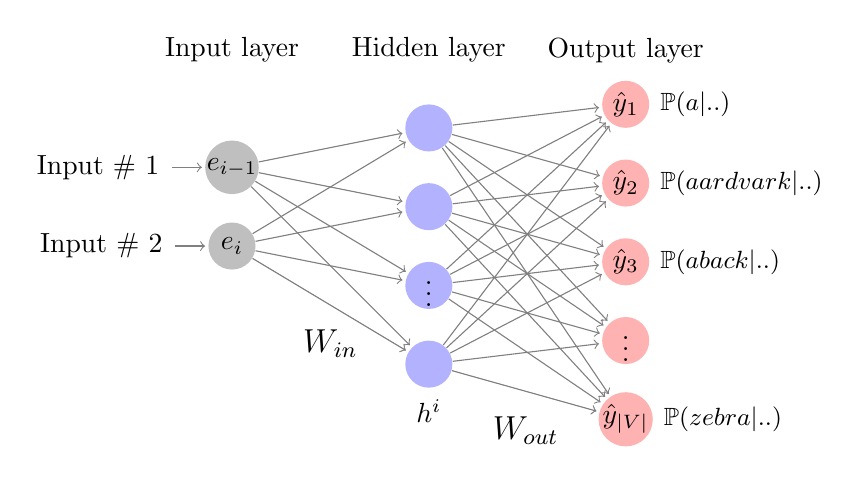
\begin{tikzpicture}[shorten >=1pt,->,draw=black!50, node distance=2.5cm]
\tikzstyle{every pin edge}=[<-,shorten <=1pt]
\tikzstyle{neuron}=[circle,fill=black!25,minimum size=17pt,inner sep=0pt]
\tikzstyle{input neuron}=[neuron, fill=gray!50];
\tikzstyle{output neuron}=[neuron, fill=red!30];
\tikzstyle{hidden neuron}=[neuron, fill=blue!30];
\tikzstyle{annot} = [text width=4em, text centered]
% Draw the input layer nodes
\node[input neuron, pin=left:Input \# 1] (I-1) at (0,-1) {$e_{i-1}$};
% Label above the first neuron
\node[above of=I-1, node distance=1.5cm] {Input layer};

% Draw the second input neuron with label $e_i$
\node[input neuron, pin=left:Input \# 2] (I-2) at (0,-2) {$e_i$};
% Draw the hidden layer nodes
\foreach \name / \y / \content in {1/1/, 2/2/,  3/3/\vdots, 4/4/}
\path[yshift=0.5cm]
node[hidden neuron] (H-\name) at (2.5cm,-\y cm) {$\content$};
% Label above the first neuron
\node[above of=H-1, node distance=1cm] {Hidden layer};

% Draw the output layer node
\foreach \name / \y / \content in {1/1/\hat{y}_1, 2/2/\hat{y}_2, 3/3/\hat{y}_3, 4/4/\vdots, 5/5/\hat{y}_{|V|}}
\path[yshift=0.8cm]
node[output neuron] (O-\name) at (5cm,-\y cm) {$\content$};
\node[above of=O-1, node distance=0.68cm] {Output layer};
\node[below of=H-4, node distance=0.6cm] {$h^i$};

\node[right=0.01cm of O-1] {\small $\mathbb{P}(a|..)$};
\node[right=0.01cm of O-2] {\small $\mathbb{P}(aardvark|..)$};
\node[right=0.01cm of O-3] {\small $\mathbb{P}(aback|..)$};
\node[right=0.01cm of O-5] {\small $\mathbb{P}(zebra|..)$};


% Connect every node in the input layer with every node in the hidden layer.
\foreach \source in {1,...,2}
\foreach \dest in {1,...,4}
\path (I-\source) edge (H-\dest);
% Connect every node in the hidden layer with the output layer
\foreach \source in {1,...,4}
\foreach \dest in {1,...,5}
\path (H-\source) edge (O-\dest);

\draw[->,gray,line width=0.1pt] (I-2) -- node[midway,below,yshift=-0.2cm,text=black] {\large $W_{in}$} (H-4);
\draw[->,gray,line width=0.1pt] (H-4) -- node[midway,below,yshift=-0.2cm,text=black] {\large $W_{out}$} (O-5);
\end{tikzpicture}
    \caption{Forward inference in a feed-forward neural language model with window size of two, at timestep $i+1$. To predict the next word $w_{i+1}$, the model concatenates embeddings of the two preceding words, $\ivec{e}_{i}$ and $\ivec{e}_{i-1}$, multiplies them by $\ivec{W}_{in}$, and applies an activation function to produce the hidden layer. This layer is then transformed by $\ivec{W}_{out}$ and a softmax to estimate the probability of each word in its vocabulary being the next word $w_{i+1}$.}
    \label{fig:nn_graph}
\end{figure}

\vspace{-0.5\baselineskip}
\paragraph{\ac{FFNLM}} The FFNLM applies a feed-forward neural network, a subtype of NN with unidirectional information flow (i.e., without looping back or cycles), for language modeling~\citep{ffnlm_bengio}. Similar to n-gram models, it employs a Markov assumption by considering a fixed number of previous words as context to predict the next word. In this model, words are first transformed into word embeddings. The embeddings from preceding $k$ words are then fed into a feed-forward neural network, which in turn produces a probability distribution over possible next words. For instance, Figure~\ref{fig:nn_graph} illustrates how to predict the next word $w_{i+i}$ in an FFNLM with a context window size of $k=2$. Formally, the defining equations at timestep $i+1$ are:
\begin{align}
      P(w_{i+1}|w_{i-1}w_{i}) &= \textsc{softmax}(\ivec{W}_{out}\ivec{h}^{i}+\ivec{b}_{out}) \nonumber \\
      \ivec{h}^{i} &= g( \ivec{W}_{in}
                 \begin{bmatrix}
                   \ivec{e}_{i}\\
                   \ivec{e}_{i-1}
                   \end{bmatrix}+\ivec{b}_{in})
\end{align}
\noindent where $W_{in} \in \mathbb{R}^{d_h \times 2d}$, $W_{out} \in \mathbb{R}^{|V| \times d_h}$, with $d_h$ denoting the hidden layer size, $d$ the embedding size, $|V|$ the vocabulary size and $g$ refers to the activation function.

However, despite being an advance over n-gram models, FFNLMs still have a fixed context size, which restricts their ability to capture long-range dependencies in text.

\paragraph{RNN language model} \ac{RNN} language models~\citep{elman1990finding,mikolov2010recurrent} overcome the limitations of the Markov assumption through recurrence. Unlike the feed-forward model, an RNN iteratively updates its hidden layers to capture information about the previous steps in the sequence. It processes the text one element at a time, predicting the next word based on the current word and the previous hidden state. Theoretically, this allows the model to retain information from the sentence's start to the present word, eliminating fixed context size constraints. As shown in Figure~\ref{fig:rnn}, while the forward inference of RNN is very similar to that of feed-forward NLM, the key distinction lies in the RNN's capacity to maintain and use a memory of prior timesteps through its hidden states. Formally, the defining equations at timestep $i+1$ are:
\begin{align}
      \mathbb{P}(w_{i+1}|{\color{red} w_{1}}\ldots w_{i}) &=
        \textsc{softmax}(\ivec{W}_{out}\ivec{h}^{i}+\ivec{b}_{out}) \nonumber\\
      \ivec{h}^{i} &= g( \ivec{W}_{in} \ivec{e}_{i} +\ivec{b}_{in} +\ivec{W}_{rec} \ivec{h}^{i-1}   )
\end{align}
\noindent Here, $\ivec{h}^{i}$ is an update of $\ivec{h}^{i-1}$, integrating the information from the current word, $\ivec{e}_{i}$. Essentially, $\ivec{h}^{i}$ can be considered as a vector encoding the information from the starting word $e_1$ up to the current word $e_i$.

\begin{figure}[ht]
\centering
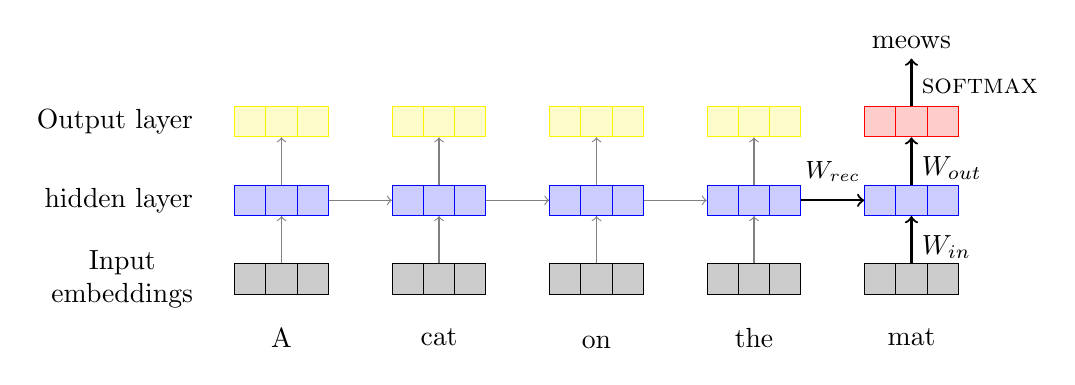
\begin{tikzpicture}[
      neurons/.style 2 args={
        rectangle split,
        rectangle split horizontal,
        draw=#2,
        rectangle split parts=#1,
        fill=#2!20}]

\node[neurons={3}{yellow}] (s1) at (0,2) {};
\node[neurons={3}{yellow}] (s2) at (2,2) {};
 \node[neurons={3}{yellow}] (s3) at (4,2) {};
 \node[neurons={3}{yellow}] (s4) at (6,2) {};
 \node[neurons={3}{red}] (s5) at (8,2) {};
\node (w6) [above=8mm of s5.center] {meows};
      
 \node[neurons={3}{blue}] (h1) at (0,1) {};
 \node[neurons={3}{blue}] (h2) at (2,1) {};
 \node[neurons={3}{blue}] (h3) at (4,1) {};
 \node[neurons={3}{blue}] (h4) at (6,1) {};
 \node[neurons={3}{blue}] (h5) at (8,1) {};

 \node[neurons={3}{black}] (x1) at (0,0) {};
 \node[neurons={3}{black}] (x2) at (2,0) {};
 \node[neurons={3}{black}] (x3) at (4,0) {};
 \node[neurons={3}{black}] (x4) at (6,0) {};
 \node[neurons={3}{black}] (x5) at (8,0) {};

  \node (w7) [left=10mm of x1.center,align=center] {Input \\ embeddings};
  \node (w8) [left=10mm of h1.center,align=center] {hidden layer};
  \node (w9) [left=10mm of s1.center,align=center] {Output layer};

  \node (w1) [below=5mm of x1.center] {A};
 \node (w2) [below=5mm of x2.center] {cat};
 \node (w3) [below=6mm of x3.center] {on};
 \node (w4) [below=5mm of x4.center] {the};
 \node (w5) [below=5mm of x5.center] {mat};
\draw [->,thick] (s5) -- (w6)node[pos=0,right,yshift=7pt] {\textsc{softmax}};

\draw [->,gray] (x1) -- (h1);
\draw [->,gray] (x2) -- (h2);
\draw [->,gray] (x3) -- (h3);
\draw [->,gray] (x4) -- (h4);
\draw [->,thick] (x5) -- (h5)node[pos=0,right,yshift=6pt] { $\ivec{W}_{in}$};


\draw [->,gray] (h1) -- (s1);
\draw [->,gray] (h2) -- (s2);
\draw [->,gray] (h3) -- (s3);
\draw [->,gray] (h4) -- (s4);
\draw [->,thick] (h5) -- (s5)node[pos=0,right,yshift=6pt] { $\ivec{W}_{out}$};

\draw [->,gray] (h1) -- (h2);
\draw [->,gray] (h2) -- (h3);
\draw [->,gray] (h3) -- (h4);
\draw [->,thick] (h4) -- (h5)node[pos=0.5,above,yshift=3pt] {\small $\ivec{W}_{rec}$};
\end{tikzpicture}
\caption{Forward inference in an RNN language model at timestep $i+1$. To predict the next word after the context ``A cat on the mat'', the model takes the embedding of the current word `mat' and multiplies it by $W_{in}$. Concurrently, it multiplies the hidden layer of the previous timestep $h_{i-1}$ by $W_{rec}$. These values are summed and passed through an activation function to produce the current hidden layer, $h^i$, which is then transformed by $\ivec{W}_{out}$ and a softmax to produce a probability distribution over the vocabulary.}\label{fig:rnn}
\end{figure}

RNNs, with their recurrent nature, can capture longer dependencies but face challenges with extended sequences due to the vanishing or exploding gradient issue. The \ac{LSTM} network, an advanced RNN variant, tackles the gradient problems through its sophisticated gated architecture. This structure helps the model decide when to keep or discard information across longer sequences, enhancing its ability to handle long-distance dependencies. Even with these improvements, LSTM still struggles with very long sequences. 
 

\paragraph{Transformer-based language models} Introduced by~\citep{NIPS2017_3f5ee243}, the Transformer architecture has revolutionized NLP. At the heart of the Transformer architecture is the self-attention mechanism, detailed in Subsection~\ref{sec:auto_transformer}, which theoretically allows each word to relate directly with every other word, irrespective of distance. The original model consists of an encoder-decoder structure, where the encoder is trained to convert input sequences into contextualized representations, while the decoder generates task-specific output sequences, using the previous output for context at each step. This design, often referred to as \ac{Seq2Seq}, is intended for Seq2Seq tasks, such as machine translation and text summarization. 

Due to its parallel processing capability and the ability to capture long-range dependencies effectively, the Transformer architecture has been adapted for language modeling~\citep{radford2018gpt1,radford2019language,devlin-etal-2019-bert} and has become the foundation for modern NLMs. Language modeling in Transformer models can be broadly categorized into two types: autoregressive and masked.

Autoregressive Transformer language models, such as the \ac{GPT} series~\citep{radford2018gpt1,radford2019language,brown2020language,openai2023gpt4} and more recent LLaMa~\citep{touvron2023llama}, predict the next word in a sequence based on all preceding words. They typically use only the decoder component of the original Transformer and are widely applied in natural language generation tasks. The main project of this dissertation (\S\ref{chp:main_project}) focuses on a GPT2-like autoregressive Transformer LM, and we test LLaMa in our SLOG project (\S\ref{chp:slog}). 

In contrast, masked Transformer language models such as \ac{BERT}~\citep{devlin-etal-2019-bert}, FlauBERT~\citep{le2019flaubert}, generate token representations by considering both prior and subsequent tokens in a sequence. They are pre-trained using a \textbf{masked language modeling objective},\footnote{Also called ``denoising'' objectives~\citep{taylor1953cloze}} where a certain percentage of input tokens are masked and the model is trained to predict these masked tokens from their surrounding context. These models are typically built using the encoder layers of the original Transformer. While they don't directly model the probability of input sequences as autoregressive models do, making them less suited for generation tasks, they excel at generating contextually rich token representations, widely used in natural language understanding tasks. 

Blending the strengths of both approaches, Seq2Seq language models like T5~\citep{2020t5} frame all NLP tasks as text-to-text problems. During pre-training, various spans of text are masked (similar to BERT), and then the model is trained to predict full sequences autoregressively. This dual nature makes them versatile and suitable for a wide range of NLP tasks, from text generation to classification and translation. We test the structural generalization ability of T5 in Chapter~\ref{chp:slog}.

Transformer-based pre-trained language models have become foundational elements in modern NLP systems due to their ability to learn generic transferable linguistic representations from vast unlabeled text corpora~\citep{kalyan2021ammus}. % and then transfer this knowledge to downstream tasks. 
Such contextualized representations can be used directly as inputs for task-specific text processing models. The transfer-learning paradigm, which includes pre-training followed by various fine-tuning methodologies~\citep{devlin-etal-2019-bert,pruksachatkun2020intermediate,liu2019multi}, further equips these models with task-specific knowledge. More recently, prompt tuning has emerged as an efficient technique that exploits these models to generate context-aware outputs from given prompts~\citep{liu2021pretrain}. Over the past couple of years, Transformer-based language models offer groundbreaking improvements in NLP capabilities, models like GPT-4 can generate coherent human-like text~\citep{bubeck2023sparks}. Moreover, they have inspired architectures in other domains, becoming a cornerstone in the expanding generative AI, which also includes image generation~\citep{ramesh2022hierarchical}, and code generation~\citep{chen2021evaluating}.

On the theoretical front, these contextualized representations have also become a focus of research on language and human language processing~\citeti{baroni2020linguistic,linzen2021syntactic,baroni2022proper,mccoy2018revisiting,liu-etal-2019-linguistic, yedetore-etal-2023-poor}. Researchers have leveraged these representations to investigate how these models process and understand language, what kind of linguistic knowledge they implicitly learn, and how their understanding aligns with or diverges from our knowledge of human language processing. The insights gained from such investigations can help inform both the design of more effective computational models and the theoretical understanding of human language.


\paragraph{Evaluation of language models} Perplexity is a probability-based metric to evaluate the quality of language model on its training task --- predicting next word based on previous words in a sequence. While a language model's performance can always be assessed through improvements in downstream applications, such extrinsic evaluation can be computationally expensive and affected by various task-specific factors. Intrinsic evaluation like perplexity provides a direct and more efficient way to measure the potential improvement of LMs, aiding in model development and comparison.

Formally, for a language model trained on a corpus and tested on a held-out test set, $\mathcal{D}_{t} = w_1, w_2, ..., w_N$, the model's perplexity $PPL$ on this test set is defined as the inverse probability of the test set, normalized by the number of words $N$:
\begin{align}
\mathbb{P}(\mathcal{D}_{t}) &= P(w_1, w_2, ..., w_N)^{-\frac{1}{N}} \nonumber \\
&= \left(\prod_{i=1}^{N} \frac{1}{P(w_i | w_1, \ldots, w_{i-1})}\right)^{\frac{1}{N}}
\end{align}
In practice, working with log probabilities is often preferred as sequence probabilities can become extremely small through multiplication. As language models are typically trained to maximize the log likelihood of the corpus, this definition of perplexity corresponds to exponentiating the average negative log-likelihood:
\begin{equation}
P(W) = 2^{-\frac{1}{N} \sum_{i=1}^{N} \log_2 P(w_i | w_1, \ldots, w_{i-1})}
\end{equation}
Conceptually, perplexity can be viewed as the \textbf{weighted average branching factor} of a language. It represents the average number of plausible
subsequent words that can follow any given word sequence. Thus, the perplexity of a language model on a test set is the average number of equally probable word predictions that the model makes for each actual word in the test set. A lower perplexity score indicates a better language model.  

\subsection{Transformer-based neural language model}\label{sec:auto_transformer}
In the previous section, we have seen that various neural networks can be used for language modeling; in this section, we delve into the Transformer, the current state of the art architecture for language modeling, with a specific focus on the autoregressive variant.

\paragraph{Overview of the Transformer architecture}
Transformer-based models consist of a series of identical Transformer blocks stacked together. As shown in Figure~\ref{fig:transformer_layer}, a standard Transformer block has two main components: a self-attention layer, followed by a fully-connected feed-forward network. Each of these two sub-layers includes a residual connection and is followed by a layer normalization operation.

\begin{figure}[ht]
    \centering
    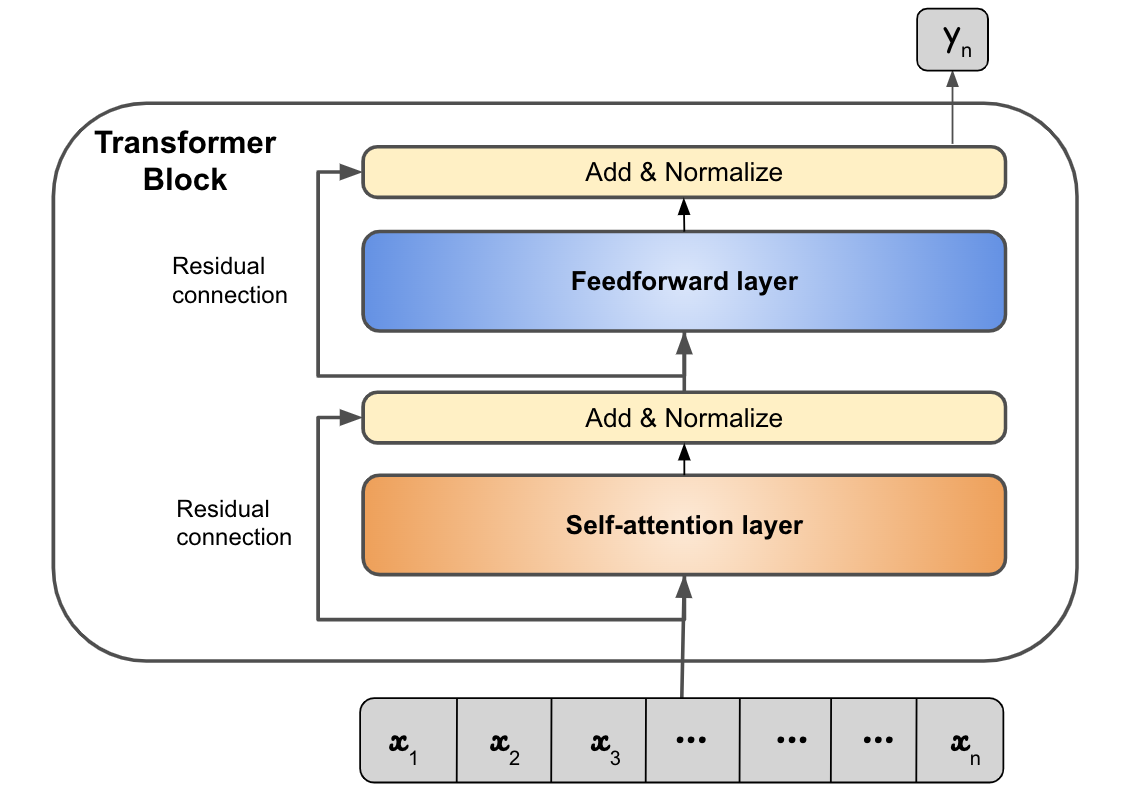
\includegraphics[scale=0.36]{figures/Transformer_layer.png}
    \caption{Components of a typical Transformer block: self-attention, feed-forward network, layer normalization, and residual connections. }
    \label{fig:transformer_layer}
\end{figure}
The self-attention layer, a key innovation of the Transformer architecture, enables the model to focus on different parts of the input when predicting the output for a particular position. This is accomplished by computing a weighted sum of the input sequence, where the weights are determined by the relevance 
of input elements related to the current position.

The feed-forward network (\S\ref{sec:lm_tasks}) applies a position-wise transformation to the attention outputs and allows the model to learn complex patterns. This transformation is the same at each position and includes two linear transformations with a relu activation function in between.

Residual connections play a crucial role in information preservation. These connections allow information from earlier layers to be passed unaltered to later layers, addressing issues such as vanishing gradients~\citep{he2016deep}. Specifically, in Transformer blocks, the output of each sub-layer (self-attention and feed-forward network) is added to its input before being normalized. Layer normalization~\citep{ba2016layer} is applied to these summed vectors to maintain the hidden layer values within an optimal range for gradient-based training. This process involves transforming the inputs to achieve a mean of 0 and a standard deviation of 1 across each layer.


The original Transformer consists of both encoder and decoder stacks, with each stack containing six identical Transformer layers. Early adaptations of Transformer-based models typically stack $l \in \{6, 10,12,16,24\}$ such layers, while the rise of large language models such as GPT-3 has led to architectures with nearly a hundred layers or more~\citep{brown2020language,openai2023gpt4}. In addition to these Transformer blocks, the model includes an input and output embedding layer. The input embedding layer converts each word in the input sequence to a high-dimensional vector, which is then combined with its position encoding to incorporate word order within the sequence. The output layer, on the other hand, is a linear layer followed by a softmax function to produce a probability distribution over the vocabulary for the next word prediction.

A standard formulation of the full Transformer stack is as follows:
\begin{align}
\text{For each layer } l = 1 \text{ to } L:& \nonumber \\
\text{Self-Attention: } & \mathbf{Z}_l^{(1)} = \text{SelfAttn}(\mathbf{Z}_{l-1}) + \mathbf{Z}_{l-1} \nonumber \\
\text{Normalization: } & \mathbf{Z}_l^{(2)} = \text{LayerNorm}(\mathbf{Z}_l^{(1)}) \nonumber \\
\text{Feed Forward: } & \mathbf{Z}_l^{(3)} = \text{FFN}(\mathbf{Z}_l^{(2)}) + \mathbf{Z}_l^{(2)} \nonumber \\
\text{Normalization: } & \mathbf{Z}_l = \text{LayerNorm}(\mathbf{Z}_l^{(3)})
\end{align}
\noindent where $l$ is the layer number, $L$ is the total number of layers, $\mathbf{Z}_l^{(1)}$ is the output of the self-attention mechanism at layer $l$, $\mathbf{Z}_l^{(2)}$ is the normalized self-attention output, $\mathbf{Z}_l^{(3)}$ is the output of the feed-forward network at layer $l$, and $\mathbf{Z}_l$ is the final output of layer $l$ after normalization.

\paragraph{Self-attention mechanism} The core principle behind the attention-based approach is its ability to assess the relevance of different elements within a sequence in relation to a target element. Let's consider an example sentence, ``The cat on the mat ate a fish". As shown in Figure~\ref{fig:self_attention_illu}, while predicting the next word after ``ate", self-attention draws comparisons between the current word ``ate" and all preceding words, including itself. Each pair of words is then assigned a relevance score, which can be calculated as a dot product. 
To compute the final representation for ``ate", the mechanism takes each word's vector representation seen so far, weighs it by the corresponding relevance score, and sums these weighted representations. As a result, words that are more relevant to ``ate" will contribute more to its final representation. 

\begin{figure}[ht]
    \centering 
\scalebox{0.8}{
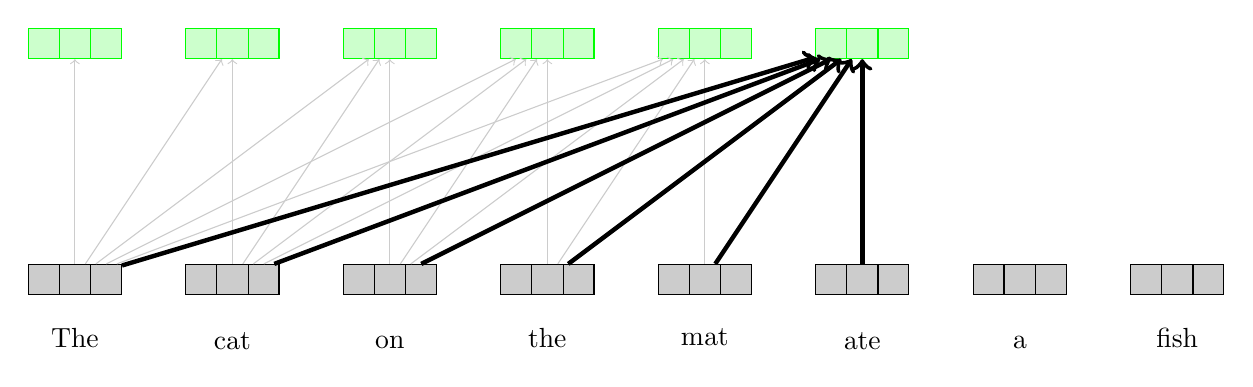
\begin{tikzpicture}[
      neurons/.style 2 args={
        rectangle split,
        rectangle split horizontal,
        draw=#2,
        rectangle split parts=#1,
        fill=#2!20}]
      
 \node[neurons={3}{green}] (s1) at (0,3) {};
 \node[neurons={3}{green}] (s2) at (2,3) {};
 \node[neurons={3}{green}] (s3) at (4,3) {};
 \node[neurons={3}{green}] (s4) at (6,3) {};
 \node[neurons={3}{green}] (s5) at (8,3) {};
 \node[neurons={3}{green}] (s6) at (10,3) {};
 %\node[neurons={3}{green}] (s7) at (12,3) {};

%\node (o1) [above=5mm of s7.center] {$target$};

 \node[neurons={3}{black}] (x1) at (0,0) {};
 \node[neurons={3}{black}] (x2) at (2,0) {};
 \node[neurons={3}{black}] (x3) at (4,0) {};
 \node[neurons={3}{black}] (x4) at (6,0) {};
 \node[neurons={3}{black}] (x5) at (8,0) {};
 \node[neurons={3}{black}] (x6) at (10,0) {};
 \node[neurons={3}{black}] (x7) at (12,0) {};
 \node[neurons={3}{black}] (x8) at (14,0) {};

  \node (w1) [below=5mm of x1.center] {The};
 \node (w2) [below=5.5mm of x2.center] {cat};
 \node (w3) [below=6mm of x3.center] {on};
 \node (w4) [below=5mm of x4.center] {the};
 \node (w5) [below=5mm of x5.center] {mat};
  \node (w6) [below=5.5mm of x6.center] {ate};
 \node (w7) [below=6mm of x7.center] {a};
 \node (w8) [below=5mm of x8.center] {fish};

\draw [->, color=gray!40] (x1) -- (s1);


\draw [->,color=gray!40] (x1) -- (s2);
\draw [->,color=gray!40] (x2) -- (s2);


\draw [->,color=gray!40] (x1) -- (s3);
\draw [->,color=gray!40] (x2) -- (s3);
\draw [->,color=gray!40] (x3) -- (s3);

\draw [->,color=gray!40] (x1) -- (s4);
\draw [->,color=gray!40] (x2) -- (s4);
\draw [->,color=gray!40] (x3) -- (s4);
\draw [->,color=gray!40] (x4) -- (s4);

\draw [->,color=gray!40] (x1) -- (s5);
\draw [->,color=gray!40] (x2) -- (s5);
\draw [->,color=gray!40] (x3) -- (s5);
\draw [->,color=gray!40] (x4) -- (s5);
\draw [->,color=gray!40] (x5) -- (s5);

%\draw [->,color=gray!40] (x1) -- (s6);
%\draw [->,color=gray!40] (x2) -- (s6);
%\draw [->,color=gray!40] (x3) -- (s6);
%\draw [->,color=gray!40] (x4) -- (s6);
%\draw [->,color=gray!40] (x5) -- (s6);
%\draw [->,color=gray!40] (x6) -- (s6);

\draw [->,ultra thick] (x1) -- (s6);
\draw [->,ultra thick] (x2) -- (s6);
\draw [->,ultra thick] (x3) -- (s6);
\draw [->,ultra thick] (x4) -- (s6);
\draw [->,ultra thick] (x5) -- (s6);
\draw [->,ultra thick] (x6) -- (s6);
%\draw [->,ultra thick] (x7) -- (s7);
\end{tikzpicture}
}
\caption{Masked self-attention in autoregressive Transformer language models: each token is processed considering all the preceding tokens and itself, future tokens are excluded.}
    \label{fig:self_attention_illu}
\end{figure}

Transformers introduce a more sophisticated way of representing how each word contributes to the understanding of other words within a sequence. The attention process discerns three distinct roles: the \textbf{query} (Q), the \textbf{key} (K), and the \textbf{value} (V). The query corresponds to the current focus of attention, the key represents the preceding input item being compared to the attention focus, and the value is employed to compute the output for the current position. To capture these three roles, the self-attention mechanism uses three weight matrices $\ivec{W}^q$, $\ivec{W}^k$, $\ivec{W}^v$, which are learned during the training. They transform each input vector to represent its specific role as a query, key, or value. Given these projections, the score between a current word $x_i$, and a token in the preceding context, $x_j$, is computed as the dot product of their respective \textbf{query} and \textbf{key} vectors --- $q_i \cdot k_j$. To achieve more stable gradients, this score is normalized by dividing it by the square root of the key vectors' dimension. Given a query and the set of keys, \{ $k_1,k_2,...,k_i$ \}, these individual scores are then passed through a softmax function to obtain the attention distribution:   

\begin{equation}
\alpha_1\ldots \alpha_i = \textsc{softmax} \left ( \frac{q_i \cdot k_1}{\sqrt{d_k}},\ldots,\frac{q_i \cdot k_i}{\sqrt{d_k}} \right ) 
\end{equation}
 
\noindent This attention distribution is then used to weigh the respective \textbf{value} vectors of the tokens. The result is a weighted sum of all the \textbf{value} vectors, which serves as the output of the self-attention mechanism for the token under consideration. This process is formally expressed as:

\begin{equation}
y_i = \sum_{j \leq i}{\alpha_{j} \cdot V_j}
\end{equation}

\noindent Since each output $y_i$ is computed independently, this entire attention process can be parallelized using matrix multiplication by considering all the $N$ tokens of the input sequence as a single matrix $X \in \mathbb{R}^{N \times d}$. The entire self-attention process for a sequence of $N$ tokens is computed as:

\begin{equation}
\text{SelfAttention}\left(\ivec{Q},\ivec{K},\ivec{V}\right) = \textsc{softmax} \left (\frac{\ivec{Q} \cdot \ivec{K}^T}{\sqrt{d_k}} \right ) \ivec{V}
\end{equation}

Masked Transformer LMs directly use this self-attention computation. However, the autoregressive Transformer has to maintain the autoregressive property, where a token's prediction relies only on preceding tokens and not future ones. To achieve this, a causal attention mask is applied. The causal mask matrix is formally defined as:
\begin{equation}
\textsc{mask}_{ij} = \begin{cases}
-\infty & \text{if } j > i \\
 0 & \text{otherwise}
\end{cases}
\end{equation}
\noindent Here, the upper triangle (future positions related to the current token), is filled with negative infinity and the lower triangle has zeros. Incorporating this causal mask, the output of a single self-attention layer becomes:
\begin{equation}
\text{SelfAttention}\left(\ivec{Q},\ivec{K},\ivec{V}\right) = \textsc{softmax} \left (\frac{\ivec{Q} \cdot \ivec{K}^T}{\sqrt{d_k}} + \textsc{mask} \right ) \ivec{V}
\end{equation}
\noindent Here, adding a very large negative number (from the mask) to the future positions, ensures that when the softmax function is applied in the next step, these positions will have an attention score of nearly 0. This forces the self-attention mechanism to attend only to its previous words and itself, thereby preventing information flow from any future words. This causal attention mask, as suggested by ~\cite{haviv-etal-2022-transformer} may implicitly introduce positional information into the self-attention layer.


Words within a sentence are interconnected in multiple ways. Consider the sentence ``The cat on the mat ate a fish", the verb ``ate" has a subject-verb syntactic dependency with ``cat" and also shares a semantic relationship, where ``cat" is the agent of the action. %, not the ``mat". 
To capture these different aspects of the syntactic, semantic, and even discourse relationships simultaneously, the Transformer employs multi-head attention. Specifically, each of the $h$ attention heads in a self-attention layer uses its unique learned set of weight matrices: $\ivec{W}_h^K$,$\ivec{W}_h^Q$ and $\ivec{W}_h^V$, to determine the respective \textbf{query}, \textbf{key}, and \textbf{value} vectors. Consequently, the output of the multi-head layer with $h$ heads consists of $h$ distinct vectors, each representing a different facet of the token's contextual relationships. For instance, one head might focus on learning grammatical structures, while another might specialize in capturing thematic relationships. These head-specific outputs are then concatenated and linearly transformed via $\ivec{W}^O$, to produce the final output for each token.

In mathematical terms, for an attention head $i$, the output, $\textsc{head}_i$, for a given sequence of N tokens, $X \in \mathbb{R}^{N \times d}$, is computed as follows:
\begin{align}
\textsc{head}_i = \text{SelfAttention}\left(\ivec{Q},\ivec{K},\ivec{V}\right) \nonumber \\
\ivec{Q} = \ivec{X}\ivec{W_i^Q}; \ivec{K} = \ivec{X}\ivec{W_i^K};\ivec{V} = \ivec{X}\ivec{W_i^V} 
\end{align}
where $\ivec{W_i^Q} \in \mathbb{R}^{d \times d_k}, \ivec{W_i^K} \in \mathbb{R}^{d \times d_k},\ivec{W_i^V} \in \mathbb{R}^{d \times d_v}$ with $d$ denoting the dimensionality of both the input to and output from the model, $d_k$ for the key and query embedding dimensions and $d_v$ for the value embedding dimension. Outputs from each head are concatenated and linearly transformed, producing the final output of a multi-head attention layer: 
\begin{equation}
    \text{MultiHeadAttention}\left(X\right) = \left(\textsc{head}_1 \oplus \textsc{head}_2,...,\oplus \textsc{head}_h \right) \ivec{W}^O
\end{equation}

\noindent where $\ivec{W}^O \in \mathbb{R}^{hd_v \times d}$, and $h$ is the total number of attention heads, $\oplus$ denotes the concatenation operation.


\paragraph{Position embeddings} Unlike RNN, which inherently handles word order information by processing input sequences one element at a time, the Transformer architecture is inherently agnostic to the order of tokens by considering all tokens in the input sequence simultaneously. However, the order of words is crucial to the semantics and syntax of a sequence and is often crucial in many tasks, such as language modeling and sequence-to-sequence translation. To overcome this limitation and inject some sense of position or order into the model, position embeddings were introduced.

One straightforward solution is to directly add positional embeddings to the input embeddings. Just as the model learns an embedding for a word like ``cat'', it can also learn a specific embedding for its position in a sequence such as ``The cat on the mat'', identifying it as the second word. In the original Transformer architecture, positional embeddings are generated using fixed sinusoidal functions. These functions convert integer positions into real-valued vectors, creating a unique positional embedding for each position. Specifically, each dimension of the positional embedding receives a value from a sine or cosine function of a different frequency. Formally, for position $p$ and dimension $i$, the values are defined as:
\begin{align}
    PE_{(p,2i)} &= \sin\left(\frac{p}{10000^{\frac{2i}{d}}}\right) \nonumber \\
    PE_{(p,2i+1)} &= \cos\left(\frac{p}{10000^{\frac{2i}{d}}}\right)
\end{align} %_{\text{model}} distance or difference
where $d$ is the dimension of the embeddings.  These fixed positional embeddings are then added to the standard word embeddings, giving the model a sense of each token's position in the sequence. This position encoding scheme has been extended to learned instead of fixed positional embedding in subsequent models such as BERT~\citep{devlin-etal-2019-bert}, Reformer~\citep{kitaev2020reformer}, RoBERTa~\citep{liu2019roberta}, etc. 

While absolute position embeddings provide a sense of sequence order, they don't directly capture the relative distances between tokens. For instance, by modifying ``the cat ate a fish'' to ``Yesterday, the cat ate a fish'', the absolute positions change but not the core meaning. What matters for meaning is the relative position between ``cat'' and ``fish'', regardless of their absolute position in the sequence. To better capture such relational dynamics, relative position embeddings are introduced~\citep{shaw-etal-2018-self,dai-etal-2019-transformer}. These embeddings shift the focus from the absolute position of a token in a sequence to the relative distances or positional differences between pairs of tokens.


Numerous subsequent models have proposed alternative position encoding schemes. For instance, some approaches integrate position information into the attention matrix instead of the input~\citep{dai-etal-2019-transformer,2020t5}. Others represent positions structurally based on the distances on a sentence's parse tree representation~\citep{wang-etal-2019-self,shiv2019novel}. Improving position representations is an ongoing research focus. The study by \cite{dufter-etal-2022-position} provides a comprehensive review of position encoding within the Transformer architecture.


\section{Analysis of linguistic structure in neural NLP models}\label{sec:review_structure_nlm}

The study of linguistic structures in computational models has a long history, dating back to the work of~\cite{elman1990finding,elman89representation} and~\cite{tabor1994syntactic}. Their pioneering research provided early evidence of the potential for neural networks to learn and embody abstract syntactic structures from non-annotated language data. Transitioning from these early insights to the modern era, the scale and complexity of current models like Transformers have significantly increased. As discussed in previous section, they generate output in the form of complex probability distributions over a large vocabulary of words or sub-words. This, in combination with their high-dimensional representation for inputs and millions of parameterized weights for operations, makes the interpretation of these models challenging.

In recent years, a myriad of analysis methods have been developed to better understand the inner mechanics of NLMs. Many studies suggest that these models have learned a substantial amount of syntactic knowledge that resembles human understanding, while others question the degree to which these models develop abstract structural representations of language. Although recent large language models demonstrate an apparently human-like ability to generate fluent and grammatically correct text~\citep{bubeck2023sparks}, there is yet no consensus on whether these Transformer-based models truly understand and incorporate the linguistic structure.

In this section, we will explore three core methods for interpreting and analyzing the representation of linguistic structure in neural NLP models and also discuss their associated limitations.

\subsection{Challenge sets} \label{sec:behav_test}
Challenge sets, also known as test suites, have a long-standing tradition in NLP, tracing back to work like~\cite{lehmann-etal-1996-tsnlp}. These carefully curated sets include a wide range of linguistic phenomena, often targeting specific syntactic, semantic, or pragmatic properties~\citeti{king-falkedal-1990-using,sennrich-2017-grammatical,isabelle-etal-2017-challenge,naik-etal-2018-stress}. While they were initially employed primarily for evaluating machine translation systems, the evolution and success of neural language models have broadened their application. Largely inspired by the experimental paradigms in psycholinguistics, challenge sets have become one of the important methodologies for investigating the fine-grained linguistic knowledge embodied within NLMs. This approach attempts to answer questions like: How well do neural language models capture linguistic principles, and to what extent do they exhibit human-like grammatical competence?


In psycholinguistics literature, a paradigmatic test for human syntactic capacity comes from agreement phenomena~\citep{bockRegulatingMentalEnergy1992, BOCK199145, bockAttractionsVerbAgreement2001}. For instance, subject-verb agreement in English as illustrated in (\ref{ex:na_en_s-v}): the form of the verb ``are'' is determined by its syntactic subject ``keys'', irrespective of the linear distance between them or the presence of the intervening noun, ``cabinet'', which carries a different grammatical number than the subject, and is often referred to as agreement \textit{attractor}~\citep{BOCK199145}. Such long-distance agreement phenomenon exemplifies the hierarchical organization of language rather than a simple linear structure~\citep{everaert2015}.

\setcounter{exx}{0} % Start numbering examples from 1
\begin{exe}
   \ex\label{ex:na_en_s-v}
The old rusty \textbf{keys} to the cabinet \textbf{are} on the table.
\end{exe}

\cite{linzen-etal-2016-assessing} pioneered the use of subject-verb agreement to assess the syntactic sensitivity of modern NLM. They collected 1.35 million English sentences with present-tense verbs from an auto-parsed Wikipedia corpus and annotated each with the main verb's grammatical number. The model's syntactic ability was then evaluated through a \ac{NA} prediction task. In this task, an LSTM took as input the sentence prefixes like the one in (\ref{ex:sent_prefix}), and was trained to predict the grammatical number of the subsequent verb, either \textit{Singular} or \textit{Plural}.

\vspace{-0.5\baselineskip}
\begin{exe}
   \ex\label{ex:sent_prefix}
The old rusty keys to the cabinet \underline{\ \ \ }
\end{exe}
\vspace{-0.5\baselineskip} 
Linzen and colleagues tested an LSTM with 50 hidden units and found that the model demonstrated near perfect overall accuracy on unseen sentence prefixes. Even in the most challenging cases with four attractors like  (\ref{ex:4_attr})\footnote{Agreement attractors are highlighted with an underline. The subject and target verb are marked in bold.}, the accuracy of the number prediction was still 82\%. 
\vspace{-0.5\baselineskip}
\begin{exe}
   \ex\label{ex:4_attr}
Yet the \textbf{ratio} of \underline{men} who survive to the \underline{women} and \underline{children} who survive in these \underline{events} \textbf{is} not clear. 
\end{exe}
\vspace{-0.5\baselineskip}
From these results, the authors concluded that LSTM models, when provided with explicit supervision, can capture significant grammatical structures, enabling them to reasonably approximate structure-sensitive dependencies.

Building on this experimental approach, \cite{gulordava-etal-2018-colorless} further showed that such long-distance agreement is learnable for an LSTM trained on language modeling (i.e., without explicit supervision). Subsequent research has delved deeper into understanding the capability of NLMs to abstractly represent sentence structures during agreement resolution. This exploration spans various dimensions: different languages~\citep{ravfogel-etal-2018-lstm,gulordava-etal-2018-colorless,lakretz2021mechanisms}, diverse models \citep{bernardy-lappin-2017-using,goldberg19assessing}, and potential confounding factors such as lexical co-occurrences~\citep{gulordava-etal-2018-colorless,lasri-etal-2022-bert} or surface-level heuristics \citep{kuncoro2018perils}. Our research contributes to this body of work, with a focus on French agreement phenomena and autoregressive Transformer LM~\citep{li-etal-2021-transformers}. The majority of these studies converge on the positive finding that neural language models are capable of learning a considerable amount of non-trivial structure information from the (unannotated) training data. More detailed discussions on related work that approaches long-distance agreement tasks can be found in Chapter~\ref{chp:NA_tasks}.

Another significant line of research has sought to expand this experimental approach beyond agreement phenomena to encompass a wider array of syntactic phenomena, such as anaphora, licensing, argument structure alternation, and filler-gap dependencies~\citeti{marvin-linzen-2018-targeted,kann-etal-2019-verb,warstadt-etal-2019-neural,wilcox-etal-2018-rnn,hu-etal-2020-systematic}. These studies typically create precisely drafted templates to generate challenge sets featuring specific linguistic phenomena, and then evaluate a neural network's grammaticality judgement on minimally differing sentence pairs based on grammaticality. Evaluations are conducted either through binary acceptability classification, similar to the number agreement prediction task proposed by~\cite{linzen-etal-2016-assessing}, or by comparing the probabilities that a language model assigns to whole sentences. More recently, \cite{warstadt-etal-2020-blimp} introduced BLiMP, a benchmark of linguistic minimal pairs covering a wide range of English grammatical phenomena. Generally, in these studies, NLMs' performance varies significantly across linguistic phenomena. While the models demonstrate robust knowledge of some syntactic phenomena, such as local subject-verb agreement, ellipsis, and control/raising, they struggle with more subtle semantic and complex syntactic phenomena, including licensing and extraction islands.


\paragraph{Formal languages} Analyzing NLMs' ability to handle linguistic structures is complex due to the intertwining of syntactic, semantic, and statistical regularities in human languages. To precisely focus on syntax-processing, researchers also employ formal languages in challenge sets. Typically, a study using formal languages designs a formal grammar to generate a corpus of sentences. A language model (\S\ref{sec:nlms}) is then trained on this corpus, and the evaluation focuses on the model's capability to recognize sequences from the training set and to generalize these learnings to unseen sequences.

Some studies focus on formal languages that correspond to specific classes in the Chomsky hierarchy, investigating which language classes can be theoretically or empirically learned by NLMs. Early studies have shown that certain regular~\citep{giles1992learning} and context-free~\citep{elman89representation} languages can be learned by different RNN models. Subsequent research found that, with proper parametrization, LSTM networks could learn context-sensitive languages, such as $a^nb^nc^n$, and generalize to longer sequences~\citep{gers2001lstm,weiss2018practical,suzgun-etal-2019-lstm}. In contrast, Transformer models have demonstrated, in theoretical studies, more limited capacities compared to LSTMs when handling regular languages and context-free languages~\citep{bhattamishra-etal-2020-ability,hahn:2020}. However, empirical findings like~\citep{ebrahimi-etal-2020-self} have shown that Transformers can
learn $Dyck_k$ languages from finite samples, matching the performance of LSTMs. 
% yao-etal-2021-self

Others craft formal grammars that mirror specific structures present in natural language. For instance, \cite{lakretz2021can} used a \ac{PCFG} to investigate RNN's ability to handle recursively nested subject-verb agreements, \cite{hupkes2020compositionality} used a set of PCFGs to assess NLMs' capacity in processing hierarchical compositional structure. Notably, \cite{sennhauser-berwick-2018-evaluating} evaluated LSTMs using bracket prediction tasks as a measure of understanding linguistic hierarchical structures.  While their findings confirmed that LSTMs can learn context-free grammar, they also observed that models' good performance stemmed more from efficiently handling nuisance variables rather than truly learning the underlying context-free rules. ~\cite{hahn:2020} has theoretically demonstrated that Transformer-based models struggle with bracket closing and iterated negation tasks, both computations are
considered to be essential to hierarchical structure.

\paragraph{Limitations} Challenge sets shed light on models' fine-grained linguistic capabilities by assessing their responses to specific inputs. However, this approach offers limited insight into the internal representations that the model has learned. Confounding factors, such as the inability to distinguish genuine syntactic comprehension from superficial pattern recognition like frequency-based heuristics, can make their results hard to interpret. To get a more comprehensive picture of NLMs' syntactic abilities, these tests should be supplemented with other methods, such as probing tasks or interpretability techniques that can provide insights into the models' internal workings.



\subsection{Probing classifiers} \label{sec:probing}
%probing tasks~\citep{conneau-etal-2018-cram}, 
 The probing classifier approach, also known as auxiliary prediction tasks~\citep{adi2016fine}, diagnostic classifiers~\citep{veldhoen2016diagnostic}, or linguistic probes~\citep{zhu-rudzicz-2020-information}, 
 is widely used to analyze the linguistic capabilities of neural NLP models. At its core, this approach involves training a classifier --- a ``probe'' --- on a model's internal representation to predict specific linguistic properties. Success in this prediction indicates that the model has encoded the relevant linguistic features. The basic premise is that if a model captures a particular linguistic property, this information should be extractable from its internal representation~\citep{hupkes2018visualisation}. This approach thus seeks to address the question: What linguistic properties are encoded in a model's internal representations, and where are they located within the model?

Formally, we define a model under investigation as a function, $\textsc{NN}:x \leadsto r$, that generates a representation, $r$, for an input element. A probing dataset, denoted as $\mathcal{D} = \{r^{(i)}, z^{(i)}\}$, pairs each representation with its associated linguistic property. The probing classifier can then be defined as a function $\mathcal{C}$ that maps the model's representation to a linguistic property of interest: 
\begin{equation}
    \mathcal{C}: r \leadsto z
\end{equation}

In an early application of this approach, \cite{shi-etal-2016-string} probed the syntactic information in neural machine translation. They extracted the hidden states of an RNN encoder and used them to train a logistic regression classifier, predicting labels related to morpho-syntax, such as PoS tags, constituent labels (e.g., NP, VP), voice, and tense. Their results, showing high probing accuracy relative to baseline measures, led them to conclude that the RNN captures significant syntactic information at both the word and sentence levels. Furthermore, they used probing classifiers to identify where syntactic information was stored across layers, observing that local features were often encoded in lower layers, while more abstract, global information was found in upper layers.

This probing methodology has since expanded to investigate other syntactic facets in RNN models, such as surface sentence structure~\citep{adi2016fine},\footnote{Surface sentence structure refers to sentence length, word identities and word order in ~\cite{adi2016fine}.} parse tree depth~\citep{conneau-etal-2018-cram}, syntactic agreement~\citep{giulianelli-etal-2018-hood} and even semantic properties~\citep{ettinger-etal-2016-probing}. This methodology has also been extensively applied to Transformer-based models~\citeti{tenney2019you,liu-etal-2019-linguistic,jawahar-etal-2019-bert,klafka-ettinger-2020-spying}. Collectively, these investigations have yielded promising results, consistently indicating that neural NLP models trained on vast data do encode a wide array of linguistic properties within their internal representations. An interesting extension of this methodology is the structural probe introduced by~\cite{hewitt-manning-2019-structural}. This probe, distinct yet related to the probing classifier, identified a linear transformation that could extract syntactic parse tree structures from word representation spaces in models like ELMo and BERT, but not from simpler baseline representations. (See Table~\ref{tab:probing_papers} for a categorization of representative work using the probing classifiers.)
%,manning2020emergent
\begin{table}[ht]
    \centering
    \scalebox{0.85}{  \begin{tabular}{p{0.22\textwidth}p{0.18\textwidth}p{0.18\textwidth}p{0.22\textwidth}p{0.18\textwidth}}
        \toprule
        \makecell[l]{Linguistic \\ properties} & \makecell[l]{Probing \\classifiers} & Probed models & Baseline models & Papers \\
        \midrule
        \makecell[l]{PoS, tense,voice, \\constituents} & \makecell[l]{Logistic\\ regression} & LSTM encoder & Phrase/syntax-based system & \cite{shi-etal-2016-string} \\
        \midrule
        \makecell[l]{Surface sentence \\ structure} & MLP &LSTM encoder & CBOW &\cite{adi2016fine}\\
        \midrule
        \makecell[l]{Surface structure,\\ parse tree depth,\\ top constituents} & MLP & \makecell[l]{BiLSTM, \\ConvNet }& Unigram, Human&\cite{conneau-etal-2018-cram} \\
         \midrule
        Syntactic agreement & Linear &LSTM LM& --&\cite{giulianelli-etal-2018-hood}\\
         \midrule
        \makecell[l]{PoS, \\dependency edge}&Linear \&MLP&ELMo&Control tasks&\cite{hewitt-liang-2019-designing}\\
        \midrule
        \makecell[l]{8 core NLP \\ labeling tasks} &MLP& \makecell[l]{CoVe, ELMo,\\GPT, BERT} &\makecell[l]{Lexical baselines,\\randomized ELMo,\\word-level CNN}&\cite{tenney2019you}\\
        \midrule
        Entire parse tree&Linear&ELMo, BERT& \makecell[l]{Non-contextual\\ models}&\cite{hewitt-manning-2019-structural}\\
        \bottomrule
    \end{tabular} }
    \caption{A categorization of some representative studies using probing classifiers to investigate syntactic structures in NLMs, according to linguistic properties examined, classifier types, probed models, and baseline models.}
    \label{tab:probing_papers}
\end{table}

On the other hand, recent studies also highlight potential pitfalls in the probing classifier approach, emphasizing that learned properties should be interpreted in comparison to control baselines. This can be achieved through techniques such as training probes on randomized representations~\citep{conneau-etal-2018-cram,tenney2019you}, using control functions~\citep{hall-maudslay-etal-2020-tale}, or implementing control tasks~\citep{hewitt-liang-2019-designing,ravichander-etal-2021-probing}. Specifically, control tasks are designed in a way that they can only be solved if the probe memorizes the task. Based on this, \cite{hewitt-liang-2019-designing} introduced the concept of \textit{selectivity}, which is defined as the performance gap between a probing task and its control counterpart. Using this metric to guide probe selection, they found that, while linear probes are highly selective, nonlinear probes are generally less so. The effectiveness of such probes with respect to its complexity remains a topic of discussion~\citep{hall-maudslay-etal-2020-tale,ravichander-etal-2021-probing},~\cite{belinkov-2022-probing} provides a comprehensive review on probing methods. 


\paragraph{Limitations} A main limitation of probing classifiers is that they only reveal correlations between linguistic properties and a network's inner representations, but do not necessarily indicate causality. Since these probes operate independently from the model's original task, they do not provide any insight on whether the information discovered by the probe influences the model's predictions. Only a few studies we have seen so far, like the one by~\cite{giulianelli-etal-2018-hood}, address this limitation; we will further explore and categorize such efforts in the following subsection, focusing on the causal analysis approach.


\subsection{Causal intervention analysis} \label{sec:sota_causal_approaches}

While linguistic probes are instrumental in revealing what linguistic properties might be encoded within neural models, they often fail to establish a causal relationship between these properties and the probed model's prediction. Causal intervention analysis fills this gap: it assesses the direct influence of specific model components on predictions by manipulating parts of the model and tracking resultant output changes. In this way, we can answer the causal question: which information is actually being used by neural models? Causal analysis is commonly paired with behavioral tests or probing tasks, providing a comprehensive framework for both uncovering and validating the model's linguistic behaviors.

Causal interventions in neural models vary based on where they are applied within the model. Broadly, these interventions can be grouped into three categories: 
\begin{itemize}
    \item Input-level interventions~\citep{zmigrod-etal-2019-counterfactual,vig2020causal,amini2023naturalistic}
    \item layer-level interventions~\citeti{giulianelli-etal-2018-hood,elazar2021amnesic,vig2020causal,ravfogel-etal-2021-counterfactual,feder-etal-2021-causalm}
    \item neuron unit-level interventions~\citep{bau2018identifying,lakretz-etal-2019-emergence,vig2020causal,mueller-etal-2022-causal}
\end{itemize}

In one of the pioneering works, \cite{giulianelli-etal-2018-hood} combined causal intervention with probing classifiers to explore an NLM's syntactic capabilities. They showed that by intervening on an NLM's internal representations --- guided by the gradients from a probing classifier targeting the subject's plurality --- the model's predictions in the subject-verb agreement task could be altered. Thus, the authors concluded that probing classifiers can identify features that are actually used by the model. Later, the study by \cite{elazar2021amnesic} presents a nuanced view. They explored the effects of erasing specific linguistic information from BERT's representation layers on language modeling. Using the iterative null space projection method (INLP; \cite{ravfogel-etal-2020-null}), they systematically erased linguistic information, such as Part-of-Speech and syntactic dependencies, from BERT's internal representations. The INLP process involves training (linear) probing classifiers to detect these linguistic properties and iteratively erasing the associated features until the representations are no longer predictive of the target property. When comparing the language modeling performance before and after such interventions, they observed that the removal of certain properties, such as phrase boundaries, which had high probing performance, didn't significantly impact language modeling performance. This led them to a conclusion contrasting with \cite{giulianelli-etal-2018-hood}: probing classifiers may not always detect information that the model actively uses for its predictions. 

Further expanding the scope, \cite{vig2020causal} explored gender bias in pre-trained Transformer LMs through a comprehensive causal intervention analysis. They manipulated the grammatical gender in the input, attention weights, and individual neurons to measure their causal impacts on the model's behavior. They found that gender bias predominantly resides in a small part of the network and this bias can be traced back to both direct input influences and indirect pathways via individual neurons and attention heads. The implications of this study extend beyond gender bias, offering a structural-behavioral framework for broader research aimed at interpreting and understanding the inner workings of neural NLP models.  

\paragraph{Limitations} Causal intervention analysis presents a unique perspective for establishing causality in interpreting deep NLP models, thus addressing certain limitations of challenge tests and probing classifiers. However, its implementation can be computationally expensive, especially in complex scenarios like neural-level interventions, and establishing clear cause-and-effect relationships within expansive networks is intricate. These complexities limit its practical application, particularly with state-of-the-art models.



\part{Assessing model capacity to represent syntactic structures }
\chapter{Long-distance agreement in neural language models}\label{chp:NA_tasks}

%\startcontents[chapters]


After surveying the landscape of various approaches and diverse conclusions on the linguistic capacities of neural NLP models, we now move into a focused review of one widely used approach: long-distance agreement tasks. This approach provides a compelling lens through which to investigate the ability of neural models to capture syntactic structure. At its core, syntactic agreement is a fundamental aspect of syntax,  where certain sentence elements must align in features like number, gender, or person. Long-distance dependencies inherently require an understanding of how components in a sentence relate across spans of text, and crucially, morphological cues
such as number and gender explicitly denote these long-term dependencies, offering a clear means to assess whether models effectively establish these connections.
 
In this chapter, we present several key studies that used the long-distance agreement paradigm --- especially subject-verb agreement --- to evaluate the ability of neural language models to capture syntactic information. 


Subject-verb agreement processing, a well-established paradigm in psycholinguistics, is commonly used to study human syntactic ability. Studies in this domain suggest that humans rely on hierarchical structures to ensure syntactic coherence~\citep{bockRegulatingMentalEnergy1992, BOCK199145, bockAttractionsVerbAgreement2001}. The work of \cite{elman89representation}, one of the first to analyze the syntactic capacity of neural networks, used the resolution of subject-verb agreement to demonstrate that a simple recurrent network is capable of encoding relevant grammatical relations and hierarchical structures in its distributed representation. This experimental approach, revitalized by the seminal work of \cite{linzen-etal-2016-assessing} (detailed in \S\ref{sec:behav_test}), has since been used in a tremendous number of works to explore the capacity of neural networks to capture abstract information about linguistic structures \citeti{wilcox-etal-2018-rnn,gulordava-etal-2018-colorless,giulianelli-etal-2018-hood,jumelet-etal-2019-analysing,lasri-etal-2022-probing}. 


\paragraph{Naturalistic data} Using this paradigm, early studies~\citep{linzen-etal-2016-assessing,bernardy-lappin-2017-using} showed that RNN models could handle the subject-verb number agreement task when given explicit supervision. Lately, \cite{gulordava-etal-2018-colorless}, expanding on \cite{linzen-etal-2016-assessing}, revealed that an LSTM language model, pre-trained only to predict the next word in an unannotated corpus, could effectively handle long-distance agreement in an unsupervised manner. 

Specifically, Gulordava and colleagues trained an LSTM language model on a corpus from Wikipedia with 100M tokens. This model was then tested on its ability to handle long-distance number agreements using sentences extracted from Universal Dependency treebanks. The evaluation method involves presenting the pre-trained model with sentence prefixes up to the target verb, and then comparing the probabilities that the model assigned to the singular and plural form of the target verb. For instance, in example (\ref{ex:compare_prob}), if the model predicts a higher probability for ``are'' over ``is'', it is deemed to have made the correct prediction for that sentence. Consequently, the overall accuracy for the agreement prediction task is calculated as the percentage of test instances in which the verb form with the higher probability is indeed the correct one.
%\vspace{-0.5\baselineskip}
\begin{exe}
   \ex\label{ex:compare_prob}
The old rusty keys to the cabinet \underline{\ \ \ }   \\
$\mathbb{P}(\textrm{\bf are}|\textrm{prefix}) >
      \mathbb{P}(\textrm{\bf is}|\textrm{prefix})$ $\Rightarrow$ predict ``are" 
\end{exe}
%\vspace{-0.5\baselineskip}

\noindent Using this method, \cite{gulordava-etal-2018-colorless} showed that LSTM achieved high accuracy in various constructions in the four languages tested: English, Italian, Hebrew, and Russian. In the case of Italian, the authors also conducted experiments with human subjects. The performance of the LSTM language model was at pair with human performance. 

Furthermore, Gulordava and colleagues introduced a control setting to ensure that the model did not use collocational information to determine the correct verb form. For instance, in the sentence “The cats on the mat meow loudly”, a language model may prefer the correct agreement by encoding information about what typically meows (cats) and what does not (mat), without relying on the target abstract structural rule. Such a confounding factor could overstate model success and raise questions about whether surface statistical patterns rather than the intended abstract syntactic information are driving performance. \cite{chomsky1957syntactic} claimed that grammaticality should be considered as a pure matter of syntax and structure, independent from semantic meaning or significance. Therefore, a sentence like ``Colorless green ideas sleep furiously'', despite being nonsensical, remains grammatically well-formed. If a model can capture the syntactic structure exemplified by agreement phenomena in naturalistic datasets, it should also be able to learn the syntactic constraints of nonsensical sentences. Inspired by this concept, Gulordava and colleagues also evaluated LSTMs on grammatically well-formed yet semantically implausible test instances, with the same number agreement prediction task.
Specifically, a nonsensical evaluation set was created by replacing each content word of the original corpus-extracted sentence with a random word sharing the same PoS and
morphological features:   
%\vspace{-0.5\baselineskip}
\begin{exe}
   \ex\label{ex:nonce_ex}
\textsc{Original}: The old rusty keys to the cabinet (are$/*$is) ...   \\
\textsc{Nonce}: The colorless green ideas to the door (are$/*$is)... (paraphrasing Chomsky)
\end{exe}
%\vspace{-0.5\baselineskip}
Their results showed that LSTM model's performance on nonsensical sentences was only slightly lower than on original ones; in Italian, this difference was just 6.6\%, a similar performance drop was observed in human subjects. This highlights model's ability to predict agreement in the absence of lexical or semantic cues and thus rules out the possibility that the LSTM decisions relied solely on surface information.

\paragraph{Formal languages} Another way to isolate genuine syntactic processing from semantic information is to use formal languages. \cite{lakretz2021can} investigated RNN's ability to handle recursively nested subject-verb agreements, using artificial data generated by a PCFG. To illustrate, consider the example:
\begin{exe}
    \ex a2 a1 \textbf{n3[sg]} a5 a3 \textbf{n1[pl]} a2 a2 \textbf{v5[pl]} a4 a1 \textbf{v4[sg]} a2 a5
\end{exe}
Here, tokens starting with `a',`n' and`v' represent adjective-, noun- and verb-like tokens, respectively. Tokens marked with number information, highlighted in bold, ensure that nouns and verbs at each nested depth (in this case, depth$=2$) exhibit number agreement. The surrounding adjective-like tokens control dependency length, spanning two units in length on either side. Lakretz and colleagues created such training datasets, varying in terms of nested tree depths and dependency lengths. They then assessed RNN language models, trained with a language modeling objective, on subject-verb agreement tasks in controlled, incrementally challenging scenarios. Findings from this study indicated that while RNN language models could generalize to longer dependencies, they struggled with deeper tree structures.

\paragraph{Synthetic data} Given the sparsity of complex syntactic sentences in treebanks~\citep{gulordava-etal-2018-colorless} and the limited scope of the formal language approach, which often explores specific syntactic facets in artificial settings, the use of synthetic data becomes an appealing alternative. \cite{marvin-linzen-2018-targeted} developed a template-based syntactic evaluation dataset, which features pairs of sentences, identical in all respects except for their grammaticality as shown in~(\ref{ex:sent_mini_pair}), targeting diverse structures-sensitive phenomena. In exploring the subject-verb agreement, their work delved into well-controlled challenging scenarios, where intervening elements such as prepositional phrases, relative clauses, or verb phrase coordination, separate the target subject and verb. For evaluation, instead of solely comparing the probability an LM assigns to a pair of words, they assessed the probabilities of entire sentences, determining if the model favored the grammatical over the ungrammatical sentence. 
%\vspace{-0.5\baselineskip}
\begin{exe}
   \ex\label{ex:sent_mini_pair} $\mathbb{P}(\textrm{sentence a.}) \overset{?}{>}
      \mathbb{P}(\textrm{sentence b.})$ \\
\vspace{-0.8\baselineskip}
\begin{enumerate}[label=\alph*.]
    \item The farmer that the parents love swims.
    \item \raisebox{0.8ex}{\textasteriskcentered}The farmer that the parents love swim.
\end{enumerate}
\end{exe}
%\vspace{-0.5\baselineskip}

\noindent This evaluation method extends to scenarios where multiple words may contribute to ungrammaticality, such as negative-polarity items. Their findings highlighted that while RNN language models excelled at local subject-verb agreements (i.e., no attractor), they exhibited sensitivity to specific lexical items and faced difficulties with rarer patterns, such as agreement across an object relative clause. Subsequent studies broadened the scope to include other phenomena considered by linguists to be sensitive to hierarchical structures, such as argument structure alternation, and filler-gap dependencies, as detailed in Section~\ref{sec:behav_test}.

  
\paragraph{Abstract representations} On the other hand, several studies have pointed out the limitations of relying solely on the agreement prediction approach to assess the representation of abstract syntactic structures by neural models. For instance, \cite{kuncoro2018perils} found that artificial neural networks may exploit spurious correlation in agreement tests without actually acquiring the desired syntactic competence: In the test set from \cite{linzen-etal-2016-assessing}, the agreement controller is the first noun in 80\% of sentences with multiple \textit{attractors}. This means that a simplistic heuristic, like agreeing with the first noun, can handle most of the complex agreement cases.

In addition, \cite{newman-etal-2021-refining} raised concerns regarding the hand-crafted minimal pair setting commonly used in agreement prediction tasks. While evaluating models based on their agreement outputs does not provide insights on their internal representations, this minimal pair setting further limits this approach to systematically capture a model's syntactic behavior. For instance, when given the prefix ``The keys to the cabinet", the commonly used metric compares only one verb pair's probabilities: is/are, as illustrated in (\ref{ex:mini_pair_be}). However, this evaluation does not account for the model's overall probability distribution across vocabulary. So, even if a model correctly predicts ``are" for the \textit{be} pair, it could err in other contexts, such as favoring ``exists'' over ``exist'', as shown in (\ref{ex:mini_pair_exist}), when not restricted to choose specific verb forms. To assess the broader syntactic understanding of a model, complementary methodologies going beyond behavioral tests are required.

\vspace{-0.5\baselineskip}
\begin{exe}
   \ex\label{ex:mini_pair}
The keys to the cabinet \underline{\ \ \ }   \\
\begin{xlist}
    \vspace{-2ex}
    \ex \label{ex:mini_pair_be} $\mathbb{P}(\textrm{\bf are}|\textrm{prefix}) >
      \mathbb{P}(\textrm{\bf is}|\textrm{prefix})$ $\Rightarrow$ predict ``are", plural form \\
      \vspace{-2ex}
    \ex \label{ex:mini_pair_exist} $\mathbb{P}(\textrm{\bf exists}|\textrm{prefix}) >
      \mathbb{P}(\textrm{\bf exist}|\textrm{prefix})$ $\Rightarrow$ predict ``exists", singular form 
      %\vspace{-1.5ex}
      \end{xlist}
\end{exe}
\vspace{-0.5\baselineskip}

Delving deeper, another research strand has focused on exploring models internal representations and inner workings. \cite{giulianelli-etal-2018-hood} conducted one of the first studies to investigate mechanisms tracking subject-verb agreement in LSTMs. After replicating the number agreement experiments of \cite{gulordava-etal-2018-colorless}, they used probing classifiers~(\S\ref{sec:probing}) to analyze where and how LSTMs represented the agreement information:
Classifiers were trained to predict the number information of the target subject (`singular' or `plural') from LSTM's internal representations for all tokens in a sentence. The results revealed that in sentences where the LSTM accurately predicted the verb, the classifiers could retrieve the agreement
information with high accuracy. Intriguingly, in cases where the LSTM chose an ungrammatical verb, the error in number encoding occurred early on, long before the verb's appearance. Furthermore, the study used the gradients of the classifiers to rectify the model's internal states at the timestep when the classifier first detected incorrect number encoding. After this single intervention, the model showed a significant improvement in its number agreement predictions, indicating that such encoded information detected by probing classifiers directly influenced the LSTM model's predictions. 

\cite{lakretz-etal-2019-emergence} investigated the neuron-level mechanisms within the RNN model of \cite{gulordava-etal-2018-colorless}, examining how the model processed long-distance agreement. Using neuron-level ablations, where specific neuron activations were set to 0, they assessed the impact of individual neurons on the model's syntactic performance. 
Within the model, only two units were identified as responsible for encoding grammatical number for long-distance dependencies; deactivating these units caused the network's performance approach chance level. These two long-range ``number units'' were intricately connected to a distinct set of ``syntax units'' that encoded the syntactic structures. One such syntax unit was specialized in tracking the main subject-verb dependency, indicating when to store or erase number information within the long-range number units. On top of these structure-aware units, a set of short-range number units was identified, which determined agreement based on linear-distance --- the most recent noun. This interaction created a sparse mechanism, consisting of only three units for long-range agreement, which enables the model to carry the main subject's grammatical number over long distances. However, such a sparse mechanism makes nested long-range dependencies challenging. For example, in (\ref{ex:long_nested_s_v}),  after recording the outer dependency and number (keys, plural), the model lacked available long-range units. Thus, the agreement in the embedded clause agreement (man--holds) had to rely on short-range units, which can be misled by attractors. This deep dive into the RNN's agreement mechanism provides a foundation for comparative studies between the model's syntactic behavior and human cognition. It provides actionable hypotheses that can be tested to better understand human syntactic processing~\citep{lakretz2020limits,lakretz2021mechanisms}.
\begin{exe}
    \ex \label{ex:long_nested_s_v}  The \textbf{keys$_1$} [that the \textbf{man$_2$} near the \underline{cabinets} \textbf{holds$_2$} ] \textbf{are$_1$} rusty.
\end{exe}


\paragraph{Shift to Transformer-based models} The studies reviewed so far in this chapter have focused on RNN language models. As I began my thesis, Transformer-based models began to redefine the state-of-the-art in NLP and other fields, leading to a noticeable shift in the community's focus towards them. Consequently, in the realm of interpretability and explainability, a plethora of research has emerged to evaluate the linguistic capabilities of Transformer models. Among these investigations, the long-distance agreement task remains a popular tool to probe the structure-sensitive generalization capabilities of these Transformer models. 

After BERT and GPT's impressive syntactic capabilities  were confirmed by replicating the agreement experiments of ~\cite{linzen-etal-2016-assessing} and ~\cite{gulordava-etal-2018-colorless} in studies like ~\cite{goldberg19assessing} and ~\cite{wolf2019some}, later research aimed to uncover the mechanisms behind these models' proficiency in handling long-distance dependencies. For instance, many studies, ours included, applied causal intervention analysis on Transformer models to uncover their strategies for resolving long-distance agreements~\citep{finlayson-etal-2021-causal,lasri-etal-2022-probing,li-etal-2022-distributed}. Others explored how subject-verb agreement resolution in Transformers was influenced by factors independent of structure, examining frequency effects as in ~\cite{wei-etal-2021-frequency}, lexical information as in \cite{lasri-etal-2022-bert} and surface heuristics as in our work~\cite{li-etal-2021-transformers}. 


More recent research has expanded beyond English, with numerous studies assessing Transformer models on non-English linguistic structures, leading to varied conclusions about their syntactic capabilities. For example, \cite{guarasci2023assessing} evaluated BERT's ability to learn Italian syntax, and \cite{de-dios-flores-etal-2023-dependency} probed BERT's understanding of control dependencies in Spanish and Galician, highlighting model's difficulty with non-adjacent dependencies. Meanwhile, many non-English challenge sets have also been introduced. For instance \cite{wilkens2023assessing} developed a dataset for Brazilian Portuguese that included various grammatical structures, in particular agreement phenomena. \cite{someya-oseki-2023-jblimp} introduced the Japanese benchmark of linguistic minimal pairs, covering 11 intricate linguistic phenomena, and highlighted challenges in verbal agreement and binding. \cite{an-etal-2023-blm} crafted a French synthetic benchmark for subject-verb agreement, modeling it after a visual pattern detection task inspired by ~\cite{raven1941standardization}.


In this chapter, I have outlined several key studies\footnote{It is worth noting that this overview is not exhaustive, recently, this field has seen numerous follow-up studies and related work that I have not been able to cite or detail extensively.} that employ the long-distance agreement task to assess the ability of neural language models to capture syntactic information. Their methodologies and diverse conclusions form the premise of the following chapter, in which we combine challenge sets, probing classifiers, and causal interventions to investigate the mechanisms tracking long-distance agreement in an autoregressive Transformer language model. 


\chapter{A contrastive study of NLM's syntactic abstraction based on long-distance agreement
} \label{chp:main_project}
\vspace{-1.3cm}  

\startcontents[chapters]
\printmyminitoc{
}
This chapter, forming the centerpiece of this dissertation, builds directly upon the studies reviewed in Chapter \ref{chp:NA_tasks}. We expand previous research by conducting a contrastive analysis of a Transformer model through two carefully crafted long-distance agreement tasks in French. We aim to investigate how well the Transformer can handle these two strucutre-sensitive phenomena, and whether its performance stems from its ability to build an abstract, high-level (maybe hierarchical) sentence representation~\citep{giulianelli-etal-2018-hood,lakretz-etal-2019-emergence} or merely because it captures surface statistical regularities, as suggested by previous studies~\citep{sennhauser-berwick-2018-evaluating, chaves-2020-dont,li-wisniewski-2021-neural}. To effectively evaluate the model's syntactic capacity, we first introduce a novel heuristic-based evaluation protocol, which enables us to probe the model's ability to handle agreement tasks beyond superficial heuristics. We then use probing approaches, paired with causal analysis, to identify the location of the syntactic information within the model and determine how the model actually uses this information for agreement resolution. 


\paragraph{Chapter outline} This chapter is structured as follows:
Section \ref{sec:intro_main_project} introduces the research question and relevant background concepts, as well as the two agreement tasks that are central to our study. In Section \ref{sec:heuristics}, we revisit the number agreement tasks through a heuristic-based evaluation protocol to address potential confounding factors. These refined tasks and the evaluation protocol serve as the foundation for all subsequent experiments outlined in this chapter. In Section \ref{sec:probing_location}, we investigate the specific location of syntactic information within the autoregressive Transformer language model. Following this, Section \ref{sec:causal} analyses how the model uses this encoded syntactic information to process long-distance agreement phenomena. In Section \ref{sec:word_order_NA}, we explore the relationship between the model's ability to abstract syntactic structure and the sequential word order information presented in the input sequences. The chapter concludes with Section \ref{sec:conclu_main_projct}, where we recapitulate our findings and discuss their implications.

\section{Introduction} \label{sec:intro_main_project}

Transformers-based language models~\citep{NIPS2017_3f5ee243,devlin-etal-2019-bert,brown2020language} have reshaped NLP with their unparalleled performance across a wide range of language tasks. Their empirical success, coupled with the findings of previous studies (see Section \ref{sec:review_structure_nlm}), indicates that these models potentially have acquired a certain level of abstraction in understanding language structure. Since~\cite{linzen-etal-2016-assessing}, the long distance agreement task has been a paradigmatic test for assessing the ability of NLMs to uncover syntactic information from raw texts: a model able to predict the long-distance agreement dependency, has to, to some extent, develop an abstract representation of the syntactic structure and encode it in its internal representations.   

In this study, we investigate how Transformer language models process and represent syntactic structure through long-distance agreements tasks. The essential research question we aim to explore is: When resolving long-distance agreements, to what extent do models abstract their representations from surface pattern recognition, and are they able to develop meaningful, syntactically driven representations of linguistic structure? 

By addressing this question, we can evaluate model's representational adequacy for modeling syntactic structures and develop linguistically-informed analysis tools to enhance our understanding and control over these models. Such insights are crucial for evaluating these models as potential explanatory explanatory models for human language processing. Moreover, delving into the linguistic abstraction of these models can provide insight into the properties that contribute to the success of NLMs but also identify their limitations, which could help guide the creation of more effective architectures. For instance, previous studies find that modeling explicitly hierarchical structure as an inductive bias of RNN models helps them learn structure-sensitive phenomena more effectively~\citep{kuncoro-etal-2018-lstms,wilcox-etal-2019-structural}. Despite the remarkable empirical success of Transformer-based models, they can be fragile, especially when faced with noisy or adversarial inputs~\citep{wang2022bert}. Integrating human linguistic priors into these models might provide added robustness and optimize learning efficiency~\citep{lake2017building,besold2017neuralsymbolic}.


To explore this question, we focus on two types of number agreement phenomena in French, both feature morphological markings:
\begin{exe}
   \ex\label{ex:agrS}
   \gll Les \textbf{chat·s} [ que Noûr aime bien
  ]\textcolor{blue}{$_{RC}$} \textbf{jou·ent} dans le jardin.   \\
   {\fontsize{9}{11}\selectfont The\_Pl} {\fontsize{9}{11}\selectfont cats\_\textbf{Pl}} {\fontsize{9}{11}\selectfont [} {\fontsize{9}{11}\selectfont that} {\fontsize{9}{11}\selectfont Noûr} {\fontsize{9}{11}\selectfont likes\_Sg} {\fontsize{9}{11}\selectfont a\_lot} {\fontsize{9}{11}\selectfont ]$_{RC}$} {\fontsize{9}{11}\selectfont play\_\textbf{Pl}} {\fontsize{9}{11}\selectfont in} {\fontsize{9}{11}\selectfont the } {\fontsize{9}{11}\selectfont garden.} \\
   \ex\label{ex:agrO}
  \gll Les \textbf{chat·s} [ que Noûr a \textbf{adopté·s} ]\textcolor{blue}{$_{RC}$} sont mignons. \\
   {\fontsize{9}{11}\selectfont The\_Pl} {\fontsize{9}{11}\selectfont cats\_\textbf{Pl}} {\fontsize{9}{11}\selectfont [} {\fontsize{9}{11}\selectfont that} {\fontsize{9}{11}\selectfont Noûr} {\fontsize{9}{11}\selectfont has} {\fontsize{9}{11}\selectfont adopted\_\textbf{Pl}} {\fontsize{9}{11}\selectfont ]$_{RC}$} {\fontsize{9}{11}\selectfont are\_Pl} {\fontsize{9}{11}\selectfont cute\_Pl} \\
\end{exe}
Example (\ref{ex:agrS}) demonstrates a subject-verb agreement between the noun ``chats'' and the main verb ``jouent'' across a relative clause, while (\ref{ex:agrO}) showcases an object-past participle agreement between the same noun ``chats'' and the past participle ``adoptés''. At first glance,
(\ref{ex:agrS}) and (\ref{ex:agrO}) may appear to represent
identical agreements between a noun and a verbal form separated by a
few words. Yet from a linguistic perspective they are substantially different: while the former involves the subject controlling the main verb's number, the latter involves anaphora resolution and movement---operations that are fundamentally different from the phrase structure embedding in the subject-verb agreement (see \S\ref{sec:two_agreements} for more detailed description). 

It is unclear whether
and how a Transformer language model can identify these abstract
representations based merely on the words sequence. The present work aims to contrast how Transformer handles these two kinds of
agreement. Specifically, we seek to determine whether the Transformer LM encodes the \textbf{same}
abstract structure in its internal representations to capture the
information required for agreement resolutions, or if it instead encodes an abstract structure that reflects the
\textbf{distinction} made in the theoretical modeling of these two
agreements. This contrast will shed new light on our understanding
of the internal workings of Transformer models.


This chapter offers two key contributions.
First, we expand the existing syntactic evaluation paradigm by conducting a contrastive analysis of a Transformer model's ability to abstractly represent two superficially similar syntactic phenomena in French: long-distance subject-verb agreement and a less studied phenomenon, object-past participle agreement. 
Second, we introduce an integrated linguistically-informed analysis framework that can serve as a template for empirically testing linguistic or cognitive theories with computational models. 

As an initial step, we introduce a novel heuristic-based evaluation protocol to revisit conventional number agreement tasks. This helps to discern whether the model relies on structural patterns or surface-level heuristics. Our findings indicate that Transformer models excel at both agreement tasks, successfully abstracting away from potential lexical or heuristic confounds. Subsequently, we use probing classifiers and causal intervention on self-attention to examine
\textbf{where} the Transformer model encodes syntactic information internally and \textbf{how} the model uses it in agreement resolution tasks. The results reveal that for both phenomena, even though the long-distance
agreement information is mainly encoded locally across the tokens
between the two agreeing elements, Transformer model deploys distinct, linguistically motivated strategies to process each phenomenon. Lastly, through ablation studies, we explore the role of positional embeddings in the Transformer's architecture. 


\section{Revisiting number agreement tasks via a heuristic-based evaluation protocol} \label{sec:heuristics}

As discussed in Chapter~\ref{chp:NA_tasks}, many recent studies have demonstrated that unsupervised sentence representations generated by neural language models encode syntactic information, as evidenced by their success in predicting long-distance agreements. However, conventional behavioral assessments, which focus solely on output, fall short of determining whether a model's success in these tasks arises from genuine syntactic understanding or from exploiting superficial patterns in the data.

To address this issue, we introduce a heuristic-based evaluation protocol tailored for agreement tasks.  This protocol enables us to identify cases where the correct answer cannot be inferred through simple surface-level heuristics. If the model still performs well under these conditions, it would strongly suggest that it has indeed acquired a level of non-superficial syntactic competence.
We further complement this with control experiments aimed at assessing other confounding factors that might influence the model's predictions. This multi-faceted evaluation strategy lays the groundwork for the subsequent development and assessment of different interpretation techniques, as we will explore in Sections \ref{sec:probing_location} and \ref{sec:causal}.

\subsection{Syntactic phenomena} \label{sec:two_agreements}

In this study, we extend the agreement predictions approach to non-English languages by considering French, a morpho-syntactically richer language. Unlike English, where agreement is primarily limited to subject-verb pairs in the third person, singular present tense, French exhibits a wider range of agreement features, including gender and number agreement across various grammatical categories like adjectives, pronouns, articles, and past participles. This complexity provides a richer testing ground for exploring the syntactic capabilities of neural language models.



The number agreement tasks in our study address two agreement phenomena: subject-verb agreement across relative clauses (henceforth \textit{S-V agreement}) and object-past participle agreement (henceforth \textit{O-PP agreement}) in French. In the following sections, for both types of agreement we refer to the noun item providing the agreement information the \textbf{cue}, and the verbal item as the \textbf{target}. We focus exclusively on sentences involving \emph{object relatives} such as those analyzed in Figure~\ref{fig:ex_agreement}, where the words that intervened between the \textit{cue} and the \textit{target} contain at least one relative clause. Despite the superficial similarities between the two phenomena --- both featuring a relationship between a noun and a verbal form separated by a few words containing relative clause elements --- they receive significantly different linguistic analyses.

\begin{figure*}[!ht]
  \centering
  \begin{subfigure}[b]{\textwidth}
    \centering
    \begin{dependency}
      \tikzstyle{POS}=[font=\fontsize{9}{11}\selectfont]
      %\tikzset{POS/.style={font=\fontsize{9}{11}\selectfont}}
      \begin{deptext}
        \textbf{Les} \& \textbf{chat·s} \& dans \&  le \& \underline{jardin} \& que \& \underline{Marie} \& nourrit \& régulièrement \_\_ \&\textcolor{red}{miaul·ent} \& .\\
         |[POS]| The\_Pl \& |[POS]| cats\_Pl \& |[POS]| in \& |[POS]| the \& |[POS]| garden\_Sg \& |[POS]| that \& |[POS]| Marie \& |[POS]| feeds \& |[POS]| regularly \&|[POS]| meow\_Pl \& |[POS]| . \\
          \& {\bf cue} \&  \&  \&  \&  \& \& \&   \& \textcolor{red}{\bf target} \&  \\
      \end{deptext}
      %\depedge[edge unit distance=0.5ex,blue]{2}{6}{antecedent}
      %\depedge[edge unit distance=0.5ex,blue]{6}{9}{object}
      \depedge[edge unit distance=0.5ex,red]{10}{2}{nsubj}
    \end{dependency}
    \caption{Example of subject-verb agreement}
    \label{fig:ex-subj-v}
    \end{subfigure}%
  
  \vspace{0.5cm}
  \begin{subfigure}[b]{\textwidth}
    \centering
    \begin{dependency}
      \tikzstyle{POS}=[font=\fontsize{9}{11}\selectfont]
      \begin{deptext}
        \textbf{Les} \& \textbf{chat·s} \& dans \&  le \& \underline{jardin} \& \textcolor{blue}{que} \& \underline{Marie} \& a \& \textcolor{blue}{adopté·s} \_\_ \&miaulent .\\
         |[POS]| The\_Pl \& |[POS]| cats\_Pl \& |[POS]| in \& |[POS]| the \& |[POS]| garden\_Sg \& |[POS]| that \& |[POS]| Noûr \& |[POS]| has \& |[POS]| adopted\_Pl \&|[POS]| meow\_Pl \& |[POS]| . \\
          \& {\bf cue} \&  \&  \&  \&  \& \& \& \textcolor{blue}{\bf target}  \&  \&  \\
      \end{deptext}
      \depedge[edge unit distance=0.5ex,blue]{2}{6}{antecedent}
      \depedge[edge unit distance=0.5ex,blue]{6}{9}{object}
      %\depedge[edge unit distance=1.0ex,red]{10}{2}{nsubj}
    \end{dependency}
    \caption{Example of object-past participle agreement}
    \label{fig:ex-obj-pp}
  \end{subfigure}
  \caption{In (a), the number of the main verb (\textit{miaulent}, in red) is determined by the head of the subject \textit{chats}.  In (b), the past participle in the relative clause (\textit{adopté}, in blue) has to agree in gender and number with its object (also in blue) when the latter precedes the verb. }.
  \label{fig:ex_agreement}
\end{figure*}


The subject-verb agreement across relative clauses is a case that clearly necessitates hierarchical representation. In (\ref{fig:ex-subj-v}), the main verb \textit{miaulent} (meow) must agree in number with its syntactic subject \textit{chats} (cats), regardless of the intervening elements. The relative pronoun \textit{que} (that) and the entire embedded clause are not relevant for determining the form of the main verb. The model needs to distinguish the main clause subject (\textit{chats}) from the embedded subject (\textit{Marie}) and ignore irrelevant attractors like \textit{jardin}. This requires a nuanced representation of clause-specific syntax and verb argument structure.

Compared to subject-verb dependency, the agreement of the past participle in object relative clauses relies on an abstract set of relations
between words occurring in different clauses. In French, the past participle conjugated with the auxiliary \textit{avoir} (have) in compound tenses, such as passé composé, must agree in number and gender with the direct object that precedes it.\footnote{Although in standard French, normative grammars indicate object-past participle agreement under wh-movement as obligatory, it in fact appears to be optional in colloquial French, where the past participle is often produced in its default form, which, in French, corresponds to the singular, masculine form of the participle ~\citep{belletti2017past}. Please refer to \textsection\ref{sec:heuristic_exp_setup} for a relevant analysis of the training data used in this study.} As shown in Figure~\ref{fig:ex-obj-pp}, the past participle within relative clause agrees in number and gender with its complement (the \cue) in the main clause, because the latter moves before it. Specifically, when agreement is required, a \texttt{-s} suffix (resp.\
\texttt{-e}) is added to the singular masculine form for plural objects
(resp.\ feminine). This agreement resolution involves an anaphora (indicated by the \textit{antecedent} arc)
and a filler-gap dependency. The filler is \textit{que} (that) and the gap, indicated with an underscore in Figure~\ref{fig:ex_agreement}, is an empty syntactic position licensed by the filler~\citep{kayne1989facets}. In the example~(\ref{fig:ex-obj-pp}), the relative pronoun
\textit{que} is the pre-verbal direct object of the past participle
\textit{adoptés} and triggers the agreement of the
past participle. To obtain its agreement features, the relative
pronoun has to be linked by anaphora to its nominal antecedent
\textit{chats}. In other words, to correctly agree the past participle
in theory, it is necessary to identify the object relative pronoun \textit{que} and
its antecedent. Additionally, the model has to ignore the effect of attractors
occurring between the antecedent of the relative pronoun and the past
participle. 


We only consider number agreement as \textit{i)} number
agreement is the only feature shared by the two agreements we
consider;\footnote{In French, the verb has to agree in number with its
  subject, and the past participle conjugated with the auxiliary
  \textit{avoir} agrees in number \emph{and} in gender with its direct object
  if the latter appears before it.}  \textit{ii)} the main purpose is to
design reasonably simple patterns allowing to extract a
sufficiently large number of representative examples. These restrictions allow us to carry out a fine-grained contrastive
analysis of NLMs ability to extract syntactic generalizations
from non-annotated corpora (\textsection\ref{sec:h_eval_protocol}).


\subsection{Datasets construction} \label{sec:NA_data}

As discussed in Chapter~\ref{chp:NA_tasks}, common approaches for creating challenge sets typically rely on template-based generation or extraction from gold parses. Template-based synthetic data, similar to the artificial stimuli employed in human linguistic experiments, provides controlled testing grounds. Yet, they may lack ecological validity and the variability of natural language. For example, our Transformer language model, trained on French Wikipedia text, achieved a perplexity score of 27. However, the score rises to 308 for materials from human experiments on French object-past participle agreement used in \cite{villata2017intervention}, and increases to 654 on a synthetic corpus for French subject-verb agreement across relative clauses from \cite{mueller-etal-2020-cross}. This score discrepancy highlights the potential detachment of synthetic data from the natural linguistic landscape, which could, in turn, affect the assessment of model capabilities. On the other hand, while gold parses from existing treebanks ensure accuracy, they may not provide a sufficient number of syntactically challenging examples. For instance, only 41 sentences were available for English in the study by \cite{gulordava-etal-2018-colorless}. 

To overcome these limitations, we adopt an approach focusing on naturally occurring sentences. This approach not only respects the ecological validity, but also reflects the complexity and diversity inherent in natural language. By extracting our target sentences from a large automatically parsed corpus, we collect a substantial and varied set of test items. Furthermore, we conduct a qualitative evaluation of our automatic parsing and extraction pipeline to guarantee the quality of the evaluation sets.

\paragraph{Overview} To construct the evaluation datasets for the number agreement tasks we consider, sentences were automatically extracted from the
French part of Project Gutenberg,\footnote{\url{https://www.gutenberg.org/}} which contains over 8 million sentences. We used
the French dependency parser~\citep{grobol-crabbe-2021-analyse} along with
pretrained French model from \textit{spaCy}~\citep{spacy} to parse the corpora,\footnote{The parser by~\cite{grobol-crabbe-2021-analyse} annotated only the part-of-speech tags and dependency relations, \textit{spaCy} supplemented these annotations with morphological features.} from which examples of target agreement phenomena were extracted using simple rules (detailled in the following paragraph).  This resulted in two evaluation sets: one for \ac{O-PP agreement}, consisting of 68,794 sentences (65\% with a singular \target and 35\% with a plural one), and spanning 837 past participle lemmas and 2,489 word forms. Another for \ac{S-V agreement} across relative clauses, consisting of 27,582 sentences (70\% with a singular \target 30\% with a plural one), and spanning 536 verb lemmas and 1533 verb forms. Both sets consist of sentences including at least one object relative clause between the \cue and \target. There are fewer items in the S-V agreement set because noun phrases modified by relative clause(s) occur more frequently in the object position than in the subject position of the main clause. In these two
evaluation sets, an arbitrary number of words can occur between the
\cue and \target: an average of five tokens occur between the antecedent and the past participle, and 11 tokens between the head of the
subject and the main verb. These “intervening” tokens include varied
constructions such as prepositional phrases, participials, or nested
relative clauses, which can pose additional challenges for agreement tasks. See Section~\ref{app:sample_sents} in the Appendix for sample sentences from the two evaluation sets. Note that in all our experiments, we ensure that the evaluation sets were completely separate from models training data.


\begin{figure*}[!ht]
  \centering
  \begin{subfigure}[b]{\textwidth}
    \centering
    \begin{dependency}
      \tikzstyle{POS}=[font=\fontsize{9}{11}\selectfont]
      \begin{deptext}
       \& \& NOUN \& PRON \&  \&VERB  \& \& VERB \&  \&  \&  \&    \\
        \& Les \& {\bf chat·s} \& {\bf que} \& Noûr \& aime \& bien \& {\bf jou·ent} \& dans \& le \& jardin \& . \\
       \& |[POS]| The\_Pl \& |[POS]| cats\_Pl \& |[POS]| that \& |[POS]| Noûr \& |[POS]| loves \& |[POS]| well \& |[POS]| play\_Pl \& |[POS]| in \& |[POS]| the \& |[POS]| garden\_Sg \& . \\
       \& \& {\bf cue} \&  \&  \&  \& \& {\bf target} \&  \&  \&  \&    \\
      \end{deptext}
      \depedge[edge unit distance=0.8ex]{8}{3}{nsubj}
      \depedge[edge unit distance=0.5ex]{4}{6}{object}
    \end{dependency}
    \caption{Example of the extraction pattern for subject-verb agreement across relative clauses}
    \label{fig:ex-subj-v_extraction}
  \end{subfigure}
  
  \vspace{0.5cm}
  
  \begin{subfigure}[b]{\textwidth}
    \centering
    \begin{dependency}
      \tikzstyle{POS}=[font=\fontsize{9}{11}\selectfont]
      \begin{deptext}
        \& \&  \&   \& NOUN \&  \&   \&  \& PRON \&  \&  \& VERB  \&  \\
       \& Il \& aime \&  les \& {\bf chat·s} \& dans \&  le \& jardin \& {\bf que}  \& Noûr \& {\bf a} \& {\bf adopté·s}  \& . \\
       \& |[POS]| He \& |[POS]| loves \& |[POS]| the\_Pl \& |[POS]| cats\_Pl \& |[POS]| in \& |[POS]| the \& |[POS]| garden\_Sg \& |[POS]| that \& |[POS]| Noûr \& |[POS]| has \& |[POS]| adopted\_Pl \& |[POS]| . \\
       \& \&  \&   \& {\bf cue} \&  \&   \&  \&  \&  \&  \& {\bf target}  \&  \\
      \end{deptext}
      \depedge[edge unit distance=0.5ex]{5}{12}{acl:relcl}
      \depedge[edge unit distance=0.5ex]{12}{9}{object}
    \end{dependency}
    \caption{Example of the extraction pattern for object-past participle agreement  }
    \label{fig:ex-obj-pp_extraction}
  \end{subfigure}
  \end{figure*}
\paragraph{Extraction procedure} The extraction rules used to construct evaluations datasets are based on the predicted dependency structure and morphological information of sentences. As illustrated in Figure \ref{fig:ex-subj-v_extraction}, for subject-verb agreement, a valid example must include a \textsc{Noun} and \textsc{Verb} connected by a \textit{nsubj} dependency and at least one relative pronoun \textit{que} acting as a direct object between them. For object-past participle agreement, as shown in Figure \ref{fig:ex-obj-pp_extraction}, a valid example has to include a
\textsc{Noun} and \textsc{Verb} connected by an \textit{acl:relcl}
dependency, with a direct object \textit{que} preceding the \textsc{Verb}, and the
auxiliary used by the target \textsc{Verb} must be \textit{avoir}
(to have). 

  
In the next step, we filtered out sentences containing ambiguous or non-agreement \target-\cue pairs. Based on syntactic-morphological information, we excluded
sentences that involved the \cue being part of a coordination structure, such as example (1) in Figure~\ref{fig:ex_test_set}, and those with number-ambiguous \cue or \target, including collective nouns or nouns and verbs with identical singular and plural forms.\footnote{We filtered out nouns with endings in \texttt{-s,-x,-z} and past-participles that ends with \texttt{-s}, as these forms often remain the same in both singular and plural in French.} However, we retained syntactic phrases as \cue cases, 
because they are typically endocentric: the head determines without ambiguity the agreement requirements for the entire phrase. For instance, in example (2) of Figure~\ref{fig:ex_test_set}, the word \textit{propositions} heads the entire NP modified by a prepositional phrase, and the upcoming verb should agree with \textit{propositions} in number. We also excluded sentences in which the noun and the verb do not agree in number (and in gender for past participle agreement cases), as well as those in which not all words from the \cue to the \target were present in the language model's
vocabulary. 

\begin{figure*}
\tikzstyle{every picture}+=[remember picture,inner xsep=0,inner ysep=0.25ex]

  \begin{tabu}{cllllllllll}

  (1) &Le &  \tikz[baseline=(node3.base)]\node (node3){disque}; &et & les &livres& \tikz[baseline=(node4.base)]\node (node4){\alert{qu'}}; & il& a & \alert{achetés} &  \\
  \rowfont{\fontsize{9}{11}\selectfont}&The & disk & and & the &books& that & he &has& bought & \\
  & \multicolumn{9}{l}{The disk and books that he has bought... } \\\\\\
  
  (2) &Les &  \tikz[baseline=(node5.base)]\node (node5){propositions}; &de & la &fédération& \tikz[baseline=(node6.base)]\node (node6){\alert{qu'}}; & il& a & \alert{faites} &  \\
  \rowfont{\fontsize{9}{11}\selectfont}&The & proposals & of & the &federation& that & he &has& made & \\
  & \multicolumn{9}{l}{The proposals of the federation that he has made... } \\\\
  \end{tabu}
  
  \caption{The test set excludes sentences with coordinate \cue as shown in (1). But it includes syntactic phrases as \cue cases like in (2), as the antecedent of the relative pronoun is unambiguous.\label{fig:ex_test_set}}
    
    \begin{tikzpicture}[overlay]
    \draw[-latex,dashed] (node6.north) to[bend right] (node5.north);
\end{tikzpicture}
\end{figure*}

\paragraph{Qualitative evaluation of extraction procedure} 
Given that our evaluation sets are extracted from automatically parsed corpora, there is an inherent risk of introducing errors into the dataset~\citep{bender-etal-2011-parser}. This makes a qualitative analysis especially crucial for our study. To assess the effectiveness of our automatic parsing and extraction procedure, we conducted a qualitative analysis based on the French
Universal Dependency treebanks.\footnote{ \url{https://universaldependencies.org/}, we used the version 2.7 of the UD project.} Using the object-past participle agreement pattern in Figure~\ref{fig:ex-obj-pp_extraction}, we identified a set of 107 valid sentences (68\% singular and 32\% plural) from the gold annotations of French treebanks. We then used the parsers from our previously established automatic extraction procedure to parse the French treebanks. From this analysis, we extracted 106 instances of object-past participle agreement, achieving a precision of 99\% and a recall of 98\%. The single error, illustrated in (\ref{ex:error_1}), involves the incorrect identification of the antecedent as \textit{manière} (way), instead of \textit{révolution} (revolution). However, since we do not need to correctly identify the \cue to create a valid test item for number agreement tasks, this error is inconsequential. Additionally, two instances were missed due to incorrect annotation of the intervening relative pronoun \textit{qu'} in (\ref{ex:error_2}), and a verb attachment error, respectively. These high scores suggest that our automated process is reliable for the aims of this study.

\begin{exe}
   \ex\label{ex:error_1}
   \gll Une manière de \textbf{révolution} sur lui-même , qu'il a \textbf{opérée} en 1981  \\
   {\fontsize{9}{11}\selectfont A} {\fontsize{9}{11}\selectfont way} {\fontsize{9}{11}\selectfont of} {\fontsize{9}{11}\selectfont revolution\_\textbf{Fem\_Sg}} {\fontsize{9}{11}\selectfont on} {\fontsize{9}{11}\selectfont himself} {\fontsize{9}{11}\selectfont, } {\fontsize{9}{11}\selectfont that he} {\fontsize{9}{11}\selectfont has} {\fontsize{9}{11}\selectfont operated\_\textbf{Fem\_Sg}} {\fontsize{9}{11}\selectfont in} {\fontsize{9}{11}\selectfont 1981} \\
   \ex\label{ex:error_2}
  \gll la \textbf{formule} \underline{qu’}avec un sens de la nuance plus marseillais que britannique, le président de l’académie a \textbf {appliquée} \\
  {\fontsize{9}{11}\selectfont the } {\fontsize{9}{11}\selectfont formula\_\textbf{Fem\_Sg}} {\fontsize{9}{11}\selectfont that with} {\fontsize{9}{11}\selectfont a} {\fontsize{9}{11}\selectfont sense} {\fontsize{9}{11}\selectfont of} {\fontsize{9}{11}\selectfont the} {\fontsize{9}{11}\selectfont nuance} {\fontsize{9}{11}\selectfont more} {\fontsize{9}{11}\selectfont Marseillais} {\fontsize{9}{11}\selectfont than} {\fontsize{9}{11}\selectfont British,} {\fontsize{9}{11}\selectfont the} {\fontsize{9}{11}\selectfont president} {\fontsize{9}{11}\selectfont of} {\fontsize{9}{11}\selectfont the academy} {\fontsize{9}{11}\selectfont has} {\fontsize{9}{11}\selectfont applied\_\textbf{Fem\_Sg}}\\
\end{exe}



\subsection{Experimental setup}\label{sec:heuristic_exp_setup}

\paragraph{Models}
In this chapter, we focus on an autoregressive Transformer language model while also including an LSTM langauge model as a strong baseline for comparison. Both of these generative language models (See detailed description in \textsection\ref{sec:nlms}) are designed to estimate the probability of a sentence $\mathbf{x}$ as:
\begin{equation}
\mathbb{P}(\mathbf{x}) = \prod_{i=1}^n \mathbb{P}(x_i|x_1\ldots x_{i-1})
\end{equation}
All models are trained to compute 
$\mathbb{P}(x_i|x_1\ldots x_{i-1})$ and they all use the same generic template:
\begin{align}
    \mathbb{P}(x_i|x_1\ldots x_{i-1}) &= \textsc{softmax}(\mathbf{W}_{dec} \mathbf{c}_{i-1}+\mathbf{b})\\
    \mathbf{c}_{i-1} &= \textsc{context}(\mathbf{e}_1\ldots \mathbf{e}_{i-1}) \\
    \mathbf{e}_i&= \mathbf{W}_{enc}\mathbf{x}_i
\end{align}
where $\mathbf{x}_i$ is one-hot word vector; $\mathbf{W}_{enc}$ and
$\mathbf{W}_{dec}$ are tied parameter matrices, the latter being the
transpose of the former, encoding respectively the word embeddings and
the output layer of the language model. A context model (\textsc{context}) is either an incremental LSTM or a
Transformer decoder where the sequence of embeddings
$\mathbf{e}_i\ldots \mathbf{e}_n$ is masked (i.e.\ the probability of
the $i$-th word is estimated knowing only the first (i-1) words of
the sentences, contrary to the “standard” Transformer models which
assume that the whole sentence is known). The context vector
$\mathbf{c}$ returned by the context model is either the hidden vector
of the LSTM at step $i-1$ or the vector returned by the upper layer of
the Transformer at step $i-1$.

Prior research mainly used sub-word-based pretrained models, which could only directly score words represented as a single wordpiece. 
Studies such as those by \cite{goldberg19assessing} and \cite{lasri-etal-2022-probing} dealt with this limitation by restricting their evaluations to verbs that appear as single wordpieces in the model’s vocabulary. We avoid such compromises by implementing word-based RNN and Transformer models using the PyTorch library,\footnote{\url{https://gitlab.huma-num.fr/bli/syntactic-ability-nlm}} offering a more suitable and flexible framework for linguistic experiments. 
% facilitating analysis in linguistic experiments. 

The studies in this chapter focus mainly on the Transformer model with 16 layers and 16 heads, featuring a total of 127 million parameters, denoted as $\mathcal{M}$. This model is comparable in size to the GPT-2 base model~\citep{radford2019language,solaiman2019release}. To provide a strong baseline, we additionally incorporate a 2-layer LSTM model in Section~\ref{sec:heuristics}, as it has shown a strong ability in resolving various number agreement tasks in English in prior research.\footnote{Many previous related studies have focused on LSTM, including LSTM models in this work also facilitates a comparison of subject-verb agreement results obtained in French with those from other languages reported in the literature.} To provide a more nuanced comparison between the two architectures, we also include in Section~\ref{sec:heuristics}, two Transformers language models that have a number of parameters comparable to our LSTM model: one featuring 2 layers, denoted as $\mathcal{M}_{shallow}$, while the other, $\mathcal{M}_{shared}$, has 16 layers with weights shared across all layers~\citep{dehghani2018universal} (see Table \ref{tab:param} for details).\footnote{Considering an LSTM model with a larger number of parameters is computationally not tractable.} All models use embeddings of size 768 and are pre-trained on the same data, allowing for a reasonably fair comparison across models. For Transformers we add positional
embeddings to the word embeddings $\mathbf{e}_i$ using the sinusoidal
scheme and weighting described by \cite{NIPS2017_3f5ee243}.
We bound the vocabulary to the 50,000 most frequent tokens
found in the training data and use an {\verb+<unk>+} token to encode
the least frequent tokens. 


\begin{table}[ht]
    \centering
    \begin{tabular}{lcccc}
    \toprule
    & \#layers & \#attention heads &\#param ($\times 10^6$) & PPL  \\
    \midrule
    LSTM & 2& --&48 & 36.9$_{\pm 0.1}$  \\
    \midrule
    $\mathcal{M}$ & 16 &16& 127 & 27.0$_{\pm 0.2}$  \\
    $\mathcal{M}_{shallow}$ & 2& 16 &49 & 37.8$_{\pm 0.7}$  \\
    $\mathcal{M}_{shared}$& 16 & 16&48 & 30.7$_{\pm 0.6}$  \\
    \bottomrule
    \end{tabular}
    \caption{Parameters and perplexities (average across five models) of neural language models examined in this section. \label{tab:param}}
\end{table}

\paragraph{Language model training} To train the language models, we extracted raw text from a French Wikipedia dump\footnote{We used the version of 2020-11-09 from: \url{https://dumps.wikimedia.org/frwiki/}} using
\textit{WikiExtractor}~\citep{Wikiextractor2015}. We then segmented and tokenized it with the \textit{Moses}
tokenizer~\citep{koehn2007moses}. To ensure the quality of the dataset, we filtered out sentences with more
than 5\% unknown words based on the lemma annotations generated by
\textit{TreeTagger}~\citep{schmid1995improvements}. Once filtered, we sampled
a subset containing 100 million tokens, which mirrors the linguistic exposure of an 8-year-old~\citep{brysbaert2016many}. This subset was then split into training, validation,
and test sets with an 8:1:1 proportion.


We pre-trained all of our models using a language modeling objective, as described in Section \ref{sec:lm_tasks}. Training was carried out with stochastic gradient descent, with an initial learning rate to 0.02 and a cosine scheduling for 100 epochs without annealing. The first epoch was dedicated to warm-up, with a linear incremental schedule for the learning rate. The batch size was set to 64, running in parallel on 8 GPUs, except during the warm-up, where the size was fixed to 8. Hyperparameters were selected by minimizing the perplexity on the validation set, and the optimal combination of hyperparameters was used to train five models for each architecture. All results presented in this work are averaged across these five models. For further details regarding the models and hyperparameters tuning, please refer to Section~\ref{sec:LM} in the Appendix.

\paragraph{Evaluation procedure}

We use the number
agreement task (\S\ref{chp:NA_tasks}) to evaluate neural language models' ability to capture syntactic information. Language models provide us with a straightforward, unsupervised way to predict agreement: Let $\mathbb{P}(w_i|w_1,...,w_{i-1})$ represent the predicted probability of a word $w$ at position $i$ in a sequence, conditioned on all preceding words $w_1,...,w_{i-1}$ in the sequence. For each sentence in the number agreement test sets, we examine whether the condition in (\ref{eq:eval_metric}) holds. Specifically, we evaluate whether the model, given all the tokens preceding the \target, allocates a higher probability to the correctly inflected target verb than to the verb inflected with the opposite number. We refer to this evaluation metric as \textit{target verb evaluation}.
\begin{equation}
\mathbb{P}(w_{\text{target}}|w_1,...,w_{i-1}) > \mathbb{P}(w_{\text{target}}^{\neg \text{ number}}|w_1,...,w_{i-1})
\label{eq:eval_metric}
\end{equation}

\noindent For instance, a pre-trained model is fed with a sentence prefix ``Les chats dans le jardin que Marie a'' in example (\ref{ex:eval_metric}), the expected upcoming target verb is in plural --- \textit{adoptés}. We then compare the probabilities the model assigns to the singular form \textit{adopté} and the plural form \textit{adoptés}. We consider the model has predicted the
agreement correctly if the form with the correct number has a higher
probability than the form with the incorrect number, as illustrated in example \ref{ex:correct_pred}. Therefore, a model's syntactic ability is measured by the
percentage of sentences for which the verb form with the higher
probability is the one that respects the agreement rules of the
language (i.e.\ matches the number of the \cue).

\begin{exe}
   \ex\label{ex:eval_metric}
  \gll \textsc{prefix:} Les \textbf{chats} dans le jardin que Marie a \textbf{\_\_}  \\
  {\fontsize{9}{11}\selectfont \ } {\fontsize{9}{11}\selectfont The\_Pl} {\fontsize{9}{11}\selectfont cats\_\textbf{Pl}} {\fontsize{9}{11}\selectfont in} {\fontsize{9}{11}\selectfont the} {\fontsize{9}{11}\selectfont garden} {\fontsize{9}{11}\selectfont that} {\fontsize{9}{11}\selectfont Marie} {\fontsize{9}{11}\selectfont has} {\fontsize{9}{11}\selectfont \_\_}  \\
  \textsc{Expected verb}: \textbf{adoptés}, plural  \\
   \begin{xlist}
    \vspace{-2ex}
    \ex \label{ex:correct_pred} $\mathbb{P}(\textrm{\bf adoptés}|\textrm{prefix}) >
      \mathbb{P}(\textrm{\bf adopté}|\textrm{prefix})$ $\Rightarrow$ predict ``adoptés", plural \ \ding{51} \\
      \vspace{-2ex}
    \ex \label{ex:wrong_pred} $\mathbb{P}(\textrm{\bf adopté}|\textrm{prefix}) >
      \mathbb{P}(\textrm{\bf adoptés}|\textrm{prefix})$ $\Rightarrow$ predict ``adopté", singular \ \ding{55} 
      %\vspace{-1.5ex}
      \end{xlist}
\end{exe}



\subsection{Heuristic-based evaluation protocol}\label{sec:h_eval_protocol}

\paragraph{Overall accuracy} As shown in Table~\ref{tab:overall_accu}, all models achieve over 80\% accuracy in both long-distance agreement tasks. Specifically, the LSTM made correct number prediction in 94.3\% of the subject-verb agreement cases and in 82.1\% of the object past participle
agreement cases, a performance similar to those reported in the
literature.\footnote{For instance, for the subject-verb agreement
  task, \cite{gulordava-etal-2018-colorless} reported an overall
  accuracy of 93.3\% for Italian and \cite{mueller-etal-2020-cross} of 83\% for a wide range of constructions in French.} 
In most cases, the Transformer variants outperformed the LSTM model. These overall results support
the conclusion, drawn by many studies, that neural networks are capable of tracking long-distance dependencies with high accuracy, which constitutes evidence that they encode a substantial amount of abstract syntactic information (\S\ref{chp:NA_tasks}).

\begin{table}[ht]
\centering
  \begin{tabular}{lcc}
    \toprule
    Models \& Baselines  & S-V & O-PP  \\
    \midrule
    LSTM & 94.3$_{\pm 0.3}$ & 82.1$_{\pm 1.1}$\\
    $\mathcal{M}$ & 98.9$_{\pm 0.04}$ & 94.6 $_{\pm 0.2}$\\
    $\mathcal{M}_{shallow}$ & 90.8$_{\pm 0.4}$ & 84.7 $_{\pm 0.7}$\\
    $\mathcal{M}_{shared}$ & 97.8$_{\pm 0.3}$ & 89.0 $_{\pm 0.3}$\\
    \midrule
    Majority class & 69.7 & 65.1 \\
    \midrule
    Surface rule: first noun     & 83.7   & 69.5 \\
    \bottomrule
  \end{tabular}
\caption{Average accuracy (\%) for both agreement tasks across five models for each architecture, compared to baselines. \label{tab:overall_accu}}
\centering
\end{table}

However, we believe that this conclusion must be taken with great
care. Confounding factors may enable a language model to produce correct predictions without genuinely capturing syntactic rules, as discussed in Chapter~\ref{chp:NA_tasks}. For instance, the model could exploit surface-level patterns in natural language, where often the subject happens to be the first noun~\citep{kuncoro2018perils}.
In our subject-verb agreement evaluation set, a simplistic model that always matches the verb form with the first noun in the sentence can achieve an accuracy of 83.7\%. This high score raises questions about the true nature of our models' capabilities. Given that both the abstract linguistic rule and the superficial pattern could lead to the same correct answer in most cases, it becomes hard to tell if a model is actually relying on the underlying hierarchical structure of sentence --- the verb should match its grammatically determined subject in number, or simply exploiting the sequential pattern present in the data --- the verb should match the first noun in number. 

\paragraph{Heuristic-based evaluation}
Expanding upon the observation of \cite{kuncoro2018perils}, we
introduce five shallow heuristics in our framework that a statistical model could exploit to predict the verb's number only from surface
information. These heuristics are organized in increasing order of complexity, and each one assumes that the \target verb agrees in number systematically with:
\begin{enumerate}[label=h\arabic*.]
\item the \emph{nearest token} marked for grammatical number;
\item the \emph{nearest noun};
\item the \emph{first noun} of the sentence;
\item the majority number expressed before the target;
\item the \emph{noun} preceding the closest \emph{que} before the target.
\end{enumerate} 
%\vspace{-2ex}
It is worth noting that the fifth heuristic, which involves identifying relative pronouns, is arguably more complex and may not be as purely ``surface-level" as the preceding ones.

\begin{exe}
    \ex \label{ex:h_en} 
    \gll $_{\textrm{\textcolor{orange}{(h4)}}}$Les chats$_{\textrm{\textcolor{orange}{(h3)}}}$ dans les champs$_{\textrm{\textcolor{orange}{(h5)}}}$ que Marie nourrit \_\_$_{Pl}$ ... \\ 
    {\small \phantom{()}The$_{Pl}$} {\small cats$_{Pl}$} {\small in} {\small the$_{Pl}$} {\small fields$_{Pl}$} {\small that} {\small Marie$_{Sg}$} {\small feeds$_{Sg}$} {\small \_\_$_{Pl}$...} \\
\end{exe}
For instance, in the example (\ref{ex:h_en}), the sentence prefix anticipates a plural main verb, the correct verb form could be selected by applying heuristics of agreeing with the first noun (\emph{h3}, plural), or agreeing with the noun preceding \emph{that} (\emph{h5}, plural), or the majority number expressed in the prefix (\emph{h4}, plural). These heuristics are not tailored to the prediction of the two types of agreement in French, but can easily be adapted to other
relevant tasks in different languages. 


 Interestingly, the accuracy of these heuristics on our evaluation sets ranges from 60.3\% (for h1) to
95.7\% (for h5), most of which are above the majority-class baselines, and the \emph{h5} heuristic even outperforms the best model in the object past participle agreement task.\footnote{For a detailed breakdown of accuracies by each surface heuristic, see Table~\ref{tab:h_accu} in the Appendix.} These observations call into question our previous conclusion, suggesting that the good performance of neural language models on agreement tasks could also result from their ability to extract and combine surface patterns rather than their capacity to learn underlying hierarchical structures. Given that the hierarchical structures appearing in natural language frequently co-occur with superficial statistical regularities, we propose in this study a heuristic-based evaluation protocol, which aims to mitigate this issue and  provide a clearer understanding of NLM's capabilities in learning and processing language structures.

This novel evaluation protocol forms the first contribution of this dissertation. We propose using these heuristics
to measure the prediction `difficulty' of sentences in our evaluation sets. Specifically, for each test sentence, we count how many heuristics correctly predict the form of the target verb. The more heuristics that match, the easier the prediction task becomes. Therefore, a higher count of heuristics implies a lower prediction difficulty for a given sentence. Subsequently, we divide our test set into six subsets, each corresponding to the count of heuristics that match the form of the target verb. We then assess model performance across these varying levels of difficulty. 

\begin{table*}[ht]
  \scalebox{.79}{
    \begin{tabular}{ccl}
      \toprule
      \makecell{Count of \\ heuristics} & \makecell{Difficulty \\ of agreement} & Examples \\
      \midrule
      5 & \texttt{-{}-{}-} & $_{\textrm{\textcolor{orange}{(4)}}}$Si les \textbf{idées}$_{\textrm{\textcolor{orange}{(5)}}}^{\textrm{\textcolor{orange}{(3)}}}$ que ces mots$_{\textrm{\textcolor{orange}{(2)}}}$ représentent$_{\textrm{\textcolor{orange}{(1)}}}$ ne \textbf{sont} pas ...\\
                   & & {\fontsize{11}{11}\selectfont \textit{If the \textbf{ideas} that these words represent \textbf{are} not...}}\\
      4 & \texttt{-{}-} &  $_{\textrm{\textcolor{orange}{(4)}}}$Les \textbf{choses}$_{\textrm{\textcolor{orange}{(5)}}}^{\textrm{\textcolor{orange}{(3)}}}$ que nous avions vues cent fois avec indifférence nous$_{\textrm{\textcolor{orange}{(1)}}}$ \textbf{touchent}...\\
                  && {\fontsize{11}{11}\selectfont \textit{
      The \textbf{things} that we had seen a hundred times with indifference \textbf{touch} us ... }}\\
    3 & \texttt{-} & Un philosophe est curieux de savoir si les \textbf{idées}$_{\textrm{\textcolor{orange}{(2)}}}^{\textrm{\textcolor{orange}{(5)}}}$ qu'il a semées$_{\textrm{\textcolor{orange}{(1)}}}$ \textbf{auront}... \\
                &&  \textit{\fontsize{11}{11}\selectfont A philosopher is curious to know if the \textbf{ideas} that he has sown \textbf{have}... }     \\

     2 & \texttt{+} &Les \textbf{emblèmes}$_{\textrm{\textcolor{orange}{(5)}}}^{\textrm{\textcolor{orange}{(3)}}}$ qu'on y rencontre à chaque pas \textbf{disent} ...  \\
                 && \textit{\fontsize{11}{11}\selectfont The \textbf{emblems} that we meet at each step \textbf{say} ... }    \\     
    1 & \texttt{++} & Les \textbf{qualités}$_{\textrm{\textcolor{orange}{(3)}}}$ qui t'ont fait arriver si jeune au grade que tu as \textbf{doivent} te porter ... \\ 
               && \textit{\fontsize{11}{11}\selectfont The \textbf{qualities} that made you arrive so young at the rank you have \textbf{should}$_{Pl}$ bring you ...}\\

    0 & \texttt{+++} & Ce soir les \textbf{hommes} que j'ai postés sur la route que doit suivre le roi \textbf{prendront} ...    \\
                                         && \textit{\fontsize{11}{11}\selectfont Tonight the \textbf{men} that I have posted on the road that the king must follow  \textbf{will\_take}$_{Pl}$ ... }\\
      \bottomrule
    \end{tabular}}
  \caption{Examples from our evaluation set of subject-verb agreement, stratified by the count of
    surface heuristics predicting the \emph{target}'s number, a proxy
    to the task difficulty. The target verbs and their subjects are in
    bold. The orange numbers in parentheses indicate the presence of different types of heuristics.   \label{tab:examples_h} }
\end{table*}

As illustrated in Table~\ref{tab:examples_h}, the \textit{5-heuristic} group gathers the
`easiest' examples: For instance, in the prefix ``Si les$_{Pl}$ \textbf{idées$_{Pl}$} que ces$_{Pl}$ mots$_{Pl}$ représentent$_{Pl}$ ne \underline{\bf sont$_{Pl}$}'', all five heuristics match the target's number --- plural. A model can easily predict the correct form
of the target verb by simply applying any of the five surface heuristics (e.g. the target form should match the first noun/the nearest noun/...). In contrast, examples in the \textit{0-heuristic} group
are the most difficult. In the prefix ``Ce$_{Sg}$ soir$_{Sg}$, les$_{Pl}$ \textbf{hommes$_{Pl}$} que j'ai$_{Sg}$ postés$_{Pl}$ sur la$_{Sg}$ route$_{Sg}$ que doit$_{Sg}$ suivre le$_{Sg}$ roi$_{Sg}$  \underline{\bf prendront$_{Pl}$}...'', all five defined superficial heuristic predict \textit{singular}, while the target verb should be in plural. Therefore, a model that successfully predicts the plural form for this instance, must have learned a more
abstract representation of the sentence, enabling it to track the long-distance subject-verb dependency. On the other hand, a model that relies on the surface heuristic strategies would be expected to fail on this instance. The evaluation analyses in the following studies will primarily focus on the more challenging cases (i.e.\ \emph{0}
and \emph{1 heuristic} subsets), as correctly predicting the verb form in these instances would offer compelling evidence of a model's syntactic ability. 


\begin{table*}[ht]
  \centering
  \begin{tabular}{llrcccc}
    \toprule
    \multicolumn{2}{l}{Constructions} & \makecell{Size \\ {\scriptsize (in sentences)}} & \makecell{LSTM \\ {\scriptsize (\# 47M)} } & \makecell{$\mathcal{M}$\\ {\scriptsize (\# 126M)} } & \makecell{$\mathcal{M}_{shallow}$ \\ {\scriptsize (\# 49M)} } & \makecell{$\mathcal{M}_{shared}$ \\ {\scriptsize (\# 47M)} } \\
    \midrule
    \multicolumn{6}{l}{\textit{Subject-verb across object relative clause}} \\
     & Overall & 27,582 &94.3$_{\pm 0.3}$& 98.9$_{\pm 0.04}$ & 90.8$_{\pm 0.4}$ & 97.8$_{\pm 0.3}$   \\\cline{2-7}
     & 5 heuristics &14,708 &98.6$_{\pm 0.1}$&99.6$_{\pm 0.05}$ & 97.6$_{\pm 0.2}$ & 99.5$_{\pm 0.1}$\\
     & 4 heuristics &3,799&95.2$_{\pm 0.5}$&99.0$_{\pm 0.1}$ &92.2$_{\pm 0.5}$ & 97.9$_{\pm 0.2}$\\
     & 3 heuristics &4,189 &91.3$_{\pm 0.8}$&98.4$_{\pm 0.1}$ & 85.7$_{\pm 0.4}$ & 96.6$_{\pm 0.2}$\\
     & 2 heuristics & 3,166 &84.8$_{\pm 1.0}$&97.7$_{\pm 0.1}$ & 77.0$_{\pm 1.8}$ & 94.5$_{\pm 0.4}$\\    
     \tikzmark{start1}& 1 heuristic &1,451  &81.2$_{\pm 1.8}$&96.8$_{\pm 0.1}$ &67.4$_{\pm 2.1}$ & 92.8$_{\pm 0.3}$\\
     & 0 heuristic  &269 &74.7$_{\pm 2.2}$&94.1$_{\pm 0.5}$ &63.9$_{\pm 2.3}$ & 87.0$_{\pm 0.6}$ \tikzmark{end1}\\
     \midrule
     \multicolumn{6}{l}{\textit{Object past participle}} \\
    \phantom{ab} & Overall & 68,497 & 82.1$_{\pm 1.1}$   & 94.6 $_{\pm 0.2}$ & 84.7$_{\pm 0.7}$ & 89.0$_{\pm 0.3}$\\\cline{2-7}
    \phantom{ab} & 5 heuristics &32,149 &95.3 $_{\pm 0.6}$ & 99.2 $_{\pm 0.1}$ &96.7$_{\pm 0.4}$ & 98.5$_{\pm 0.2}$\\
    \phantom{ab} & 4 heuristics &12,711 &85.9 $_{\pm 1.0}$ & 96.5 $_{\pm 0.1}$ &89.7$_{\pm 0.8}$ & 92.9$_{\pm 0.2}$\\
    \phantom{ab} & 3 heuristics & 9,159 & 71.9 $_{\pm 1.6}$ & 91.6 $_{\pm 0.4}$ &75.0$_{\pm 1.3}$ & 82.8$_{\pm 0.4}$\\
    \phantom{ab} & 2 heuristics & 10,621 & 62.2 $_{\pm 2.4}$& 87.6 $_{\pm 0.4}$ &66.1$_{\pm 2.1}$ & 74.4$_{\pm 0.5}$\\    
    \tikzmark{start2}\phantom{ab} & 1 heuristic & 2,870&37.4 $_{\pm 4.1}$& 77.9 $_{\pm 0.8}$ &42.5$_{\pm 4.3}$ & 58.6$_{\pm 2.3}$\\
    \phantom{ab} & 0 heuristic & 987&40.2 $_{\pm 2.7}$ & 76.1 $_{\pm 1.0}$& 44.2$_{\pm 3.1}$ & 56.0$_{\pm 2.1}$\tikzmark{end2}\\
    
    \bottomrule
  \end{tabular}
   
\begin{tikzpicture}[overlay, remember picture]
        \draw[blue, rounded corners]
        ($(pic cs:start1)+(-0.5em,0.9em)$) rectangle
        ($(pic cs:end1)+(1.9em,-0.3em)$);
        \draw[blue, rounded corners]
        ($(pic cs:start2)+(-0.5em,0.9em)$) rectangle
        ($(pic cs:end2)+(1.9em,-0.3em)$);
    \end{tikzpicture}
\caption{Accuracies(\%) achieved by LSTM and Transformer models as a
  function of the agreement prediction difficulty. Transformer model $\mathcal{M}$ uses 16-layer decoders each with 16 heads, $\mathcal{M}_{shallow}$ has 2 layers each with 16 heads and $\mathcal{M}_{shared}$ is a variant of $\mathcal{M}$ using shared parameters across all 16 layers.  \label{tab:original-heuristics}
}
\end{table*}

\paragraph{Results} The breakdown of model performance based on the heuristic-based protocol, as shown in Table~\ref{tab:original-heuristics}, reveals more nuanced results. With respect to the type of agreement, we
observe that both LSTM and Transformer models achieve much better
performance in S-V agreement compared to the O-PP agreement, especially in the most challenging cases (i.e.\ \emph{0 \& 1
heuristic} subsets). This is despite the fact that the linear distance between the \cue
and the \target in the subject-verb dependency is, on average, twice as long as that
in the O-PP agreement (11 tokens vs. 5 tokens). One possible explanation for this performance difference is the frequency of agreement
patterns in the training data. Subject-verb agreement occurs
in nearly every sentence of the training data, while only 0.35\% of the
training sentences involve an object-past participle
agreement.\footnote{See Section~\ref{sec:freq_effects} for detailed analysis of frequency effects} However, we do find a consistent pattern across both agreement tasks: model performance always decreases as the task difficulty increases. This is particularly evident for O-PP agreement, where models show over 95\% accuracy
in the simplest cases (\textit{5-heuristic} subset), but see a sharp decline in performance with increasing task difficulty. In the most difficult cases (\textit{0-heuristic} subset), \textit{LSTM} and $\mathcal{M}_{shallow}$ achieve below 45\% accuracy. Furthermore, these observations show that the impact of surface heuristics is not limited to a relatively
infrequent and complex agreement, but also extends to more frequent subject-verb agreement. This underscores the need for cautious interpretation of results on long-distance agreement tasks, and surface heuristics should be taken into account when evaluating model performance. 

Regarding the model architecture, the Transformer model $\mathcal{M}$ with the largest number of parameters consistently achieves the best performance across all subsets. For both types of agreement, $\mathcal{M}$ predicts the correct verb form most of the time, even in the hardest cases where the LSTM and the shallow Transformer struggle.\footnote{This is not to say that the Transformer model acquire perfect rule-based syntactic competence. It still struggles with complex structures such as subject inversion and nested clauses. For a qualitative analysis of error patterns, please refer to Section~\ref{app:NA_error_pattern} in the Appendix.} When comparing models with a similar number of parameters as LSTM, the shallow Transformer with two layers performs worse than the LSTM on the S-V agreement task, but slightly better on O-PP agreement. Interestingly, $\mathcal{M}_{shared}$, lightweight Transformer with shared parameters across all 16 layers, performs significantly better than the LSTM on both agreement tasks, especially in the harder subsets. This performance trend aligns with the model perplexity scores, echoing the findings of \cite{dehghani2018universal} on Universal Transformers that the depth of the Transformer architecture is crucial for structure-sensitive tasks.

Above all, this comparison highlights the remarkable ability of Transformers to capture syntactic information that even the LSTM, a robust baseline upon which many conclusions about the syntactic capacity of neural networks have been drawn, struggles to capture. The Transformer model, $\mathcal{M}$, is able to generalize beyond superficial heuristics on long-distance agreement tasks, suggesting that it can extract certain abstract generalizations. 

\subsection{Control experiments}
In the previous section, our experiments using the heuristic-based evaluation protocol revealed that the Transformer LM is able to abstract away from superficial heuristics. To corroborate these findings and address some known pitfalls of the
agreement task~(\S\ref{chp:NA_tasks}), we perform a set of control experiments and analyses, focusing on the impact of semantic cues, frequency effects, and the choice of evaluation metrics.



\subsubsection{Experiment 1: Impact of semantic or collocational information} \label{subsec:nonce_exp}
\noindent
A well-known confounding factor in syntactic evaluation tests is the influence of semantic or collocational information. To investigate this, we first perform an exploratory analysis to assess the impact of collocational information on model performance in agreement tasks. Specifically, we examine the performance of models on \cue-\target pairs that either co-occurred or never appeared together in the same sentence during training. An evaluation sentence is considered as `unseen' if the \cue-\target pair never appeared in the same sentence during training. Table~\ref{res:cooc} shows that both models significantly outperform a baseline that simply predicts the more frequently observed cue-target pairs. However, both models show a decrease in performance on the unseen subset: the Transformer exhibits a drop of less than 5\%, the LSTM experiences a decrease of over 10\%. This observation indicates that while both models are somewhat influenced by collocational information, the Transformer exhibits greater robustness when encountering unseen cue-target combinations.

\begin{table}[ht]
\centering
\scalebox{.9}{
  \begin{tabular}{l cc cc cc cc}
    \toprule 
    & \multicolumn{4}{c}{S-V} &  \multicolumn{4}{c}{O-PP}\\
    \cline{2-4}  \cline{6-8} %\\[-0.5ex]
    & \makecell{Seen} & \phantom{\fontsize{9}{11}\selectfont a} &
    \makecell{Unseen}  & &\makecell{Seen} & \phantom{\fontsize{9}{11}\selectfont a} &
    \makecell{Unseen}& \\
    \midrule %\cline{1-8}  %\cline{6-8} 
    Transformer       & 99.0\%$_{\pm 0.1}$ && 98.4\%$_{\pm 0.1}$ & & 95.7\%$_{\pm 0.2}$ && 90.8\%$_{\pm 0.4}$\\
    
    LSTM        & 96.2\%$_{\pm 0.3}$ && 84.5\%$_{\pm 0.9}$ & & 84.8\%$_{\pm 0.9}$ && 72.0\%$_{\pm 2.4}$\\
    
    Argmax$_v$(cue-target)        & 75.2\%$_{\pm 0.0}$ && 38.3\%$_{\pm 0.0}$ & & 83.1\%$_{\pm 0.0}$ && 37.7\%$_{\pm 0.0}$\\
    \bottomrule 
  \end{tabular}}
\caption{Accuracy breakdown based on whether the \cue-\target pair was seen (occurrence > 0) or unseen (occurrence = 0) during pre-training. The baseline \texttt{argmax$_v$(\cue-\target)} consistently predicts the more frequently observed pairs. If both the target and competing pairs were unseen, this baseline model randomly selects one pair.  \label{res:cooc}}
\end{table}

To further investigate the impact of collocational information beyond the \cue-\target pair and consider the overall context of target constructions, we adopt the method introduced by \cite{gulordava-etal-2018-colorless} (\textsection\ref{chp:NA_tasks}). This approach aims to assess models' syntactic abilities in the absence of meaningful semantics or collocational cues, by transforming the original evaluation set into a nonsensical but syntactically well-formed evaluation set, which we refer to as the \textbf{Nonce} set. For each original sentence, we generate three nonsensical sentences by replacing every content word with a random word that shares the same POS and morphological features.\footnote{The random words were selected from the version 2.7 of the Universal Dependency French treebanks} Below is an example of a nonsensical sentence (\ref{ex:nonce}) generated from its original counterpart (\ref{ex:original}):  
\begin{exe}
    \ex  Original sentence $\rightarrow$ nonce sentence:
    \begin{xlist}
    \ex \label{ex:original} \textsc{Original: } Les \textbf{offres} que le directeur a \textbf{acceptées}  \_\_    \\
     \textit {The offers\_\textbf{Pl} that the director has accepted\_\textbf{Pl} \_\_}     \\
     \vspace{-4ex}
    \ex \label{ex:nonce} \textsc{Nonce: } \\
    Les \textbf{omellettes} que le professeur a \textbf{attachées} \_\_  \\
     \textit {The omelettes\_\textbf{Pl} that the professor has attached\_\textbf{Pl} \_\_}     \\
     \end{xlist}
     \vspace{-4ex}
\end{exe}
During the substitution procedure, we excluded word forms that appeared in the treebank with more than one PoS annotations to ensure that all randomly selected words have unambiguous PoS. For example, \textit{données} is not a suitable random word candidate because it can be a plural noun (data) or the plural past participle of the verb \textit{donner} (to give). To maintain argument structure constraints, the target verb can only be replaced by another random transitive word, and all function words (e.g., prepositions, conjunctions, ...) and punctuation remain unchanged. Consequently, the \textbf{Nonce} set preserves the grammatical syntax of the original sentences, but is highly semantically implausible.  


    

 \begin{figure}[htbp]
\scalebox{.85}{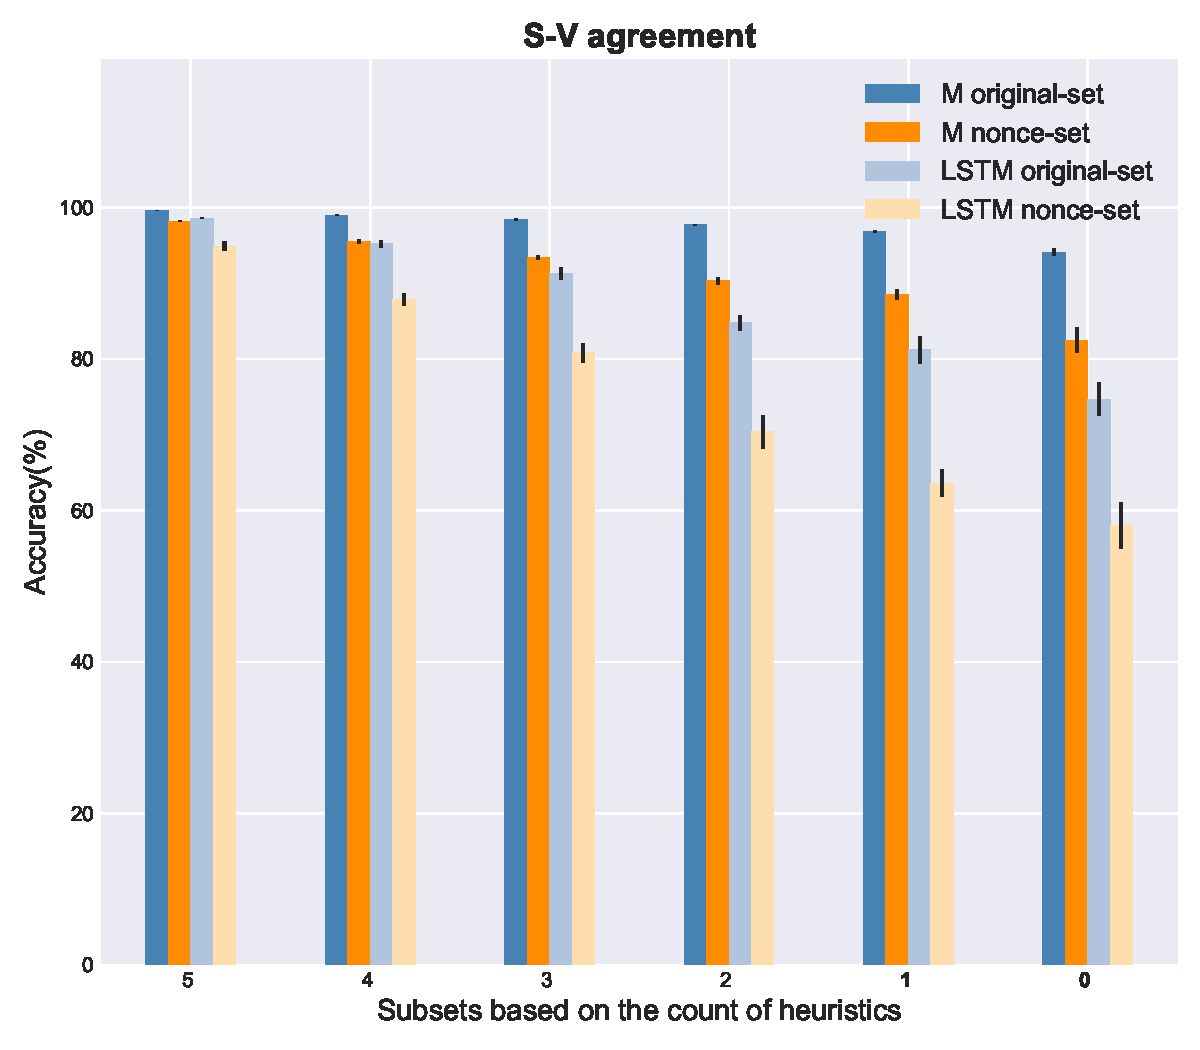
\includegraphics[width=\columnwidth]{figures/nonce_S-V.pdf}}
\scalebox{.85}{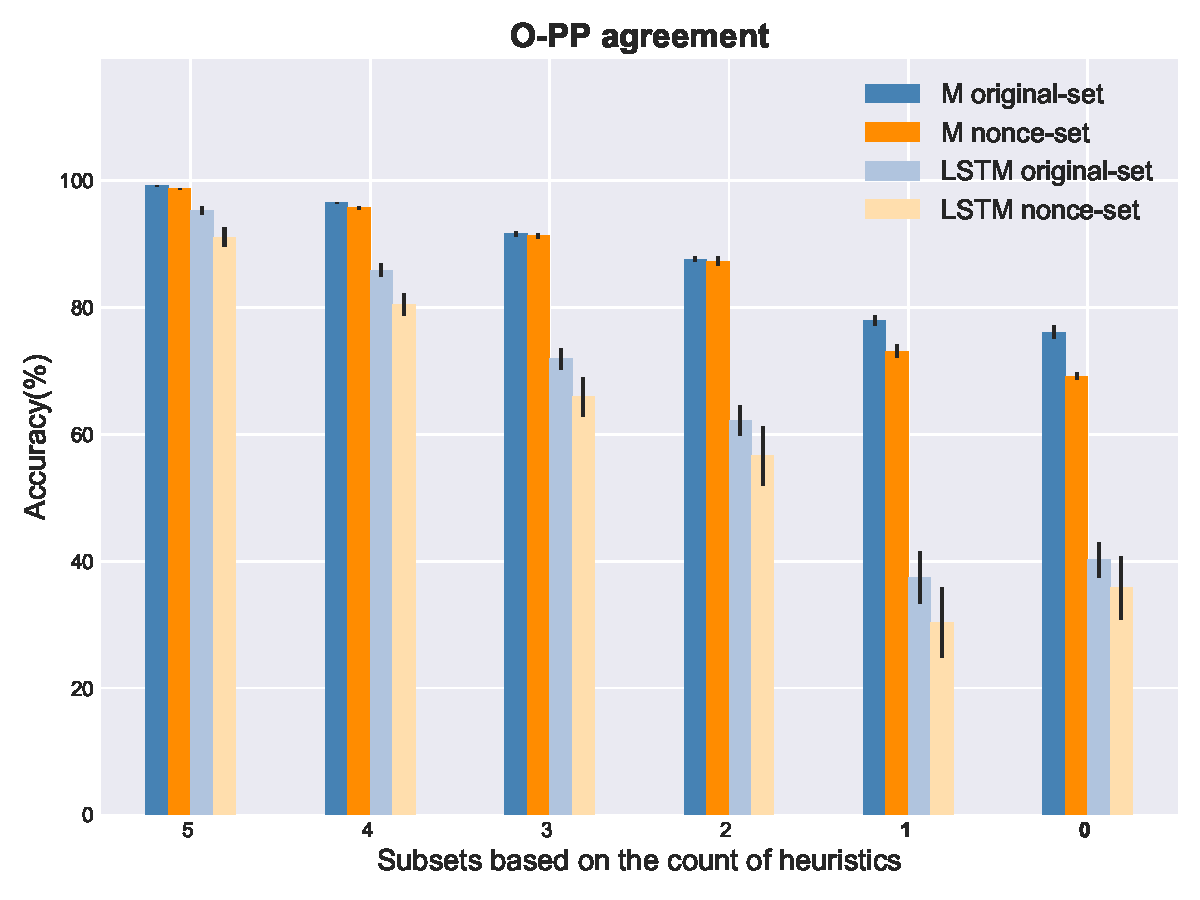
\includegraphics[width=\columnwidth]{figures/nonce_O-PP.pdf}}
\caption{Average accuracy of LSTM (indicated by lighter color bars) and Transformer models on 
 the \textit{Nonce set}, represented by orange bars, and the \textit{Original set}, indicated by blue bars.} \label{fig:nonce_heuristics}
\end{figure} 

Using the evaluation metric described in Section (\textsection\ref{sec:h_eval_protocol}), we also evaluate the syntactic abilities of the models in the \textbf{Nonce} set for the same number agreement tasks. Figure~\ref{fig:nonce_heuristics} reports models performance on the \textbf{Nonce} set compared to the original set. Overall, both architectures exhibit only a mild degradation in accuracy relative to
the \emph{original} setting across the two agreement tasks. Interestingly, the extent of performance degradation seems to correlate with the complexity of the agreement prediction task. As sentences become more abstract, semantic cues appear to have a greater impact on model decisions. Specifically, for the most challenging S-V agreement subset, the Transformer's accuracy drops by 11.6 percentage points, while the LSTM's drops by 16.7 points. For the most difficult O-PP agreement subset, 
the declines are 6.9 and 4.4 points for the Transformer and LSTM, respectively.\footnote{For detailed scores, please refer to Table~\ref{tab:nonce_heuristics} in the Appendix.} Across both agreement tasks, the observed drops in accuracy are similar in scale to what has been reported in prior studies by \cite{gulordava-etal-2018-colorless} and \cite{goldberg19assessing}, suggesting that semantic or collocational confounds have only a moderate impact on our models' performance in agreement prediction tasks.\footnote{See Section~\ref{app:lexical_freq_analysis} in the Appendix for an analysis on lexical variation in the results.}  It further implies that our models primarily rely on syntactic information to determine the correct form of the verb.


\subsubsection{Experiment 2: Impact of frequency effects} %Singular-plural asymmetry} 
\label{sec:freq_effects}

In French, as in many other languages, there is a considerable frequency disparity between singular and plural verbs. In written French, singular third-person verbs are observed to be five to ten times more common than their plural equivalents~\citep{aagren2013input}. Such frequency effects, which can influence various levels of human language processing \citep{marantz2013words}, tend to reduce errors when higher-frequency forms are the target and induce errors when a competing lower-frequency form is the target~\citep{ambridge2015ubiquity}. Empirical studies on agreement tasks involving human subjects reflect this trend. For instance, \cite{villata2017intervention} observed that French speakers tend to produce more correct agreement for the O-PP agreement when the target is singular. This trend is often attributed to human's general bias towards the production of default singular forms \citep{greenberg1963some,corbett2000gender}. These findings prompt us to investigate further: Do neural language models exhibit similar biases as humans in number agreement tasks? To what extent are the decisions made by these models a reflection of the frequency distributions encountered during training?


\begin{table}[ht]
\centering
  \begin{tabular}{l cc cc cc cc}
    \toprule 
    & \multicolumn{4}{c}{S-V} &  \multicolumn{4}{c}{O-PP}\\
    \cline{2-4}  \cline{6-8} 
    & \makecell{Singular} & \phantom{\fontsize{9}{11}\selectfont a} &
    \makecell{Plural}  & &\makecell{Singular} & \phantom{\fontsize{9}{11}\selectfont a} &
    \makecell{Plural}& \\
    \midrule  
    Transformer       & 99.4$_{\pm 0.05 }$ && 97.8$_{\pm 0.1}$ & & 99.2$_{\pm 0.1 }$ && 86.2$_{\pm 0.4}$\\
    
    LSTM        & 98.0$_{\pm 0.3}$ && 85.9$_{\pm 1.5}$ & & 95.4$_{\pm 0.7}$ && 57.2$_{\pm 2.9}$\\
    
    Argmax$_v$(target)        & 99.3$_{\pm 0.0}$ && 0.5$_{\pm 0.0}$ & & 93.2$_{\pm 0.0}$ && 8.6$_{\pm 0.0}$\\
    \bottomrule 
  \end{tabular}
\caption{Accuracy breakdown based on the grammatical number of the \target. The baseline \texttt{argmax$_v$(target)} consistently predicts the more frequently observed number of the \target. \label{tab:results_sing_plur}}
\end{table}

\begin{figure}[ht]
        \centering
        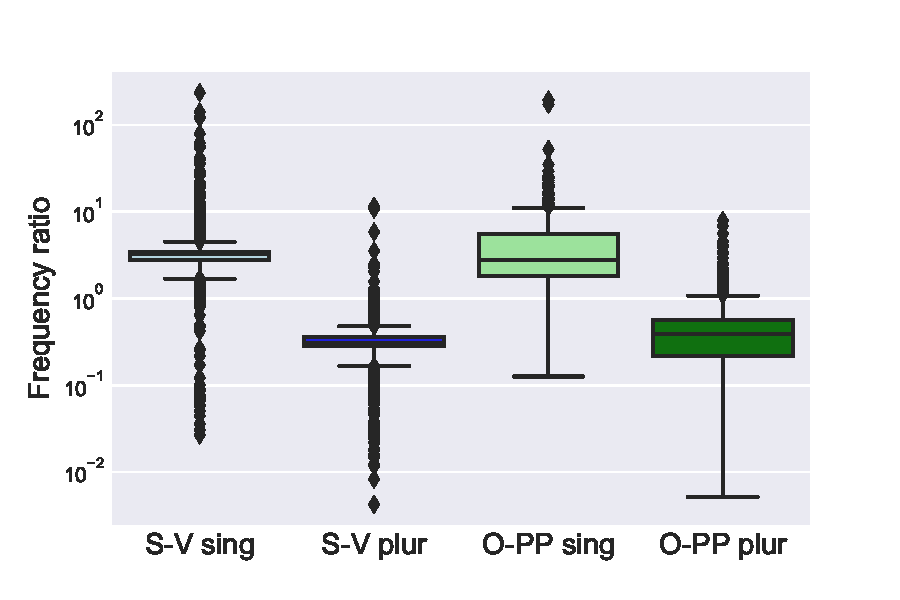
\includegraphics[width=\textwidth]{figures/rel_freq_s-v_o-pp.pdf}
        \caption{Frequency ratio of target form to competing form. For instance, for the \textit{S-V sing} condition, a ratio of $10^1$ indicates that the target verb form (singular) occurs 10 times more frequently in the pretraining data than its competing form (plural). 
        \label{fig:rel_freq}}
\end{figure}


As shown in Table~\ref{tab:results_sing_plur}, our further breakdown of the experimental results in Section~\ref{sec:heuristics} reveals consistent trends across both agreement tasks.
Transformer and LSTM achieve over 95\% accuracy in singular conditions, but show consistent lower performance in plural conditions, suggesting a model bias towards singular forms under our current evaluation metric. Additionally, this performance disparity correlates with the frequency ratio of the target form to the competing form in the pre-training data, as shown in Figure~\ref{fig:rel_freq}. This echoes the findings of \cite{ambridge2015ubiquity} that higher-frequency forms as targets tend to reduce errors. Interestingly, even though the frequency ratios for the singular class in S-V and O-PP agreements are similar, and a similar trend exists for plurals across both tasks (Figure~\ref{fig:rel_freq}), the performance gap between the plural and its corresponding singular is less pronounced in S-V agreement than in O-PP agreement (Table~\ref{tab:results_sing_plur}).


\begin{figure}[ht]
    \centering
        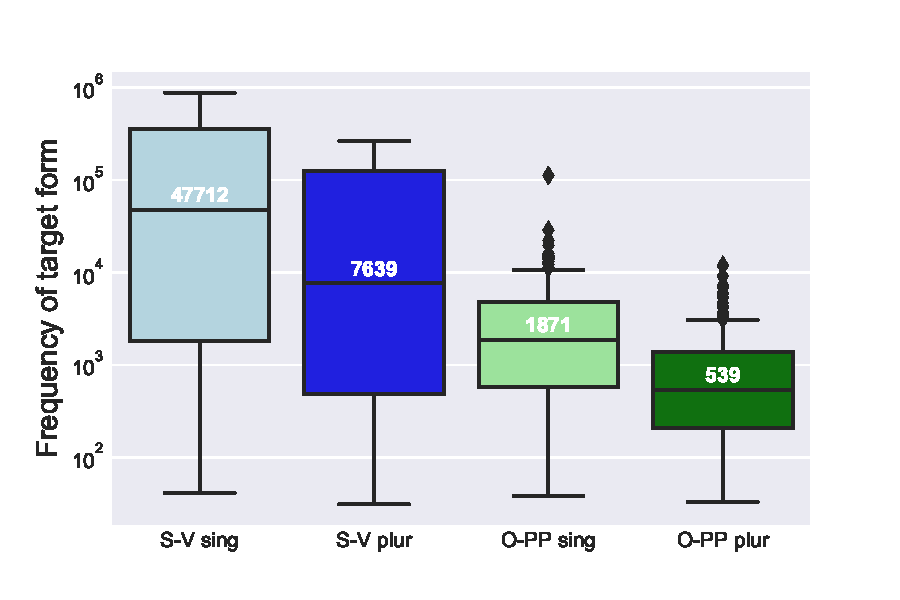
\includegraphics[width=\textwidth]{figures/abs_freq_s-v_o-pp.pdf}
        \caption{Absolute frequency of \target verbs in pre-training data, with medians displayed in white numbers}
        \label{fig:abs_freq} 
\end{figure}

In the case of S-V agreement, the Transformer model shows only a minor drop of 1.6 percentage points in accuracy for plural conditions, compared to the near-perfect accuracy with singular forms. This contrasts sharply with the near-zero accuracy of the heuristic baseline, demonstrating the Transformer's consistent preference for less frequent but grammatically correct verb forms over more frequently occurring forms. These results suggest that Transformer generally applies the subject-verb agreement rules with high accuracy, even when faced with a strong frequency bias. 

In contrast, the models' performance in O-PP agreement exhibits a significant difference between singular and plural conditions. Specifically, Transformer models experience a 13\% drop in accuracy for plural forms, while LSTMs see a more substantial decrease of over 38\%. This suggests that both types of model struggle more with plural forms in O-PP agreement compared to S-V agreement.
 Given that the O-PP agreement is a relatively rare syntactic phenomenon compared to the S-V agreement, as discussed in \S\ref{sec:h_eval_protocol}, this could partially explain the lower overall accuracy of the model in the former task. Additionally, we observe a marked discrepancy in the absolute frequency of \target verbs between S-V agreement and O-PP agreement. As depicted in Figure~\ref{fig:abs_freq}, target verbs in S-V agreement are much more frequent in models' pretraining data compared to those in O-PP agreement. For plural forms, our results align with \cite{wei-etal-2021-frequency}, indicating that more frequent target verbs are more likely to be correctly inflected in number agreement tasks. This is consistent with the frequency effects observed in human language processing. However, for singular forms, despite the absolute training frequency discrepancy of \target forms across the two agreement tasks, models show equivalently high performance on singular conditions for both tasks.  
 This suggests that, similar to humans, neural language models, may also default to using singular forms when handling number agreement tasks in French, corroborating previous research on default reasoning in language models~\citep{jumelet-etal-2019-analysing}. Notably, the Transformer model appears to be capable of effectively leveraging syntactic structures to override this default reasoning in plural conditions, as evidenced by its strong performance in both singular and plural agreement tasks.

While frequency effects could partially account for the observed asymmetry between singular and plural, task complexity also appears to play a significant role in models' lower performance in plural conditions. Further analysis of our evaluation sets reveals a consistent correlation between class distribution and task difficulty (measured by the count of heuristics; \textsection\ref{sec:h_eval_protocol}). In the easiest cases, where any of the five heuristics can solve the task (\emph{5-heuristic} subset), singular target forms predominate, accounting for 94\% of the cases in O-PP agreement and 91\% in S-V agreement. In contrast, in the most challenging cases where no heuristic allows to predict the agreement (\emph{0-heuristic} subset), the plural class becomes the dominant category (O-PP: 99\%, S-V: 96\%). This correlation holds true for both O-PP and S-V agreement. It suggests that in natural corpora, plural verbs tend to appear in more complex and potentially confounding long-distance agreement contexts compared to their singular counterparts. This further explains the models' lower performance in plural conditions. The reasons behind this empirical observation remain elusive. We intend to delve deeper into its implications in future research, using controlled experiments that account for syntactic complexity and class balance.

In summary, our analysis reveals that both Transformer and LSTM models consistently exhibit better performance in singular conditions than in plural ones across two agreement tasks. This trend suggests that these models might possess a frequency-driven bias in number agreement tasks, similar to that observed in humans. Notably, the Transformer model is better at mitigating this singular bias when processing plural conditions, highlighting its ability to leverage syntactic structures. The observed performance asymmetry could arise from several factors, including the higher frequency of singular verbs in the French language, the imbalanced distribution of grammatical number among syntactic constructions of varying complexity, and potential distinctions in how the models encode singularity and plurality, as suggested by \cite{jumelet-etal-2019-analysing}. 

\subsubsection{Experiment 3: Top-k evaluation metric} \label{sec:topK_metric}
%\paragraph{Evaluation metric} 
The evaluation metric we have adopted, which aligns with common practices in the literature  (\S\ref{chp:NA_tasks}), may introduce its own set of biases into our assessment. Specifically, our metric focuses on the model's ability to discriminate between the singular and plural forms of a target verb that naturally occur in a corpus. This approach does not necessarily capture the model's ability to generate a verb form that is both contextually appropriate and correctly inflected for number. This limitation has been noted in previous work, such as the study by \cite{newman-etal-2021-refining}, which observed that language models perform better on verbs they predict to be contextually likely. These considerations raise an important question regarding whether our evaluation metric faithfully reflects the models' likely behavior. In other words, do the most likely words, predicted by the models given a sentence prefix, exhibit consistent agreement features as those obtained from our \textit{target verb} evaluation metric?



To address this question, we propose an alternative evaluation metric, referred to as the $top$-3 evaluation metric, to better measure models likely behavior. Instead of comparing the probabilities of two forms given an evaluation sentence prefix, we focus on the words the models consider most likely to occur. Specifically, we sample the top ten most probable word predictions made by the models for a given sentence prefix. From these words, we use the morphologizer of a pre-trained French model in \textit{spaCy}~\citep{spacy},\footnote{\url{https://spacy.io/models/fr}, we used the model: \textit{fr\_dep\_news\_trf}} to get the three most probable verbs. We then consider the majority number expressed among these three verbs as the models' agreement prediction for that sentence. To ensure a fair comparison between our initial evaluation metric and this $top$-3 evaluation metric, we exclude sentences where the top ten most probable word predictions from the models do not contain any verbs.\footnote{For the Transformer model, we excluded 7.9\% (resp. 29.8\% for LSTM) of the total evaluation sentences (27,582) in the S-V agreement. Similarly, in the O-PP agreement task,  0.3\% of the total evaluation sentences (68,497) were excluded for the Transformer, compared to 45.7\% for the LSTM. Among the excluded sentences, the top ten LSTM predictions are mainly punctuation, prepositions, articles, or nouns. }
 % (resp. LSTM)
\begin{figure}[ht]
    \centering
    \begin{subfigure}[b]{0.49\textwidth}
        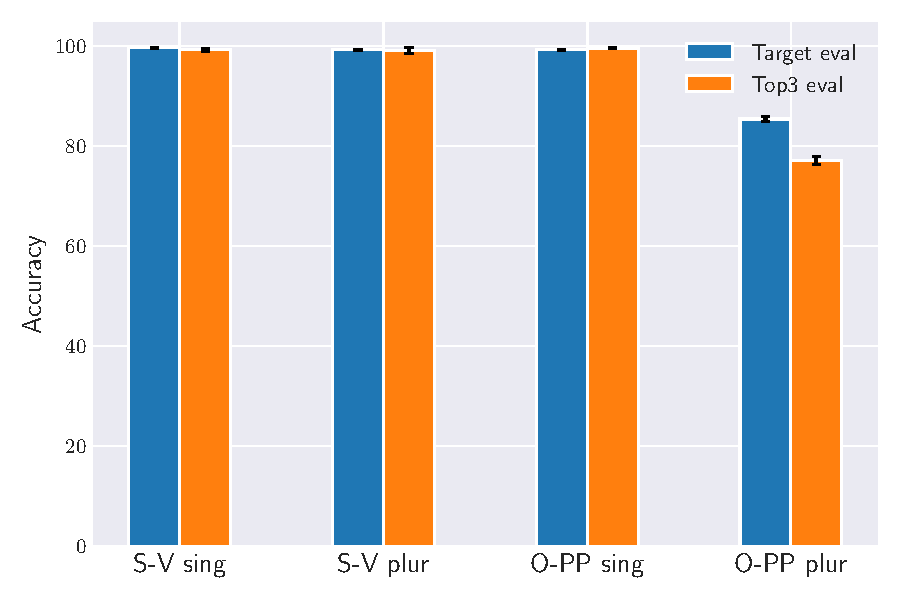
\includegraphics[width=\textwidth]{figures/tm_2_eval.pdf}
        \caption{ \textbf{Transformer} language model}
        \label{fig:tm_2_eval}
    \end{subfigure}
    \hfill
    \begin{subfigure}[b]{0.49\textwidth}
        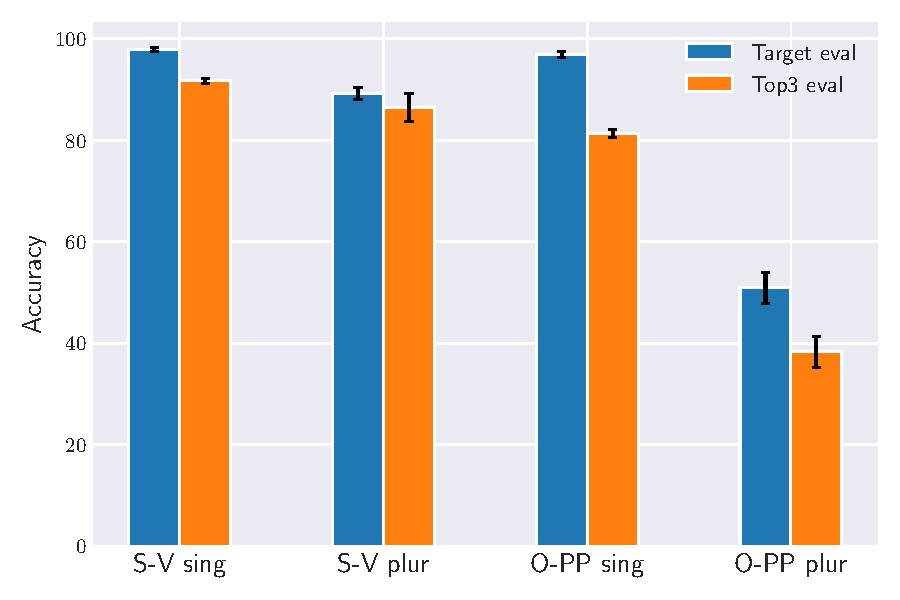
\includegraphics[width=\textwidth]{figures/lstm_2_eval.pdf}
        \caption{ \textbf{LSTM} language model
        }
        \label{fig:lstm_2_eval}
    \end{subfigure}
    \caption{Comparison of models' accuracy in two agreement tasks using $top$-3 evaluation metric (orange bars) and \textit{target verb} evaluation metric (blue bars).}
\end{figure}


As shown in Figures~\ref{fig:tm_2_eval} and~\ref{fig:lstm_2_eval}, the trends observed with the $top$-3 evaluation metric closely align with those of the \textit{target verb} evaluation metric. For both Transformer and LSTM, the two metrics demonstrate a persistent performance asymmetry between singular and plural conditions in both agreement tasks. The performance breakdown based on task difficulty (Table~\ref{tab:tm_full_2_eval} and \ref{tab:lstm_full_2_eval} in the Appendix) also indicates that all models performance decrease with the task difficulty. Notably, for the Transformer, a high level of consistency is observed between the two metrics, with an inter-agreement rate surpassing 92\% in both tasks (see Table~\ref{tab:inter_agreement} in the Appendix for full results).

For the Transformer model, the two evaluation metrics yield similar scores for the S-V agreement and the singular condition of O-PP agreement. However, a decrease of 8.3\% is observed in the plural condition of the O-PP agreement when using the $top$-3 metric. This decrease may be partially attributed to the presence of part-of-speech ambiguous words (e.g., ``données" can be both a noun and a verb) or number ambiguous words (e.g., ``appris" can be both a singular and plural form). In contrast, the strong baseline model, LSTM, consistently exhibits lower accuracy across the board when evaluated with the $top$-3 metric. Additionally, for both agreement tasks, over 29\% of the top ten predictions of LSTM (compared to less than 8\% for Transformers) do not contain any verbs. This finding indicates that the Transformer model demonstrates similar behavior under the two evaluation metrics and exhibits more robust syntactic behavior compared to the baseline LSTM model.

Given the similar performance trends of the Transformer on both agreement tasks across two evaluation metrics, we consider the differences between these metrics minor enough to proceed with the main objective of our study: investigating how the Transformer LM represents syntactic structures when handling two superficially similar long-distance agreement phenomena. Additionally, we want to avoid the potential noise introduced by the $top$-3 evaluation metric, which relies on a pre-trained model to predict morphological features. 
Therefore, all subsequent experiments are conducted using the \emph{target verb} evaluation metric, aligning with the common practice in the literature (\S\ref{chp:NA_tasks}).


Interestingly, our findings based on naturalistic corpora diverge from the observations of \cite{newman-etal-2021-refining}. While their study, using synthetic data, suggests that models perform better on verbs predicted to be the most likely in context, we did not observe this improvement in our study. Future research could further investigate the contributing factors to the observed performance asymmetry between singular and plural forms. This could involve artificially manipulating the relative frequency of singular and plural nouns within different constructions in the model's training data to better understand their influence on performance.


\subsection{Conclusion}
In this section, we evaluated the autoregressive Transformer's ability to process two syntax-sensitive phenomena in French, using number agreement tasks. Our initial experiments demonstrate strong overall performance for both types of agreement, indicating that the model's behavior aligns closely with human language use. Furthermore, we investigated the impact of surface heuristics and other known confounding factors on the model's performance. These findings lend further support to existing research (Section \ref{sec:review_structure_nlm}), confirming that the Transformer model exhibits a robust capability to capture and generalize syntactic information beyond surface heuristics and semantic or collocational cues. 

We observed that while the Transformer does show some sensitivity to frequency effects, it generally displays a consistent preference for grammatically correct forms, effectively overcoming strong biases present in the training data. Compared to the LSTM, a strong baseline in the literature for evaluating syntactic abilities of NLMs (\S\ref{chp:NA_tasks}), the Transformer is less influenced by surface heuristics and frequency effects, and exhibits more consistent performance under different evaluation metrics. These findings suggest that the Transformer meets the first criterion --- behavioral-level similarity --- for genuine syntactic generalization.

Additionally, it is important to recognize that humans also make agreement errors~\citep{BOCK199145}, and also display a bias favoring singular forms, leading to fewer agreement errors for these forms in French object-past participle agreement tasks, as observed by ~\cite{villata2017intervention}. In this context, the heuristics that affect the model's performance might hold relevance not just for the domain of artificial neural networks, but could also offer valuable insights into the study of human linguistic abilities. Specifically, these heuristics could stimulate the development of testable hypotheses for experiments aimed at understanding human syntactic performance. Our heuristic-based approach for crafting evaluation sets could help to build stimuli that effectively measure human capacity for rule-based linguistic generalization.


\section{Locating syntactic information in Transformer language model} \label{sec:probing_location}

The experiments presented in the previous section demonstrate that the Transformer language model consistently outperforms the strong baseline model, LSTM, in long-range subject-verb and object-past participle agreements. Crucially, Transformer is able to abstract away from potential confounds such as lexical co-occurrences or superficial heuristics. This successful behavioral assessment allows us to delve deeper to evaluate the Transformer's representational adequacy as a model that helps to explain human syntactic processing.
In light of this success, which aligns with prior research indicating that Transformers capture a “substantial amount” of syntactic information (\S\ref{sec:review_structure_nlm}), two questions emerge naturally: First, where is this syntactic information located within the Transformer's internal representations? Second, given the superficial similarities between the two types of agreement tasks we studied, does the Transformer model use a uniform internal representation for both, or are there distinct representations that reflect the theoretical nuances of each task?


In this section, focusing on Transformer LM, we investigate the question of \textbf{where} syntactic information is encoded from two perspectives.\footnote{Datasets and code: \url{https://gitlab.huma-num.fr/bli/syntactic-info-distribution}} First, in Section~\ref{sec:within_sentences}, we use probing classifiers, detailed earlier in Section~\ref{sec:probing}, to identify token positions where the agreement information is encoded within the model's internal representation. 
This analysis enables us to localize the agreement feature across token representations within a sentence. Second, in Section~\ref{sec:within_repr}, we use a feature selection method associated with probing to identify the specific subspace within the Transformer's representations that encodes the relevant agreement information.
 

\subsection{Distribution of syntactic agreement information across token positions}\label{sec:within_sentences}
In this section, we investigate where the Transformer encodes the syntactic information necessary for predicting the correct \emph{target} form in the two types of agreement tasks. Specifically, we explore whether this agreement information is distributed across all tokens following the \emph{cue} in the sentence, as theoretically allowed by the self-attention mechanism and observed by \cite{klafka-ettinger-2020-spying}. Alternatively, is this information encoded more locally, centered around the \cue and \target tokens, as predicted by the specific agreement rules?

To investigate these hypotheses, we use probing classifiers following the approach of \cite{giulianelli-etal-2018-hood} (\S\ref{chp:NA_tasks}). In our study, 
 we denote the representation generated by a Transformer LM for the token $t$ at layer $l$ by:
 \begin{equation}
 r_t = \text{Transformer}_l(t) 
 \end{equation}
 Given an evaluation sentence, our goal is to examine whether the representation of a token $t$ within the sentence contains the relevant syntactic agreement feature, denoted as $\mathcal{A}$, which corresponds to the number of the \cue (either `Singular' or `Plural'). To achieve this, we train a classifier defined as a function $\mathcal{C}$ that maps the representation of each token to the agreement feature of the sentence, $\mathcal{A}$:
\begin{equation}
\mathcal{C}:r_t \leadsto \mathcal{A}, \text{with } \mathcal{A} \in \{\text{Singular}, \text{Plural}\}
\end{equation}



The core assumption underlying this approach is that if the Transformer has encoded syntactic agreement information within its representation space, then a probing classifier should be able to ``extract'' this information from the corresponding token representations produced by the Transformer (\S\ref{sec:probing}). 
In this study, we use a logistic regression classifier,\footnote{This choice follows the recommendation of ~\cite{hewitt-liang-2019-designing}, who found that non-linear probes tend to memorize the probing task by leveraging surface pattern recognition, rather than relying on the information captured in the representations of the probed model.} defined as:
\begin{equation}
 \sigma(\theta^T r_t + b) \leadsto \mathcal{A}, \text{with } r_t \in \mathbb{R}^{768} 
\end{equation}
Here, $r_t$ is the token representation extracted from the Transformer's last layer (i.e., the 16th layer in our experiments) for the token $t$, $\sigma$ denoting the sigmoid function. The parameters vector (i.e., coefficients) is represented by $\theta$, and $b$ represents the bias term. 

 \begin{figure}[htbp]
  \centering
  \pgfsetlayers{depgroups,main}
 \scalebox{0.86}{\begin{dependency}
    \tikzstyle{POS}=[font=\fontsize{10}{12}\selectfont]
    %\tikzset{POS/.style={font=\fontsize{9}{11}\selectfont}}
    \depstyle{pref}{draw=blue, fill=blue!25}
    \depstyle{cont}{draw=yellow, fill=yellow!25}
    \depstyle{suf}{draw=green, fill=green!25}
    
    \begin{deptext}
    Sans \& doute \& ces \& {\bf moments}\& de \& \underline{bonheur} \&  que \& son \& \underline{frère} \& lui \& a \& {\bf donnés}  \_\_ \& \  {\bf resteront} \& ... \\
        |[POS]| No \& |[POS]| doubt \& |[POS]| these \& |[POS]| moments\_Pl \& |[POS]| of \& |[POS]| happiness\_Sg \& |[POS]| that \& |[POS]| his \& |[POS]| brother\_Sg \& |[POS]| (to) him \& |[POS]| has  \& |[POS]| given\_Pl \& |[POS]| will\_stay\_Pl \& ...\\ 
     \&  \&  \& {\bf cue} \&  \&  \&  \& \&  \& \& \& {\bf target}  \&  \&  \\
    \end{deptext}
    \depedge[edge unit distance=1ex]{7}{4}{antecedent}
    \depedge[edge unit distance=.5ex]{12}{7}{object}
    %\depedge[edge unit distance=1ex]{13}{4}{nsubj}
    \wordgroup[pref]{1}{1}{2}{prefix}
    \wordgroup[cont]{1}{3}{11}{context}
    \wordgroup[suf]{1}{13}{14}{suffix}
  \end{dependency}}
  \caption{ For the O-PP agreement, the prefix is highlighted in blue, the context in yellow and the suffix in green.
  \label{fig:probing_zones}}
\end{figure}

% \textcolor{blue}{\bf target-v}

\paragraph{Training} To train the probing classifiers, we construct a training set $\mathcal{D} = \{x^{(i)}, \mathcal{A}^{(i)}\}$ as follows. For each token in the sentences of our evaluation set, we extract its representations from the last layer of the Transformer and associate it with a label $\mathcal{A}^{(i)} \in \{ \textrm{Singular}, \textrm{Plural} \}$ indicating the number of the \cue. Next, as illustrated in Figure~\ref{fig:probing_zones}, we divide each sentence into three parts: 
\begin{itemize}[topsep=0pt,itemsep=-1ex,partopsep=1ex,parsep=1ex]
    \item \emph{prefix}: words before the \cue and its dependent words;
    \item \emph{context}: words from the \cue (and its dependent words) to just before the \target;
    \item \emph{suffix}: words following the \target
\end{itemize}
\noindent We train individual probing classifiers for each category of word within each part of the sentences. This approach allows each classifier to specialize in PoS-specific representations of long-distance agreement information. To ensure fair comparison across sentence parts, we exclude tokens with PoS tags that occur less than 100 times, namely SYM, SCONJ, INTJ, PART, and X. This results in a total of 11 token categories in each sentence part, giving us $11*3$ probing classifiers.

For training and evaluation, we split the examples into 80\% training data and 20\% evaluation data. Each classifier is trained using three different train/test splits.\footnote{All classifiers were implemented with the \texttt{scikit-Learn} library~\cite{scikit-learn}. A grid search with 5-fold cross-validation was performed to select the optimal value of the regularization parameter $C$. The \texttt{max\_iter} parameter was set to 1,000 during the training process. Random\_state = 0, 20 and 42} The averaged results are reported in Table~\ref{res:probing_high_level}, and more detailed results per word category are provided in Figure~\ref{tab:res_per_PoS} of the Appendix.

\begin{table}[ht]
    \centering
  \begin{tabular}{l cc cc c}
    \toprule 
    & \multicolumn{4}{c}{Mean probing Accuracy } \\
    \cline{2-5}
    & \makecell{O-PP agreement \\ } & \phantom{\fontsize{9}{11}\selectfont a} &
    \makecell{S-V agreement} & \phantom{\fontsize{9}{11}\selectfont a}  \\
    \cline{2-2} \cline{4-4} 
    \emph{prefix}        & 58.6\%$_{\pm 0.1}$ && 59.5\%$_{\pm 0.2}$ &\\
    \emph{context}       & 92.3\%$_{\pm 0.2}$ && 93.0\%$_{\pm 0.1}$ \\
    \emph{suffix}       & 73.6\%$_{\pm 0.2}$ && 78.1\%$_{\pm 0.2}$  \\
    \bottomrule 
  \end{tabular}
\caption{Probing results across different sentence parts (see
  Figure \ref{fig:ex_agreement}). The reported scores represent the average accuracy of all PoS-based classifiers for each sentence segment. \label{res:probing_high_level}}
\end{table}

\paragraph{Results} The average accuracy achieved by our probes on different parts of the sentence is presented in Table~\ref{res:probing_high_level}. We observe a similar pattern for both O-PP and S-V agreement: the syntactic agreement information about the number of the \cue is essentially encoded within the tokens of the \emph{context}. It is not distributed across all tokens following the cue in the sentence.

As expected, in both tasks, the probe performance on the \emph{prefix} is very low. Given the autoregressive nature of the model, token representations in the \emph{prefix} cannot attend to the \cue, and thus, cannot encode its number information. The accuracy observed on the \emph{prefix} mainly reflects the difference in prior probabilities of the two grammatical number classes within the evaluation set.\footnote{As discussed in \S\ref{sec:NA_data}, within the two evaluation sets, 65\% of the target past participles in O-PP agreement are singular, while 70\% of the target verbs in S-V agreement are singular.} In contrast, when using tokens from the \emph{context} as input features, the probe accuracy is consistently high for both agreement types. However, the accuracy significantly drops for the \emph{suffix} tokens, though it remains higher than that observed for the \emph{prefix}. This suggests that the information required to predict the correct \emph{target} form is distributed across all tokens between the \emph{cue} (where the number of the \emph{target} verb is specified) and the \emph{target} (where this information is being `used'). This finding, to some extent, challenges the observations of \cite{wisniewski-etal-2021-screening}, who discovered that gender information in a neural translation system is distributed throughout the source and target representations. However, it should be noted that their study focused on a different type of information and was limited to sentences with a simple structure.

 
Results so-far indicate that the agreement information related to \cue is mainly distributed across all tokens in the \emph{context} part of the sentences. To gain a more precise understanding of how the Transformer model tracks this agreement information from \cue to \target, we conduct an experiment that focused on a specific sentence pattern with a fixed six-word \emph{context}. Specifically, we focus on sentences where \cue is
separated from the relative pronoun only by a prepositional
phrase. This pattern applies to sentences such as the one shown in (\ref{ex:S_V_fixed_probing}) for long-distance subject-verb agreement, and (\ref{ex:O_PP_fixed_probing}) for object-past participle agreement.

\begin{exe}
    \ex \label{ex:S_V_fixed_probing}
    \begin{tabular}{lllllllll}
    Sentence: & ... & \textbf{bureau·x} & en & métal & qu' & il & aime & \textbf{coût·ent } ... \\
    & ... & {\scriptsize desks} & {\scriptsize Prep.} & {\scriptsize metal} & {\scriptsize that} & {\scriptsize he} & {\scriptsize loves} & {\scriptsize cost }... \\
    Pattern: & ... & \texttt{Subject} & \texttt{ADP} & \texttt{NOUN} & \texttt{que} & \texttt{PRON} & \texttt{V} & \texttt{target V}...
    \end{tabular}
\end{exe}

\begin{exe}
\ex \label{ex:O_PP_fixed_probing}
\begin{tabular}{lllllllll}
   Sentence: & ... & \textbf{bureau·x} & en & métal & qu' & il & a & \textbf{trouvé·s } ... \\
   & ... & {\scriptsize desks} & {\scriptsize Prep.} & {\scriptsize metal} & {\scriptsize that} & {\scriptsize he} & {\scriptsize has} & {\scriptsize found\_Pl } ... \\
   Pattern: & ... & \texttt{Antecedent} & \texttt{ADP} & \texttt{NOUN} & \texttt{que} & \texttt{PRON} & \texttt{AUX} & \texttt{target PP }...
\end{tabular}
\end{exe}

\paragraph{Training} To examine the distribution of the agreement information between the \emph{cue} and the \emph{target}, we build a dataset for each agreement phenomenon, following the previously defined patterns with a fixed six-word \emph{context}. Each position within the \emph{context} is labeled with the corresponding PoS tag of the tokens, as illustrated in (\ref{ex:S_V_fixed_probing}) and (\ref{ex:O_PP_fixed_probing}). Additionally, we also consider the five tokens before and after the six-word \emph{context} window, denoted as \texttt{$b_i$} (for tokens before) and \texttt{$a_i$} (for tokens after), where \texttt{i} represents the position relative to the pattern, as illustrated by the X-axis labels in Figure~\ref{fig:fix5}.


For the training set, we randomly sample 800 examples for each agreement phenomenon, ensuring a balance between singular and plural forms. For the test set, we sample a balanced set of 200
examples, with 100 sentences where the embedded noun (at the `NOUN' position within the \emph{context}) is an \emph{attractor}, and 100 sentences where this noun has the same number as the \emph{cue}.\footnote{We conducted the sampling process using three different seeds, and for each sampling, we performed three train/test splits. The reported scores are averaged across all splits.} Unlike the previous experiment where we trained probing classifiers on representations of all words in the sentence based on their word categories and their location in the sentence, in this experiment, we train distinct classifiers for each position within the defined scope of sentences.
%, as illustrated by the x-axis labels in Figure~\ref{fig:fix5}.

\begin{figure}[htbp]
    \begin{subfigure}{\textwidth}
        \centering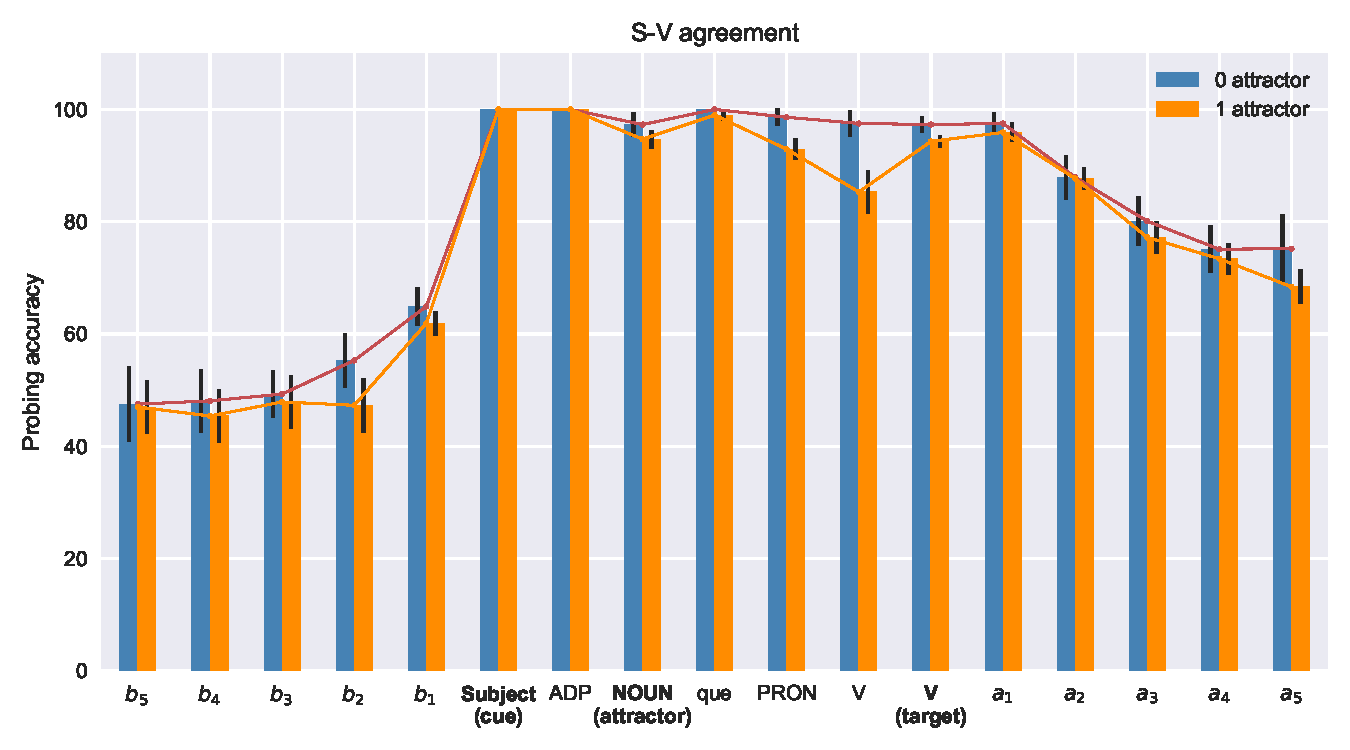
\includegraphics[width=0.95\textwidth]{figures/probing_subj-v.pdf}
    \end{subfigure}
    \vspace{0.2cm}
    \begin{subfigure}{\textwidth}
        \centering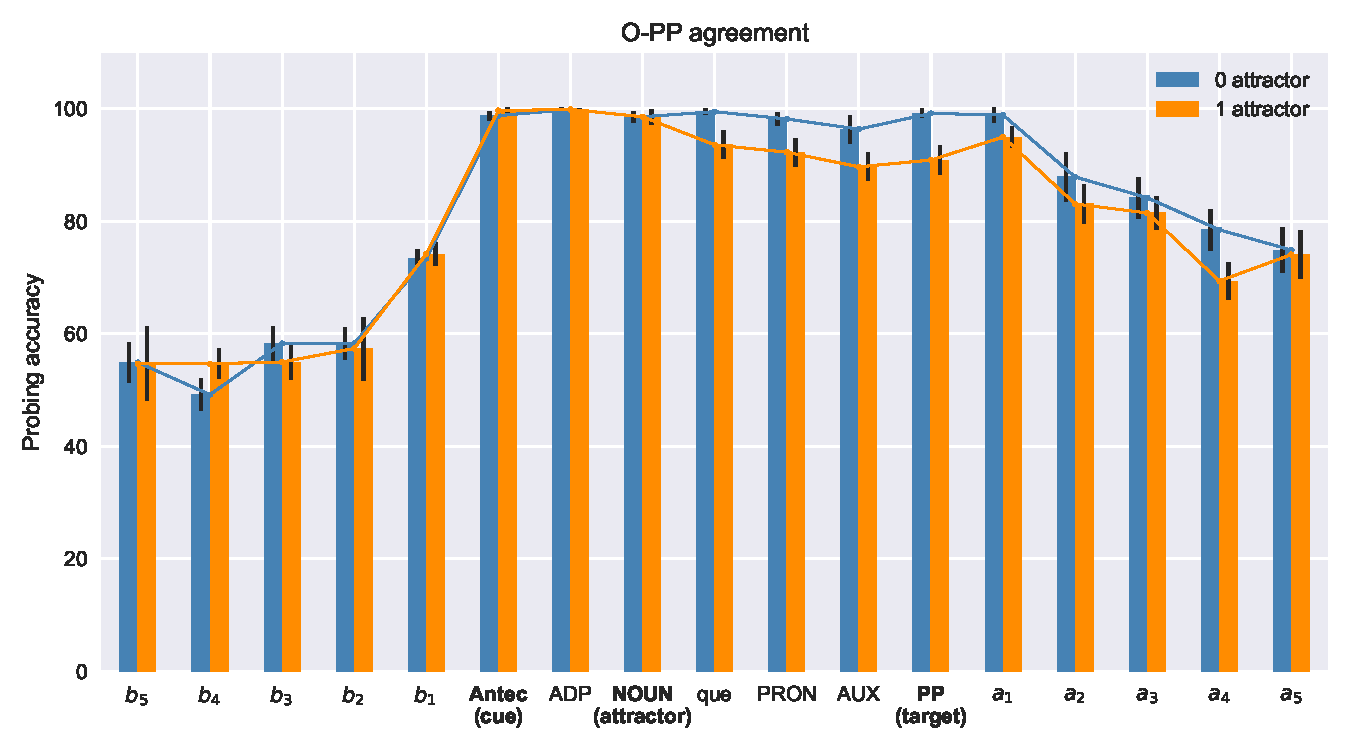
\includegraphics[width=0.95\textwidth]{figures/probing_obj-pp.pdf}
    \end{subfigure}
    \caption{Average probing accuracy at each position based on the number of the
      \emph{cue}. The \texttt{b$_i$} (resp. \texttt{a$_i$}) position
      denotes the $i$-th token before (resp. after) the pattern. The position labeled as `Noun' corresponds to a noun with the opposite number as the \emph{cue} in the 1-attractor subset, and a noun with the same number as the \emph{cue} in the 0-attractor subset.
      \label{fig:fix5}}
\end{figure}

\paragraph{Results} 
We plot in Figure~\ref{fig:fix5} the average probing accuracy at different positions of the specific construction for both agreement phenomena. The results show a consistent pattern: the accuracy of the probes is initially low in the \emph{prefix} (i.e., b-positions) but starts to increase from the position just before the \emph{cue}. This position often corresponds to determiners or adjectives that need to agree in number with the \emph{cue}. As we move into the \emph{context}, the accuracy stabilizes, with probes achieving very high accuracy, even at the attractor position. The accuracy then drops sharply after passing the \emph{target}, especially when an attractor is present in the \emph{context}. It appears that once the \emph{target} has been encountered and the number information of the \emph{cue} is no longer relevant, subsequent tokens no longer encode it. This trend is consistently observed for both types of agreement phenomena. 

Unsurprisingly, the probes achieve perfect scores at and just after the \emph{cue} positions, as well as at the position immediately following the \emph{target}. This suggests that the Transformer has learned to recognize and store the number information of the \emph{cue} and \emph{target} in its internal representations. And this information is encoded in a linearly extractable manner.  

A particularly interesting observation arises when considering the \textit{1-attractor} subset. The accuracy of the probes only slightly degrades at positions immediately following the attractor, which carries the opposite number to the probed grammatical number. Intriguingly, at the target position, where the agreement information from the \emph{cue} is being used, the probe accuracy shows a reboost, in particular in S-V agreement. This suggests that the model appears to know where to pinpoint the syntactic number information, enabling it to avoid potential misleading cues. These observations suggest a coherent and robust flow of agreement information within the Transformer's representations. 


\subsection{Probing internal representations components} \label{sec:within_repr} 
Our previous experiment using probing classifiers revealed that agreement
information is encoded across all tokens within the \emph{context}. In this study, we aim to determine \textbf{where} within the Transformer's representation space this information is encoded. Specifically, we want to identify which components of the token representations generated by the Transformer are most crucial for capturing this syntactic agreement information.

To achieve this, we use an $\ell_1$-regularized logistic regression model,
known for its tendency to produce sparse feature vectors by driving many feature coefficients, denoted by $w_i$ in the equation (\ref{eq:LR_weights}), towards zero \citep{tibshirani96regression,ng2004feature}. This characteristic makes it well-suited for feature selection tasks, allowing us to identify the most relevant components within the Transformer's representations that are responsible for capturing the agreement information.
The $\ell_1$-regularized logistic regression model follows the formulation:
\begin{equation}
\begin{aligned}
\mathbb{P}_{\ivec{w},b}(y=\text{Singular}|x_i) &= \sigma(\ivec{w}^T x_i + b),  \\
\text{where } \ivec{w}^T x_i &= w_1*x_1 + w_2*x_2 + \ldots + w_{768}*x_{768}
\end{aligned}
\label{eq:LR_weights}
\end{equation}
where $\ivec{w}$ represents the parameter (i.e., coefficients) vector, $x_i$ denotes the token representation at position $i$ in a sentence, and $y$ represents the grammatical number of the \cue, which is the agreement information. This model minimizes the objective function with an $\ell_1$ regularization term:
\begin{equation}
    \sum_{i=1}^n -\log P(y_i | \ivec{x}_i;\ivec{w}) + \frac{1}{C}||\ivec{w}||_1
\end{equation}
where, $C$ represents the inverse of regularization strength. As the value of $C$ increases, the number of features with non-zero coefficients $w_i$ also increases. By varying the values of $C$, we can control the sparsity level of the solution $\ivec{w}$, thereby identifying the most relevant components of the Transformer's representations for the probing tasks. 

\begin{figure}[htbp]
  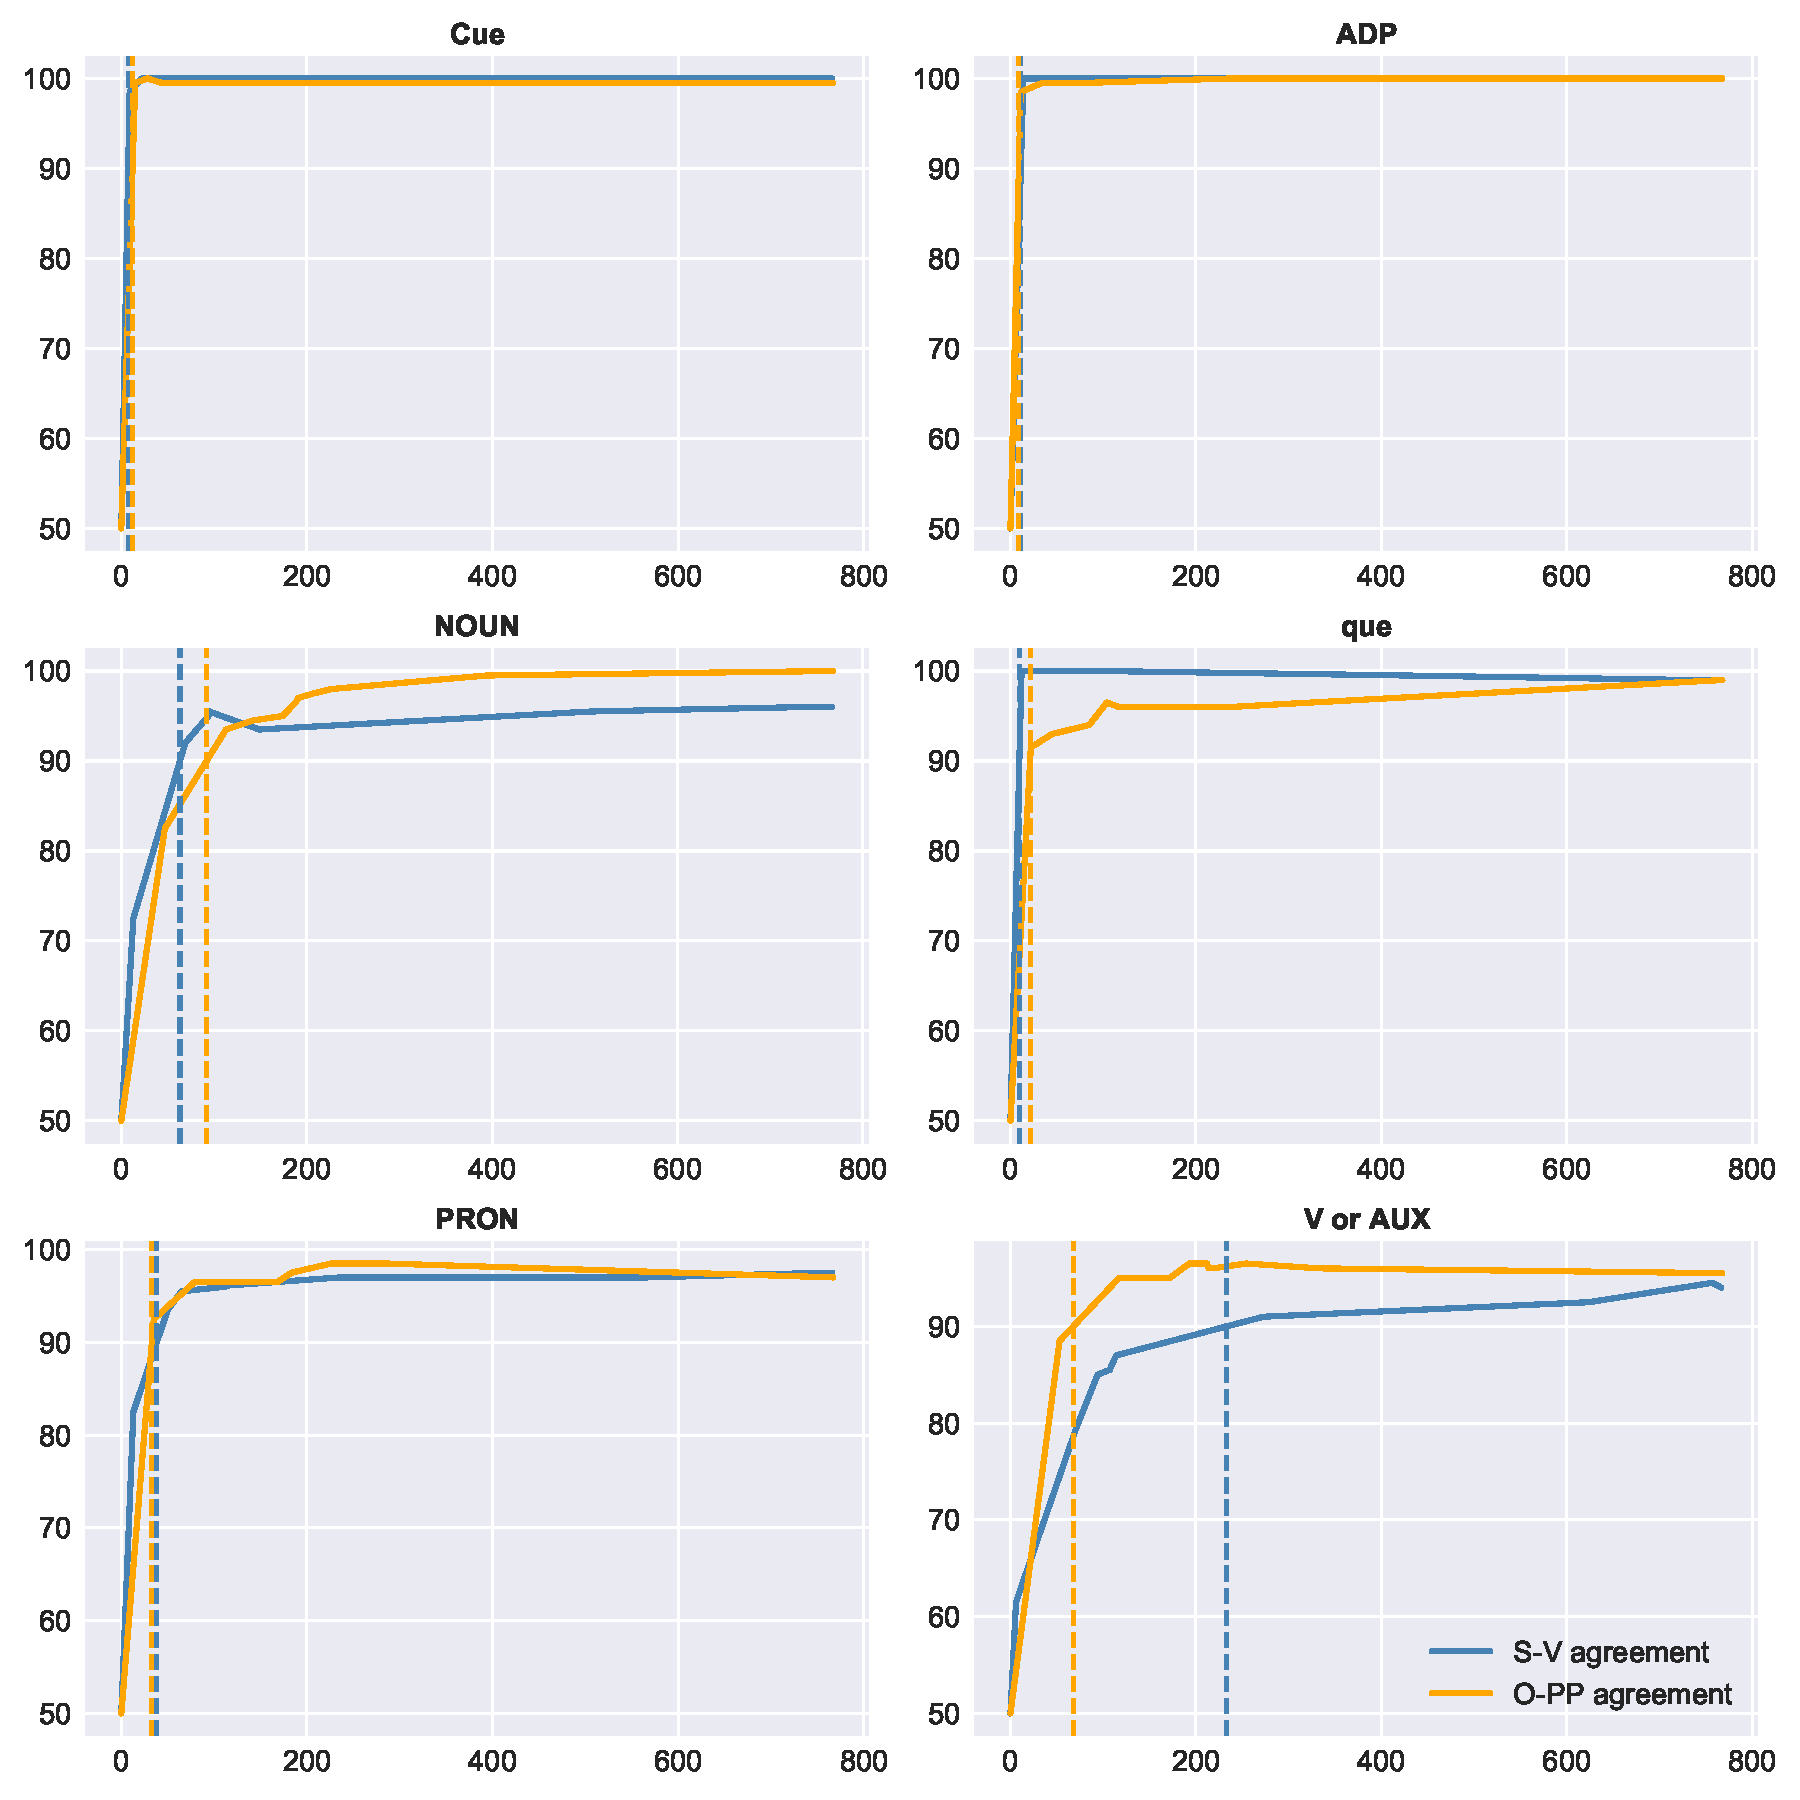
\includegraphics[width=\columnwidth]{figures/probing_c-path.pdf}
  \caption{Probing accuracy as a function of the count of dimensions (for 768-dimension token representations)  with non-zero coefficients, obtained through feature selection using $\ell_1$ regularized logistic regression for each position within \emph{context}.
  The X-axis denotes the count of non-zero coefficient dimensions, and the Y-axis represents probing accuracy. Vertical dashed lines indicate the points at which the accuracy reaches 90\%. 
    \label{fig:res_C_path}}
\end{figure}

\paragraph{Training} In contrast to the previous experiment where we assessed probing accuracy with a fixed optimal regularization parameter $C$, in this study we vary the values of $C$ in the $\ell_1$-regularized logistic model as a means for feature selection. We replicate the same task from Section~\ref{sec:within_sentences}: training a classifier to map token representations to a binary label indicating the grammatical number of the \cue. We use the same training and evaluation dataset: sentences of six-word \emph{context} (\S\ref{sec:within_sentences}). For each position within the \emph{context}, we train a separate classifier (total of six classifiers). We first determine the lowest bound for $C$ such that the feature coefficients are guaranteed to be non-zero.\footnote{We used the \textit{l1\_min\_c} function in scikit-learn~\cite{scikit-learn} to compute this lowest bound.} $C$ is then increased evenly on a log space to decrease the regularization strength. Finally, we compute and plot the \emph{regularization path} of models from most to least regularized.
 

\paragraph{Results} Figure~\ref{fig:res_C_path} reports the regularization path of the probing classifiers for each position within the \emph{context}. It is clear that high probing accuracy can be achieved using only a small number of dimensions in most positions. Remarkably, at the \cue position, the probe can distinguish the grammatical number feature with just one dimension of token representations, reaching over 90\% accuracy for both agreement phenomena. Moreover, 7 out of the top 9 dimensions with the most significant coefficients are shared between the two types of \cue. This observation aligns with the observations of \citep{amini2023naturalistic}, suggesting that the Transformer's representation linearly encodes the grammatical number information of nouns within a few dimensions. We additionally found that for the \texttt{ADP} (immediately following \cue) and \texttt{que} positions, which do not possess inherent grammatical number features, fewer than ten dimensions are required for the probing classifier to achieve an accuracy greater than 90\%. These crucial dimensions differ between the two types of agreement constructions and also vary from one position to another.

Interestingly, even when the most relevant dimensions\footnote{The minimal dimensions that enable the respective probe to achieve over 90\% accuracy.} identified by the feature selection process are removed from these representations, probes trained on the remaining dimensions still achieve over 90\% accuracy. This holds true for both types of agreement phenomena, suggesting that the agreement information is redundantly encoded in the Transformer's representations.



\subsection{Conclusion}

In this section, we explored the encoding and location of syntactic agreement information in a Transformer language model that demonstrates strong overall performance in number agreement tasks (\S\ref{sec:heuristics}). Our probing experiments provided clear evidence of a localized distribution of agreement information within the \emph{context} tokens, even though
the self-attention mechanism theoretically allows this information to spread across all subsequent tokens after the \cue. Additionally, we used a feature selection method to investigate the localization of agreement information within contextualized representations. Our findings reveal that while this information is encoded in a small number of highly correlated dimensions, it is also fuzzily encoded in a redundant way across the remaining dimensions.

 
The results of the probing experiments indicate that the Transformer
language model encodes syntactic agreement information in a very similar way
for both long-range agreements. In terms of acquired
abstractions, the probing methodology does not provide evidence to suggest that the model acquires substantially different representations for
each agreement phenomenon.


\section{Right for the right reason: Exploring mechanisms of agreement computations}\label{sec:causal}

In the previous section, we used probing classifiers to locate the encoding of agreement information, revealing that it is primarily encoded across all token representations between the \cue and the \target. However, probing comes with a notable limitation as outlined by~\cite{belinkov-glass-2019-analysis}: it only reveals a correlation between the representations and the syntactic information measured by the probe, without providing insight into \textbf{whether} and \textbf{how} this information is actually involved in the model's prediction process. Consequently, the validity of conclusions drawn from probing experiments has been a subject of debate (\S\ref{sec:sota_causal_approaches}).

In this section, we take inspiration from more recent work \citeti{elazar2021amnesic,finlayson-etal-2021-causal,ravfogel-etal-2021-counterfactual} that focuses on understanding the causal relationship between the linguistic properties of interest and the model's behavior. We propose a novel causal framework for intervening in the self-attention mechanism to identify which tokens are genuinely responsible for providing the number information used by the model during the agreement resolution process. This not only contributes to our understanding of the model's inner workings but also serves to assess its representational adequacy. Specifically, we aim to examine whether the Transformer's approach to resolving S-V and O-PP agreements aligns with established linguistic theories. In light of its empirical success in behavioral assessment, this theoretical alignment can serve as the second critical requirement for using the Transformer model to offer explanatory insights into human syntactic processing.


This section is structured as follows. First, in Section \ref{sec:causal_framework}, we present the causal framework and define the testable hypotheses. Subsequently, we describe the experimental setup and present the results in section \ref{sec:causal_expe_res}. Finally, we provide an in-depth discussion, analyzing the implications of our findings, and draw conclusions in section \ref{sec:causal_discussion}.

\subsection{The Causal Framework} \label{sec:causal_framework}
This study aims to investigate the causal relationship between the Transformer model's behavior in number agreement tasks and its encoding of agreement information within its representations. Specifically, we seek to understand if the linear encoding of agreement information within the \emph{context}, as revealed by the probing classifiers (\S\ref{sec:probing_location}), causally affects the Transformer's prediction for NA tasks. To address this question, we propose a causal framework inspired by the theory of causal inference~\citep{pearl2018book}. Central to our approach is the concept of causal interventions, where we modify the state of a specific variable --- in this case, the encoding function to compute the token representation for the \target\ --- to observe the resulting effects on the system's behavior. This methodology allows us to explore counterfactual scenarios: How would the Transformer's behavior change if it were deprived of access to certain token representations, and consequently, the agreement information encoded within them? By answering this counterfactual question, we can measure the usefulness of specific information to the model's prediction and compare how the Transformer actually uses this encoded information in handling both types of agreement. 

\paragraph{Causal intervention on self-attention computation}
Transformers rely on self-attention mechanism to build a contextualized representation for each token by
iteratively computing (as a first
approximation) the token representation as a linear combination of
 all previous token representations in the sentence (Figure~\ref{fig:mask_que}). To investigate the causal impact of specific tokens on the model's agreement prediction at the \target position, we propose an analysis method based on causal intervention. This method involves cutting the direct attention from the \target position to the tokens of interest, effectively neutralizing their contribution to the
construction of the \target's representation.  For instance, in Figure~\ref{fig:mask_que}, when the Transformer is predicting the \target verb, the intervention prevents the self-attention from attending to the ``que'' token. This intervention enables us to build a counterfactual representation
for the \emph{target} that does not take into
account the representation of the ``que'' token, thus removing any direct access to the agreement information
encoded in the representation of the neutralized token --- ``que''. This neutralization process thus approximates the do (•) operator in the causal inference literature.  

\begin{figure}[ht]
\centering
\scalebox{0.8}{
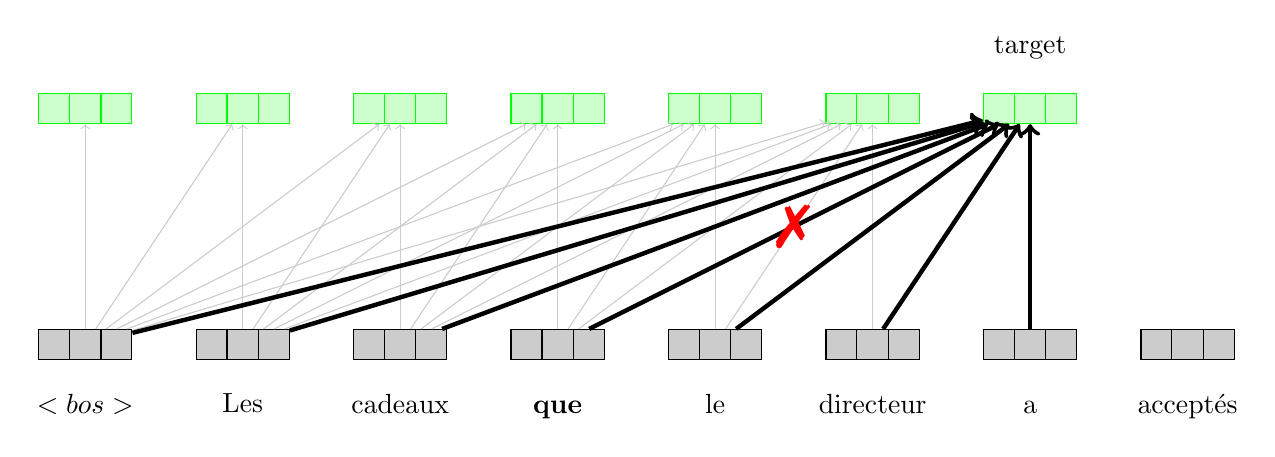
\begin{tikzpicture}[
      neurons/.style 2 args={
        rectangle split,
        rectangle split horizontal,
        draw=#2,
        rectangle split parts=#1,
        fill=#2!20}]
      
 \node[neurons={3}{green}] (s1) at (0,3) {};
 \node[neurons={3}{green}] (s2) at (2,3) {};
 \node[neurons={3}{green}] (s3) at (4,3) {};
 \node[neurons={3}{green}] (s4) at (6,3) {};
 \node[neurons={3}{green}] (s5) at (8,3) {};
 \node[neurons={3}{green}] (s6) at (10,3) {};
 \node[neurons={3}{green}] (s7) at (12,3) {};

\node (o1) [above=5mm of s7.center] {target};

 \node[neurons={3}{black}] (x1) at (0,0) {};
 \node[neurons={3}{black}] (x2) at (2,0) {};
 \node[neurons={3}{black}] (x3) at (4,0) {};
 \node[neurons={3}{black}] (x4) at (6,0) {};
 \node[neurons={3}{black}] (x5) at (8,0) {};
 \node[neurons={3}{black}] (x6) at (10,0) {};
 \node[neurons={3}{black}] (x7) at (12,0) {};
 \node[neurons={3}{black}] (x8) at (14,0) {};

  \node (w1) [below=5mm of x1.center] {$<bos>$};
 \node (w2) [below=5mm of x2.center] {Les};
 \node (w3) [below=5mm of x3.center] {cadeaux};
 \node (w4) [below=6mm of x4.center] {\bf que};
 \node (w5) [below=5mm of x5.center] {le};
  \node (w6) [below=5mm of x6.center] {directeur};
 \node (w7) [below=6mm of x7.center] {a};
 \node (w8) [below=5mm of x8.center] {acceptés};

\draw [->, color=gray!40] (x1) -- (s1);


\draw [->,color=gray!40] (x1) -- (s2);
\draw [->,color=gray!40] (x2) -- (s2);


\draw [->,color=gray!40] (x1) -- (s3);
\draw [->,color=gray!40] (x2) -- (s3);
\draw [->,color=gray!40] (x3) -- (s3);

\draw [->,color=gray!40] (x1) -- (s4);
\draw [->,color=gray!40] (x2) -- (s4);
\draw [->,color=gray!40] (x3) -- (s4);
\draw [->,color=gray!40] (x4) -- (s4);

\draw [->,color=gray!40] (x1) -- (s5);
\draw [->,color=gray!40] (x2) -- (s5);
\draw [->,color=gray!40] (x3) -- (s5);
\draw [->,color=gray!40] (x4) -- (s5);
\draw [->,color=gray!40] (x5) -- (s5);

\draw [->,color=gray!40] (x1) -- (s6);
\draw [->,color=gray!40] (x2) -- (s6);
\draw [->,color=gray!40] (x3) -- (s6);
\draw [->,color=gray!40] (x4) -- (s6);
\draw [->,color=gray!40] (x5) -- (s6);
\draw [->,color=gray!40] (x6) -- (s6);

\draw [->,ultra thick] (x1) -- (s7);
\draw [->,ultra thick] (x2) -- (s7);
\draw [->,ultra thick] (x3) -- (s7);
\draw [->,ultra thick,ban] (x4) -- (s7);
\draw [->,ultra thick] (x5) -- (s7);
\draw [->,ultra thick] (x6) -- (s7);
\draw [->,ultra thick] (x7) -- (s7);
\end{tikzpicture}
}
\caption{With the initial masked self-attention mechanism, the next token representation is computed as a weighted sum of all previous token representations. To assess the impact of ``que'' on the model's agreement behavior, the causal intervention involves cutting the direct attention from the \target position to the token ``que'' (denoted by~\textcolor{red}{\ding{55}}), and then comparing the Transformer's prediction before and after this intervention.}\label{fig:mask_que}
\end{figure}


By comparing the model's prediction on the agreement tasks before and after different interventions, we can assess whether the representations of one or
several specific token(s) have a direct impact on the model's behavior. Table~\ref{ex:mask_que} provides an example from our evaluation set, highlighting the effect of an intervention targeting the token ``que''. As the intervention occurs only when the target verb is
being predicted, there is no impact on the tokens preceding it (i.e., no changes in log probabilities have been observed up to the \target). In this example, the Transformer originally assigned a higher
probability to the correct plural form ``accepté·s'' than to the
incorrect singular form ``accepté''. However, after the intervention, the
situation is reversed, and the model prefers the (incorrect) singular
form. This shift indicates that, for this specific sentence, the direct attention to the token ``que'' has a crucial causal impact on the model's agreement behavior.




\begin{table*}[!ht]
  \centering
  \scalebox{0.9}{
  \begin{tabular}{l|ccccccc|c|c}
    \toprule
    \phantom{ab}& <bos> & Les & cadeau\textbf{x} & que& le & directeur& a & accepté·\textbf{s} / accepté* & $\mathcal{A}$\\
    \phantom{ab}& & \scriptsize The\_Pl & \scriptsize gifts\_\bf{Pl} & \scriptsize that & \scriptsize the & \scriptsize director & \scriptsize has & \scriptsize accepted\_\textbf{Pl} / \scriptsize accepted\_Sg* & \\
    \midrule
    Original& &-2.8&-9.5 &-7.3&-1.8&-6.1&-3.9&\textbf{-5.9} / -8.3& 1\\
    Mask `que' &&-2.8&-9.5 &-7.3&-1.8&-6.1&-3.9&-13.7 / \textbf{-11.9}&0 \\

    \bottomrule
  \end{tabular}}
\caption{Comparison of log-probabilities for each token of example sentences processed by our Transformer LM, before and after the intervention on ``que''. Sentences contain either the plural form of the target verb \textit{acceptés}, or its singular form \textit{accepté}. $\mathcal{A}$-column: 1 indicates a predicted agreement feature matching the gold label, 0 indicates no match. 
\label{ex:mask_que}  }
\end{table*}

Specifically, we perform interventions on self-attention  across all layers and heads of our Transformer language model.  
As discussed in Section~\ref{sec:auto_transformer}, the original attention mask matrix, $\textsc{mask} \in \{0, -\infty\}^{n \times n}$, is defined as:
\begin{equation}
\textsc{mask}_{ij} = \begin{cases}
-\infty & \text{if } j > i \\
 0 & \text{otherwise}
 \label{eq:orig_attention_mask}
\end{cases}
\end{equation}
\noindent The mask sets future positions (relative to the current token) to negative infinity and past positions to zero. By adding this mask to raw attention scores before applying the softmax function, future positions get an attention score of 0 --- this is because the softmax of negative infinity is 0. Previous and current positions remain unchanged since adding zero does not alter their raw scores. As a result, we effectively zero out the attention scores for all positions in the future.

To implement our causal interventions, we extend the original attention mask by additionally setting the weights of specific tokens of interest to be zero. For instance, in a sentence where the position of ``que'' is denoted as $q$ and the target position as $t$, we modify the initial attention mask, $\textsc{mask}$, by setting $\textsc{mask}^{l}_{t,q} = -\infty$ across all attention layers and heads. This effectively cuts the direct attention from the \target position to the token ``que'' while keeping the rest of the self-attention mask unchanged, as shown in Figure~\ref{fig:mask_que}. 

We specifically aim to estimate the causal effect of direct attention from \target to specific tokens on the model's behavior. It's worth mentioning that agreement information may not be exclusively conveyed through direct attention; intermediate tokens can also convey relevant details \citep{klafka-ettinger-2020-spying,lasri-etal-2022-probing}. In Figure~\ref{fig:mask_que}, for instance, the intermediate tokens between ``que'' and \target continue to incorporate ``que'' directly into their representations. Since the representation of \target indeed
relies on the representations of all preceding unmasked tokens, the information encoded in ``que'' can still be indirectly considered. 

% formal description
\paragraph{Abstract causal model} We now formalize the causal intervention by defining an abstract causal model as illustrated in Figure~\ref{fig:causal_dag}:

\begin{figure}[ht]
    \centering
    \begin{center}
    \scalebox{0.9}{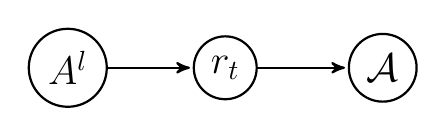
\begin{tikzpicture}[->, >=stealth', shorten >=1pt, auto, node distance=2cm, thick, main node/.style={circle, draw, font=\sffamily\Large\bfseries}]
    \node[main node] (1)  {$A^l$};
    \node[main node] (2) [right of=1] {$r_t$};
    \node[main node] (3) [right of=2] {$\mathcal{A}$};
    
    \path[every node/.style={font=\sffamily\small}]
        (1) edge node [] {} (2)
        (2) edge node [] {} (3);
\end{tikzpicture}}
\end{center}
    \caption{Causal model showing dependencies between the attention weights $A^l$ at layer $l$, the \target's contextualized representation $r_t$ and Transformer's predicated agreement feature $\mathcal{A}$.}
    \label{fig:causal_dag}
\end{figure}

\begin{figure}[htbp]
\centering
\scalebox{0.8}{
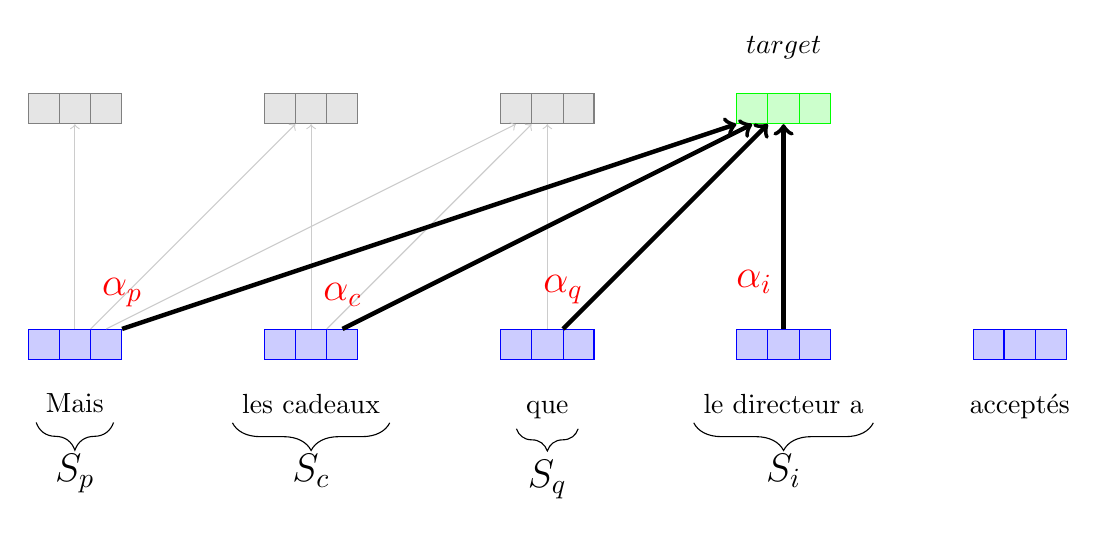
\begin{tikzpicture}[
      neurons/.style 2 args={
        rectangle split,
        rectangle split horizontal,
        draw=#2,
        rectangle split parts=#1,
        fill=#2!20}]

    %\node[red] (a1) at (0,1.5) {$\alpha_1$};
 \node[neurons={3}{gray}] (s1) at (0,3) {};
 \node[neurons={3}{gray}] (s2) at (3,3) {};
 \node[neurons={3}{gray}] (s3) at (6,3) {};
 \node[neurons={3}{green}] (s4) at (9,3) {};


\node (o1) [above=5mm of s4.center] {$target$};

 \node[neurons={3}{blue}] (x1) at (0,0) {};
 \node[neurons={3}{blue}] (x2) at (3,0) {};
 \node[neurons={3}{blue}] (x3) at (6,0) {};
 \node[neurons={3}{blue}] (x4) at (9,0) {};
 \node[neurons={3}{blue}] (x5) at (12,0) {};


\draw [->, color=gray!40] (x1) -- (s1);


\draw [->,color=gray!40] (x1) -- (s2);
\draw [->,color=gray!40] (x2) -- (s2);


\draw [->,color=gray!40] (x1) -- (s3);
\draw [->,color=gray!40] (x2) -- (s3);
\draw [->,color=gray!40] (x3) -- (s3);

\draw [->,ultra thick] (x1) -- (s4)node[pos=0,above,yshift=4pt,color=red] {\Large $\alpha_p$};
\draw [->,ultra thick] (x2) -- (s4)node[pos=0,above,yshift=4pt,color=red] {\Large $\alpha_c$};
\draw [->,ultra thick] (x3) -- (s4)node[pos=0,above,yshift=5pt,color=red] {\Large $\alpha_q$};
\draw [->,ultra thick] (x4) -- (s4)node[pos=0,left,yshift=17pt,color=red] {\Large $\alpha_i$};


\node (w1) [below=5mm of x1.center] {Mais};
 \node (w2) [below=5mm of x2.center] {les cadeaux};
 \node (w3) [below=6mm of x3.center] {que};
 \node (w4) [below=5mm of x4.center] {le directeur a};
 \node (w5) [below=5mm of x5.center] {acceptés};

 \draw[decorate,decoration={brace,amplitude=10pt,mirror}]
  (w1.south west) -- node[below=0.8em,font=\Large] {\textbf{$S_p$}} (w1.south east);
 
 \draw[decorate,decoration={brace,amplitude=10pt,mirror}]
  (w2.south west) -- node[below=0.8em,font=\Large] {\textbf{$S_c$}} (w2.south east);

  \draw[decorate,decoration={brace,amplitude=8pt,mirror}]
  (w3.south west) -- node[below=0.8em,font=\Large] {$S_q$} (w3.south east);

  \draw[decorate,decoration={brace,amplitude=10pt,mirror}]
  (w4.south west) -- node[below=0.8em,font=\Large] {$S_i$} (w4.south east);
\end{tikzpicture}
} \caption{Target representation as a linear combination of all preceding token representations, weighted by their attention scores $A^l_t =<\alpha_p, \alpha_c, \alpha_q, \alpha_i>$ }\label{fig:cqi_illustration}
\end{figure}

Given a sentence prefix $S=<S_p,S_c,S_q,S_i>$ for NA tasks, we aggregate groups of tokens into the following abstract variables (as illustrated in Figure~\ref{fig:cqi_illustration}): 

\begin{itemize}[topsep=0pt, partopsep=0pt,itemsep=0pt,parsep=0pt]
    \item $S_c$: \cue and its dependent words
    \item $S_q$: relative pronoun ``que''
    \item $S_i$: intermediate tokens between the \cue and \target, excluding those in $S_c$ and $S_q$
    \item $S_p$: tokens preceding $S_c$
\end{itemize}
The corresponding aggregated contextualized representations and attention weights are denoted as $R=\ <r_p,r_c,r_q,r_i>$ and $A^l=\ <\alpha_p, \alpha_c, \alpha_q, \alpha_i>$, respectively. The target representation, $r_t$, is obtained as the output of a pre-trained Transformer LM when given the sentence prefix $S$ as input: $r_t = \texttt{Transformer}(S)$. The causal model's outcome, denoted as $\mathcal{A} \in \{0,1\}$, indicates if the Transformer's predicted agreement feature matches the gold label, and is defined as the output of our NA tasks $\mathcal{A} = \texttt{NA}(r_t)$.


\paragraph{Causal assumptions} We make the following causal assumptions and formulate two types of hypotheses related to the most relevant tokens that influence the Transformer's agreement predictions. It is important to note that these hypotheses are not mutually exclusive.  
\begin{itemize}
    \item $r_t$ is causally dependent on $A^l$. The contextualized representation for the \target is computed, in a simplified view, as a linear combination of all the preceding token representations, $R$, weighted by the attention scores $A^l_t$.
    \begin{itemize}
        \item[-]  \textbf{Linear combination hypothesis:}  \textit{$r_c,r_q,r_i$ contribute similarly to $r_t$ and thus affect the model's prediction for S-V and O-PP agreement in a similar way.}\footnote{We exclude $S_p$ from our analysis in this study, as the low probing accuracy in probing experiments (\S\ref{sec:probing_location}) suggests that the agreement information is not encoded (in a useful way) in $r_p$. } \\
        Our probing experiments in Section~\ref{sec:probing_location} reveal very similar distribution patterns of agreement information across S-V and O-PP agreement: it is mainly encoded across tokens between the \cue and the \target.  
    \item[-] \textbf{Linguistic motivated hypothesis:} \textit{The tokens involved in the respective agreement rules serve as the main source of the agreement feature encoded in $r_t$.} \\ 
    Therefore, for the S-V agreement, $S_c$ is predominantly responsible for providing the agreement feature. In the case of the O-PP agreement, both $S_c$ and $S_q$ play important roles.
    \end{itemize}
    \item $\mathcal{A}$ is causally dependent on $r_t$, as agreement feature predictions are obtained by applying NA task through $r_t$.
\end{itemize}


In causal inference theory, the do(•) operator denotes an intervention on a causal diagram. In this study, we intervene on the attention weights between the \target and $S_c,S_q,S_i$ --- tokens that encode linearly extractable agreement information, and some of which are relevant to agreement rules. Concretely, the example in Figure~\ref{fig:mask_que} illustrates a do($\alpha_q = 0$) operation, which means intervening on the causal graph by setting $A^l_{t,q}$ --- the attention to ``que'' --- to be zero without changing any other variables. As the relative pronoun ``que'' plays a very different role in S-V agreement and O-PP agreement according to theoretic linguistics, we would expect different intervention effects resulting from do($\alpha_q = 0$) for the two types of agreement if the Transformer bases its predictions mainly on tokens involved in relevant agreement rules. Following the linguistic motivated hypothesis, we also expect that do($\alpha_c = 0$), which remove the direct contribution of the \cue, would result in a substantial degradation in the model's agreement prediction for both NA tasks. 

  

 \paragraph{Causal effect} We define the causal effect of a variable $\alpha_i$ on $\mathcal{A}=\texttt{NA}(r_t)$ as the difference in $\mathcal{A}$ between the original scenario (with original masked attention weights) and a counterfactual scenario (with the weight of $\alpha_i$ set to zero). Formally, for a specific sentence-variable pair ($S$,$\alpha_i$), the individual causal effect of $\alpha_i$ on $\mathcal{A}$ is:

\begin{align}
\Delta(S,\alpha_i) & = \texttt{NA}(r_t) - \texttt{NA}(r_t^\prime) \nonumber, \text{\ where} \\
r_t & = \texttt{Transformer}(S,A^{l}) \nonumber \\
r_t^\prime & = \texttt{Transformer}(S,A^{l}, \text{ do}(\alpha_i=0))
\label{eq:indiv_causal_effect}
\end{align}
The $\texttt{NA}(r_t)$ function implements our number agreement tasks, inputting target form representations and outputting agreement feature $\mathcal{A}$. The Transformer model, $\texttt{Transformer}(S,A^{l})$ function, processes the sentence prefix and yields $r_t$. Here, the causal effect of a token $i$ (whose attention weight to \target is $\alpha_i$) on $\mathcal{A}$ can be measured by $\Delta(S,\alpha_i)$. For instance, in Table~\ref{ex:mask_que}, for the original sentence prefix, the model predicts the correct agreement feature ($\texttt{NA}(r_t)=1$). After the intervention of forcing the attention weight between `que' and the \target to be zero, the model's prediction does not match the gold label, thus $\texttt{NA}(r_t^\prime)=0$. The causal effect of the token `que' on model's prediction $\mathcal{A}$ for this sentence is $\Delta(S,\alpha_q)$= 1.

\subsection{Causal experiments and results} \label{sec:causal_expe_res}
\paragraph{Experimental setup} Our experiments are based on the same NA tasks discussed in Section~\ref{sec:heuristics}. In this study, the evaluation sets for both types of agreement only include sentences for which the Transformer LM correctly predicted the agreement feature, based on the results described in Section~\ref{sec:h_eval_protocol}. More specifically, for S-V agreement, we have a dataset denoted as $\mathcal{D}^{\prime}_{s-v}=\{S^{(i)},\mathcal{A}^{(i)}\}$, where $i=$27,278, covering 98.9\% of the total examples in the entire S-V agreement evaluation set. Similarly, for O-PP agreement, we have $\mathcal{D}^{\prime}_{o-pp}=\{S^{(i)},\mathcal{A}^{(i)}\}$, with $i=$64,798, representing 94.6\% of the total examples from the entire O-PP agreement evaluation set (\S\ref{sec:NA_data}). Here, $(S^{(i)},\mathcal{A}^{(i)})$ stands for the pairing of a sentence prefix with the grammatical number of the \cue. Given the causal model in Figure~\ref{fig:causal_dag} and the equation of individual causal effect (\ref{eq:indiv_causal_effect}), before any intervention, the outcome $\mathcal{A}=\texttt{NA}(r_t)$ is consistently $1$ across both evaluation sets.

We then execute the NA tasks with the Transformer LM again (Section~\ref{sec:heuristics}), but with a twist: when predicting the target verb (only at this moment!), we apply causal interventions. These involve eliminating the direct attention from the \target to:
\begin{enumerate}[label=\roman*)]
    \item \( \mathcal{S}_{c} \), which includes the cue and its dependents;
    \item \( \mathcal{S}_{q} \), representing the relative pronoun \textit{que} in the \emph{context};
    \item both \( \mathcal{S}_{c} \) and \( \mathcal{S}_{q} \);
    \item \( \mathcal{S}_{i} \), which consists of all tokens in the \emph{context} excluding \( \mathcal{S}_{c} \) and \( \mathcal{S}_{q} \).
\end{enumerate}


\paragraph{Average causal effect} 
Considering the individual causal effect equation (\ref{eq:indiv_causal_effect}) and an evaluation set $\mathcal{D}$ (for which the probed model achieved 100\% accuracy before any interventions), we define the \ac{ACE} of a specific intervention $\alpha_i$ as:

\begin{equation}
ACE = \frac{\sum_{(S,\mathcal{A}) \in \mathcal{D}} \Delta(S,\alpha_i)}{|\mathcal{D}|}
\end{equation}

Simply put, ACE denotes the proportion of initially correctly predicted examples that are incorrectly labeled after an intervention $\text(do)(\alpha_i=0)$. $ACE$ can also be interpreted here as the performance degradation caused by a particular intervention.

 \begin{figure}[htbp]
\scalebox{.95}{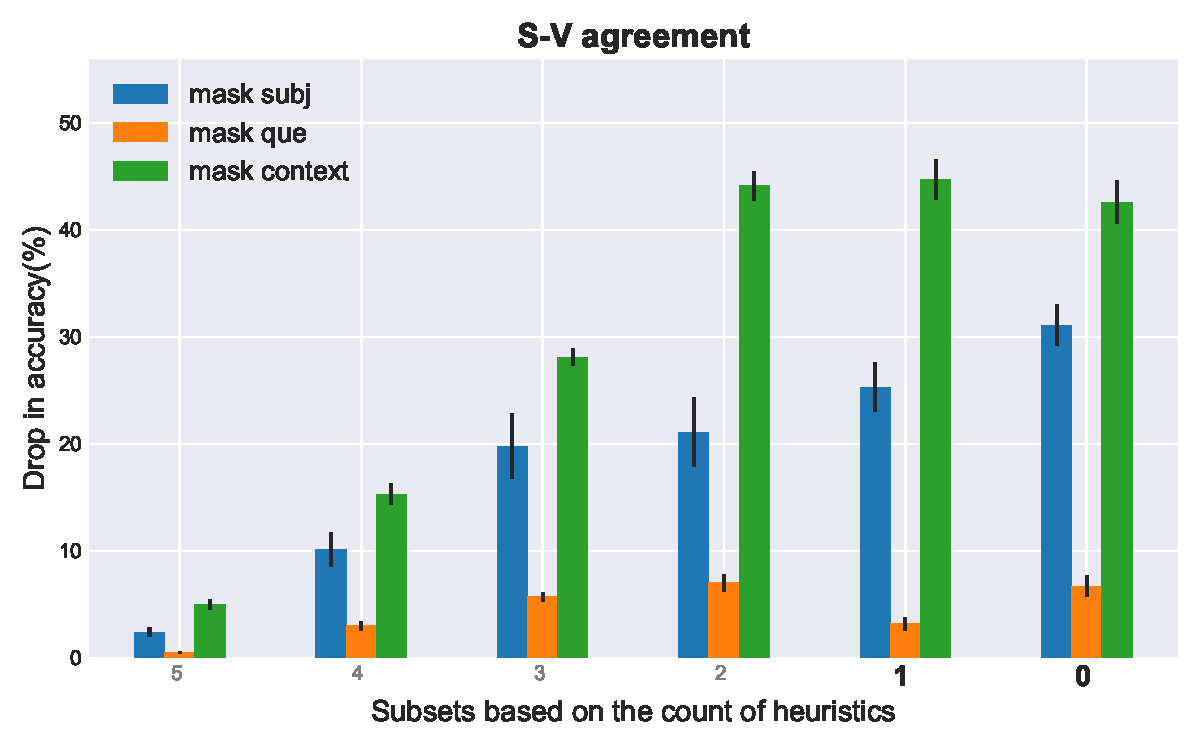
\includegraphics[width=\columnwidth]{figures/causal-subj-v.pdf}}
\scalebox{.95}{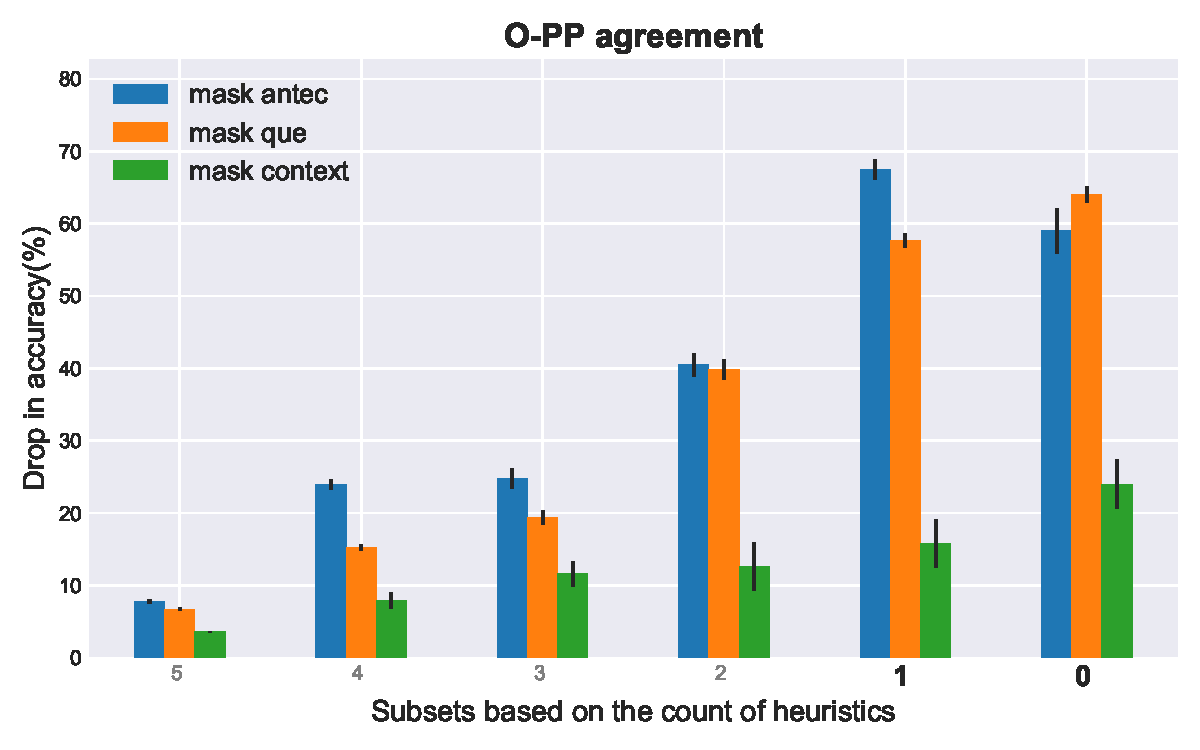
\includegraphics[width=\columnwidth]{figures/causal-obj-pp.pdf}}
\caption{Average causal effect of interventions on Transformer's NA task performance, quantified by drop in accuracy before and after different interventions, and further broken down based on prediction difficulty measured by the number of heuristics. The term \emph{cue} here refers to the antecedent and its modifiers (determiners and adjectives) in O-PP agreement, and to the subject and its modifiers in S-V agreement.} \label{fig:causal_res}
\end{figure} 

\paragraph{Results} In Figure~\ref{fig:causal_res}, we report the changes caused by different interventions, as quantified by the average causal effect. This effect represents the drop in performance on NA tasks for both S-V and
O-PP agreement.\footnote{See the Table~\ref{tab:full_causal_res} in the Appendix for the full results.} These causal effects are further dissected based on task difficulty. As noted in Section~\ref{sec:h_eval_protocol}, our investigation primarily focuses on the more challenging cases (i.e.\ \emph{0}
and \emph{1 heuristic} subsets), which cannot be resolved via surface heuristics and thus provide robust evidence of a model's capacity to capture sentence structure information.


As observed, the
\emph{cue} (i.e.\ the antecedent or subject groups) turns out to be critical
for predicting the corresponding agreement for both types of agreement. Masking these tokens
strongly degrades Transformer's performance on the 0-, 1-heuristic subsets. For the O-PP agreement, we notice a performance drop of over 59\%, and for the S-V agreement, a decline of over 25\%. Interestingly, the impact of other interventions on the two types of agreement displays marked differences. The role of the relative pronoun ``que'' in determining the form of the target verbs in these two agreement phenomena significantly diverges. In the case of O-PP agreement, masking the relative pronoun leads to a significant decrease in prediction accuracy, decreasing by over 57\%. Conversely, it has minimal effect on the prediction of subject-verb agreement, with accuracy decreasing by no more than 7 percentage points. This suggests that that even though the two agreement phenomena exhibit highly similar surface forms and the model encodes agreement information in a similar manner (as detailed in Section~\ref{sec:probing}), the Transformer uses separate agreement mechanisms to handle the S-V and O-PP agreements. This distinction thereby lends support to the linguistically-motivated hypothesis.


Figure~\ref{fig:causal_res} also demonstrates that, for S-V agreement across object relatives, the \emph{context} tokens excluding the \cue and ``que'', contribute more significantly to the model's decision than the subject group tokens (i.e., the subject and its dependents) with which the verb agrees. This indicates that \target receives more agreement information from intermediate tokens than from the direct attention to the nominal subject and its dependent words. This pattern contrasts with the O-PP agreement, where direct attention to the two linguistically-motivated components (i.e., antecedent and ``que'') can induce an over 80\% performance drop, compared to a maximum causal effect of 24\% for context tokens. This surprising observation appears to confirm the findings of \cite{ravfogel-etal-2021-counterfactual}, who suggested that to predict S-V agreement, the model uses information about relative clause boundaries encoded in its representations. To account for this intriguing observation, we hypothesize that while the agreement information is distributed across all tokens in the \emph{context} segment, the relative clause boundary information is vital for the model to determine how to use this information to inflect the main verb. This would clarify why the \emph{context} tokens play such a crucial role in controlling the agreement. However, further experiments are necessary to confirm this hypothesis.
 
\subsection{Conclusion} \label{sec:causal_discussion}
In this section, our objective is to identify which tokens mainly provide the agreement information used by the model to resolve the NA tasks, and further determine whether the usage pattern reflects the distinct theoretical modeling of S-V and O-PP agreement phenomena. To this end, we designed a causal experiment based on self-attention interventions. In this framework, the model performed the NA tasks from Section~\ref{sec:heuristics}, but with a twist: when predicting the \target, we cut the direct attention from the \target to tokens proposed to provide agreement information, based on two hypotheses: the linguistically motivated hypothesis and the linear combination hypothesis (supported by probing results in Section~\ref{sec:probing_location}). The model's post-intervention performance was then compared with the pre-intervention performance, with the performance drop indicative of the causal effect of the intervened tokens.


Our experimental findings reveal a distinct pattern in how Transformers use encoded agreement information across the S-V and O-PP agreements. In the case of O-PP agreement, both the \cue and relative pronoun ``que'' serve as crucial sources of agreement information. In contrast, for S-V agreement across relative clauses, while the \cue 
plays an important role in determining the \target's number, the relative pronoun ``que'' has minimal impact on the model's agreement behavior. This discrepancy aligns with the linguistically motivated hypothesis and resonates with the theoretical linguistic analysis of the two agreement phenomena, supporting the Transformer's representational adequacy for capturing syntactic information. Additionally, this reinforces the findings of~\cite{elazar2021amnesic, hanna-etal-2023-functional}, suggesting that the encoding of linguistic properties, as revealed by probing classifiers, may not necessarily be functionally relevant to the model's predictions. This highlights the importance of transitioning from correlational analysis to causal approaches for a more accurate understanding of model behavior. 

This study also opens up several avenues for future research. A primary focus could be on identifying token positions that provide misleading agreement information, leading to incorrect model behavior. To address this, a more controlled experimental setup is needed: Common error patterns from the model's predictions can be extracted (\S\ref{app:NA_error_pattern}), serving as the basis for creating a template-based evaluation set. Subsequently, the causal framework presented in this section could be applied to individual token positions to identify the sources of the model's erroneous predictions. Additionally, questions persist about the underlying mechanisms that allow the \textit{target} token to obtain precise agreement information from intermediate tokens, as well as how the model encodes and uses information about relative boundaries. These questions present compelling areas for future investigation.


\section{Word order: the impact of positional encoding on NLM's syntactic abstraction capacity } \label{sec:word_order_NA}

In the preceding section, we explored the inner workings of the Transformer language model by applying causal intervention on its self-attention mechanism. Our results indicate that the model is capable of leveraging the hierarchical structure of sentences for nuanced, grammar-based generalization. Yet, one might wonder how a Transformer-based language model can approximate a hierarchical understanding of sentence structure when it processes all tokens simultaneously from linear sequence input. To address this, the current section shifts focus to a critical aspect of language that the self-attention mechanism is not inherently equipped to handle: word order information.


Unlike RNNs, which naturally encode word-order information by sequentially processing input elements, the Transformer model processes all tokens in a sequence simultaneously. As a result, the Transformer does not inherently account for the order of the tokens. This order is crucial for many languages where position encodes grammatical functions. Even in free-order languages, token order remains significant, especially given tokenization into sub-word units, making it essential for tasks like language modeling. 

To address this, the Transformer integrates positional embeddings with token embeddings before feeding them into the self-attention mechanism. As detailed in Section~\ref{sec:auto_transformer}, autoregressive language models use an incrementally applied masked self-attention mechanism, which forces the model to attend only to preceding words. This could make positional embeddings redundant, as observed in recent work~\cite{haviv-etal-2022-transformer}. In contrast, masked language models do not have this inherent order modeling, making positional embeddings the sole source of order information.

This study aims to investigate the role of positional embeddings in language modeling and their impact on the syntactic abstraction capacity of Transformer-based language models. Building on the methodology of ablation studies~\citep{meyes2019ablation}, we perform a targeted ablation experiment that focuses on positional embeddings. We compare the performance of autoregressive Transformer LM with and without positional embeddings, and then we run similar experiments with bidirectional Transformer LM~\citep{devlin-etal-2019-bert}. Our experiment is designed to understand the relationship between the model's ability to abstract syntactic structures and its awareness of token order within a sequence.

\subsection{Positional embeddings in Autoregressive Transformer LM} \label{sec:exp_1_tm_nopos}

\paragraph{Experimental setup} In all our previous experiments, we considered an autoregressive Transformer LM, denoted as $\mathcal{M}$, with the sinusoidal positional embeddings described in \cite{NIPS2017_3f5ee243}, which is the standard setting. To delve deeper into the role of explicit position encoding within Transformer LMs, we consider a variant of this model without positional embeddings, denoted as $\mathcal{M}_{nopos}$. The training process for this position-deprived Transformer LM mirrors that of the original model, using the same training data and the same hyperparameters (\S\ref{app:tm_training}).

To assess the importance of positional embeddings for the language modeling objective itself, we conducted an intrinsic evaluation by comparing the validation set perplexity of the model $\mathcal{M}_{nopos}$ and the original model $\mathcal{M}$. As suggested by~\cite{hu-etal-2020-systematic}, perplexity scores do not always give us a clear picture of a model's syntactic ability. Therefore, we also conduct an extrinsic evaluation by comparing the performance of both models, $\mathcal{M}_{nopos}$ and $\mathcal{M}$, on NA tasks. This evaluation helps us assess the importance of explicit position encoding in the model's syntactic abstraction capacity.

 % for the language modeling objective
\paragraph{Results}  In terms of the perplexity obtained on the validation set, the model without positional embeddings, $\mathcal{M}_{nopos}$, has an average score of 27.2 across five pre-trained instances, which is strikingly close to the score of 27.0 for the original Transformer. This counterintuitive result suggests that explicit positional encoding may not be as crucial as we thought for pre-training the autoregressive Transformer LM. 

When it comes to accuracy on NA tasks, as shown in Figure~\ref{fig:tm_nopos_NA_tasks}, the ablation of positional embeddings surprisingly has a negligible impact. This holds true for both the overall accuracy and the stratified accuracies across subsets of varying difficulty, as determined by our heuristic-based evaluation protocol. Again, this is particularly striking considering the often crucial role of word order in encoding syntactic relationships in languages like French.

A plausible explanation for these surprising results is that the autoregressive Transformer's incremental attention mask, which forces each token to attend only to its preceding tokens, may inherently encode word order information. Although all tokens in a sequence are processed simultaneously, the ability of the model to take into account the predecessors of a given token may effectively allow it to deduce its position within the sequence. We explore this hypothesis in the following experiment. 



\begin{figure}[ht]
    \centering
    \begin{subfigure}[b]{0.49\textwidth}
        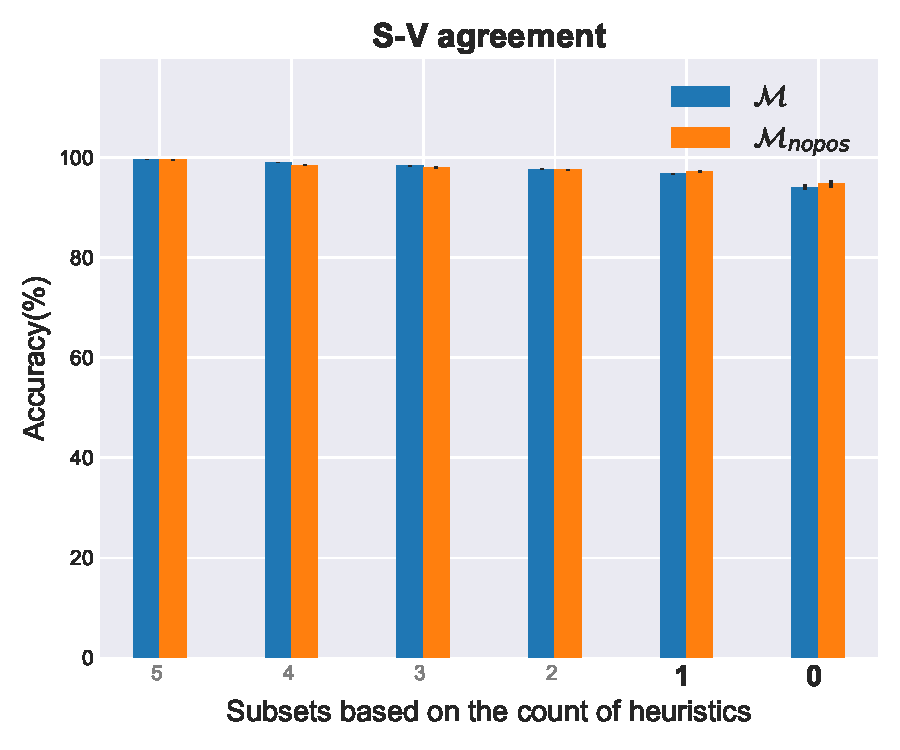
\includegraphics[width=\textwidth]{figures/tm-nopos-subj-v.pdf}
    \end{subfigure}
    \hfill
    \begin{subfigure}[b]{0.49\textwidth}
        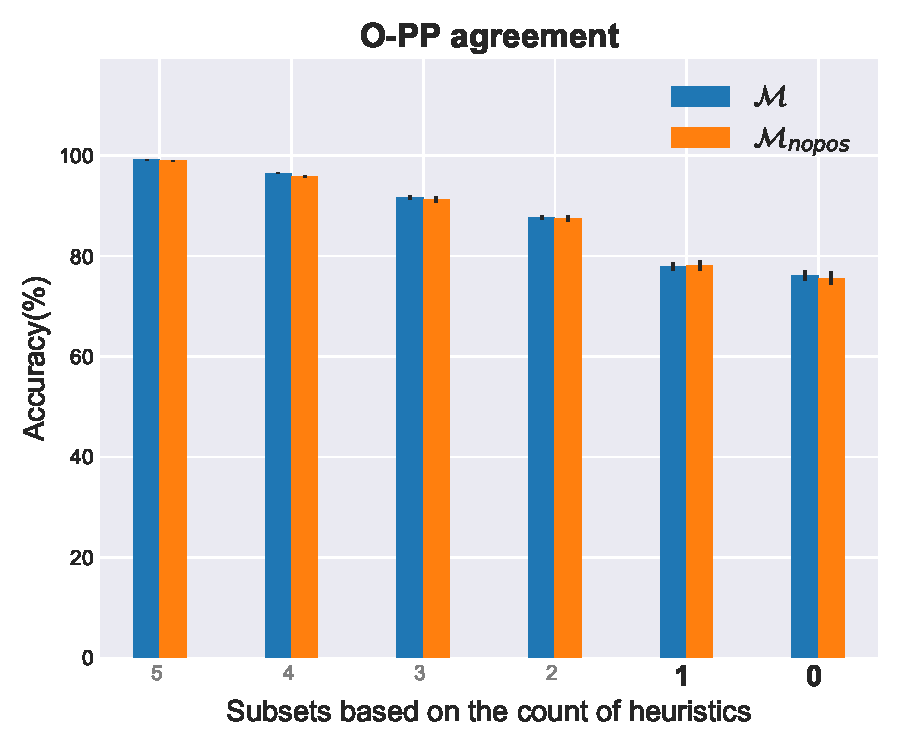
\includegraphics[width=\textwidth]{figures/tm-nopos-o-pp.pdf}
    \end{subfigure}
    \caption{Accuracy comparison of autoregressive Transformer LM on two NA tasks with and without positional embeddings. Detailed scores are reported in Appendix Table~\ref{tab:TM_nopos}. \label{fig:tm_nopos_NA_tasks}}
\end{figure}

 
\subsection{Positional embeddings in masked Transformer LM } \label{sec:exp_2_mlm_nopos}

The previous experiment reveals that an autoregressive Transformer LM deprived of positional embeddings can still perform comparably in language modeling and NA tasks. This leads us to hypothesize that the incremental self-attention mask might be enabling the model to implicitly reconstruct word order position information during the pretraining. To test this hypothesis, we extend our ablation experiment to a Transformer language model trained with a masked language modeling objective \citep{devlin-etal-2019-bert}. Unlike autoregressive language modeling, where the model predicts each subsequent word based on previous tokens, masked language modeling entails predicting randomly masked tokens using both preceding and succeeding context~(\S\ref{sec:lm_tasks}). In this context, positional embeddings serve as the sole source of order information. When removed, the MLM
generates token representations independent of the actual position of tokens in the input sequence, behaving like a bag-of-words model.  The goal here is to investigate whether MLMs can also implicitly learn word order during pre-training without explicit positional embeddings. If they cannot, it would suggest that the incremental attention mask indeed plays a crucial role in the autoregressive model's ability to learn word order information.


\paragraph{Experimental setup} We adapted our generic language model to implement a bidirectional Transformer model, which was then trained using a masked language modeling objective \citep{devlin-etal-2019-bert}. We pre-trained the MLMs both with and without positional embeddings on the same training data (as described in \ref{sec:heuristic_exp_setup}), following the same training process used for the autoregressive models. For each model, we train five different seeds using the optimal hyperparameter configuration.\footnote{Please refer to \S\ref{app:tm_training} for details on the hyperparameters.} We repeat the ablation experiment from \S\ref{sec:exp_1_tm_nopos} to compare the perplexity scores of the pretrained MLMs and their performance on NA tasks in the absence of positional embeddings.

As discussed in Section~\ref{sec:lm_tasks}, perplexity is a standard metric for evaluating autoregressive LMs. This metric is not suitable for models trained using a masked language modeling objective, where a masked token $w_i$ is predicted based on its surrounding context $S_{ \setminus i}$. To evaluate MLMs, we adopt the pseudo-perplexity approach from \cite{salazar-etal-2020-masked}, calculated as the average of the conditional log probabilities $log \mathbb{P}_{MLM}(w_i | S_{ \setminus i})$ for each token. While not comparable to conventional perplexity, it allows for a direct comparison between MLMs. More details can be found in the appendix~\ref{sec:ppl_lm}. 

\begin{figure}[ht]
    \centering
    \begin{subfigure}[b]{0.49\textwidth}
        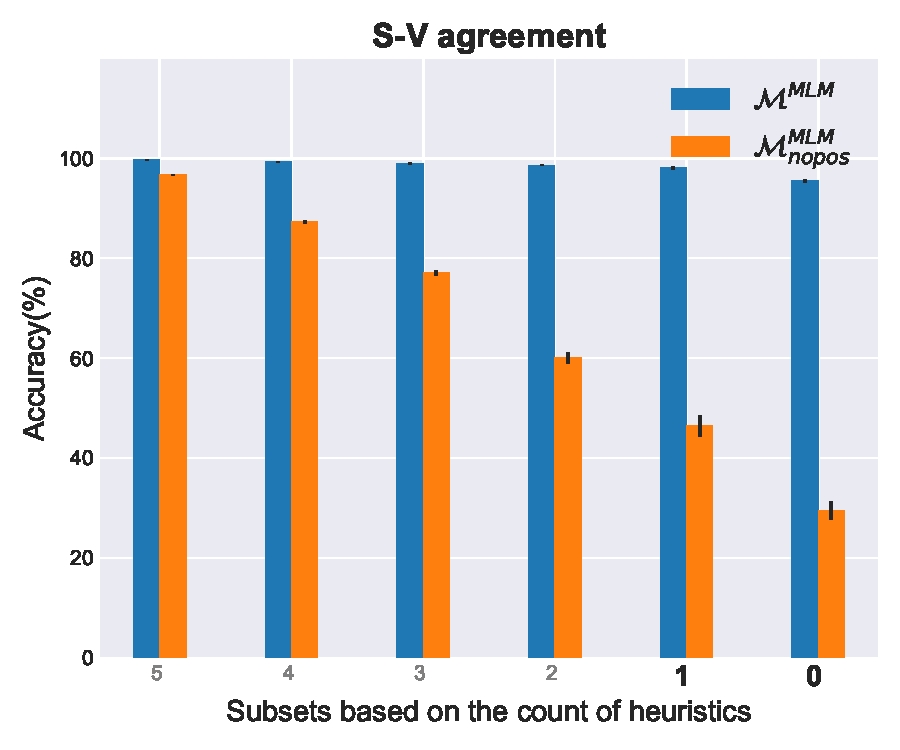
\includegraphics[width=\textwidth]{figures/mlm-nopos-subj-v.pdf}
    \end{subfigure}
    \hfill
    \begin{subfigure}[b]{0.49\textwidth}
        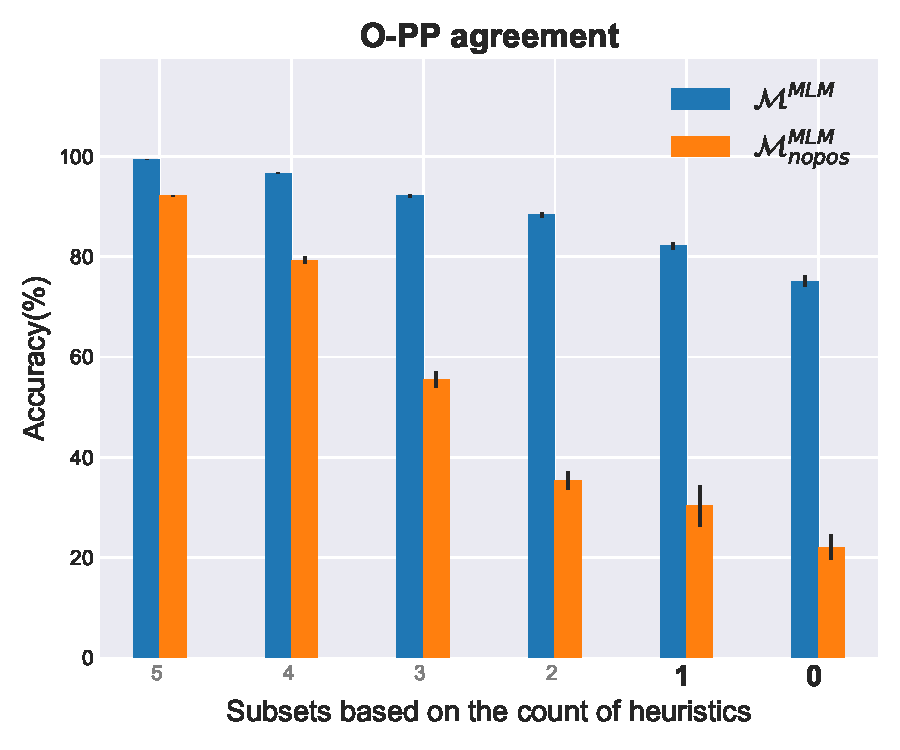
\includegraphics[width=\textwidth]{figures/mlm-nopos-o-pp.pdf}
    \end{subfigure}
    \caption{Masked Transformer LM's accuracy on two NA tasks with and without positional embeddings. Detailed scores are reported in Appendix Table~\ref{tab:MLM_nopos} \label{fig:mlm_nopos_NA_tasks}}
\end{figure}

\paragraph{Results}
Our experiments show a substantial difference in pseudo-perplexity scores between the masked language models with and without positional embeddings. The position-aware MLM converges to a very low score of 5.6, whereas the \texttt{nopos} MLM performs significantly worse, with a score of 57.2. This result aligns with the observations of previous studies such as \cite{sinha-etal-2021-masked} and \cite{haviv-etal-2022-transformer}, which noted that MLMs deprived of explicit position encoding suffer a substantial decline in pretraining task performance.

Regarding the performance on number agreement tasks, as seen in Figure~\ref{fig:mlm_nopos_NA_tasks}, the ablation of positional embeddings leads to a substantial decrease in accuracy across both agreement tasks. Particularly, in the most challenging cases, the performance drop reaches 66\% for S-V agreement and 53\% for O-PP agreement. These findings indicate that explicit position encoding plays a critical role in MLM's syntactic abstraction ability. This, in turn, provides evidence supporting our initial hypothesis concerning autoregressive LM, suggesting that the incremental attention mask may enable it to implicitly reconstruct absolute word position information.



\subsection{Conclusion}
In this study, we have performed a set of positional embedding ablation experiments with both autoregressive and bidirectional Transformer LMs. These models are evaluated based on their performance in language modeling and number agreement tasks, comparing the outcomes of models with positional embeddings against those without. Our results show that the autoregressive language model deprived of positional embeddings (\texttt{nopos}) achieves competitive performance compared to its original counterpart in both the language modeling task and the NA tasks. In contrast, bidirectional language models without positional embeddings experience substantial performance degradation in both language modeling and NA tasks. This stark contrast highlights the critical role positional embeddings play in bidirectional models in identifying token positions. Meanwhile, autoregressive LMs appear to leverage the incremental attention mask to implicitly reconstruct word order information, thereby the absence of explicit position encoding has very little impact on the model's performance.

\section{Conclusion and discussion} \label{sec:conclu_main_projct}
In this chapter, we conducted a contrastive study to explore the core question of my thesis: Does the Transformer language model exploit abstract sentence structures, or does it primarily rely on surface patterns when handling structure-sensitive phenomena? Our primary goals are twofold: to assess the behavioral and representational adequacy of the autoregressive Transformer model in relation to human syntactic processing, and to develop a linguistically-informed framework to enhance the interpretability of this complex model. To achieve this, we use number agreement tasks to explore how the Transformer LM processes two forms of agreement in French: long-distance subject-verb and object-past participle agreements, both involving object relative clauses. While these two types of agreement share superficial similarities in word sequences, their linguistic analyses fundamentally diverge.

Our approach begins with the proposal of a heuristic-based evaluation protocol, which effectively constrains the impact of surface heuristics in conventional number agreement tasks, providing a robust groundwork for our subsequent experiments. In our initial set of experiments, we assessed the ability of an autoregressive Transformer language model to predict these two types of agreement. The results indicate that the model exhibits high predictive accuracy, even under challenging conditions where all surface heuristics fall short. Further control experiments underscore the Transformer's ability to generalize beyond collocational cues and strong frequency biases. Taken together, these results strongly suggest that the Transformer is not merely exploiting surface patterns, but may be capturing some form of abstract sentence structure. This evidence indicates that Transformer meets the first prerequisite --- behavioral-level similarity --- for genuine syntactic generalization.


Building on the strong behavioral performance of the Transformer, we took a more in-depth investigation to assess where syntactic agreement information is located within the model's inner representations, as a measure of its representational adequacy. Our second set of experiments, using a probing approach, reveal that the relevant agreement information is mainly linearly encoded across all tokens between the \cue and the \target. Interestingly, within the contextualized representations, this information is found in a small number of highly correlated dimensions, while also being fuzzily encoded in a redundant manner across the remaining dimensions. Notably, we observe a very similar distribution pattern of agreement information for both types of agreement phenomenon.

To go beyond the limitations of probing, which mainly reveals correlations between encoded information and the model behavior, we introduced a causal framework. This framework relies on counterfactual analysis and involves intervening directly on the model's self-attention mechanism. Our causal experiments provide further evidence that the Transformer model's success is based on linguistically justified cues, consistent with French grammar. Importantly, the abstract structure uncovered by the Transformer model aligns with the distinct theoretical modeling of the two structure-sensitive phenomena we examined. This alignment supports the Transformer's representational adequacy for capturing syntactic information, suggesting that its internal mechanisms are not merely statistically efficient but also linguistically meaningful. Consequently, this lends additional credibility to the potential of the Transformer as an explanatory tool for human syntactic processing. 

 
Additionally, to investigate how Transformer language models approximate syntactic structures from string input, we conducted a set of positional embedding ablation experiments with autoregressive and bidirectional Transformer LMs. We find that explicit position encoding has little impact on the general function and syntactic abstraction ability of the autoregressive LM. This is likely because the model can leverage the absolute word order information from the incremental attention mask. 

Our study represents an initial step towards a deeper understanding of how neural language models function. Our analysis framework, which begins with behavioral syntactic tasks fortified by heuristic-based evaluation, then pairs with linguistic probes, and finally explores through counterfactual analysis via causal intervention, provides a robust methodology to assess the syntactic abstraction capacity of neural language models. Notably, our findings regarding the linguistically motivated distribution of syntactic information in Transformers' representations could extend easily to other linguistic phenomena and languages.

Nevertheless, many questions remain unresolved, such as the precise mechanism by which Transformers track agreement information and how they encode long-distance dependencies from linear word sequences. It is also of interest to explore whether the model can emulate a human-like rule-based generalization to dynamically recombine familiar structures in novel situations. These avenues represent exciting directions for further investigation. Our work thus far only marks the beginning of a rich and exciting journey toward deciphering the complex inner workings of neural language models.

\part{Assessing model capacity to generalize compositionally observed structures }
\chapter{SLOG: A Structural Generalization Test for Semantic Parsing} \label{chp:slog}


\startcontents[chapters]
\printmyminitoc{
}


\noindent In the previous part of this dissertation, we assessed the syntactic capabilities of an autoregressive Transformer, specifically focusing on its ability to handle two syntax-sensitive phenomena. Our findings indicate that the model acquires remarkably nuanced representations of sentence structure, as evidenced by its strong performance on both behavioral-level tasks and measures of representational adequacy when evaluated on unseen, held-out evaluation sets.  


However, this leads us to another critical dimension of inquiry: the nature and depth of the model's observed syntactic generalization. Early studies by \cite{fodor2002compositionality} and \cite{marcus2003algebraic}
posited that neural language models like RNNs may lack the capacity for genuine compositional syntactic generalization due to the absence of explicit symbolic representation. These models, they argued, often rely on similarity-based inference derived from patterns encountered during training. This notion is supported by recent studies, such as \cite{bender2021dangers}, which describe language models as ‘‘stochastic parrots’’ that primarily memorize and shallowly recombine observed examples. Additionally, the capacity for extensive memorization in neural models is well recognized in the literature~\citep{halevy2009unreasonable,zhang2021understanding}.

Let's consider the case of subject-verb agreement across relative clauses, as detailed in Section \ref{sec:two_agreements}. Our findings from Chapter~\ref{chp:main_project} suggest that the Transformer leverages the structural relationships between words to accurately predict the long-distance dependency illustrated in (\ref{ex:slog_s-v}).
\vspace{-0.25\baselineskip}
\begin{exe}
    \ex \label{ex:slog_s-v} \textsc{Target sentence:} \textcolor{orange}{\textbf{NP$_1$}} + \textcolor{blue}{Relative Clause$_1$} + \textcolor{orange}{\textbf{V$_1$}}
    \ex Compositional generalization:
    \begin{xlist}
        \ex \label{ex:S-V_local} \textcolor{orange}{\textbf{NP$_2$}} + \textcolor{orange}{\textbf{V}$_2$}
        \ex \label{ex:N-RC} ... V + \textbf{NP}$_3$ + \textcolor{blue}{Relative Clause$_3$}.
    \end{xlist}
    \ex \label{ex:slog_simi_s-v}Similarity-based generalization:  \textcolor{orange}{\textbf{NP$_4$}} + \textcolor{blue}{Relative Clause$_4$} + \textcolor{orange}{\textbf{V$_4$}}
\end{exe}
\vspace{-0.25\baselineskip}
As proposed by Fodor and Marcus, we can hypothesize two potential ways the model learns such a structural relationship. First, the model might rely on training sentences such as (\ref{ex:S-V_local}) and (\ref{ex:N-RC}). By compositionally combining these structures, the model could infer the long-distance dependency relationship in (\ref{ex:slog_s-v}). This approach exemplifies compositional generalization. Second, the model might extrapolate grammatical knowledge from training sentences like in (\ref{ex:slog_simi_s-v}) to the target sentence (\ref{ex:slog_s-v}) based on their structural similarity. In this process, the model could grasp concepts like syntactic subjecthood, morpho-syntactic number, and the boundaries of relative clauses, subsequently formulating distributional rules at these abstract category levels. By recapitulating its training data through structural similarity and lexico-categorical abstraction, the model can generalize to unfamiliar sentences with known structures. Given that in Chapter~\ref{chp:main_project} we do not control the types of syntactic structures in the model's pretraining data, it is plausible that the model's performance on unseen sentences is driven more by memorization of structures encountered in the training data than by genuine compositional generalization.


This brings us to the core questions: To what extent do these models rely on memorizing structures they have encountered during training? More importantly, can these models achieve generalizable abstractions by compositionally applying observed syntactic rules to interpret new, unseen linguistic patterns? While systematic compositional generalization is a key component in human linguistic cognition, it remains an open question whether these neural models can also dynamically recombine known elements in a compositionally consistent manner with their underlying syntactic structure.



To explore these questions, the current chapter introduces a compositional generalization challenge test. This test aims to directly probe the model's capability to compositionally interpret unseen syntactic constructions through the combination of known structures, and will include experiments with similar Transformer-based models.

\paragraph{Outline} In this chapter,\footnote{This chapter stems from my visiting project at New York University, mentored by Prof. Tal Linzen and Dr. Najoung Kim, and conducted in collaboration with Alexander Koller, Yuekun Yao, and Lucia Donatelli. This chapter draws largely from our paper titled ``SLOG: A Structural Generalization Benchmark for Semantic Parsing'', which I primarily authored and has been accepted by EMNLP 2023.} Section \ref{sec:slog_intro} outlines the foundational aspects of compositional generalization and the semantic parsing task, followed by an introduction to the COGS benchmark \citep{kim-linzen-2020-cogs}, which serves as the starting point of this study. Section \ref{sec:slog_dataset} provides an overview of our SLOG benchmark, a dataset specifically constructed to focus on compositional structural generalization. Section \ref{sec:data_generation} details the dataset generation, and Section \ref{sec:slog_ex_setup} describes the experimental setting, discussing the models evaluated and the evaluation metric. Moving on to Section \ref{sec:slog_res}, we present the findings of our investigation into three Transformers-based models and a structure-informed parsing model. And Section \ref{sec:slog_conclu} provides a summarizing conclusion. 

\section{Introduction} \label{sec:slog_intro}

The immense productivity of human language enables us to understand and produce a potentially infinite number of sentences from finite input elements \citep{chomsky1965aspects, hauser2002faculty}. This linguistic productivity is generally attributed to the principle of compositionality --- the assumption that the meaning of an expression is a function of the meanings of its components and the way they are syntactically combined \citep{frege_1892,partee1984compositionality}. Reflecting this principle, human linguistic competence exhibits \emph{compositional generalization}: the algebraic capacity to understand and produce novel sentences by reassembling known elements \citep{montague1974c}. 

Central to this compositional generalization are two key concepts: \textit{systematicity} and \textit{productivity}, as presented by~\cite{fodor1988connectionism}. Systematicity refers to the consistent application of compositional rules to linguistic elements to derive meaning. This is analogous to how algebraic functions are consistently applied to appropriate variables. In practical terms, systematicity allows humans to extend their understanding to sentences or concepts that are systematically related. Productivity, on the other hand, is the ability to generate an infinite variety of sentences or thoughts from a finite set of words or concepts. In language, this is seen in our ability to produce and understand new sentences that we have never encountered before. 

A classic illustration of this, presented by Fodor, is that people who know the meaning of \emph{John loves Mary}, along with its underlying syntactic rules, can naturally understand the meaning of \emph{Mary loves John}, despite never having encountered it before \citep{fodor1988connectionism}. This exemplifies the systematicity in human language, where understanding such sentences involves the application of the same rules to recombine the same lexical units. In these two sentences, the verb \textit{loves} operates as a function, taking two variables (the subject and the object) and recombining the lexical units \textit{John} and \textit{Mary} in a way that generates different semantic meanings. This rule-based systematic generalization mechanism is widely assumed as the means humans use to handle linguistic productivity. 


Recent advances in NLP, particularly those based on neural networks, do not explicitly rely on the principle of compositionality. Despite this, their empirical success in various tasks suggests that they must have some form of effective generalization. This raises the question: Do these models learn to generalize in a manner similar to human-like compositional understanding, capturing both systematicity and productivity?
In recent years, a growing body of research has explored whether models possess such capability. Benchmarks for compositional generalization in semantic parsing have emerged as a useful tool to assess model's compositional capability \citep{lake2018generalization,hupkes2020compositionality,keysersmeasuring,kim-linzen-2020-cogs}. Semantic parsing tasks in these studies involve translating natural language expressions into semantic representations. The models are evaluated on a \emph{generalization set}, which is sampled from a distribution that systematically differs from the training distribution. This shift from training to evaluation is designed under the principle of compositionality and often includes new combinations of lexical units and observed rules, deeper recursions of observed patterns, or longer sequences. 

\begin{figure}[H]
\vspace{-3mm}  % reduce space above the figure
\captionsetup[subfigure]{font=normalsize}
%\captionsetup{width=0.98\textwidth}
    \centering
    \scalebox{0.78}{
    \begin{subfigure}{0.9\textwidth}
        \centering
    \begin{forest}
        for tree={s sep=5mm,, inner sep=0, l=0,} 
        [,phantom,s sep=2.5cm
        [  S 
            [ NP [Emma]]
            [ VP
                [ V [saw ] ]
                [ NP ,alias=o, tikz={\node [draw, dashed, white,fill=orange!30, fill opacity=0.20, fit=()(!1)(!l)]{}; }
                     [the dog, roof]   
                ]
            ]
        ]
        [S , tikz={\node [draw, dashed,white,fill=blue!30, fill opacity=0.15, fit=()(!11)(!lll)]{};} 
            [NP, alias=w, 
                 [The cat, roof]      
            ]
            [VP, [V,alias=a,[ran, [,no edge] ]
                 ]    
            ]
        ]
        [S , tikz={\node [draw, dashed,white,fill=blue!20, fill opacity=0.15, fit=()(!11)(!lll)]{};} 
            [NP,  tikz={\node [draw, dashed,white,fill=orange!30, fill opacity=0.25, fit=()(!1)(!l)]{};}
                 [The dog, roof]      
            ]
            [VP,
                [V, alias=b, [ran, [,no edge] ]
                ]  
            ]
        ]
        ]
        \tikz[overlay] \node[] (plus) at ($(o)!.5!(w)$) {\scalebox{1.5}{+}};
        \tikz[overlay] \node[] at ($(w)!.5!(b)$) {\scalebox{1.5}{$\leadsto$}};
    \end{forest}
    \caption{Lexical generalization: object $\rightarrow$ subject (COGS) } \label{fig:cogs_lex_gen}
    \end{subfigure}}
    \scalebox{0.75}{
    \begin{subfigure}{0.9\textwidth}
        \centering
        \begin{forest}
        for tree={s sep=2mm,, inner sep=0, l=0}
        [,phantom,s sep=3cm
        [S 
            [NP [Emma]]
            [VP
                [V [saw ]]
                [NP, tikz={\node [fill=green!30, fill opacity=0.25, fit=()(!1)(!l)]{};} 
                    [NP,  [the dog, roof]]
                    [PP, 
                        [P [on]]
                        [NP, alias=a,tikz={\node [fill=green!30, fill opacity=0.25, fit=()(!1)(!l)]{};}
                            [NP,  [a mat, roof]]
                            [PP,  [in a box, roof]]
                        ]
                    ]
                ]
            ]
        ]
        [S 
            [NP [Emma]]
            [VP
                [V [saw ]]
                [NP, tikz={\node [fill=green!30, fill opacity=0.25, fit=()(!1)(!l)]{};} 
                    [NP, alias=b, [the dog, roof]]
                    [PP
                        [P, [on]]
                        [NP, tikz={\node [fill=green!30, fill opacity=0.25, fit=()(!1)(!l)]{};}
                            [NP,  [a mat, roof]]
                            [PP 
                                [P [in]]
                                [NP,tikz={\node [fill=green!30, fill opacity=0.25, fit=()(!1)(!l)]{};}
                                    [NP, [a box, roof]]
                                    [PP, [in a house, roof]]
                                ]
                            ]
                        ]
                    ]
                ]
            ]
        ]
        ]
    \tikz[overlay] \node[] at ($(a)!.5!(b)$) {\scalebox{1.5}{$\leadsto$}};
    \end{forest}
    \captionsetup{skip=2em} 
    \caption{Structural generalization: deeper recursion depths (COGS \& SLOG) } \label{fig:cogs_struc_gen}
    \end{subfigure}}
        \scalebox{0.75}{
    \begin{subfigure}{0.9\textwidth}
        \centering
    \begin{forest}
        for tree={s sep=3mm,, inner sep=1, l=0}
        [, phantom, s sep=2.5cm
        [,phantom,s sep=3.5cm
        [S 
            [NP [Emma]]
            [VP 
                [V [saw ] ]
                [NP , alias=o, tikz={\node [draw, dashed, white,fill=green!30, fill opacity=0.20, fit=()(!1)(!ll)]{};}
                    [NP  [the dog, roof]]
                    [RC ,alias=e, [that Max held \_, roof]   
                    ]
                ]
            ]
        ]
        [S , tikz={\node [draw, dashed,white,fill=blue!30, fill opacity=0.15, fit=()(!11)(!lll)]{};} ,alias=h,
            [NP , alias=w,
                 [The cat, roof]  
            ]
            [VP
                [V, [ran, [,no edge] ]
                ] 
            ]
        ]
        ]
        [, phantom, s sep=2.5cm
        [S, tikz={\node [draw, dashed,white,fill=blue!30, fill opacity=0.15, fit=()(!111)(!lll)]{};}
            [NP , tikz={\node [fill=green!30, fill opacity=0.25, fit=()(!11)(!ll)]{};}
                [NP, [The dog, roof]]
                [ RC,alias=b,   [that Max saw \_, roof]
                ]
            ]
            [VP
                 [V, [ran, [,no edge] ]
                ] 
            ]
        ]
        ]
        ]
        \tikz[overlay] \node[] (plus) at ($(o)!.6!(w)$) {\scalebox{1.5}{+}};
        \tikz[overlay] \node[] at ($(w)!.4!(b)$) {\scalebox{1.5}{$\leadsto$}};
    \end{forest} 
    \caption{Structural generalization: RC object $\rightarrow$ RC subject (SLOG) }  \label{fig:slog_struc_gen}
    \end{subfigure}}
    \caption{
    Examples of lexical generalization in COGS --- (a), and structural generalization in COGS --- (b) and in SLOG --- (b, c). The SLOG task requires mapping the generalization examples to their logical forms; the corresponding logical forms are shown in Table~\ref{tab:cogs-lf}. 
    }
    \label{fig:lex_struc_gen}
    \vspace{-3mm}
\end{figure}

The COGS (\textbf{CO}mpositional \textbf{G}eneralization
Challenge based on \textbf{S}emantic Interpretation) dataset \citep{kim-linzen-2020-cogs} in particular has become a widely used benchmark, as it is designed to expose a generalization gap between training and testing data that many recent semantic parsers still struggle with. COGS distinguishes two types of generalization challenges that require different types of algebraic compositional strategies: \textit{lexical generalization} tests the ability to interpret novel combinations of known lexical items and known linguistic structures (Figure~\ref{fig:cogs_lex_gen}), and \textit{structural generalization} tests the ability to combine known structures into a novel structure (Figure~\ref{fig:cogs_struc_gen} and~\ref{fig:slog_struc_gen}). Importantly, the majority of generalization types in COGS target lexical generalization (18 of 21 generalization types, 86\% of the dataset). As lexical generalization is arguably easier than structural generalization (e.g., solvable by simple slot-filling), this imbalance may lead to overall performance numbers that are overly optimistic with regard to a model's capacity to generalize compositionally, as pointed out by \cite{weissenhorn-etal-2022-compositional} and \cite{yao-koller-2022-structural}. 




To facilitate a more comprehensive evaluation of structural generalization, we introduce SLOG, a \textbf{S}tructural \textbf{LO}ng-distance dependencies \textbf{G}eneralization benchmark. SLOG extends COGS to include 17 cases of structural generalization in total (14 new cases and 3 existing cases from COGS) (\S\ref{sec:slog_dataset}). The novel generalizations we introduce target two key structural features of human language: recursion and filler-gap dependencies.

Prior research has extensively investigated the processing of recursive constructions, a key feature of human language enabling the creation of complex, nested structures and hierarchical relationships~\citep{hauser2002faculty}. This area of study spans both artificial neural networks and human cognition \citeti{christiansen1999toward,lakretz2021can,mccoy2021infinite}.
Using artificial languages to isolate syntactic properties, research has shown that humans can learn and extrapolate nested patterns to deeper levels \citep{mccoy2021infinite}. In contrast, the capabilities of Transformer-based models in capturing recursive regularities have yielded mixed results \citep{bhattamishra-etal-2020-ability,hahn:2020,ebrahimi-etal-2020-self,lakretz2021can}. For filler-gap dependencies, a particularly challenging type of long-distance dependency involves generalization about the absence of material. Prior work has centered on syntactic tasks involving \textit{wh}-questions or relative clauses \citeti{wilcox-etal-2018-rnn,marvin-linzen-2018-targeted,li-etal-2023-assessing}. These studies primarily use language modeling as the task and do not 
require mapping to semantic representations. SLOG diverges from these works by incorporating recursion and filler-gap dependency in a more naturalistic setting and directly assess the semantic mapping. Importantly, rather than isolating syntactic generalization from linguistic meaning, our approach aims to assess whether models rely on syntactic generalization that aligns with human inductive biases to derive the meaning of complex sentences.

We use SLOG to evaluate a Seq2Seq Transformer model trained from scratch \citep{NIPS2017_3f5ee243}, two pre-trained Transformers (T5-base; \citealt{2020t5} and LLaMA; \citealt{touvron2023llama}), and a structure-informed\footnote{In this study, `structure-informed' refers specifically to models that incorporate explicit representations of linguistic structure.} model (AM-Parser; \citealt{weissenhorn-etal-2022-compositional}). In comparison to their overall performance on COGS, all models exhibit considerably lower performance on SLOG (\S\ref{sec:slog_res}). The generalization accuracy of Transformer-based models, including pre-trained ones, only reaches 40.6\%, and even a structure-informed parser, while exhibiting near-perfect generalization on COGS structural cases, only achieves 70.8\% on SLOG. The cases in which models struggle exhibit distinct patterns and suggest varied approaches of models to solving the task. An error analysis reveals that the AM-Parser generalizes well on existing structural generalization cases in COGS but struggles with the gap constructions introduced in SLOG due to inherent structural limitations, which we discuss in Section~\S\ref{subsec:am_parser_analysis}. Transformers tend to erroneously repeat frequent meaning representation subsequences observed during training. Even with pretraining, they struggle with unseen long-distance dependencies, which we attribute to their bias towards shorter predicate-argument dependencies~(\S\ref{subsec:long_distance_hard}). 

Overall, the discrepancy in performance between SLOG and COGS illuminates the notable gap between models' lexical and structural generalization abilities. It highlights the utility of SLOG in exposing the limitations of current models that have been shown to achieve high performance on existing generalization benchmarks, and helps foreground the different weaknesses of these models. While Transformer-based models can approximate compositional behavior to a certain extent, our findings suggest that they do not seem to rely on the kind of syntactic generalization rooted in symbolic compositional rules, which are believed to drive human linguistic systematicity and productivity. 


\section{Overview of SLOG benchmark} \label{sec:slog_dataset}
SLOG follows the semantic parsing format used in COGS, where the task is to translate English expressions into logic-based meaning representations (Table~\ref{tab:cogs-lf}). The dataset structure follows the basic design principles of COGS: there is a systematic gap between the training set and the generalization set, where target constructions in the generalization set are not included in the training set, but pieces of the training set can be recombined to arrive at their correct meanings. For example, as illustrated in example (c) of Table~\ref{tab:cogs-lf}, noun phrases that appear only in object position during training must be reinterpreted in subject position during generalization. 







\begin{table*}[htb!]
    \small
    \centering
    \setlength{\tabcolsep}{3pt}
    \begin{tabularx}{\linewidth}{p{12mm}>{\raggedright\arraybackslash}X @{\hspace{0.7em}} >{\raggedright\arraybackslash}X}
    \toprule
        & \textbf{Training}  
        & \textbf{Generalization} \\ 
        \midrule
        COGS
         & (a)The cat \textbf{ran}. \newline $\leadsto$ \lform{*cat($x_1$); run.agent($x_2,x_1$)} \newline
         Emma saw \textbf{the dog}.  \newline
         $\leadsto$ \lform{*dog($x_3$);see.agent($x_1,$Emma) $\land$ see.theme($x_1, x_3$)} 
         &  \textbf{The dog} ran. \newline
        $\leadsto$ \lform{*dog($x_1$); run.agent($x_2,x_1$)} \\ 
         %\cmidrule(l){2-3}
         \midrule
        \makecell[tc]{COGS \\ \&\\ SLOG} & (b) Emma saw the dog \textbf{on a mat in a box}.  \newline
        $\leadsto$ \lform{*dog($x_3$);see.agent($x_1,$Emma) $\land$ see.theme($x_1, x_3$) dog.nmod.on($x_3,x_6$) $\land$ mat($x_6$) $\land$ mat.nmod.in($x_6,x_9$) $\land$ box($x_9$)} 
         &  Emma saw the dog \textbf{on a mat in a box in a house}. \newline
         $\leadsto$\lform{*dog($x_3$);see.agent($x_1,$Emma) $\land$ see.theme($x_1, x_3$) dog.nmod.on($x_3,x_6$) $\land$ mat($x_6$) $\land$ mat.nmod.in($x_6,x_9$) $\land$ box($x_9$) $\land$ box.nmod.in($x_9,x_{12}$) $\land$ house($x_{12}$)} \\ 
        \midrule
         SLOG 
         &(c) The cat \textbf{ran}. \newline $\leadsto$ \lform{*cat($x_1$); run.agent($x_2,x_1$)}\newline
         Emma saw \textbf{the dog that Max held}. \newline 
         $\leadsto$ \lform{*dog($x_3$); see.agent($x_1,$Emma) $\land$ see.theme($x_1, x_3$) $\land$ dog.nmod($x_3,x_6$) $\land$ hold.agent($x_6,$Max) $\land$ hold.theme($x_6,x_3$)} 
         
         &  \textbf{The dog that Max saw} ran. \newline
         $\leadsto$ \lform{*dog($x_1$); see.agent($x_4,$Max) $\land$ see.theme($x_4,x_1$) $\land$ dog.nmod($x_1,x_4$) $\land$ run.agent($x_5,x_1$)} \\ 
         \bottomrule
    \end{tabularx}
    \caption{
        Examples of two distinct types of generalization: lexical generalization in COGS --- (a), structural generalization in COGS---(b) and in SLOG --- (b, c). The symbol $\leadsto$ indicates the task of translating an English sentence into its corresponding meaning representation.
    }\label{tab:cogs-lf}
\end{table*}



SLOG is generated using manually specified rules (\S\ref{sec:data_generation}), adopting the same meaning representation as COGS. The COGS \ac{LF}, derived from \cite{reddy-etal-2017-universal}, is based on Neo-Davidsonian view of verbal arguments. In this approach, the semantic units are mapped to indexed variables. For example, in: 
\vspace{-0.5\baselineskip}
\begin{exe}
    \ex The cat \textbf{ran}. \newline $\leadsto$ \lform{*cat($x_1$); run.agent($x_2,x_1$)} 
\end{exe}
\vspace{-0.5\baselineskip}
The variable \texttt{$x_1$} denotes an entity that is both a cat and the agent of a running event, while \texttt{$x_2$} represents the running event. The variable indices are determined by the linear position of the phrasal head in the input sentence. For example, \textit{cat} corresponds to $x_1$, since, under 0-indexing, \textit{cat} appears in linear position 1 of the English sentence \textit{The cat ran}. Definite descriptions are marked by a preceding asterisk and are placed at the beginning of the LF: \lform{*cat($x_1$)} is separated from the remaining conjuncts by a `;'.\footnote{Proper nouns, treated as constants, are not represented by numbered variables but by their actual word forms as illustrated in the example (\ref{ex:corefer_rc}).} This format can represent coreferential relations effectively, for example:
\begin{exe}
    \ex \label{ex:corefer_rc} Emma saw \textbf{the dog that Max held \_\_}. $\leadsto$  \newline 
         \lform{*dog(\textcolor{blue}{$x_3$}); see.agent($x_1$, Emma) $\land$ see.theme($x_1$, \textcolor{blue}{$x_3$}) $\land$ dog.nmod($x_3,\ x_6$) $\land$ hold.agent($x_6$, Max) $\land$ hold.theme($x_6$, \textcolor{blue}{$x_3$})} 
\end{exe}
The variable \texttt{$x_3$} denotes a \textit{dog} entity that is both the theme of a seeing event in the main clause and the theme of a holding event in the relative clause.



SLOG contains 17 structural generalization cases grouped into four categories. These generalization cases are primarily motivated by frequency asymmetries in natural language, where simpler structures are more common than complex ones; in other words, SLOG assesses whether NLP models can extrapolate from frequent patterns to their less frequent counterparts. We describe the four categories below; see Table~\ref{tab:gen_cases} for the full list of generalization cases.



\begin{table}
\centering
%\setlength{\extrarowheight}{-4pt} %reduce space between rows
\captionsetup{width=\textwidth}
\renewcommand{\arraystretch}{1.0} % adjust row spacing
\scalebox{0.76}{
\begin{tabular}{p{0.4\textwidth}p{0.37\textwidth}p{0.4\textwidth}}
\toprule 
Generalization cases & Training & Generalization  \\
\midrule 

\multicolumn{3}{c}{\ \textsection\ref{subsec:cat_recur} Novel Recursion Depth} \\
\midrule

\multicolumn{3}{l}{\textit{Deeper depth generalization}} \\

$\checkmark$\makecell[tl]{\ac{PP} \\ max depth 4 $\rightarrow$ depth 5-12} & Ava saw the ball {\bf in} the bottle {\bf on} the table. & Ava saw the cat {\bf in} the box {\bf on} the mat {\bf on} the bed {\bf on} the floor {\bf in} the room. \\

$\checkmark$\makecell[tl]{Tail CP recursion \\ max depth 4 $\rightarrow$ depth 5-12}  & Ava believed \textbf{that} Emma said \textbf{that} a fish froze.  & Ava said \textbf{that} Emma liked \textbf{that} Max believed \textbf{that} Noah found \textbf{that} Liam saw \textbf{that} the cat slept. \\

 \phantom{$\checkmark$} \makecell[tl]{Center embedding \\
max depth 4 $\rightarrow$ depth 5-12} & Eva saw the cat \textbf{that} the horse \textbf{that} the dog liked chased. & Ava held the dress \textbf{that} a store \textbf{that} a girl \textbf{that} a boy \textbf{that} a cat \textbf{that} a man drew saw loved knew sold.  \\

\multicolumn{3}{l}{\textit{Shallower depth generalization}} \\

\phantom{$\checkmark$} \makecell[tl]{PP recursion \\
max depth 4 $\rightarrow$ depth 3}  & Emma saw the ball {\bf in} the bottle {\bf on} the table {\bf on} the floor {\bf in} the office. & Ava saw the cat {\bf on} the mat {\bf on} the floor {\bf in} the office. \\

\phantom{$\checkmark$} \makecell[tl]{Tail CP recursion \\
max depth 4 $\rightarrow$ depth 3} & Ava believed \textbf{that} Emma said \textbf{that} Max found \textbf{that} a cat saw \textbf{that} a fish froze.  & Ava said \textbf{that} Emma liked \textbf{that} Max believed \textbf{that} the cat slept. \\

\phantom{$\checkmark$} \makecell[tl]{Center embedding \\
max depth 4 $\rightarrow$ depth 3} & Eva saw the cat \textbf{that} the horse \textbf{that} the dog  \textbf{that} the man \textbf{that} the girl loved found liked chased. & Emma bought the dress \textbf{that} the store \textbf{that} the woman \textbf{that} Mike knew liked sold.  \\
\midrule
\multicolumn{3}{c}{ \textsection\ref{subsec:cat_mod} Novel Combination of Modified Phrases and Grammatical Roles} \\ \midrule 
\multicolumn{3}{l}{PP in direct object NPs} \\

 $\checkmark$$\rightarrow$ PP in subject NPs  & Noah ate {\bf the cake on the plate}. & {\bf The cake on the table} burned. \\

  %\makecell[l]{PP in direct object \\ $\rightarrow$ PP in indirect object} 
 \phantom{$\checkmark$}$\rightarrow$ PP in indirect object NPs & Noah ate {\bf the cake on the plate}. & Max gave a fish to {\bf a cat on a table}. \\
  \multicolumn{3}{l}{PC in direct object NPs} \\
 \phantom{$\checkmark$}$\rightarrow$ RC in subject NPs & Noah saw {\bf the cat that froze}. & {\bf The cat that froze} smiled. \\

\phantom{$\checkmark$}$\rightarrow$ RC in indirect object NPs    & Noah saw {\bf the cat that froze}. & Max gave a fish to {\bf a cat that ran}. \\
\midrule 

\multicolumn{3}{c}{\ \textsection\ref{subsec:cat_gap} Novel Gap positions} \\ 
\midrule 

\makecell[lt]{Subject, direct object-extracted RC \\ 
$\rightarrow$ Indirect object-extracted RC}  & Noah saw the cat that gave a fish to Liam. $\oplus$ Noah saw the cat that Liam liked {\bf \_}. & Noah saw the cat that Emma gave a cake to {\bf \_ }. \\

Subject, direct object \textit{wh}-questions $\rightarrow$ Indirect object \textit{wh}-questions &  \makecell[lt]{Who saw the cat? \\ $\oplus$  What did Emma see {\bf \_}?} & Who did Noah give the cake to {\bf \_}? \\
\midrule 

\multicolumn{3}{c}{ \textsection\ref{subsec:cat_Q} Novel \textit{Wh}-questions} \\ 
\midrule

\multicolumn{3}{l}{Subject, object \textit{wh}-Q of simple transitives} \\

$\rightarrow$ Active subject \textit{wh}-questions & \makecell[l]{{\bf Who saw} the cat? \\ $\oplus$ Emma {\bf wanted} to sleep.}   &  {\bf Who wanted} to sleep ? \\

$\rightarrow$ Passive subject \textit{wh}-questions &  \makecell[l]{ {\bf Who} did Emma see \_? \\ $\oplus$  The boy {\bf was found} by Emma.} &   {\bf Who was helped} by Emma? \\

\makecell[l]{$\rightarrow$ Direct object \textit{wh}-questions \\ \phantom{$\checkmark$} with ditransitive verbs} & \makecell[l]{{\bf What } did Emma see \_? \\ $\oplus$ Emma {\bf gave} a fish {\bf to} the cat.} & {\bf What} did Emma {\bf give} \_ to the cat?  \\

$\rightarrow$ \textit{Wh}-questions with modified NPs &  \makecell[l]{ What did {\bf the cat} see \_? \\ $\oplus$ the cat {\bf on the mat} } & What did {\bf the cat on a table} see \_? \\

$\rightarrow$ \textit{Wh}-questions long movement & {\bf What} did the cat {\bf see} \_? $\oplus$  Emma {\bf said that} the cat saw a fish. & {\bf What} did Emma {\bf say that} the cat {\bf found} \_? \\

\bottomrule 
\end{tabular}
}
\caption{A full list of SLOG generalization cases. Each sentence in the table corresponds to a (sentence, logical form) pair, as illustrated in Figure~\ref{tab:cogs-lf}. $\oplus$ denotes the combination of two observed structures, which allows to interpret the target novel structure. Some cases cover multiple sub-case constructions: e.g. all ditransitive verbs include both double-object and prepositional constructions. Due to space limitations, only one example is provided for each case. The three cases marked with `$\checkmark$' are already present in the COGS dataset.
\label{tab:gen_cases}}
\end{table}


\subsection{Novel recursion depth} \label{subsec:cat_recur}
Recursion allows small, hierarchical phrases to be combined to create larger phrases composed of identical substructures. This combination process can be repeated an unbounded number of times. The COGS dataset tests a model's ability to apply recursion via two cases: sentential complements (e.g. (\ref{ex:nested_CP}); tail \ac{CP} recursion henceforth) and nominal prepositional phrase modifiers (e.g. (\ref{ex:nested_PP}); PPs recursion henceforth). For both cases, the training set
contains recursive depths of 0--2 (0 indicating no PP/CP), and the generalization set
contains strictly greater depths of 3--12.
\begin{exe}
    \ex \label{ex:nested_CP} Tail CP recursion depths 2: 
    \vspace{0.1cm} \\
    \ Mary knows [that John knows [that Emma cooks]$_{CP}$ ]$_{CP}$ 
    \ex \label{ex:nested_PP} PP recursion depths 2: 
    \vspace{0.1cm} \\
    Ava saw the ball [in the bottle [on the table]$_{PP}$]$_{PP}$
\end{exe}

By contrast, the SLOG training set includes recursion of depth 0--2 and 4, and the generalization set contains both an intermediate depth of 3 and deeper depths of 5--12. Including both shallower and deeper embeddings allows us to determine if any difficulty in generalizing to an unseen embedding depth is a consequence of the model's more general difficulty in processing longer sequences than observed in training \citep{lake2018generalization,herzig2021unlocking,anil2022exploring} rather than a more specific issue with applying recursion to generate novel constructions.

In addition to this new depth split, SLOG introduces a new recursion construction. 
COGS involves only tail recursion, which features recursive PPs and CPs with right-branch embeddings. SLOG extends this with center embedding, where a phrase is embedded in the middle of another phrase of the same type, leaving elements on both side of the embedded component and producing well-parenthesized long-distance dependencies, as illustrated by the subscripts in (\ref{ex:center_embed}).

\begin{exe}
    \ex \label{ex:center_embed}  Eva saw the mouse [that the cat$_1$ [ that the dog$_2$  chased$_2$ ] held$_1$ ].
\end{exe}
\noindent At the same recursion depths, the average LF length increases from PP recursion to tail CP recursion to center embedding. 

In natural language, the depth of recursion is rarely greater than five and center embedding is generally limited to two levels~\citep{karlsson2007constraints,karlsson2010syntactic}. SLOG tests deeper recursive patterns up to depth 12. While this may surpass human processing abilities for reasons presumed to be linked to memory constraints \citep{gibson1999memory,karlsson2007constraints}, deeper embedding depth remains grammatical, echoing Chomsky’s competence versus performance distinction. Importantly, we also note that our goal with SLOG is to assess the linguistic competence of NLP models and to investigate whether they achieve their performance through human-like inductive biases that favor compositional generalization. Testing at these greater depths allows us to more comprehensively probe the models' capabilities and limitations. 

\subsection{Novel combination of modified phrases and grammatical roles} \label{subsec:cat_mod}

SLOG also tests the capacity to generalize complex NPs to new syntactic positions. SLOG introduces relative clause modifiers, in addition to PP modifiers already included in COGS.
%\vspace{-0.5\baselineskip}
\subsubsection{Prepositional Phrase modifiers} \label{subsubsec:pp-mod}

The most challenging case in COGS involves interpreting prepositional phrases (PPs) within subject NPs~(\ref{ex:subj_pp}), while the training set only contains PPs within direct object NPs~(\ref{ex:dobj_pp}). Recent Seq2Seq models consistently failed to handle this case~\citep{akyurek-andreas-2021-lexicon,zheng-lapata-2022-disentangled,yao-koller-2022-structural}. To further investigate what makes this challenging generalization hard for models, we take a two-fold approach in SLOG. First, we additionally include generalization targeting indirect object modification, as illustrated in (\ref{ex:iobj-pp}).

\begin{exe}
    \ex \label{ex:subj_pp}[The {\bf cat} on the mat]$_{\textcolor{blue}{subj}}$ {\bf ran}. 
    \ex \label{ex:dobj_pp}Emma saw [the cat on a table]$_{\textcolor{blue}{dobj}}$.
    \ex \label{ex:iobj-pp}Sub-cases of indirect object modification:
    \begin{xlist}
        \ex \label{ex:iobj}Emma {\bf gave} [a cat on the mat]$_{\textcolor{blue}{iobj}}$ a {\bf fish}.
        \ex \label{ex:iobj_dat2} Emma gave a fish to [a cat on the \mbox{mat ]$_{\textcolor{blue}{iobj}}$}. 
        \ex \label{ex:iobj_dat3} A fish was given to [a cat on the \mbox{mat ]$_{\textcolor{blue}{iobj}}$}.
    \end{xlist}
\end{exe}

\noindent We expect sub-cases of indirect object modification to pose challenges of varying difficulty, depending on the distance of the predicate-argument dependency. % expressed in the target sentences. 
For example, generalization to indirect object modification in active oblique datives (\ref{ex:iobj}) introduces an unobserved long-distance dependency between the verb \textit{gave} and the direct object \textit{a fish} across a non-argument NP \textit{the mat}.\footnote{This observation holds true for the generalization to subject modification shown in (\ref{ex:subj_pp}).} In contrast, sub-cases like (\ref{ex:iobj_dat2}) and (\ref{ex:iobj_dat3}), where the non-argument NP \textit{the mat} occurs at the end of the sentences, do not introduce this kind of predicate-argument dependency across an intervening NP and are therefore expected to be relatively easier. 
  

Second, SLOG's training set additionally includes standalone PP-modified NPs, as exemplified in~(\ref{ex:standalone_PP}), to prevent modifiers from being associated with only a particular range of token indices, as pointed out by \citet{wu2023recogs}: In COGS, PPs were restricted to the object position, such as in (\ref{ex:train_PP_dobj}), where the modifier conjunct in the logic form --- \texttt{cat.nmod.on ($x_{i}, x_j$)} --- applies only for i>=3, so models never observed the association of modifiers with linearly-earlier indices (e.g., in (\ref{ex:PP_subj}), \texttt{cat.nmod.on ($x_{i}, x_j$)}, with i=1 ). This makes it difficult to isolate the impact of indices correlation from structural generalization. The inclusion of such fragments in SLOG, absent in COGS but common in child-directed speech~\citep{wells1981learning,cameron2003construction}, serve as a signal that the range of variables indices associated with PP modifiers is not restricted to the object position.\footnote{This phenomenon is also evident in the \href{https://childes.talkbank.org/}{CHILDES} corpora, where we observed many standalone PP-modified NPs (e.g., \textit{the CD on the desk!}) in child-directed speech.}

\begin{exe}
    \ex \label{ex:train_PP_COGS} \textsc{COGS Training} 
    \begin{xlist}
    \ex \label{ex:train_PP_dobj} Emma saw the cat on a table $\leadsto$ \lform{*cat($x_3$); see.agent($x_1,$ Emma) $\land$ \\ see.theme($x_1,x_3$) $\land$ cat.nmod.on($\textcolor{blue}{\bf x_3},x_6$) $\land$ table($x_6$)}
    \ex The dog ran. $\leadsto$ \lform{*dog($x_1$); run.agent($x_2,x_1$)}
    \end{xlist}
\ex \label{ex:train_PP_SLOG}\textsc{SLOG Training} 
\begin{xlist}
  \ex \label{ex:standalone_PP} the cat on a table $\leadsto$ \lform{*cat($x_1$); cat.nmod.on($\textcolor{orange}{\bf x_1},x_4$) $\land$ table($x_4$)}
  \ex \textsc{COGS Training} 
\end{xlist} 
\ex \label{ex:PP_subj} \textsc{Generalization}
 \\
 The cat on a mat ran. $\leadsto$ \lform{*cat($x_1$); cat.nmod.on($\textcolor{orange}{\bf x_1},x_4$) $\land$ map($x_4$)} $\land$ run.agent ($x_5,x_1$)

\end{exe}

\subsubsection{Relative clause modifiers} \label{subsubsec:rc-mod}

Similar to PP modifiers, NPs with relative clause (RC) modifiers, as in (\ref{ex:RC_filler_gap}), can occupy any position that an unmodified NP can fill. We expect RC modifiers to pose a greater challenge compared to PP modifiers, as they involve \textit{gap constructions}, in which a phrase needs to be interpreted in a position other than its canonical position in a declarative clause --- we will refer to this as \textit{extraction} \citep{sag2010english}. We mark gap positions with an underscore. In (\ref{ex:RC_filler_gap}), \textit{the dog} should be interpreted as if it occupies the gap position as the direct object of \textit{held}; in the logical form, this is represented by the fact that $x_3$ is filling both \lform{see.theme} and \lform{hold.theme}.
\vspace{-0.5\baselineskip}
\begin{exe}
     \ex \label{ex:RC_filler_gap} Emma saw the dog that Max held \_\_.  \vspace{0.1cm} \\
         $\leadsto$
         \lform{*dog(\textcolor{blue}{$x_3$}); see.agent($x_1$, Emma) $\land$ \textbf{see.theme}($x_1,$ \textcolor{blue}{$x_3$}) $\land$ dog.nmod($x_3, x_6$) $\land$ hold.agent($x_6,$ Max) $\land$ \textbf{hold.theme}($x_6,$ \textcolor{blue}{$x_3$})} 
    %\ex \label{ex:standalone_RC} the cat that Liam fed \_\_
\end{exe}



\noindent To test for generalization to RC-modified NPs in unseen grammatical roles, SLOG's training set contains RC modifiers in direct object NPs (\ref{ex:RC_obj}) as well as standalone RC-modified NPs like (\ref{ex:standalone_RC}), and the generalization set contains RC modifiers in subject NPs such as (\ref{ex:RC_subj}) and indirect object NPs (\ref{ex:RC_iobj}). This is analogous to the PP modifier cases.
\vspace{-0.5\baselineskip}
\begin{exe}
\ex \label{ex:train_RC}\textsc{Training} 
\begin{xlist}
  \ex \label{ex:standalone_RC} the cat that Liam fed \_\_
  \ex \label{ex:RC_obj} Emma saw [the cat that Max held \_\_]$_{\textcolor{blue}{dobj}}$
\end{xlist} 
\ex \textsc{Generalization}
\begin{xlist}
    \ex \label{ex:RC_subj} [The cat that Emma found \_\_]$_{\textcolor{blue}{subj}}$ smiled.
    \ex \label{ex:RC_iobj} Liam gave [a cat that Emma held \_\_]$_{\textcolor{blue}{iobj}}$ a fish.
\end{xlist} 
\end{exe}
\vspace{-0.5\baselineskip}

\subsection{Novel gap positions} \label{subsec:cat_gap}
SLOG's training set contains both subject and direct object-extraction; these are the most frequent extraction positions in both written and spoken English corpora \citep{roland2007frequency,ATKINSON2018132}. We test generalization to a less frequent extraction position: indirect object. In this case, the training set only includes subject-extracted and direct object-extracted examples as in (\ref{ex:train_RC_gap}). Models must then interpret indirect object-extracted relative clauses like (\ref{ex:gen_RC_gap}). 
\vspace{-0.5\baselineskip}
\begin{exe}
    \ex \label{ex:train_RC_gap} \textsc{Training}
        \begin{xlist}
          \ex Liam saw the boy that ate a cake. 
          \ex Liam saw the boy that Emma loved \_\_ .
        \end{xlist} 
    \ex \label{ex:gen_RC_gap} \textsc{Generalization} 
        \begin{xlist}
            \ex Liam saw the boy that Emma gave a cake to \_\_ .
        \end{xlist}
\end{exe}
\vspace{-0.5\baselineskip}
SLOG also tests the interpretation of novel gap positions in \textit{wh-}questions. As with relative clauses, subject and direct object-extracted questions are provided in training (\ref{ex:train_Q_gap}), and the generalization set contains indirect object-extracted questions (\ref{ex:gen_iobj_Q}). 
\vspace{-0.5\baselineskip}
\begin{exe}
    \ex \label{ex:train_Q_gap}\textsc{Training}
        \begin{xlist}
          \ex  Who ate a cake? 
          \ex  \label{ex:train_Q_gap_dobj} Who did Emma love \_\_?
        \end{xlist} 
    \ex \label{ex:gen_iobj_Q} \textsc{Generalization} 
        \begin{xlist}
            \ex Who did Emma give a cake to \_?.
        \end{xlist}
\end{exe}
\vspace{-0.5\baselineskip}
\noindent In a \textit{wh}-question (\ref{ex:train_Q_gap_dobj}), a \textit{wh}-filler (who) in the initial position of the clause is interpreted as if it occupied the gap (again indicated with an underscore) in the direct object position of the verb \textit{love}.


\subsection{Novel \textit{wh}-questions} \label{subsec:cat_Q}

While the previous category targets an unseen gap position (indirect object), SLOG further assesses extraction generalizations that involve familiar gap positions --- subject and direct object --- paired with verb types that have never been observed in \textit{wh}-questions during training. For this case, the training set contains \textit{wh}-questions with simple transitive verbs (\ref{ex:wh_train}) and declarative sentences with various verb types: transitive, intransitive and ditransitive. The generalization set includes five novel types of \textit{wh}-questions that have not been observed during training, though their declarative counterparts have. 
 
The novel \textit{wh-}questions have varying distance between the \textit{wh}-filler and the gap. Subject \textit{wh}-questions, which maintain the same word order as their declarative counterparts, exhibit no gap. Questions about the direct objects of ditransitive verbs (\ref{ex:Q_dat}), as well as questions with NPs modified by either a PP or an RC (\ref{ex:Q_mod}),\footnote{\textit{Wh-}questions with PP- or RC-modified NPs include various constructions where modifiers appear in subjects, direct objects, or indirect objects, exhibiting an average filler-gap distance similar to ditransitive verb \textit{wh-}questions.} have moderately long filler-gap distances. %, due to the fronting of \textit{wh-}words from their canonical positions. 
The filler-gap distance is longest for object extraction out of embedded clauses (\ref{ex:Q_long}).
 
  


\begin{exe}
%\setlength{\itemsep}{0pt}
\ex \label{ex:wh_train} \textsc{Training}\\
(Includes also declarative counterparts with the verbs used in the questions in (\ref{ex:wh_gen}))
\begin{xlist}
%\setlength{\itemsep}{0pt}
  \ex \label{ex:wh_subj} Who \textbf{saw} a cat ? 
  \ex \label{ex:wh_dobj} What did Emma \textbf{see} \_\_?  
\end{xlist}
\ex \label{ex:wh_gen} \textsc{Generalization} 
\begin{xlist}
%\setlength{\itemsep}{0pt}
\ex \label{ex:Q_active} Who froze ? 
\ex \label{ex:Q_pass} What was frozen ?
\ex \label{ex:Q_dat} What did the boy give \_\_ to Liam?
\ex \label{ex:Q_mod} What did Max give a cat that slept \_\_?
\ex \label{ex:Q_long} What did a boy say that Max believed that the cat saw \_\_?
\end{xlist}
\end{exe}

\section{Dataset generation} \label{sec:data_generation}
\paragraph{Grammar and logical forms} 
Our dataset\footnote{\url{https://github.com/bingzhilee/SLOG}} is generated from a probabilistic \ac{SCFG} using Alto \citep{gontrum-etal-2017-alto}, which simultaneously generates the English expressions and their corresponding meaning representations. Since SCFG cannot handle logical variables~\citep{wong-mooney-2007-learning}, we use a variable-free representation proposed by \citet{qiu-etal-2022-improving} (\ref{ex:varfree_LF}) as an intermediate representation during generation. The variable-free LF can be deterministically postprocessed into the original COGS LF (\ref{ex:cogs_LF}) with additional information and specific constraints: (i) We rely on the word order information in the input sentence to label the Skolem constants (i.e. variables); (ii) While the variable-free LF is unable to represent binding relations correctly as pointed out by \citet{wu2023recogs}, an additional constraint that disallows duplicate nouns enables the intended binding relations to be identified unambiguously. 
\vspace{-0.5\baselineskip}
\begin{exe}
    \ex A cat slept. $\leadsto$
    \begin{xlist}
   \ex\label{ex:varfree_LF}
   Variable-free LF: \\ \lform{sleep(agent=cat)} 
   \ex\label{ex:cogs_LF} COGS LF:\\ \lform{cat($x_1$) $\land$ sleep.agent($x_2, x_1$)} 
    \end{xlist}
    \ex A cat wanted to sleep. $\leadsto$ 
    
    \begin{xlist}
      \ex  \label{ex:varfree_LF_want} Variable-free LF: \\
      \lform{want(agent=cat,  xcomp=sleep(agent=cat))} 
    \ex \label{ex:cogs_LF_want} COGS LF:\\  
    {\fontsize{11.5}{12}\selectfont \lform{cat(\textcolor{blue}{$x_1$}) $\land$ want.agent($x_2$,\textcolor{blue}{$x_1$}) $\land$ want.xcomp($x_2, x_4$) $\land$ sleep.agent($x_4$,\textcolor{blue}{$x_1$})}}
    \end{xlist} 
\end{exe}
\vspace{-0.5\baselineskip}
In the original COGS LF, entities or events specified by the predicates are represented by indexed variables (\ref{ex:cogs_LF}). In its variable-free counterpart (\ref{ex:varfree_LF}), \textit{sleep} denotes the sleeping event, \textit{cat} expresses the existence of a cat entity and fills the \textit{agent} role of the sleeping event. In this way, each predicate in the LF has a set of arguments directly connected to their thematic roles without using variables.

Since the variable-free LF often results in a more compact LF, it has been adopted as the primary meaning representation in several prior work \citep{qiu-etal-2022-evaluating,drozdov2022compositional}. We move away from this practice and keep the original COGS LF as the main meaning representation --- as briefly mentioned above, the variable-free LF cannot represent binding relations accurately unless some external heuristic or constraint is introduced for disambiguation. For example, the variable-free LF in (\ref{ex:varfree_LF_want}) is ambiguous between the meaning of \textit{A cat wanted to sleep} and \textit{A cat wanted a (different) cat to sleep}, whereas the COGS LF in (\ref{ex:cogs_LF_want}) unambiguously represents the meaning of \textit{A cat wanted to sleep}. While we release the SLOG dataset in both LFs and report the results using the variable-free LF in Appendix~\ref{app:varfree_res} to enable comparison with existing work, we strongly recommend using the original COGS LF for evaluation on SLOG in future work.

Following COGS, our grammar implements simplified selectional restrictions, focusing mainly on animacy constraints. For instance, the subjects of unergative verbs are limited to animate entities, as in \textit{the cat smiled}. As a result, our generated sentences may include semantically odd but syntactically well-formed sentences, such as non-edible object being the theme of \textit{eat} or spatial incongruities like \textit{a house in a bottle}. While these semantic limitations are unlikely to affect models trained from scratch, they may influence the performance of models that have been pretrained on naturalistic language data.  It's important to note that our primary aim is to assess the extent to which models rely on compositional structural generalization to derive meaning. In line with the classic example ``colorless green ideas sleep furiously'' \cite{chomsky1957syntactic}, which demonstrates that syntactic structure can be independent of semantic coherence, we argue that a model capable of compositional generalization should be able to map such sentences to an appropriate logical form as long as they are structurally well-formed. 


\paragraph{Training and generalization sets} 
We follow a similar sampling procedure to COGS. A total of 10,607 sentences are sampled from the probabilistic SCFG and then split into training, in-domain validation and in-domain test sets with an 8:1:1 ratio. The splits are then merged with the corresponding COGS splits. We then add 100 standalone PP-modified NPs and 100 standalone RC-modified NPs to the training set, as discussed in Section~\ref{subsec:cat_mod}.

We also include what we refer to as primitive exposure examples for each ditransitive verb and verb accepting 
CP arguments,\footnote{Primitive examples of these two verb types let us incorporate their infinitive forms, used in \emph{wh}-questions, into SLOG's vocabulary.} totaling 40 primitives. These are standalone verb lexical meanings, such as, \textit{hope} $\leadsto$ \lform{$\lambda$a.$\lambda$b.$\lambda$e.hope.agent(e,b) $\land$ hope.ccomp(e,a)}. This results in a final training set of 32,755 examples, and 4046 in both validation and in-distribution test sets. 

For the generalization set, we use separate grammars for each generalization case. We sample 1000 examples from each of the 17 cases, yielding a total of 17,000 examples. For the training set and the generalization set, the maximum lengths of the input English sentences are 28 and 61 tokens, respectively. The maximum lengths of the corresponding output logic forms are 229 and 599 tokens. See Appendix~\ref{app:dataset-generation} for more details.

\section{Experimental setup} \label{sec:slog_ex_setup}
\subsection{Models}
We evaluate the performance of Seq2Seq, autoregressive and structure-informed models on SLOG. For seq2seq, we trained a Transformer model on SLOG from scratch (\textit{vanilla Transformer} henceforth; \citealt{NIPS2017_3f5ee243}); and finetuned a pretrained Transformer model (T5; \citealt{2020t5}) that has demonstrated strong performance on multiple compositional generalization tasks \citep{herzig2021unlocking}. We also finetuned LLaMa, a recently released pretrained autoregressive Transformer \citep{touvron2023llama}, on SLOG. 


\begin{figure}[ht]
    \centering
    \begin{subfigure}[t]{0.99\textwidth}
        \centering
        \raisebox{5\totalheight}{(a)}\phantomsubcaption\label{fig:a} 
        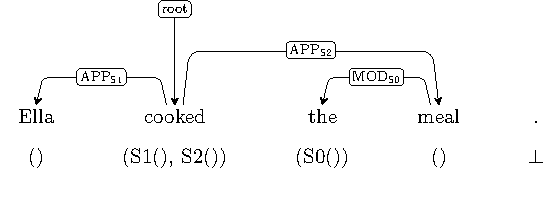
\includegraphics[scale=1.2]{figures/AM_dep_tree.pdf}
        \vspace{-1cm}
    \end{subfigure}

    \begin{subfigure}[t]{0.99\textwidth}
        \centering
        \vspace{-2cm}
        \raisebox{4\totalheight}{(b)}\phantomsubcaption\label{fig:b} 
        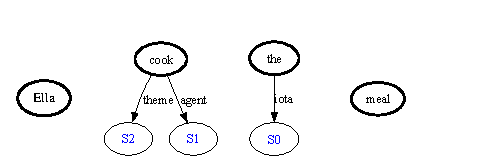
\includegraphics[scale=1.4]{figures/AM_supertags.pdf}
    \end{subfigure}
    \caption{Example of an AM dependency tree: (\subref{fig:b}) displays the supertags assigned to each token, while (\subref{fig:a}) presents the dependency tree connecting them.}
    \label{fig:supertag_example}
\end{figure}

To provide a valuable point of comparison, we finally evaluate a structure-informed model: AM-Parser \citep{groschwitz-etal-2018-amr}, which achieves near-perfect accuracy on COGS \citep{weissenhorn-etal-2022-compositional}. This allows us to measure how closely Transformer-based models can approximate the performance of a parser that explicitly incorporates compositional biases. Previous work has shown that structure-informed models perform well on compositional generalization tasks, specifically those involving structural generalization \citep{yao-koller-2022-structural}. Following \citet{weissenhorn-etal-2022-compositional}, we first have the AM-Parser predict an intermediate dependency tree (as shown in Figure~\ref{fig:supertag_example}), and then convert it to a graph-based representation of the SLOG logical form. The AM dependency tree labels each token with a \emph{supertag}, a small graph as illustrated in Figure~\ref{fig:b}, which captures the lexical meaning of each word. The tree's edges (Fig.~\ref{fig:a}) represent the compositional structure of the sentence, which specifies how the meaning of the sentence is recursively computed from the supertags.
For example, the second supertag in Figure~\ref{fig:b} represents the meaning of \textit{cooked} in the sentence \textit{Ella cooked the meal}. The blue markers ``S1'' and ``S2'' indicate that two arguments are needed to fill the agent and theme roles of \textit{cook}.

We use the A* AM-parser from \citet{lindemann-etal-2020-fast} for our experiments, as it yields the best overall results compared to alternative versions of AM-parser, such as the one in \citet{groschwitz-etal-2018-amr}.\footnote{For a more detailed discussion on alternative AM-parser models, please refer to Section~\ref{subsec:am_parser_analysis}.}

\vspace{-0.5\baselineskip}
\paragraph{Hyperparameters} 
The architecture of the vanilla Transformer model is the same as in original COGS, which consists of 2 encoder and 2 decoder layers, 4 attention heads per layer, and a feedforward dimension of 512. We use the best combination of hyperparameters from \citet{csordas-etal-2021-devil} on COGS: a learning rate of 0.0001 with no label smoothing, warmup, or early stopping. Absolute positional embeddings with down scaling scheme \citep{he2015delving,csordas-etal-2021-devil} is used due to stability issues observed with relative positional embeddings in recursive depth generalization cases, a similar phenomenon also noted in Csordas and colleague's experiments. Models are trained for 50k steps with a batch size of 128.

For the T5 experiments, we finetune T5-base\footnote{\url{https://huggingface.co/t5-base}} using a learning rate of 1.5e-5 and no label smoothing, warmup or early stopping. We finetune the model for 50k steps using a batch size of 2048.

For the LLaMA experiments, we finetune \texttt{llama-7b-hf} with LoRA \cite{hu2021lora}.\footnote{Low-Rank Adaptation of Large Language Models: \url{https://github.com/tloen/alpaca-lora}} We set the learning rate to 3e-4, LoRA rank to 8, alpha to 32 and dropout to 0.1. We finetune the model for 5K steps with a batch size of 64, with 100 warmup steps and no label smoothing or early stopping. We apply LoRA to ${W_q}$ and ${W_v}$ weight matrices in the model.

All our experiments were run five times, using different random seeds. The final checkpoints from each run were used for evaluation on both the in-domain test and out-of-domain generalization sets.

\subsection{Evaluation metric} 

Most studies report exact match accuracy on COGS. This metric has two limitations that may lead to an underestimation of a model's generalization capacity. First, because the COGS LF is conjunctive, any reordering of the conjuncts are semantically equivalent; yet, under exact match accuracy, only a single order is considered correct. Second, the COGS LF uses Skolem constants with a naming scheme tied to the linear indices of phrasal heads in the input. For example, in (\ref{ex:eval_ori_gold}), the constant saturating \lform{baby} is $x_3$ because, assuming 0-indexing, \textit{baby} appears in linear position 3 of the English expression \textit{What did the baby eat?}. While a commitment to a systematic naming scheme is necessary for consistent evaluation, different naming schemes up to the renaming of the constants in the gold LF yield equivalent LFs (e.g., (\ref{ex:eval_ori_gold}) vs. (\ref{ex:eval_ori_pred})). Such LFs would be considered incorrect under exact match.

To incorporate semantic equivalence up to conjunct reordering and constant renaming, at evaluation time, we alphabetically sort the conjuncts of the gold LFs, and subsequently index variables based on their appearance order in the sorted LFs. The same modifications are applied to the model output. This process results in the reformatted output as shown in (\ref{ex:eval_re}); applying these modifications to (\ref{ex:eval_ori_gold}) and (\ref{ex:eval_ori_pred}) yields the same outcome. Then, computing the exact match on these postprocessed LFs captures the targeted semantic equivalence.

\vspace{-0.5\baselineskip}
\begin{exe}
\ex \label{ex:eval_ori} Gold LF and model-predicted LF for \textit{What did the baby eat?}:
    \begin{xlist}
        \ex \label{ex:eval_ori_gold} Gold: \lform{eat.theme (x\textcolor{red}{$_4$}, ?) $\land$ eat.agent (x\textcolor{red}{$_4$}, x\textcolor{blue}{$_3$}) $\land$ baby (x\textcolor{blue}{$_3$})}
    \ex \label{ex:eval_ori_pred} Out: \lform{eat.agent (x\textcolor{red}{$_3$}, x\textcolor{blue}{\textcolor{blue}{$_6$}}) $\land$ eat.theme (x\textcolor{red}{$_3$},?) $\land$ baby(x\textcolor{blue}{\textcolor{blue}{$_6$}})}
    \end{xlist}
\ex \label{ex:eval_re} Re-indexed and re-ordered version: 
    \begin{xlist}
        \ex \lform{baby (y$_2$) $\land$ eat.agent (y$_1$, y$_2$) $\land$  eat.theme (y$_1$, ?)}  	
    \end{xlist}
\end{exe}
\vspace{-0.5\baselineskip}
\noindent This reformatted exact match metric is used for all results reported in the main text; see Appendix~\ref{app:metric} and Table~\ref{tab:res_cases} for more details. 

\section{Results} \label{sec:slog_res}

Overall, seq2seq Transformers, both trained from scratch and pretrained, display low accuracy on SLOG (Figure~\ref{fig:slog_cogs_res}), in line with earlier studies on structural generalization in seq2seq models \citep{yao-koller-2022-structural}. This is also the case for the more recent autoregressive Transformer LLaMa, whose performance is similar to that of T5. 



\begin{figure}[htbp]
  \centering
  \vspace{-4mm}  % reduce space above the figure
    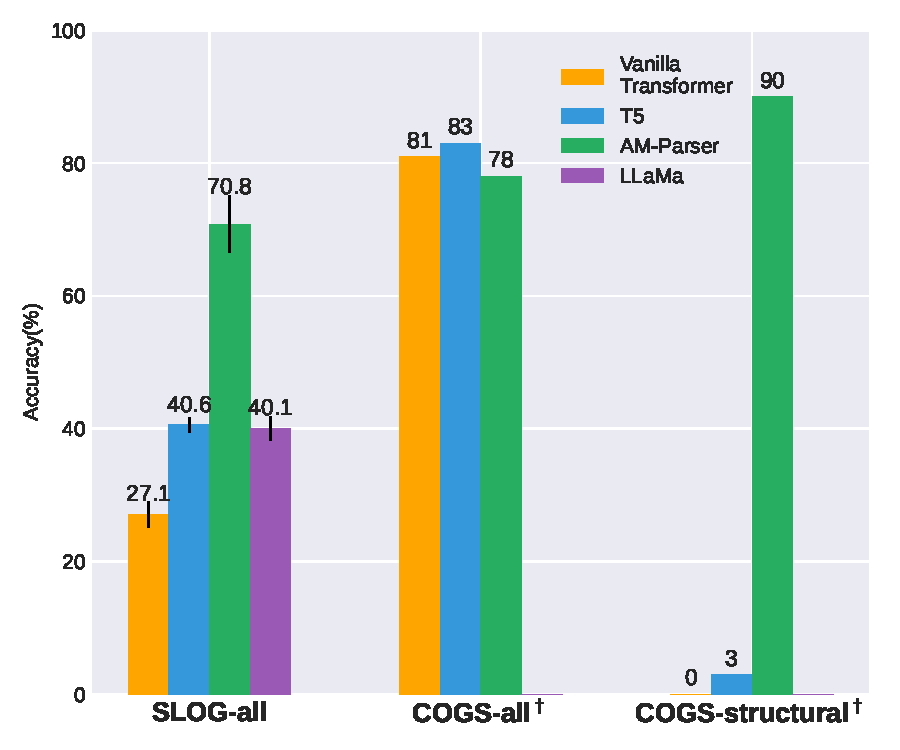
\includegraphics[scale=0.75]{figures/res_overall_slog_cogs.pdf}
    \vspace{-1mm} 
    \caption{Accuracy on SLOG, with error bars indicating variations across five runs. We also show the best published results on COGS (indicated with $^\dagger$), as reported in \citet{yao-koller-2022-structural}.}
    \label{fig:slog_cogs_res}
    \vspace{-2mm}  % reduce space below the figure
\end{figure}

\begin{figure}[H]
  \centering
  \vspace{-3mm} 
    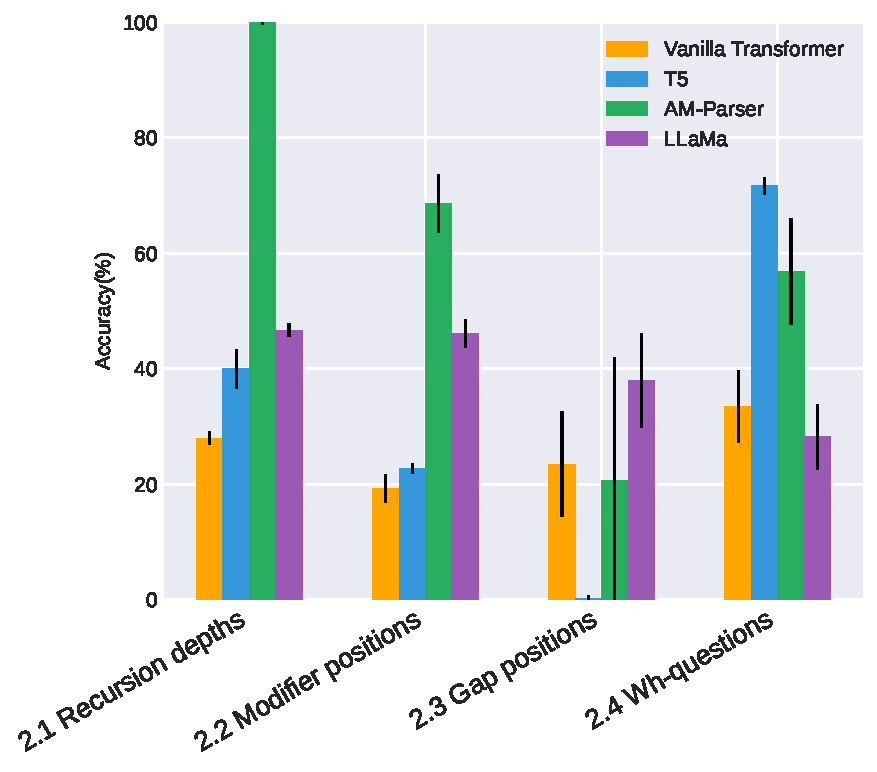
\includegraphics[scale=0.85]{figures/res_accuracy_category.pdf}
    \vspace{-1mm} 
    \caption{Aggregate accuracy on SLOG by generalization category, with error bars denoting the variations across generalization cases within each category over five model runs.}
    \label{fig:res_category}
    \vspace{-3mm} 
\end{figure}
 

As Figure~\ref{fig:slog_cogs_res} shows, high accuracy on the full COGS dataset, where 86\% of the generalization cases are lexical, can obscure low performance on structural generalization, highlighting the need for the expanded structural generalization tests included in SLOG.

SLOG additionally reveals weaknesses in the AM-Parser that COGS did not. While AM-Parser achieves 90\% accuracy on the structural generalization subset of COGS (Figure~\ref{fig:slog_cogs_res}), it faces systematic difficulties with several generalization types introduced in SLOG (Figure~\ref{fig:res_category}). We provide a detailed discussion of these difficulties in Section~\ref{subsec:am_parser_analysis}. 


Performance varied substantially across generalization categories (Figure~\ref{fig:res_category}); in particular, all models achieve near-perfect accuracy on \textit{Active subject wh-questions} and \textit{Shallower PP recursion}. These cases were the least structurally complex in their respective categories (\S\ref{subsec:cat_gap} and \S\ref{subsec:cat_recur}). 
We highlight several error patterns in individual generalization cases in more detail in the remainder of this section; see Appendix~\ref{sec:analysis_case} for full results and additional error analysis.


\subsection{Unobserved depth and length both affect depth generalization} \label{subsec:depth_gen}

The maximum depth observed in training was four levels of embedding for all three recursive structures tested. All models achieve greater than 90\% accuracy on unseen shallower PP recursion (three levels of embedding). A considerable lower performance is observed for Seq2Seq models with shallower tail CP recursion (<61\%); in particular, the vanilla Transformer consistently fails to generalize to shallower center embedding, with zero accuracy overall. Transformer models show systematically lower performance on deeper recursions (5-12 levels of embedding), whereas the structure-informed parsing model is robust to depth variation. 

\begin{table}[ht]
    \centering
    \begin{tabular}{lcccc}
    \toprule
     & \makecell[c]{Vanilla \\ Transformer} & T5 & LLaMa & \makecell[c]{AM \\parser} \\
    \midrule
     \textit{Within max training length}  &&&\\
    PP recursion & 29.3 &37.0 &46.0& 100.0 \\
    Tail CP recursion & 3.0 & 17.7&40.2& 100.0\\
    Center embedding & 0.0 & 0.0 &0.0& 100.0\\
    \midrule
    \textit{Beyond max training length }  &&&\\
    PP recursion & 0.0 &0.0 &0.0&100.0 \\
    Tail CP recursion & 0.0 & 0.0&0.0&100.0\\
    Center embedding & 0.0 &0.0&0.0&100.0 \\
    \bottomrule
    \end{tabular}
    \caption{Mean accuracy (\%) on unseen deeper recursion cases within and beyond the range of training output lengths (maximum training output = 229 tokens).}
    \label{tab:res_recursion}
\end{table}

We investigate the relation between length and depth generalization further by dividing the deeper depth generalization cases into examples that are shorter vs. longer than the maximum output length observed in training (229 output tokens). Results are shown in Table \ref{tab:res_recursion}. Both the vanilla Transformer and two pretrained  models are unable to generalize to examples longer than the maximum output length observed in training; this result is consistent with the difficulty of length extrapolation observed in the literature \citep{hupkes2020compositionality,anil2022exploring}. Length extrapolation does not capture the full story, however: their performance is limited even when the length of the generalization examples fall within the range of observed output lengths. This indicates that unobserved depth indeed plays a role in these models' poor generalization to deeper structures, in addition to known difficulties in length generalization.

\subsection{Unobserved long-distance dependencies make generalization difficult} \label{subsec:long_distance_hard}


Generalizing to subject modification (both PP and RC) is one of the most challenging cases in SLOG, Seq2seq models achieve near-zero accuracy, even with the additional cue from the standalone modified NPs that modification can appear outside of object positions. This challenge echoes previous findings on COGS \citep{akyurek-andreas-2021-lexicon,zheng-lapata-2022-disentangled,yao-koller-2022-structural}. The remainder of this subsection focuses on the analysis of PP modification cases, but similar patterns are observed for RC modifiers, which we discuss in Appendix \ref{app:RC_modifiers_results}.

Common error patterns across vanilla Transformer and two pre-trained models reveal a model bias towards shorter predicate-argument dependencies, which partly explains the difficulty of this generalization case. For instance, in sentences like \textit{A {\bf cat} on the mat {\bf froze}}, models often misinterpret the closer NP \textit{the mat} as the subject of \textit{froze}.

A further breakdown of the modifier generalization performance (Table~\ref{tab:cat_1_analysis}) illustrates the difficulty of long-distance dependencies clearly. As discussed in Section~\ref{subsec:cat_mod}, the sub-cases in indirect object modification feature predicate-argument dependencies of varying distance. We can see that generalization examples involving long predicate-argument dependency (i.e., there is an intervening non-argument NP between the predicate and the argument) tend to be more difficult for all models. However, the vanilla Transformer and pre-trained models show a stronger bias towards linearly adjacent predicate-argument structures.

\begin{table}[th]
    \centering
    \scalebox{0.85}{
    \begin{tabular}{lccccc}
      \toprule
       Generalization cases & \makecell[c]{Long pred-arg \\dependency?} & \makecell[c]{Vanilla \\Transformer} & T5 & LLaMa&\makecell[c]{AM \\parser}   \\
       \midrule
       \makecell[l]{ {\scriptsize Sub-case: Passive indirect objects} \\  \textbf{A fish} \textbf{was given} to  [ a cat on the mat ]$_{\textcolor{blue}{\bf iobj}}$. } & \ding{55}  & 95.5  & 97.5  & 98.2 & 93.6 \\
       \makecell[l]{ {\scriptsize Sub-case: Indirect object in PP datives  } \\   Emma \textbf{gave a fish} to  [ a cat on the mat ]$_{\textcolor{blue}{\bf iobj}}$.} & \ding{55} & 22.9  & 50.5 & 75.5 & 100.0  \\
      \makecell[l]{ {\scriptsize Sub-case: Indirect object in double object datives} \\    Emma \textbf{\textcolor{orange}{gave}} [ a cat on the mat ]$_{\textcolor{blue}{\bf iobj}}$ \textbf{\textcolor{orange}{a fish}}.} & \ding{51} & 4.5 & 9.7  &36.3 & 77.9 \\
      \makecell[l]{ {\scriptsize Subject} \\ \  [\textbf{\textcolor{orange}{A cat}} on a mat]$_{\textcolor{blue}{\bf subj}}$ \textbf{\textcolor{orange}{ate}} a fish. } & \ding{51} & 0.0 & 0.8 &28.9&57.6\\
      \bottomrule
    \end{tabular}    
    }
    \caption{Performance of PP modification generalization broken down by construction. Bold orange words denote long predicate-argument dependencies, while bold black words indicate short ones.} 
    \label{tab:cat_1_analysis}
\end{table}

For both constructions involving long predicate-argument dependencies, indirect object position seems less challenging than subject position. A possible explanation is that the former has a closer surface resemblance to direct object modification~---~modifiers attach to an immediate post-verb NP. Indeed, we observe that a higher proportion of indirect object modifications are partially correct; models correctly predicted the PP-modified NP, but erred in the argument structure. 

We furthermore note that the results in Table~\ref{tab:cat_1_analysis} also show lower performance of Transformer models for \textit{Indirect object in PP datives} compared to \textit{Passive indirect objects}, although neither subcase introduces long predicate-argument dependencies. The predominant error pattern in the former subcase is the incorrect attachment of PP modifiers to the direct object NP. For example in (\ref{ex:iobj_a_dobj_pred}), NP inside the modifier \textit{on the mat} denoted by \lform{$x_9$} was attached to \textit{a fish} instead of \textit{the cat}. This suggests that Transformers additionally apply the incorrect modification rule ``attach PPs to NPs in immediate post-verb position'', which is compatible with the training data but does not lead to correct generalization. 

\begin{exe}
\ex \label{ex:iobj_error} Gold LF and model-predicted LF for \textit{Emma gave a fish to the cat on the mat}:
    \begin{xlist}
        \small{
        \ex \label{ex:iobj_a_dobj_gold} Gold: \lform{*cat ($x_6$); *mat($x_9$); \\ give.agent ($x_1$,Emma) $\land$ give.theme ($x_4,x_3)$ $\land$  give.recipient ($x_1,x_6$)$\land$ fish($x_3$) $\land$ \textbf{cat}.nmod.on (x\textcolor{red}{$_6$}$,x_9$)}
    \ex \label{ex:iobj_a_dobj_pred} Out: \lform{*cat ($x_6$); *mat($x_9$); \\ give.agent ($x_1$,Emma) $\land$ give.theme ($x_4,x_3)$ $\land$  give.recipient ($x_1,x_6$)$ \land$ fish($x_3$) $\land$ \textbf{fish}.nmod.on (x$\textcolor{red}{_3},x_9$)}
    }
    \end{xlist}
\end{exe}


\subsection{Gap generalizations are challenging for all tested models} \label{subsec:am_parser_analysis}

All tested models encounter significant difficulties with gap constructions, as evidenced by their low accuracy and considerable variability across runs. In the case of indirect object-extracted relative clauses (\ref{ex:RC_iobj_extracted}), a common error pattern emerges across all models: they tend to mirror the training pattern of direct object-extracted RCs, as demonstrated by the incorrect output (\ref{ex:RC_iobj_extracted_error}). In contrast, when handling \emph{wh}-questions, the models show distinct difficulties, revealing varied error patterns.

\begin{exe}
    \ex \label{ex:RC_iobj_extracted} Input: Ella cooked the servant that Emma gave a tool to \_\_.
    \begin{xlist}
    \ex \label{ex:RC_iobj_extracted_gold} Gold: \lform{*servant($x_3$);cook.agent($x_1$, Ella) $\land$ cook.theme($x_1, x_3$) \\ $\land$  servant.nmod( $x_3, x_6$) $\land$ give.agent($x_6$, Emma) $\land$ give.theme ($x_6,\textcolor{blue}{x_8}$) \\ $\land$ 
    give.recipient($x_6,x_3$) $\land$ tool ($\textcolor{blue}{x_8}$)}
    \ex \label{ex:RC_iobj_extracted_error} Models output: \lform{*servant($\textcolor{red}{x_3}$);cook.agent($x_1$, Ella) $\land$ cook.theme($x_1, x_3$) $\land$ servant.nmod( $x_3, x_6$) $\land$ give.agent($x_6$, Emma) $\land$ give.theme ($x_6,\textcolor{red}{x_3}$) $\land$ give.recipient($x_6,x_8$) $\land$ tool ($x_8$)} 
    \end{xlist}
\end{exe}

\paragraph{Direct and indirect \textit{wh}-questions}The vanilla Transformer and LLaMa frequently misinterpret the theme role in direct object \emph{wh}-questions. For example, they often fail to map \emph{wh}-words to `?' as illustrated in (\ref{ex:q_error_tm}):  
\begin{exe}

\ex \label{ex:q_input}Input: What did Emma sell to Liam ?
%\vspace{-0.4em}
\small{\begin{xlist}
    \ex \label{ex:q_gold} Gold:\lform{sell.theme (x$_3$, ?)$\land$ sell.agent (x$_3$, Emma) $\land$ sell.recipient(x$_3$,Liam)}
    \ex \label{ex:q_error_tm} Output of vanilla Transformer and LLaMa: \\ \lform{sell.theme (x$_3$,  \textcolor{red}{x$_3$}) $\land$ sell.agent (x$_3$, Emma)$\land$ sell.recipient(x$_3$,Liam)}
    \ex \label{ex:q_error_am} AM parser's output: \\ \lform{sell.\textcolor{red}{agent} (x$_3$,  ?) $\land$ sell.\textcolor{red}{theme} (x$_3$, Emma)$\land$ sell.recipient(x$_3$,Liam)}
\end{xlist}}
\end{exe}

\noindent This error pattern can be traced back to frequency of the subsequences in the training data. Three types of tokens can appear post-comma in the output LF space: \lform{$x$}, \lform{?} (denoting \emph{wh}-words), or a proper noun (\lform{PropN}), such as \lform{Emma}. The subsequence \texttt{theme($x_i,x_j$)} is 20 times more frequent than \texttt{theme($x_i$,?)} and \texttt{theme($x_i$,PropN)}. This discrepancy does not affect all models equally; in fact, T5 can generalize correctly for some constructions despite this skewed label distribution, achieving near-perfect accuracy for direct object \emph{wh}-questions. However, when it comes to less frequent constructions --- indirect object \emph{wh}-questions, T5 overgeneralizes. In 94.6\% of these cases, it erroneously produces the observed direct object \emph{wh}-questions pattern \texttt{theme(x$_i$,?)}, instead of the correct but unseen \texttt{recipient(x$_i$,?)}. This observation aligns with the findings of \citet{wu2023recogs,yao-koller-2022-structural}, who noted that the decoder of Transformer models tends to exhibit a heavy bias towards generating observed $n$-grams.

\begin{figure}[ht] 
    \centering

    \begin{subfigure}[t]{0.99\textwidth}
        \centering
        \raisebox{4\totalheight}{\phantom{(abc)}}\phantomsubcaption
        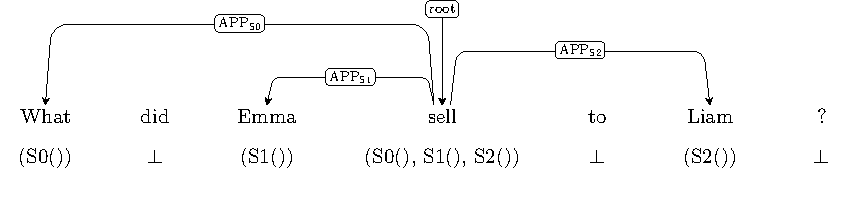
\includegraphics[scale=0.97]{figures/dobj_Q_deptree.pdf}
        \vspace{-1cm}
    \end{subfigure}
    \setcounter{subfigure}{0}  % Reset the subfigure counter
    \begin{subfigure}[t]{0.99\textwidth}
        \centering
        \vspace{-1.5cm}
        \raisebox{3\totalheight}{(a)}\phantomsubcaption\label{fig:dobj_Q_gold} 
        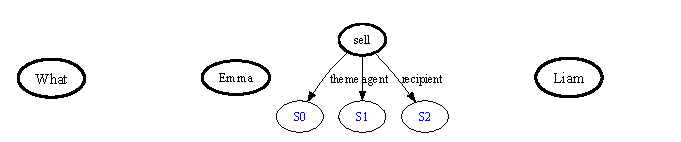
\includegraphics[scale=1.2]{figures/dobj_Q_gold_supertags.pdf}
    \end{subfigure}
    \begin{subfigure}[t]{0.99\textwidth}
        \centering
        \vspace{-0.5cm}
        \raisebox{3\totalheight}{(b)}\phantomsubcaption\label{fig:dobj_Q_error} 
        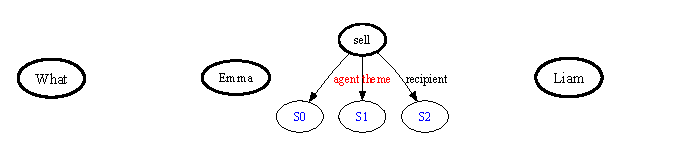
\includegraphics[scale=1.2]{figures/dobj_Q_error_supertags.pdf}
    \end{subfigure}
    \caption{AM dependency tree for a direct object \textit{wh}-question. (\subref{fig:dobj_Q_gold})  displays the gold supertags and (\subref{fig:dobj_Q_error}) shows the incorrect predicted supertags. }
    \label{fig:dobj_deptree}
\end{figure}


AM-Parser shows considerable fluctuation in performance across different runs on the indirect and direct object \textit{wh}-questions cases, with accuracies ranging from 0 to 80 depending on the random seed. This is because at the bottom of its compositional process, the AM-Parser predicts the lexical meaning for each token in the sentence (\textit{supertag}). In these generalization types, the gold meaning representations in the test set require supertags that are infrequent in training. 

We show an example of AM dependency trees for an \textit{direct object wh-question} sentence in Figure \ref{fig:dobj_deptree}, with gold supertags in Figure~\ref{fig:dobj_Q_gold} and predicated supertags in Figure~\ref{fig:dobj_Q_error}. The issue here is that the model predicts the wrong supertag for \emph{sell}, treating \emph{What} as its \texttt{agent} instead of \texttt{theme}, and \emph{Emma} as its \texttt{theme} rather than \texttt{agent}, which results in the erroneous output LF as shown in (\ref{ex:q_error_am}). The AM-Parser is limited to using supertags that it observed at training time (possibly with different node labels to accommodate novel lexical material). In this case, the correct supertag was actually present in the training data, but it was much less frequent than the one in Figure~\ref{fig:dobj_Q_error}. We conjecture that the AM-Parser was overly sensitive to the supertag distribution in the training data in this case, pointing to a further architectural limitation. 

Thus, while the AM-Parser can compensate the distribution shift of the meaning representations as a whole, SLOG exposes its weakness to distribution shifts in the lexical supertags. 





\paragraph{\textit{Wh}-questions with long movement} 
All models achieve very low accuracy when generalizing to longer filler-gap dependency across CPs.

In example (\ref{ex:q_long_mv_tm}), we show an example of a \textit{wh-question with long movement}, with its gold meaning representation (\ref{ex:q_long_mv_gold}) and the most common errors produced by Transformer-based models. As shown in (\ref{ex:q_long_mv_tm}), the vanilla Transformer commonly misinterprets the complementizer \textit{that} (corresponding to \texttt{ccomp} in the LF) as a relative pronoun (\texttt{nmod}). Additionally, it tends to interpret the \emph{wh}-word as the direct object of the CP verb, \emph{e.g., say}. In the most common errors for T5 and LLaMa (\ref{ex:q_long_mv_t5}), the whole gap conjunct (\lform{paint.theme($x_7,?$)}) is missing, revealing their difficulties in establishing long-range filler-gap dependencies between the initial \emph{wh}-word and the embedded gap position. 
 
\begin{exe}
\ex \label{ex:q_long_mv_input}Input: What did Liam say that the bear painted \_\_ ?
\begin{xlist}
    \ex \label{ex:q_long_mv_gold} Gold:  \lform{*bear(x$_6$); say.agent(x$_3$,Liam) $\land$ say.ccomp(x$_3$,x$_7$) $\land$ \\ paint.agent(x$_7$,x$_6$) $\land$ paint.theme(x$_7$,?)}
    \ex  \label{ex:q_long_mv_tm} Output of vanilla Transformer:  \lform{*bear(x$_6$); say.agent(x$_3$,Liam) $\land$ \\ \textcolor{red}{say.theme(x$_3$,?)} $\land$ say.\textcolor{red}{nmod}(x$_3$,x$_7$) $\land$ paint.agent(x$_7$,x$_6$) $\land$ \\ paint.theme(x$_7$,?)}
    \ex \label{ex:q_long_mv_t5} Output of T5 and LLaMa:  \lform{*bear(x$_5$); say.agent(x$_3$,Liam) $\land$ \\ say.ccomp(x$_3$,x$_7$) $\land$ paint.agent(x$_7$,x$_5$) }
\end{xlist}
\end{exe}

The AM parser fails on all test instances in the case of \textit{wh-questions with long movement}. We present a predicted AM dependency tree for such a sentence in Figure \ref{fig:predicted_Q_long_mv}, contrasted with the corresponding gold standard AM dependency tree in Figure \ref{fig:gold_Q_long_mv}. Notably, for \textit{wh}-questions with long movement, the required dependency trees are nonprojective, as illustrated in Figure \ref{fig:gold_Q_long_mv}: the edge from the embedded verb to the \textit{wh}-pronoun (the edge \texttt{snapped -> Who}) crosses the matrix verb (\texttt{root -> appreciate}). However, the A* AM-Parser used in our study only supports projective dependency trees, leading to incorrect prediction of sentence structure as shown in Figure \ref{fig:predicted_Q_long_mv}.\footnote{Instead of the A* parser, one could instead use the fixed-tree decoder of \citet{groschwitz-etal-2018-amr}, which is capable of predicting non-projective
AM dependency trees. This parser achieves nonzero accuracy (36\%) on \textit{wh}-questions with long movement,
confirming our hypothesis that the projectivity is the issue. However, the A* parser
outperforms the fixed-tree decoder on most other generalization types, which is why
we only report its results in the main body of the paper. The transition-based
AM-Parser of \citet{lindemann-etal-2020-fast} can also predict non-projective trees,
but uses a different probability model that is incompatible with the training algorithm
of \citet{groschwitz-etal-2021-learning} that we use here.}

\begin{figure}[ht]
    \centering
    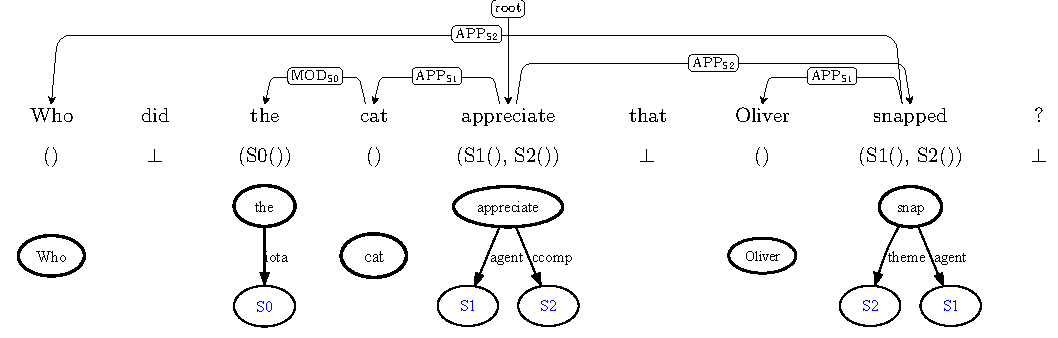
\includegraphics[scale=0.85]{figures/am_deptree_Q_long_mv.pdf}
    \caption{Example of gold AM dependency tree for \textit{wh}-questions with long movement}
    \label{fig:gold_Q_long_mv}
\end{figure} 

\begin{figure}[ht]
    \centering
    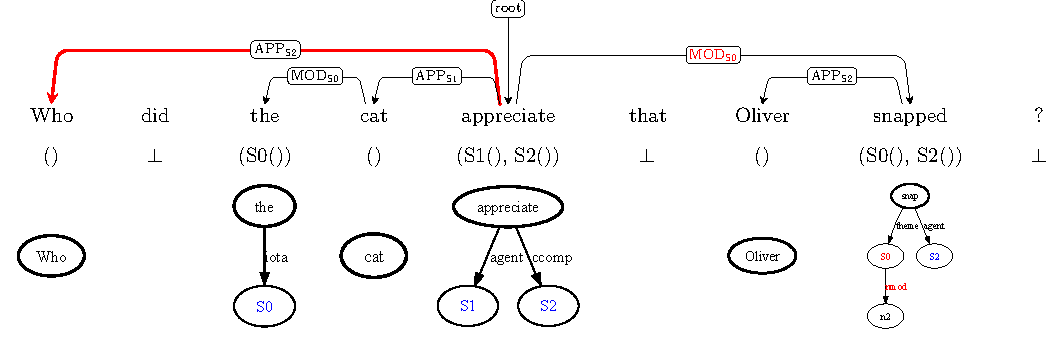
\includegraphics[scale=0.85]{figures/am_deptree_Q_long_mv_error.pdf}
    \caption{Example of predicted AM dependency tree for \textit{wh}-questions with long movement}
    \label{fig:predicted_Q_long_mv}
\end{figure} 


Note that the A* AM-Parser's limitation to projective structures is shared by many other compositional semantic parsers. For instance, the LeAR model of \citet{liu-etal-2021-learning-algebraic} uses phrase-structure trees as compositional structures. Similarly, the CSL-T5 parser of 
\citet{qiu-etal-2022-improving} uses phrase-structure trees during the data augmentation process. Since phrase structure trees are equivalent to projective dependency trees, these parsers are likely to encounter similar difficulties on SLOG.
Thus, this specific type of generalization can serve as a diagnostic tool to identify structural limitations in compositional semantic parsers.

\clearpage
\section{Conclusion} \label{sec:slog_conclu} 

Transformer-based models, despite lacking explicit symbolic representation, have demonstrated a remarkable ability to acquire nuanced syntactic representations, enabling them to handle structure-sensitive phenomena effectively, as discussed in Chapter~\ref{chp:main_project}. To further probe the extent to which their performance is driven by genuine syntactic generalization, aligned with symbolic compositional rules, as opposed to relying on structural similarity-based memorization derived from their training data, we introduced SLOG. This semantic parsing challenge set expands upon the COGS benchmark, and specifically targets structural generalization, which is often underrepresented in current compositional generalization benchmarks. 

Using SLOG, we assessed the structural generalization capacity of Transformer models (both pretrained and trained from scratch), as well as AM-Parser, a structure-informed parsing model. While all models achieve good overall accuracy on COGS ($\geq$ 78\%), their performance on SLOG is substantially lower. This was particularly evident for Transformer models, which scored below 41\%, lagging behind the structure-informed parser (70.8\%) by a wide margin. This performance discrepancy between SLOG and COGS illuminates the notable gap between models' lexical and structural generalization abilities. 

Prior studies have shown that RNN models often struggle with learning complex long-range relations from simpler formal languages \citep{avcu2017subregular, mahalunkar-kelleher-2019-multi}. Our results on SLOG reveal that unseen long-distance predicate-argument dependencies pose considerable difficulty for Transformer-based models as well (\S\ref{subsec:long_distance_hard}). 
Additionally, these Transformer models struggle with deeper recursive constructions. Our results corroborate the observations of \cite{hupkes2020compositionality} and \cite{lakretz2021can}, and further highlight challenges posed by unobserved deeper patterns, which persist beyond the recognized issue of length extrapolation~(\S\ref{subsec:depth_gen}). On the other hand, the AM-Parser, despite its stronger overall performance (70.8\%), displays categorical failures on gap generalization due to its inherent parser design limitations (\S\ref{subsec:am_parser_analysis}). 

These findings underscore the utility of SLOG in exposing the limitations of current semantic parsing models, which have previously been claimed to achieve good compositional generalization. SLOG thus can serve as a useful analytic tool for guiding future improvements. Furthermore, these results indicate that while Transformer-based models can approximate compositional behavior to a certain extent, they do not seem to rely on the kind of syntactic generalization rooted in systematic compositional rules. This insight lends support to the hypothesis that the Transformer model's ability to leverage hierarchical structures for nuanced syntactic generalization, as explored in Chapter~\ref{chp:main_project}, might be more attributable to structural similarity-based analogies at the lexico-categorical abstraction level, rather than the internalization and application of systematic grammatical rules. This enables the models to handle a sophisticated form of language productivity; however, they falter when faced with novel linguistic structures that require the induction of systematic compositional rules.

The evaluation conducted with the SLOG challenge set represents only the first step --- behavioral level --- of our integrated three-level analysis framework as detailed in Chapter~\ref{chp:main_project}. This study thereby lays the groundwork for future research, particularly aimed at understanding what makes structural generalization so hard for Transformer models. The logical progression would be to advance to the representational and functional levels of analysis, using probing classifiers and causal intervention methodologies to delve into the model's difficulties with SLOG. 

\stopcontents[chapters]
\part{Conclusion}
\chapter{Conclusions and perspectives}
%\startcontents[chapters]
%\addcontentsline{toc}{chapter}{Conclusions and perspectives}  

\section{Conclusions}

This dissertation explored the abstraction capabilities of Transformer language models for syntactic processing. We sought to determine if these models rely mainly on surface-level patterns from their training data, or if they also implicitly construct abstract syntactic rules. Our research had two main objectives: first, to assess the potential of the autoregressive Transformer model as an explanatory tool for human syntactic processing; and second, to enhance interpretability methods for Transformer-based models. 

Our research makes two main contributions. First, we have introduced an integrated framework for assessing the linguistic capacities of Transformer-based models. Second, we applied this framework to evaluate the models on two aspects of syntactic abstraction: the capacity to represent hierarchical structures and the capacity to compositionally generalize observed structures. These evaluations conducted align closely with the key prerequisites specified in Section~\ref{sec:research_Q}, which are essential for a computational model to serve as a credible explanatory tool for human language processing. Our findings reveal that Transformers manage to represent hierarchical structures for nuanced syntactic generalization. However, instead of relying on systematic compositional rules, they seem to lean more towards lexico-categorical abstraction and structural similarity-based analogies~(\S\ref{chp:slog}).  
This study both highlights the potential of autoregressive Transformer models as explanatory tools for human syntactic processing and provides a methodological framework for their analysis and interpretability.


From a methodological standpoint, we introduce a comprehensive linguistically-informed analysis framework that builds upon and enhances recent interpretability techniques. The framework operates on three interrelated levels. First, behavioral assessment, grounded in challenge sets that target specific syntactic phenomena, serves as the foundational layer. This level assesses whether the model meets the requirement of reflecting human grammatical behavior. Although it reveals how the model behaves in response to certain inputs, it provides limited insight into its internal representations. Addressing this, the next level uses probing classifiers to locate the distribution of relevant syntactic information within the models. With these patterns identified, we introduce causal interventions as the third layer to decipher the underlying mechanisms driving a model's behavior and to evaluate their alignment with established linguistic analyses. This sets the stage for eventually modulating the model's behavior by tweaking the core components. In essence, our methodological framework serves two primary functions: it transforms linguistic theories into actionable, testable hypotheses, and enhances our ability to interpret and even guide Transformer-based models. In doing so, this framework takes a step toward fulfilling the `interpretability and controllability' criteria, essential for using Transformers to explain human language processing (\S~\ref{sec:research_Q}).


Our findings were twofold. First, our results in Chapter~\ref{chp:main_project} indicate that the Transformer model acquires remarkably nuanced representations of sentence structure, as evidenced by its strong performance on both behavioral-level tasks and measures of representational adequacy. Specifically, we curated challenge sets for subject-verb agreement across relative clauses and object past-participle agreement, which differ fundamentally in linguistic analysis despite their surface similarity. We then assessed whether the Transformer forms distinct representations for resolving these two agreements. Our heuristic-based evaluation in Section~\ref{sec:heuristics} highlights the model's strong ability for nuanced, structure-dependent generalizations that go beyond mere surface heuristics. Further exploration using probing classifiers~(\S\ref{sec:probing_location}) shows that syntactic information is mainly linearly encoded across all token representations between the two agreeing elements within a sentence. Despite this similar agreement information distribution pattern for both types of agreement, causal interventions experiments (\S\ref{sec:causal}) indicate that the model's predictions rely on linguistically relevant cues. These cues exhibit distinct patterns for different agreement phenomena, consistent with theoretical expectations. This evidence suggests that the autoregressive Transformer LM aligns with the key prerequisites for behavioral similarity and representational adequacy, as outlined in Section~\ref{sec:research_Q}. Along with our interpretability framework, this makes the model a promising tool for studying human syntactic processing.


Our second set of findings in Chapter~\ref{chp:slog} presents a contrasting narrative. When subjected to the SLOG tasks, designed to assess compositional generalization, Transformer models encountered significant difficulties. SLOG involves a semantic parsing task (i.e., mapping linguistic expressions to meaning representations).
The test is designed to have a systematic shift between training and evaluation sets, ensuring that success in the latter demands a level of compositional generalization. In this phase, we evaluated various Transformer models as well as a symbolic neural parser. While all models excelled in the in-domain test set, Transformer models, even the recent pre-trained ones, struggle to generalize to sentences with longer dependency and deeper levels of recursion --- areas where the symbolic parser performs much better. This divergence from human-like generalization, which allows for the interpretation of unfamiliar frames by systematically recombining known structures, suggests that Transformer models may rely on different or possibly insufficient underlying mechanisms.



The contrasting conclusions from Chapter~\ref{chp:main_project}, which highlights the model's proficiency in approximating hierarchical structures, and Chapter~\ref{chp:slog}, which underscores its limited compositional generalization capacity, paint a nuanced picture of Transformer models' syntactic abstraction capabilities. This suggests that Transformer-based models primarily rely on lexico-categorical abstraction and structural similarity-based analogies for syntactic representation. While this enables them to generalize over unseen sentences with familiar structures, thus handling a sophisticated form of grammatical productivity, they struggle to handle novel linguistic structures that require inducing systematic compositional rules. These results corroborate previous findings with RNN~\citep{baroni2020linguistic} and offer further empirical evidence that NLMs can achieve a certain level of abstraction for grammatical productivity without being truly compositional. Overall, this study highlights both the promise and potential limitations of autoregressive Transformer models as explanatory tools for human syntactic processing, and provides a methodological framework for its analysis and interpretability.

From a linguistic and cognitive science perspective, our positive results regarding the Transformer model's ability to represent hierarchical structures challenge the theory of syntactic nativism, which emphasizes innate structural properties. Our research reveals that an autoregressive Transformer language model, when exposed to human-scale learning data and trained merely to predict subsequent words, can grasp the intricacies of hierarchical-sensitive phenomena. This implies that the complexity of human syntactic competence could potentially be derived from exposure and general-purpose learning alone, without relying on innate linguistic priors. In this context, the Transformer model can set plausible lower bounds on the learnability of such abstractions, and provide a comparative baseline for understanding human syntactic processing. 

These positive results, coupled with the limitations observed in models' compositional structural generalizations, indicate that Transformer models can achieve structure-dependent generalization without systematically following compositional rules. Instead, they seem to rely mainly on lexico-categorical abstraction and analogies based on structural similarity. This provides constructive hypotheses about the learning and implementation of linguistic structure. On the other hand, while symbolic rules and recursive structures have traditionally been viewed as fundamental to our understanding of human language processing, they might not be the sole mechanisms for effective language processing. In particular, natural languages host many productive linguistic phenomena that follow less compositional, more complex principles, such as linguistic idiosyncrasies~\citep{dankers-etal-2022-paradox}, irregular inflections, and semi-lexicalized syntactic constraints~\citep{goldberg2004english}. Moving forward, investigating how Transformer models handle these phenomena could shed light on potential alternative cognitive strategies that remain underexplored in both human cognition and machine learning, presenting novel perspectives on computational approaches for linguistic productivity beyond the conventional rule-based compositionality. 
 

From a deep learning perspective, our research highlights both the capabilities and limitations of data-driven neural models like Transformers. While excel in tasks where vast amounts of data guide them, they seem to struggle when faced with genuine structural and compositional challenges. This prompts the question: Can we enhance the compositional capabilities of these models to boost their learning efficiency without scarifying generality? Current research trends point in this direction, with a focus on harnessing the intrinsic nature of language to refine neural network architectures. Recent efforts, such as the study of ~\cite{smolensky2022neurocompositional} on neurocompositional computing, suggest that by merging Compositionality and Continuity principles, there is potential to bridge the gap between symbolic and neural paradigms, pushing neural language models towards more robust compositional generalization. The SLOG test we developed (\S\ref{chp:slog}) can be a valuable tool to measure progress and guide model development. Crucially, by aligning models with compositional principles, we move closer to mirroring human cognitive processes, which could enhance their role as tools for understanding human language processing.



\section{Future work}
This dissertation highlights the potential of autoregressive Transformer language models as explanatory tools for the theoretical study of language and human linguistic processes. We introduced a methodological framework that facilitates testing linguistic hypotheses and conducting comparative studies between model behavior and human cognition. The next logical progression is to employ the model as an explanatory tool for human syntactic processing.

\paragraph{Autoregressive Transformer model as an explanatory tool for language processing:}
One direction that we initially aimed to explore in my thesis was the comparative analysis between human judgment and neural model behaviors on the two target agreement phenomena. While we have touched upon this topic preliminarily, a detailed study has not yet been conducted due to time limitations. Psycholinguistic studies have shown that humans also make agreement errors, with plural attractors being particularly error-prone. This is traditionally attributed to the markedness of plurals, whose features are more salient than the unmarked singular form during human language processing~\citep{BOCK199145,eberhard2005making}.
Our evaluation of neural language models on number agreement tasks (\S\ref{sec:h_eval_protocol}) revealed that performance drops with increasing sentence complexity (quantified by the heuristic count). This leads to pertinent questions: Do the patterns of errors echo between models and humans? Are human judgments also influenced by surface-level heuristics? Moreover, as detailed in Section~\ref{subsec:nonce_exp}, while models exhibited the capacity to extrapolate syntactic generalization even in semantically implausible contexts, one wonders: To what extent are rules governing linguistic structures separate from those guiding linguistic meanings?

Additionally, there is an evident human tendency to produce more accurate agreement when dealing with singular controllers\footnote{Controllers correspond to ``cues'' in our dissertation.} \citep{villata2017intervention}. This asymmetry is often linked to an inherent human bias towards producing default singular forms \citep{greenberg1963some,corbett2000gender}. Notably, our observations in Section~\ref{sec:freq_effects} reveal a similar singularity-plurality asymmetry within neural language models, with potential roots in the frequency-based biases of target verbs. This observation triggers a set of compelling inquiries: How does this resonate with established biases in the human cognitive system?
How do humans navigate and extract generalities from their linguistic stimuli? And, importantly, can the autoregressive Transformer language model shed light on the origins of these behaviors, especially when we manipulate model training data --- like data quantity, sentence structure complexity, and verb frequencies?

Another promising avenue for future research is to correlate model predictions with behavioral data. Number agreement tasks (\S\ref{chp:NA_tasks}) demonstrate how the outputs of the autoregressive language model can be directly used through minimal-pair comparisons. Another approach in the literature involves using the surprisal metric, calculated as the log of the inverse of the conditional word probability~\citep{hale2001probabilistic,levy2008expectation}. Given that in psycholinguistics, a word's surprisal linearly affects the reading time of native speakers~\citep{goodkind2018predictive,hale2001probabilistic}, using surprisal as a linking function allows comparisons between model output and human reading behavior, facilitating the testing of linguistic and cognitive theories. This could, for example, offer insights into the parallels between the Transformer model's attention mechanism and human working memory during reading tasks. Recent integrative modeling approaches, such as the one by~\cite{schrimpf2021neural}, linked neuropsychological data, behavioral responses, and computational model predictions. This establishes connections between neural activations, human responses to linguistic stimuli, and model-based surprisal values. Such endeavors can enhance our understanding of human language processing and refine our computational models to align more closely with human cognition.


\paragraph{Model interpretability} 
To effectively leverage Transformer language models for explaining human language processing, there is a pressing need to further illuminate their inner workings. Our framework, rooted in linguistic analysis, employs challenge sets, probing, and causal intervention methodologies. Yet, many interpretability methods lie outside the scope of our current exploration in this dissertation. 

A notable direction for further exploration is the neural-level analysis techniques, as detailed in the survey by~\cite{sajjad-etal-2022-neuron}. These techniques shed light on how models organize, specialize, and redundantly store knowledge, aligning well with our objectives. For instance, \cite{bau2018identifying} and ~\cite{dai-etal-2022-knowledge} have demonstrated how understanding neurons can help control the output of a model. Furthermore, such a granular understanding can guide the optimization of model architectures, possibly minimizing the required parameters~\citep{voita-etal-2019-analyzing,sajjad2004poor,dalvi-etal-2020-analyzing}. Aligning these capabilities with our objective can reinforce the potential of Transformer models as explanatory tools for human linguistic behaviors.

In Chapter~\ref{chp:slog}, we highlighted the challenges faced by Transformer models in compositional structural generalization. As a future endeavor, we aim to understand what makes compositional generalization difficult for NLMs. Specifically, how do Transformer models combine token-based information into representations for larger linguistic structures? Additionally, exploring recent hybrid methodologies, which blend symbolic and neural network paradigms, appears promising, for instance, neurocompositional computing by~\cite{smolensky2022neurocompositional}.

% Add the bibliography to the table of contents as a chapter
\addcontentsline{toc}{chapter}{Bibliography}
\bibliography{anthology,custom}
\bibliographystyle{acl_natbib}


%\paragraph{Résumé (long) :} 
\chapter*{Résumé}
\addcontentsline{toc}{chapter}{Résumé} 
Les théories linguistiques supposent que la compétence linguistique humaine est fondée sur des structures innées et des représentations symboliques~\citep{chomsky1965aspects,chomsky1986knowledge}. Cependant, les modèles de langues basés sur le Transformeur, sans intégrer explicitement ces principes, ont atteint des performances comparables à celles de l'être humain dans de nombreuses tâches de traitement automatique de langues (TAL)~\citep{lertvittayakumjorn2021explanation,bubeck2023sparks}. Contrairement aux modèles traditionnels basés sur l’apprentissage supervisé et des représentations symboliques tels que les arbres syntaxiques, les Transformeurs apprennent leur représentation du langage directement à partir de textes bruts, sans guidance grammaticale. Ce succès remet en question l'importance des structures hiérarchiques en traitement du langage, et suscite également des interrogations sur les mécanismes qui sous-tendent la compétence linguistique des Transformeurs. Une question clé, qui est également le cœur de cette thèse, est de savoir si les Transformeurs construisent implicitement une forme de représentation hiérarchique abstraite.  La complexité de ces modèles, avec leurs nombreux paramètres, rend difficile la compréhension de leur fonctionnement interne. Bien que la recherche dans ce domaine soit en plein essor, l’étendue de la capacité d’abstraction linguistique des Transformeur reste une question ouverte. Certains travaux soulignent la compétence du modèle à capturer des nuances syntaxiques complexes, tandis que d’autres suggèrent une possible dépendance excessive à des régularités statistiques ou une simple mémorisation des données. Cette thèse vise à éclaircir si les Transformeurs représentent principalement des structures syntaxiques à travers des motifs de surface ou s'ils forment également des règles plus abstraites. En abordant cette question, nous cherchons à explorer les niveaux d'abstraction syntaxique que ces modèles peuvent atteindre et les mécanismes qui guident leurs prédictions. L'étude poursuit deux objectifs principaux : i) évaluer le potentiel d'un modèle de langue Transformeur autorégressif comme outil explicatif pour le traitement syntaxique humain ; ii) améliorer l'interprétabilité du modèle.

Nous abordons ces objectifs en examinant les abstractions syntaxiques des modèles Transformeur sur deux niveaux : leur capacité à modéliser des structures hiérarchiques, présentée dans le Chapitre~\ref{chp:main_project}, et leur capacité à généraliser de manière compositionnelle les structures apprises, exposée dans le chapitre~\ref{chp:slog}. Ces deux aspects sont essentiels à la cognition linguistique humaine. Notre étude se concentre sur le modèle de langue Transformeur autorégressif, car son objectif de modélisation du langage est en phase avec la prédiction incrémentale des mots, caractéristique fondamental du traitement linguistique humain~\citep{hale2001probabilistic,kuperberg2016we,levy2008expectation}

Nous avons introduit un cadre d'analyse intégré comprenant trois niveaux interdépendants: évaluation comportementale à travers des ensembles de test de défis, analyse représentationnelle à l'aide de sondes linguistiques, et analyse fonctionnelle par intervention causale. Dans le chapitre~\ref{chp:main_project}, nous avons déployé ce cadre pour mener une étude contrastive sur la capacité du modèle Transformer à représenter des structures hiérarchiques. L’étude se focalise sur deux phénomènes d’accord à longue distance en français : l'accord sujet-verbe à travers des propositions relatives (S-V désormais) illustré par (\ref{ex:agrS_abs}), et l'accord objet-participe passé (O-PP désormais) illustré par (\ref{ex:agrO_abs}).

\setcounter{exx}{0} % Start numbering examples from 1
\vspace{-0.8\baselineskip}
\begin{exe}
   \ex\label{ex:agrS_abs}
    Les \textbf{chat·s} [ que Noûr aime bien
  ]\textcolor{blue}{$_{RC}$} \textbf{jou·ent} dans le jardin. 
  \vspace{-0.2\baselineskip}
   \ex\label{ex:agrO_abs}
   Les \textbf{chat·s} [ que Noûr a \textbf{adopté·s} ]\textcolor{blue}{$_{RC}$} sont mignons.
\end{exe} 
\vspace{-0.8\baselineskip}
Bien que les phrases (\ref{ex:agrS_abs}) et (\ref{ex:agrO_abs}) semblent similaires en surface, elles diffèrent fondamentalement en théorie linguistique. La première concerne un accord sujet-verbe à travers une proposition relative, tandis que la seconde met en jeu un accord entre un antécédent dans la proposition principale et un participe passé dans la relative, ce qui la résolution d'anaphore et un mouvement. Nous cherchons à évaluer la capacité du Transformer à réaliser ces deux types d’accord et si ses représentations internes reflètent cette distinction linguistique.

%\vspace{0.8\baselineskip}
\noindent \textbf{Partie 1: La capacité du Transformeur à modéliser des structures hiérarchiques} 
\vspace{-1.0\baselineskip}

\paragraph{Évaluation comportementale} Pour évaluer le comportement syntaxique du modèle, nous avons extrait, à l’aide d’heuristiques simples, deux jeux de données d'évaluation à partir de corpus Gutenberg : un pour l'accord S-V (27 582 phrases) et un pour l'accord O-PP (68 794 phrases).
Dans ces phénomènes, le nom qui détermine l'accord (soit le sujet, soit l'antécédent) est nommé \emph{indice}. Le verbe s'accordant avec cet \emph{indice} est la \emph{cible}. Le segment de phrase allant de l'\emph{indice} (y compris ses dépendants) jusqu'à la \emph{cible} (non incluse) est désignée comme le \emph{contexte}. Ces deux jeux de données contiennent des phrases avec au moins une proposition relative entre l'\emph{indice} et la \emph{cible}. Après avoir pré-entraîné le modèle de langue Transformeur sur un sous-ensemble de Wikipedia, nous avons évalué sa capacité syntaxique à l'aide de tâches d'accord en nombre. La tâche demande au modèle de prédire le mot suivant à partir d'un préfixe de phrase, comme dans l'exemple ``Les chats que Noûr a \_\_’’. Le modèle calcule alors une distribution de probabilités pour chaque mot du vocabulaire. Nous évaluons sa performance en comparant la probabilité qu'il donne au verbe correct ``adoptés’’ par rapport à la variante au singulier ``adopté’’. Si la forme correct a une probabilité plus élevée, le modèle est considéré comme ayant correctement accordé l'exemple.

Alors que le modèle obtient une performance globale élevée (> 94\% de précision) pour les deux tâches d'accord, notre analyse (Section~\ref{sec:h_eval_protocol}) montre que des heuristiques simple (p. ex., accorder le verbe systématiquement avec le premier nom) peuvent produire des résultats comparables. Il est donc difficile de déterminer si le modèle s'appuie sur la structure syntaxique de la phrase ou sur des motifs superficiels. Pour évaluer cette capacité syntaxique au-delà des motifs superficielles, nous introduisons un protocole d'évaluation basé sur des heuristiques. D'abord, nous définissons cinq heuristiques de surface qu'un modèle statistique pourrait exploiter pour prédire le nombre du verbe à partir d'indices superficiels. Chacune suppose que le verbe cible s'accorde systématiquement en nombre avec :

\vspace{-0.8\baselineskip}
\begin{enumerate}[label=h\arabic*.]
\item le mot le plus proche marqué pour le nombre grammatical ;
\vspace{-0.5\baselineskip}
\item le nom le plus proche ;
\vspace{-0.5\baselineskip}
\item le premier nom de la phrase ;
\vspace{-0.5\baselineskip}
\item le nombre majoritaire exprimé dans la séquence fournie au modèle ;
\vspace{-0.5\baselineskip}
\item le nom qui précède le \emph{que} le plus proche;
\vspace{-0.5\baselineskip}
\end{enumerate}
\vspace{-0.5\baselineskip}

\noindent Ensuite, nous utilisons ces heuristiques pour mesurer la difficulté de la prédiction d'accord. Pour chaque phrase de test, nous comptons combien d'heuristiques prédisent correctement la forme du verbe cible, puis nous répartissons notre ensemble de test en six sous-ensembles selon ce nombre. Plus il y a d'heuristiques qui correspondent, plus la tâche de prédiction est considérée comme facile. Dans la suite de cette thèse, nos analyses se focalisent sur les cas les plus complexes (sous-groupes d'heuristiques 0 et 1).


Nos résultats montrent que la performance des modèles pour les deux tâches d'accord diminue avec la difficulté de la tâche. Toutefois, le Transformeur maintient une précision de 94\% dans le cas le plus difficile pour l'accord S-V et de 76\% pour l'accord O-PP. Cela met en évidence sa capacité à généraliser des informations syntaxiques au-delà des simples heuristiques. De plus, des expériences de contrôle confirment que le Transformer présente des généralisations grammaticales robustes, même en absence d’indices sémantiques et malgré un fort biais de fréquence, ce qui suggère qu'il satisfait au premier critère, la similarité comportementale, en tant qu'outil explicatif du traitement syntaxique humain.

\vspace{-0.5\baselineskip}
\paragraph{Analyse représentationnelle} Les évaluations comportementales montrent comment le modèle réagit à certains stimulis, mais elles offrent une vision limitée de ses représentations internes. Pour approfondir cette compréhension, dans la section~\ref{sec:probing_location},  nous avons utilisé des sondes linguistiques pour déterminer où les informations syntaxiques sont encodées dans le modèle et s'il utilise des représentations distinctes qui reflètent les nuances théoriques de chaque phénomène d'accord. Une sonde est un classifieur entraînés à prédire des propriétés linguistiques à partir des représentations générées par le modèle. Si le Transformer a bien capturé l'information sur l’accord, alors une sonde devrait pouvoir l’identifier dans ses représentations internes.

Notre objectif est de déterminer quelles représentations de mots dans une phrase encodent le nombre grammatical de \emph{l'indice}. Pour ce faire, chaque phrase de nos jeux de données est associée à une étiquette indiquant le nombre de \emph{l'indice} (le sujet ou l'antécédent). La tâche est de prédire cette étiquette à partir des représentations de mots extraites de la dernière couche du Transformeur, en utilisant un classifieur de régression logistique. Nos résultats montrent que, pour les deux types d'accord étudiés, les informations requises pour prédire la forme correcte de la \emph{cible} sont principalement encodées dans tous les mots entre l'\emph{indice} (où le nombre de la \emph{cible} est spécifié) et la \emph{cible} (où l'information est «~utilisée~»).

De plus, nous avons exploré la localisation de cette information sur l'accord dans l'espace de représentation du Transformeur. Pour ce faire, nous avons refait l'expérience de sondes linguistiques en utilisant cette fois des classifieurs logistiques régularisés $\ell_1$ pour sélectionner les caractéristiques pertinentes.  Les résultats révèlent que, pour les deux phénomènes étudiés, l’information sur l’accord est principalement encodée dans quelques dimensions fortement corrélées (moins de 10 sur 768). En outre, cette information est aussi diffusément présente, de manière redondante, dans les autres dimensions.


\vspace{-0.5\baselineskip}
\paragraph{Analyse fonctionnelle} 
L'approche des sondes linguistiques révèle que le modèle encode de manière similaire des informations syntaxiques pour les deux types d'accord, mais elle ne met en évidence qu'une corrélation sans établir de causalité. Elle ne clarifie donc pas la manière dont le modèle mobilise ces informations encodées pour effectuer des prédictions d'accord.
Pour combler cette lacune, dans la section~\ref{sec:causal}, nous avons introduit des interventions causales pour comprendre comment le Transformer utilise ces informations lors des prédictions d'accord et vérifier leur alignement avec les théories linguistiques établies.
%Autrement dit, elle ne nous dit pas comment ces informations encodées sont effectivement utilisées par le modèle pour réaliser des prédictions d'accord. 
% vérifier si cette utilisation est en phase avec les théories linguistiques 

Les Transformeurs utilisent un mécanisme d'auto-attention pour construire une représentation contextualisée de chaque mot, en réalisant une somme pondérée des représentations des mots précédents. Pour étudier l'impact causal de mots spécifiques sur la prédiction d'accord à la position \emph{cible}, nous avons neutralisé leur contribution en coupant l'attention directe depuis la position \emph{cible} vers ces mots. En comparant les prédictions avant et après ces interventions, nous mesurons l'influence causale de certains mots sur la décision du modèle dans les tâches d’accord. 
Nous reproduisons les mêmes tâches d'accord (\S\ref{sec:h_eval_protocol}) avec le Transformeur, mais cette fois, lors de la prédiction de la cible (et seulement à ce moment) nous supprimons l'attention directe depuis la cible vers :
\vspace{-0.8\baselineskip}
\begin{enumerate}[label=i\arabic*.]
    \item L'\emph{indice} et ses dépendants;
    \vspace{-0.5\baselineskip}
    \item le pronom relatif \textit{que} dans le \emph{contexte};
    \vspace{-0.5\baselineskip}
    \item i1 et i2;
    \vspace{-0.5\baselineskip}
    \item tous les mots dans le \emph{contexte} sauf i1 et i2.
    %\vspace{-0.3\baselineskip}
\end{enumerate}
\vspace{-0.8\baselineskip}
Bien que les sondes linguistiques révèlent une distribution similaire de l’information syntaxique pour les deux phénomènes d’accord (\ref{sec:probing_location}), le Transformeur utilise ces informations de manière différente pour réaliser l'accord selon la tâche. Pour l’accord O-PP, l'antécédent et le pronom relatif ``que’’ sont déterminants dans la prédiction du modèle. Tandis que pour l'accord S-V, le sujet est important, mais le ``que" influence peu la prédiction. Cette distinction concorde avec les analyses linguistiques théoriques, soulignant l'adéquation représentationnelle du Transformeur pour la modélisation de l'information syntaxique.

De plus, pour analyser l’impact des plongements positionnels sur la capacité d’abstraction syntaxique du modèle, nous avons réalisé des expériences d'ablation où nous avons retiré ces plongements de modèles Transformeur (autorégressif et bidirectionnel). Les résultats indiquent que ces plongements positionnels n’ont qu’un impact très limité sur la performance générale et la capacité d'abstraction syntaxique du Transformeur autorégressif. Cela est probablement dû à la capacité du modèle à inférer l'information sur l'ordre des mots via le masque d'attention incrémental.

En conclusion du Chapitre~\ref{chp:main_project}, nos analyses montrent que le modèle réussit à capturer les structures hiérarchiques nécessaires à une généralisation fine, basée sur la grammaire. Son excellente performance, aussi bien dans les tâches comportementales que dans l'évaluation de l'adéquation de ses représentations, suggère que le Transformer autorégressif remplit les critères essentiels (\S\ref{sec:research_Q}) pour servir de modèle explicatif. En combinant cela avec notre cadre d'interprétabilité, le modèle Transformer se présente comme un outil prometteur pour étudier le traitement syntaxique humain.

\vspace{0.5\baselineskip}
\noindent  \textbf{Partie 2: La capacité du Transformeur à généraliser de manière compositionnelle les structures observées}
%\textbf{Partie 2: Capacité de généralisation compositionnelle du Transformeur} 
\vspace{0.8\baselineskip}

Le Chapitre~\ref{chp:main_project} a démontré la capacité du Transformer à exploiter des relations syntaxiques pour prédire des dépendances à longue distance. Toutefois, il reste à élucider si cette généralisation syntaxique découle de sa capacité à combiner de manière compositionnelle des constituants vus lors de l'entraînement ou d'une mémorisation fondée sur des similarités structurelles. Le Chapitre~\ref{chp:slog} évalue si les Transformeurs peuvent appliquer les règles syntaxiques de manière compositionnelle pour interpréter de nouvelles structures linguistiques. Nous introduisons un test en parsing sémantique où les modèles doivent convertir des phrases anglaises en représentations sémantiques. Ce test présente une variation systématique entre les ensembles d'entraînement et d'évaluation, mettant en évidence la capacité du modèle à interpréter des structures non vues en recombinant des composants déjà rencontrés à l'entraînement. Par exemple, comme illustré dans (\ref{ex:abs_train_PP}), l'ensemble d’entraînement contient des propositions relatives (RC) modifiant des phrases nominales (NP) uniquement en position d'objet , tandis que l'ensemble d'évaluation teste la capacité à interpréter des RC modifiant le NP en position de sujet, comme dans (\ref{ex:abs_PP_subj}).
\vspace{-0.3\baselineskip}
\begin{exe}
    \ex \label{ex:abs_train_PP} \textsc{Entrînement} 
    \vspace{-0.3\baselineskip}
    \begin{xlist}
    \ex \label{ex:abs_train_PP_dobj} Emma saw [ the cat that the man held ]$_{\textcolor{blue}{obj}}$. 
    \vspace{-0.3\baselineskip}
    \ex The dog ran. 
    \vspace{-0.3\baselineskip}
    \ex \label{ex:abs_standalone_PP} the cat that the man held 
    \end{xlist}
    \vspace{-0.3\baselineskip}
\ex \label{ex:abs_PP_subj} \textsc{Généralisation}
 \\
 \vspace{-0.3\baselineskip}
\ [The cat that Emma saw]$_{\textcolor{blue}{subj}}$ ran. 
\end{exe}
\vspace{-0.5\baselineskip}
En utilisant cet ensemble de tests, nous avons évalué la capacité de généralisation structurelle de divers modèles Transformer ainsi que d'un parser symbolique. Alors que tous les modèles interprètent correctement des phrases non vues mais avec des structures familières, les Transformers, y compris les plus récents, ont des difficultés avec des phrases présentant des dépendances plus longues ou une récursion plus profonde --- cas dans lesquels le parser symbolique est beaucoup plus performant. Cette différence, notable par rapport à la capacité humaine de généraliser en recombinant des structures familières, suggère que les modèles Transformeur pourraient s'appuyer sur des mécanismes sous-jacents différents ou insuffisants.

Les conclusions contrastées du Chapitre~\ref{chp:main_project}, qui met en avant la compétence du modèle à approximer les structures hiérarchiques, et du Chapitre~\ref{chp:slog}, qui souligne sa capacité limitée à la généralisation compositionnelle, offrent une vision nuancée des capacités d'abstraction syntaxique des modèles Transformeur. Cela suggère qu'ils s'appuient principalement sur l'abstraction lexico-catégorielle et des analogies basées sur des similarités structurelles. Bien que cela leur permette de généraliser sur des phrases non vues avec des structures familières, gérant ainsi une forme sophistiquée de productivité grammaticale, ils peinent face à de nouvelles structures linguistiques qui nécessitent l'induction de règles compositionnelles systématiques. Dans l'ensemble, cette étude met en lumière à la fois les promesses et les limites potentielles des modèles Transformeur autoregressifs comme outils explicatifs pour le traitement syntaxique humain, tout en proposant un cadre méthodologique pour leur analyse et interprétabilité.

 


\addcontentsline{toc}{chapter}{Appendix}
\chapter*{Appendix A}
\renewcommand\thechapter{A}

\setcounter{section}{0} % Reset section counter


\newcommand{\customsection}[1]{%
    \refstepcounter{section}% Increment the section counter
    \section*{\thesection\quad #1}% Print the section with number, but don't add to ToC
}
\newcommand{\customsubsection}[1]{%
    \refstepcounter{subsection}% Increment the subsection counter
    \subsection*{\thesubsection\quad #1}% Print the subsection with number, but don't add to ToC
}


\customsection{Neural language models}\label{sec:LM} 
\customsubsection{Hyperparameters} \label{app:tm_training} 


\begin{table}
    \centering
    \scalebox{.9}{\begin{tabular}{lccccccc}
    \toprule
    & PPL & \# params & \# layers & lr & dropout  & tied layers & \makecell[c]{use positional\\ embedding}\\
    \midrule
    LSTM & 36.9$_{\pm 0.1}$ & 47.9M & 2 &  0.0001 & 0.1 &False& --\\
    $\mathcal{M}$ & 27.0$_{\pm 0.2}$ & 126.7M & 64 & 0.02 & 0.2 & False &True\\
    $\mathcal{M}_{shallow}$ & 37.8$_{\pm 0.7}$&49.5M & 2& 0.002& 0.0 &False& True\\
    $\mathcal{M}_{shared}$ &30.7$_{\pm 0.6}$ &47.8M &16 &0.002 &0.0  &True &True\\
    $\mathcal{M}_{nopos}$ & 27.4$_{\pm 0.3}$ &126.7M &16 &0.01 &0.1 &False &False\\
    \midrule
    MLM & $^\dagger$ 5.6$_{\pm 1.2}$ & 130.5M& 16 &0.02 & 0.2&False & True\\
    $\text{MLM}_{nopos}$ & $^\dagger$ 57.2$_{\pm 2.3}$ & 130.5M&16 &0.02 &0.2 & False& False\\
    \bottomrule
    \end{tabular}}
    \caption{Hyperparameter configurations for each model and their corresponding average perplexity scores. $^\dagger$ denotes pseudo-perplexity scores used for MLM evaluation (\S\ref{sec:exp_2_mlm_nopos}), not comparable with conventional perplexity scores.  }
    \label{tab:hyper}
\end{table}

The LSTM model have a total of 47,900,241 parameters. A grid search was conducted for the optimal hyperparameters in the following range: batch size from \{32,64\}, dropout rate from \{ 0.0, 0.1, 0.2, 0.3 \}, and learning rate from \{ 0.1, 0.01, 0.001, 0.0001 \}. The configuration yielding the lowest perplexity score (37.1) comprises a batch size of 64, a dropout rate of 0.1, and a learning rate of 0.0001. Subsequent training of four additional LSTM models, using this optimal hyperparameter combination, yielded perplexity scores of 36.8, 36.8, 36.9, and 37.0.

Each Transformer model $\in$ \{$\mathcal{M},\mathcal{M}_{shallow},\mathcal{M}_{shared},\mathcal{M}_{nopos},$ MLM$, $ MLM$_{nopos}$\} has an architecture with 16 attention heads, a hidden size of 768, and feed forword dimensions of 2048. Model $\mathcal{M}$, the main focus of our study, has a total of 126,674,513 parameters. To identify optimal hyperparameters, we conducted a grid search in the range of learning rates \{ 0.01, 0.01, 0.02, 0.03 \} and dropout rates \{ 0.0, 0.1, 0.2, 0.3, 0.4 \}, yielding 16 combinations. The combination with the lowest perplexity of 27.0 had a learning rate of 0.02 and a dropout rate of 0.2. We further trained four more Transformer models with these parameters, achieving perplexities of 26.8, 27.0, 27.1, and 27.2.

Training was performed with stochastic gradient descent with a fixed initial learning rate of 0.02 and cosine scheduling across 100 epochs without annealing. The first epoch was dedicated to warmup with a linear incremental schedule for the learning rate. We used batch sizes of 64 and bptt\_chunk of 150, running on 8 GPUs, except during warmup when we fixed the batch size to 8. Each model was trained up to 72 hours. We trained five seeds for each best hyperparameter configuration. All experiments results are averaged across these five instances. All other Transformer-based LMs followed the same training procedure as the model $\mathcal{M}$.


\customsubsection{Perplexities in language model evaluation} \label{sec:ppl_lm}

As discussed in Section~\ref{sec:lm_tasks}, perplexity is a common metric for evaluating conventional language models, which predict the next word in a sequence based on the preceding context. 

The perplexity of a LM on a word sequence $S = w_1, w_2, ..., w_t$ is computed using the preceding tokens $w_{1:i-1}$ and applying the chain rule $\sum_{i=1}^{N} \log_2 \mathbb{P}_{LM}(w_i | w_{1:i-1})$, as shown:
\begin{equation}
PPL(S) = 2^{-\frac{1}{N} \sum_{i=1}^{N} \log_2 \mathbb{P}_{LM}(w_i | w_{1:i-1})}
\end{equation}
However, this metric doesn't apply to models trained with a masked language modeling objective. MLM predicts a masked token $w_i$ based on its surrounding context $S_{ \setminus i}$, rather than directly modeling the conditional probability $\mathbb{P}(w_i | w_{1:i-1})$. To evaluate MLMs, we use the pseudo-perplexity, computed as the average of the conditional log probabilities $log \mathbb{P}_{MLM}(w_i | S_{ \setminus i})$ for each token, as proposed by \cite{salazar-etal-2020-masked}. Given a pretrained MLM with parameters denoated as $\Theta$, and a sequence $S$, we mask each token in the sequence iteratively and compute the log-probability for each word in $S$. The pseudo-perplexity score is defined as: 
\begin{equation}
PPPL(S) = \frac{1}{|S|} \sum_{w \in S} \log \mathbb{P}_{MLM}(w|S_{ \setminus w}; \Theta)
\end{equation}
To estimate the \texttt{PPPL} score of our validation set $\mathcal{D}_{v}$, we use bootstrap sampling following \cite{sinha-etal-2021-masked}. We draw 1000 samples five times with replacement and compute the bootstrap perplexity (\texttt{BPPL}):
\begin{equation}
BPPL_{\mathcal{D}_{v}} = \text{exp} \left( - \frac{1}{N} \sum_{S \in W} PPPL(S) \right)
\end{equation}
We use \texttt{BPPL} as the final pseudo-perplexity score for evaluating MLMs. While it's not equivalent to the perplexity metric for autoregressive language models, it allows for a direct comparison between MLMs.% with or without positional embeddings.


\customsection{Error analyses} 
\customsubsection{Qualitative error pattern analysis} \label{app:NA_error_pattern}
For each agreement task, we sampled 100 sentences for which the Transformer made incorrect number predictions in the majority of its 5 runs. We present common error patterns in these results to inform future experiments. In the following examples from the evaluation set, we bold the \cue (subject or antecedent) and target verb; in each case, the Transformer predicted the opposite number from the target verb.

\paragraph{S-V agreement across relative clauses} Only about 1.1\% of the sentences (303 in total) received incorrect number predictions from the Transformer. The majority of these errors align with the five heuristics outlined in Section~\ref{sec:h_eval_protocol}, particularly those related to local nouns or pronoun attractions. Here, we examine three main categories of errors. 


The model seems to associate the conjunction ``et''  (\textit{and}) with plural verb forms. For instance, in examples (\ref{ex:s_v_error_1}) and (\ref{ex:s_v_error_2}), the model incorrectly chose the plural form for the target verbs. Notably, none of these examples feature plural nouns, and all 5 heuristics defined earlier (\S\ref{sec:h_eval_protocol}) predict a singular form.

\begin{exe}
    \ex \label{ex:s_v_error_1} Le \textbf{sentier}$_{Sg}$ qu' ils suivaient , lui \textcolor{red}{et} la fée , \textbf{descendait} ... \\% /descendaient*
    {\fontsize{11}{11}\selectfont The \textbf{path} they followed, he \textcolor{red}{and} the fairy, \textbf{descended}$_{Sg}$ ...}
        \ex \label{ex:s_v_error_2} le \textbf{charm}$_{Sg}$ que la manière , la cadence \textcolor{red}{et}  l'accent peuvent ajouter à un organe \textbf{apparaît$_{Sg}$} ... \\ % /appraîssent*
    {\fontsize{11}{11}\selectfont the \textbf{charm} that manner, cadence \textcolor{red}{and} accent can add to an organ \textbf{appears}...}
\end{exe}

In most cases of long-distance subject-verb agreement, the Transformer accurately predicted the number of the target verb, resisting the influence of local attractor nouns. However, it struggles with non-canonical constructions like the inversion of noun subjects and verbs in object relative clauses. In French, the standard word order places the noun subject before the predicate. Stylistic inversion~\citep{kayne1972subject} allows users to reverse this order, as shown in examples (\ref{ex:s_v_inversion_1}) and (\ref{ex:s_v_inversion_2}), where the predicate is in blue and the subject in orange. When faced with these inversions, the Transformer tends to make much more errors, basing its agreement on the most recent nouns, which are the inverted subjects of the embedded relatives. This suggests that the model struggles with handling such less frequent, optional stylistic inversions phenomena.

\begin{exe}
    \ex \label{ex:s_v_inversion_1} les \textbf{colons}$_{Pl}$, craignant la concurrence commerciale \textbf{qu'}\textcolor{blue}{allait leur faire} \textcolor{orange}{la compagnie}, \textbf{déclarèrent}$_{Pl}$ ... \\
    {\fontsize{11}{11}\selectfont the \textbf{colonists}$_{Pl}$, fearing the commercial competition that \textcolor{orange}{the company} \textcolor{blue}{was going to bring them}, \textbf{declared}$_{Pl}$ }
    \ex \label{ex:s_v_inversion_2} afin que la \textbf{liqueur}$_{Sg}$ , en suivant les sillons que \textcolor{blue}{forment} \textcolor{orange}{les plis} , \textbf{pût}$_{Sg}$ arriver à la pointe du cône \\
    {\fontsize{11}{11}\selectfont so that the \textbf{liquor}$_{Sg}$, following the grooves that \textcolor{orange}{the folds} \textcolor{blue}{form}, \textbf{could}$_{Sg}$ reach the tip of the cone.}
    %\ex L' horreur que m' inspirent ces juifs maudits est si grande
\end{exe}

Sentences with multiple instances of ``que'' (\textit{that}) in the prefix seem to be particularly error-prone for the model. This holds true whether it is two relative pronouns ``que'', as in example (\ref{ex:que_que_1}), or a conjunction ``que'' followed by a relative pronoun ``que'', as in example (\ref{ex:que_que_2}). In the first example, the model incorrectly predicts a singular form despite the absence of any singular nouns in the prefix. In the second example, the model appears to misidentify ``papiers'' (\textit{papers}) as the subject of the target verb, instead of the closer noun ``lettre'' (\textit{letter}), leading to an incorrect plural prediction. These errors could be indicative of the model's difficulty in managing nested or complex syntactic structures that require a nuanced understanding of contextual and hierarchical relationships.

\begin{exe}
    \ex \label{ex:que_que_1} Les \textbf{mots}$_{Pl}$ \textcolor{blue!40!green!90}{que} je devine , \textcolor{blue!40!green!90}{que} je sens tout près de vous \textbf{sont}$_{Pl}$ très beaux \\
    {\fontsize{11}{11}\selectfont The \textbf{words}${Pl}$ that I guess, that I feel so close to you, \textbf{are}$_{Pl}$ very beautiful.}
    \ex \label{ex:que_que_2}les papiers ne me paraissent pas si terribles \textcolor{blue!40!green!90}{que} la \textbf{lettre}$_{Sg}$ \textcolor{blue!40!green!90}{que} vous m'avez envoyée \textbf{semblait}$_{Sg}$ le faire craindre \\
    {\fontsize{11}{11}\selectfont The papers don't seem as terrible as the \textbf{letter}$_{Sg}$ that you sent me \textbf{made}$_{Sg}$ it appear to be.}
    %\ex le mouvement qu'il a fait , et ensuite des renseignements que j'ai eus , m'en donnaient l' assurance.
\end{exe}


\paragraph{O-PP agreement} About 5.4\% of the sentences (3 698 in total) received incorrect number predictions from the Transformer. Here, we examine two main categories of errors.

The model frequently struggled with identifying the correct head nouns in prepositional phrases. For instance, in example (\ref{ex:head_error_1}), the model incorrectly agreed the past participle with ``chevalerie'' (\textit{chivalry}), the closer but incorrect noun, rather than the correct head noun ``exploits''. Conversely, in example (\ref{ex:head_error_1}), the model wrongly predicted a plural form, aligning with the more distant noun ``personnes" (\textit{people}$_{Pl}$) instead of the correct, closer noun ``compagnie'' (\textit{company}). These errors indicate that the model has not fully grasped the structure of French prepositional phrases.

\begin{exe}
    \ex \label{ex:head_error_1} Je ferai les plus fameux \textbf{exploits}$_{Pl}$ de \underline{chevalerie}$_{Sg}$ qu'on ait \textbf{vus}$_{Pl}$ \\
    {\fontsize{11}{11}\selectfont I'll make the most famous \textbf{exploits} of \underline{chivalry} that one has \textbf{seen}$_{Pl}$ }
    \ex \label{ex:head_error_2} Il y avait deux ou trois cents \underline{personnes}$_{Pl}$ de la meilleure \textbf{compagnie}$_{Sg}$ que j'aie \textbf{vue}$_{Sg}$ en Italie. \\
    {\fontsize{11}{11}\selectfont There were two or three hundred \underline{people}$_{Pl}$ from the best \textbf{company}$_{Sg}$ I've \textbf{seen}$_{Sg}$ in Italy.}
    \ex \label{ex:head_error_3} \textcolor{orange}{L'un} des \textbf{instruments} les plus puissants que Dieu ait \textbf{confiés} ... \\
    {\fontsize{11}{11}\selectfont One of the most powerful \textbf{instruments} that God has \textbf{configured}...}
    \ex \label{ex:head_error_4} \textcolor{orange}{Aucun} des \textbf{sentiments}$_{Pl}$ que j'ai \textbf{éprouvés}$_{Pl}$ jusque-là ne mérite le nom d'amour. \\
    {\fontsize{11}{11}\selectfont None of the \textbf{feelings}$_{Pl}$ I've \textbf{experienced}$_{Pl}$ so far deserves the name of love.}

\end{exe}
\noindent Another systematic error observed in the Transformer's predictions involves constructions ``l'un des'' (\textit{one of the}) and ``aucun des'' (\textit{none of the}), as illustrated in (\ref{ex:head_error_3}) and (\ref{ex:head_error_4}). In both cases, the model incorrectly matched the past participle with the quantifiers, which semantically imply singularity --- either `one' or `none'. However, past participles should actually agree with the plural nouns that these quantifiers modify. This indicates that the model has not fully understood the intricate interplay between semantics and morphosyntax in the context of quantifier agreement.

Much like the difficulties encountered in S-V agreement, the stylistic inversion of the noun subjects (highlighted in blue) within relative clauses also complicates O-PP agreement cases for the models. They tend to leverage the grammatical number of the auxiliary verb (underlined) immediately preceding the target to predict its number. For example, in (\ref{ex:o-pp_inversion_1}), all preceding nouns are plural, yet both LSTM and Transformer models predicted a singular form. A detailed analysis of this non-canonical construction (in total 1,599 sentences) shows that when the number of the intervening auxiliary differs from that of the past participle, the LSTM's accuracy drops to 42\%, while the Transformer maintains an 80\% accuracy rate.
 
\begin{exe}
    \ex \label{ex:o-pp_inversion_1} J'étudiai les sculptures symboliques dans les \textbf{chambres} intérieures des pagodes que n'\underline{a}$_{Sg}$ \textbf{vues} \textcolor{blue}{nul œil profane} et où une robe de brahme me permettait de pénétrer. \\
    {\fontsize{11}{11}\selectfont I studied the symbolic sculptures in the inner \textbf{chambers}$_{Pl}$ of the pagodas that \textcolor{blue}{no profane eye} \underline{has} \textbf{seen}$_{Pl}$, and where a Brahmin robe allowed me to enter. }
    % Au reste , continua le gentilhomme , je sais également les sonnets qu' a faits mon frère .
    \ex \label{ex:o-pp_inversion_2} ... qu'il faut attribuer tous les \textbf{malheurs} qu'\underline{a}$_{Sg}$ \textbf{éprouvés} \textcolor{blue}{notre belle France}. \\
    {\fontsize{11}{11}\selectfont that we must attribute all the \textbf{misfortunes}$_{Pl}$ that \textcolor{blue}{our beautiful France} \underline{has} \textbf{experienced}$_{Pl}$.}
\end{exe}


\customsubsection{Lexical variation} \label{app:lexical_freq_analysis}
There is a noticeable lexical variation in the results. Table~\ref{tab:best_worst_verbs} highlights this disparity: the top-performing verbs in both agreement tasks achieved 100\% accuracy. Conversely, while the least accurate past participles consistently scored 0\%, the lowest-scoring verbs in S-V agreement still attained an accuracy rate of over 81\%.

This disparity might be attributed to frequency effects. Both the occurrence (absolute frequency) and the frequency ratio of a target form relative to its competing form play roles. Typically, the more frequent a verb or past participle is, the more likely it is to be predicted correctly. In contrast, less frequent lexical items, predominantly in their plural forms, often lag behind. For instance, the verb ``dits'' posed challenges; its singular counterpart is 11 times more prevalent, leading the model to consistently predict the more frequent, but incorrect form. Such variations indicate that the Transformer language model may form less robust number representations for infrequent verbs and struggle when the frequency bias heavily favors one form over another.


\begin{table}[ht]
    \centering
\scalebox{0.9}{\begin{tabular}{llcccc}
\toprule
 \phantom{a} &Form & Accuracy(\%) & Total Sentences & Target Occurrences & Ratio($ \frac{\text{Target form}}{\text{Competing form}} $) \\
\midrule
\multicolumn{6}{l}{\textbf{S-V across relatives}} \\
\phantom{a} & \multicolumn{5}{l}{\textit{Best-performing V }} \\
\phantom{a} & serait & 100 & 196 & 11426 & 3.3 \\
\phantom{a} & fit & 100 & 128 & 8361 & 5.2 \\
 \phantom{a} &   eut & 100 & 126 & 6101 & 4.2 \\
 \phantom{a} &   vient & 100 & 122 & 7682 & 2.6 \\
 \phantom{a} &   furent & 100 & 94 & 17318 & 0.3 \\

\midrule
\phantom{a} & \multicolumn{5}{l}{\textit{worst-performing V }} \\
\phantom{a} &mettaient & 90 & 10 & 188 & 0.4 \\
 \phantom{a} &   suffisent & 89.3 & 28 & 270 & 0.2 \\
 \phantom{a} &   contenait & 88.2 & 17 & 698 & 3.2 \\
 \phantom{a} &   auront & 87.5 & 24 & 1363 & 0.3 \\
 \phantom{a} &   disaient & 81.8 & 11 & 150 & 0.2 \\
 \midrule
 
\multicolumn{6}{l}{\textbf{Object-past participle}} \\
\phantom{a} & \multicolumn{5}{l}{\textit{Best-performing PPs }} \\
\phantom{a}&fait & 100 & 2030 & 112263 & 20.8 \\
\phantom{a}& eu & 100 & 961 & 14544 & 193.9 \\
\phantom{a}&envoyé & 100 & 272 & 3499 & 23.8 \\
\phantom{a}&laissées & 100 & 270 & 389 & 0.7 \\
\phantom{a} &dit & 100 & 246 & 15369 & 11.0 \\

\midrule
\phantom{a}&\multicolumn{5}{l}{\textit{Worst-performing PPs }} \\
 \phantom{a}   &dits & 0.0 & 60 & 1398 & 0.09 \\
 \phantom{a}  & mérités & 0.0 & 29 & 704 & 4.5 \\
 \phantom{a}  & crus & 0.0 & 18 & 238 & 0.2 \\
 \phantom{a}  & éveillés & 0.0 & 11 & 38 & 0.3 \\
 \phantom{a}  & désirés & 0.0 & 10 & 45 & 0.2 \\

\bottomrule
\end{tabular}}
\caption{Verbs (at least 10 sentences) yielding the highest and lowest accuracy for the Transformer-LM. `Target Occurrences' refers to the frequency of the target form in pretraining data. `Ratio' signifies the frequency ratio of the target form to its competing form (i.e., with the opposite number) in the pretraining data.}
    \label{tab:best_worst_verbs}
\end{table}

\begin{table}[ht]
  \centering
  \scalebox{0.97}{\begin{tabular}{l|p{15cm}}
    \toprule
    \multicolumn{2}{l}{\textbf{S-V across relatives}} \\
    %\phantom{a} & \textit{Best-performing V} \\
    %\midrule
    \phantom{a} & \textit{Worst-performing verbs} \\
    \midrule
  \phantom{a} & (1) Sans doute en étant sans cesse auprès de l'Empereur témoin ou collaborateur, l'on pouvait bien deviner ou préjuger les intentions qui le maîtrisaient, et les \textbf{conséquences} que l'on tirait de ce que l' on croyait à peu près savoir \textbf{mettaient} sur les traces mêmes de ce qu'il pouvait y avoir d'occulte dans sa conduite apparente . \\
   \phantom{a} & (2) Sous un ciel toujours clément , quelques aunes de toile suffisent pour vêtir le Napolitain , comme quelques \textbf{pièces} de basse monnaie qu'il gagne sans fatigue lui \textbf{suffisent} pour se procurer la nourriture \\
   \phantom{a} & (3) Toutes les \textbf{phrases} qu'elle me disait, discrètes à la fois et vives, \textbf{contenaient} autant d'interrogations sur ma vie depuis que je l'avais quittée ...  \\
   \phantom{a} & (4) Une fois que le médecin aura ainsi pris position, les \textbf{conseils} qu'il donnera , non seulement sur l'hygiène mentale , mais sur l'hygiène alimentaire , musculaire , \textbf{auront} toutes chances d' être suivis; \\
   
   \phantom{a} & (5) Son génie éclatait, austère et convulsif, Comme celui de Dante ou de Savonarole, Les \textbf{bouches} qu'il ouvrait \textbf{disaient} d'autres paroles... \\
   \midrule
    \multicolumn{2}{l}{\textbf{O-PP agreement}} \\
    %\phantom{a} & \textit{Best-performing V} \\
    %\midrule
    \phantom{a} & \textit{Worst-performing verbs} \\
    \midrule
  \phantom{a} & (1) voici les \textbf{mots} mêmes qu'il m'a \textbf{dits}, je vous les répète.\\
  \phantom{a} & (2) Votre affectation à n'en pas parler aura fait naître ces \textbf{soupçons} que j'ai si peu \textbf{mérités}, et dont je ne me consolerai jamais.\\
  \phantom{a} & (3) La belle-sœur du prince de Schwartzenberg, entendant sortir de la salle embrasée des \textbf{cris} qu'elle a \textbf{crus} poussés par sa fille aînée, ...\\
  \phantom{a} & (4) Je te l'ai dit , il faut aller vers le nord pour échapper aux \textbf{soupçons} qu'a \textbf{éveillés} ton absence. \\
  \phantom{a} & (5) Elle ne me donna pas sur cette affaire tous les \textbf{renseignements} que j'aurais \textbf{désirés}.\\
   \bottomrule
  \end{tabular} }
  \caption{Examples of sentences for the worst performing verbs and past participles in Table~\ref{tab:best_worst_verbs}, the words in bold indicate the \cue-\target pairs.}
   \label{tab:ex_worst_performing}
\end{table}




\customsection{Sample sentences from evaluation sets for long-distance S-V and O-PP agreements} \label{app:sample_sents}
In this section, we provide an extract of sentences used in the experiments of Chapter~\ref{chp:main_project}, aimed at assessing model capacity to process structure-sensitive phenomena. These sentences are organized into subsets following the heuristic-based evaluation protocol established in Section~\ref{sec:h_eval_protocol}. All sentences are sampled directly from the evaluation sets and are presented as they are after tokenization. This format is specifically tailored for our word-based neural language models and may not adhere to standard French writing rules, for instance, elisions are separated into two words, `l'esprit' appears as `l' esprit'.


\customsubsection{Long-distance S-V agreement}
Sentences exhibiting long-distance S-V agreement in Chapter~\ref{chp:main_project} refers to sentences where the main verb and its syntactic subject are separated by one or more object relative clauses. The entire evaluation set consists of 27,582 sentences~(\S\ref{sec:NA_data}). The main verb and the head of its subject are highlighted in bold.  
\paragraph{5-heuristic subset}
\begin{enumerate}[itemsep=0pt,label=\arabic*).]
    %\item Ma chère amie , le \textbf{métier} qu' elle fait \textbf{est} pourtant nécessaire. 
    \item Monvel , me dit-il enfin , vous avez raison , le \textbf{mariage} que je vous avais proposé \textbf{est} impossible .
    \item L' \textbf{esprit} de parti qui règne ici et qui augmente par la faiblesse du gouvernement , lequel cependant fait ce qu' il peut , \textbf{rend} ce séjour de plus en plus odieux .
    \item Adieu , je vous bénis , ne maudissez jamais ma mémoire ; rappelez-vous que la plus grande \textbf{douleur} que j' éprouve dans mon supplice \textbf{est} celle de mourir loin de mes enfants.
    \item Ainsi donc le \textbf{mouvement} de substance que nous appelons génération , ne \textbf{doit} être attribué qu' à Dieu .
    \item Et puis , il faut bien le dire , les \textbf{paroles} que répètent les perroquets \textbf{tombent} quelquefois avec tant d' à-propos , qu' ils vous ont l' air d' avoir une intelligence surprenante.
\end{enumerate}

\paragraph{4-heuristic subset}
\begin{enumerate}[itemsep=0pt,label=\arabic*).]
    \item Les \textbf{oeuvres} extraordinaires que ces hommes produisent , dit Goethe , \textbf{supposent} une organisation très-délicate.
    \item A trois heures précises , le \textbf{cercueil} qu' on m' avait réservé \textbf{reçut} ma très viable et très vitale dépouille ,
    \item Ainsi , répondit-il , le \textbf{motif} que vous me donnez \textbf{est} le seul qui vous pousse à me quitter ?
    \item Monsieur , cet \textbf{ouvrage} que je vous présente vous \textbf{appartient} , puisque tout ce qui est à moi est à vous .
    \item À trois heures du matin tout était en mouvement par un temps sombre et pluvieux , et les \textbf{caissons} qu' on brûlait ou qu' on faisait sauter faute de les pouvoir atteler , \textbf{ajoutaient} de sinistres lueurs et de plus sinistres détonations à cette retraite . 
\end{enumerate}

\paragraph{3-heuristic subset}
\begin{enumerate}[itemsep=0pt,label=\arabic*).]
\item Ainsi , Monseigneur , la \textbf{demande} que le roi d' Espagne aura faite au roi de ces quatre vaisseaux \textbf{devient} aussi inutile que le projet du Conseil des Indes 
\item Il restera à savoir si les six cents \textbf{hommes} qu' on pourrait laisser dans ce fort \textbf{pourraient} s' y défendre trente ou quarante jours et attendre le retour de l' armée ;
\item Au surplus , comme le premier \textbf{but} que je me propose , le plus ardent de tous mes désirs , \textbf{est} de suivre précisément les intentions de Sa Majesté.
\item Évidemment ses adversaires l' appréciaient à sa juste valeur : depuis le commencement de la guerre française , il s' était distingué parmi les plus braves ; les précieux \textbf{services} qu' il avait rendus aux forts anglais établis sur les frontières l' \textbf{avaient} rendu légendaire parmi les Indiens .
\item À ma grande surprise , j' ai été nommé membre de l' Académie des beaux-arts de l' Institut , et si , quand j' y prends la parole de temps en temps , les \textbf{observations} que je fais sur nos usages académiques \textbf{sont} assez inutiles et restent sans résultats , je n' ai pourtant avec mes confrères que des relations amicales et de tout point charmantes .
\end{enumerate}

\paragraph{2-heuristic subset}
\begin{enumerate}[itemsep=0pt,label=\arabic*).]
\item  Ainsi , les \textbf{devoirs} que nous impose la famille \textbf{sont} en contradiction avec ceux que nous impose l' humanité .
\item Assurément , les \textbf{effets} qu' elle a produits jusqu' à présent \textbf{sont} relativement faibles ;
\item Depuis quelques jours , le bruit du départ de don Carlos pour l' Espagne s' était répandu à Londres , mais les \textbf{détails} qu' on donnait sur cet événement \textbf{étaient} tellement vagues et contradictoires qu' il était difficile d' y ajouter foi .
\item Herr von Bethmann\-Hollweg affirme que les \textbf{papiers} que nous avons trouvés dans les archives du ministère des Affaires étrangères à Bruxelles , \textbf{montrent} que l' Angleterre , en 1911 , était déterminée à jeter des troupes en Belgique ... 
\item Mes enfants , pensez toujours que l' \textbf{homme} que vous aurez en face de vous \textbf{peut} être le père , le frère de votre camarade Brussanes , et cela retiendra , j' en suis certain , les mains trop promptes .
\end{enumerate}


\paragraph{1-heuristic subset}

\begin{enumerate}[itemsep=0pt,label=\arabic*).]
    \item Quand j' entrai chez Éliane , elle était seule , couchée sur une chaise longue ; ses longs \textbf{cheveux} noirs , que j' avais toujours vus bouclés avec le plus grand soin , \textbf{tombaient} en désordre sur ses épaules ;
    \item À mon âge , les \textbf{promesses} que l' on fait à la raison ne \textbf{tiennent} guère .
    %\item Trois mille Français , vous le savez , fondent alors sur dix-huit mille barbares , les enfoncent , les renversent , les serrent entre leurs rangs et la mer , et la \textbf{terreur} que nos baïonnettes inspirent \textbf{est} telle , que les musulmans , forcés à choisir leur mort , se précipitent dans les abîmes de la Méditerranée .
    \item Toutes les portes étaient ouvertes et sans gardes ; mais le \textbf{respect} qu' inspirait la présence des princes \textbf{suffit} seul pour empêcher le désordre et la confusion .
    \item Sibylle était allée au-devant de cette recommandation , et les \textbf{instructions} que la duchesse lui transmit , en se gardant bien de lui en révéler l' origine , se \textbf{trouvèrent} superflues .
\end{enumerate}

\paragraph{0-heuristic subset}
\begin{enumerate}[itemsep=0pt,label=\arabic*).]
\item Ça le réjouissait de savoir qu' on fêtait la République , et les \textbf{souvenirs} de la Révolution qu' il tenait de son père et de son grand-père , lui \textbf{revenaient} à la mémoire.
\item Les douaniers de Néphélococcygie font bonne garde : toute la \textbf{fumée} des sacrifices que les hommes offrent aux anciens dieux \textbf{est} interceptée .
\item Le public intelligent et lettré verra bien , de son côté , que les \textbf{arcanes} de l' érudition qu' il craint , respecte et méprise à la fois , ne \textbf{sont} pas si mystérieux ni si redoutables lorsque les questions sur lesquelles s' exercent les érudits sont mises au point et discutées avec simplicité .
\item Le pauvre diable avait beau faire des efforts , il ne pouvait avancer , car il était pris entre deux arbres , et les deux \textbf{bottes} de paille qu' il avait de chaque côté , l' \textbf{empêchaient} de passer .
\item Le goût italien moderne nous gagne , et la contagion est telle que les \textbf{coins} réservés aux artistes , dans ce grand bazar populaire et bourgeois qu' on vient de fermer , y \textbf{prenaient} aussi des aspects de réclame et d' étalage forain .
\end{enumerate}


\customsubsection{O-PP agreement}
The entire evaluation set consists of 68,497 sentences~(\S\ref{sec:NA_data}). The antecedent and the target past participle are highlighted in bold. 
\paragraph{5-heuristic subset}
\begin{enumerate}[itemsep=0pt,label=\arabic*).]
    \item À onze heures du soir , ils hallèrent en effet le Ouest-Sud-Ouest , et puis après ils tournèrent au Sud : désespérés de ne rien trouver sur les \textbf{vagues} qu' ils avaient \textbf{battues} pendant plusieurs heures , nos pilotes se décidèrent à gouverner sur Ouessant , où leurs familles devaient s' inquiéter de ne pas les avoir vus rentrer à l' heure accoutumée.
    \item À part l' enivrement des premiers regards , Maurice s' était trouvé au-dessous de son attente dans la \textbf{réception} que lui avait \textbf{faite} Geneviève , et il comptait sur la solitude pour regagner le chemin qu' il avait perdu , ou du moins qu' il paraissait avoir perdu dans la route de ses affections .
    \item À midi , mon excellent montagnard était de retour avec la \textbf{réponse} que le capitaine avait \textbf{écrite} devant lui , dans son bureau du quartier général où il doit , soit dit en passant , terriblement peiner , lui qui est seul là-bas pour recevoir , répondre , et parer à l' imprévu !
    \item À mesure que j' ai appris à connaître le terrible et singulier gouvernement , régularisé , pour ne pas dire fondé par Pierre Ier , j' ai mieux compris l' importance de la \textbf{mission} que le hasard m' avait \textbf{confiée} .
    \item toujours est-il que le visage de Bessie se couvrait d' un \textbf{voile} de tristesse que John ne lui avait jamais \textbf{vu} , et qui ajoutait à son charme , comme l' ombre ajoute au charme de la lumière .
\end{enumerate}

\paragraph{4-heuristic subset}
\begin{enumerate}[itemsep=0pt,label=\arabic*).]
    \item "tous ces gens-là sont venus au monde par une \textbf{incision} que l' art a \textbf{faite} "
    \item serait-il possible que des cœurs brûlant d' un zèle aussi pur pour votre prospérité , pour votre gloire , eussent renoncé à des sentiments plus chers que leur \textbf{vie} , qu' ils ont tant de fois \textbf{exposée} pour vous ?
    \item ne serait-ce pas plutôt une intrigue avec \textbf{quelqu'une} de la ferme que tu aurais \textbf{prise} pour Tatiana ?
    \item Vous êtes en train de perdre dans ce désert les belles \textbf{manières} que vous avez \textbf{apprises} à l' Université de Californie .
    \item Vous verrez que je suis digne de mettre à vos pieds le plus magnifique \textbf{amour} que jamais homme ait \textbf{offert} à une femme .
\end{enumerate}

\paragraph{3-heuristic subset}
\begin{enumerate}[itemsep=0pt,label=\arabic*).]
    \item Vous verrez les \textbf{mûriers} que mon grand-père a \textbf{plantés} , et le gros figuier qui est sous ma fenêtre , tout peuplé de nids de tourterelles !
    \item Quant aux \textbf{impressions} que vous m' avez \textbf{confiées} , tout ce que je puis vous dire , c' est que vous êtes , je crois , dans un cas où l' on a plus besoin de conseils s' appliquant à l' âme qu' au corps .
    \item Si nous sommes en paix et que notre état actuel ne soit qu' un état de mésintelligence , la France doit liquider tout le \textbf{tort} que ses corsaires vous auront \textbf{fait} .
    \item --Un de vos amis , repris-je avec ironie , le meilleur même de vos amis ; je suis reconnaissant de la \textbf{place} que vous m' avez \textbf{faite} , mais cette place , je ne m' en sens pas digne .
    \item À cette époque-là , les jeunes gens de la bourgeoisie tiraient une grande vanité de pouvoir montrer un \textbf{sabre} de gendarme qu' ils avaient \textbf{acheté} à quelque voyou après la fête , ou une égratignure qu' ils s' étaient faite en se mettant à la fenêtre précipitamment , pour regarder . 
\end{enumerate}

\paragraph{2-heuristic subset}
\begin{enumerate}[itemsep=0pt,label=\arabic*).]
    \item À cette voix , qui lui rappelait les seules \textbf{affections} qu' elle eût jamais \textbf{connues} , Jane rouvrit les yeux , regarda Dolly , et lui sourit en murmurant
    \item Biscarre , surpris par des \textbf{poursuites} que son imprudence lui avait \textbf{attirées} , a disparu depuis plus de trois semaines sans fairr
e connaître sa résidence actuelle ;
    \item À Rome , au temps de Néron , certain tribun des soldats , fils d' un honnête publicain , montrait dans l' administration militaire des \textbf{talents} qu' il avait précédemment \textbf{exercés} dans l' administration civile .
    \item vous étiez prêt à renoncer à Pénélope qui vous attend , à Ulysse que vous verrez , à Ithaque où vous devez régner , à la gloire et à la haute \textbf{destinée} que les dieux vous ont \textbf{promise} par tant de merveilles qu' ils ont faites en votre faveur : vous renonciez à tous ces biens pour vivre déshonoré auprès d' Eucharis !
    \item Un de nos blessés mourut ; mais je ne crois pas que sa mort fut la suite de la blessure qui l' avait alité , ce fut la puissance narcotique de la \textbf{drogue} que les natifs avaient \textbf{mise} dans le café .
\end{enumerate}

\paragraph{1-heuristic subset}
\begin{enumerate}[itemsep=0pt,label=\arabic*).]
    \item Tout cela , ce sont les restes de la \textbf{montagne} , que les eaux ont \textbf{réduite} en menus fragments , transportée en détail et déversée en énormes alluvions à l' issue des grandes vallées .
    \item Étudiant à Paris , c' est là qu' il avait traversé les dernières années de la Restauration et les premières qui suivirent la révolution de 1830 , belles \textbf{années} que le siècle n' a pas \textbf{revues} depuis , qu' il ne reverra pas .
    \item non , je ne me plains pas de vous , car je vous dois les quelques \textbf{jours} de bonheur que j' ai \textbf{passés} auprès de Blanche .
    \item À cette lettre noble et touchante , qu' appuyaient auprès du roi les éminents \textbf{services} que , depuis son avènement , lui avait \textbf{rendus} le prince de Condé , il ne pouvait ne pas répondre par une adhésion sans réticences .
    \item vous ne laisserez donc pas tomber ce masque d' hypocrisie dont vous avez couvert des \textbf{forfaits} qu' aucune langue humaine n' a \textbf{décrits} .
\end{enumerate}

\paragraph{0-heuristic subset}
\begin{enumerate}[itemsep=0pt,label=\arabic*).]
    \item Si elle vous coûte trop à dire , renvoyez-moi seulement mes billets et la \textbf{boucle} de cheveux que vous avez \textbf{emportée} ; je vous comprendrai et ..... Ah !
    \item Seule , la pénurie de matériel et le manque d' information ont pu , au début de la guerre , permettre les \textbf{opérations} sans examen radiologique préalable , que , plus tard, on eût \textbf{considérées} comme criminelles .
    \item voici l' instant de t' appliquer quelques-uns de ces \textbf{coups} de fouet qu' on t' a \textbf{ordonnés} pour le désenchantement de Dulcinée !
    \item Un vif rayon de soleil perçant les nuages vint resplendir sur deux grands \textbf{portraits} placés de chaque côté de la cheminée , que le juif n' avait pas encore \textbf{remarqués} , et qui , peints en pied et de grandeur naturelle , représentaient , l' un une femme , l' autre un homme .
    \item Quand je pense à la date de ces traités de 1814 , aux \textbf{difficultés} de tout genre que j' ai \textbf{éprouvées} ...
\end{enumerate}

\customsection{Additional figures and tables }

\begin{table}[ht]
\centering
  \begin{tabular}{lcc}
    \toprule
    Models  & S-V & O-PP  \\
    \midrule
    LSTM & 94.3$_{\pm 0.3}$ & 82.1$_{\pm 1.1}$\\
    $\mathcal{M}$ & 98.9$_{\pm 0.04}$ & 94.6 $_{\pm 0.2}$\\
    $\mathcal{M}_{shallow}$ & 90.8$_{\pm 0.4}$ & 84.7 $_{\pm 0.7}$\\
    $\mathcal{M}_{shared}$ & 97.8$_{\pm 0.3}$ & 89.0 $_{\pm 0.3}$\\
    \midrule
    Majority class & 69.7 & 65.1 \\
    \midrule
    (1) first noun     & 83.7   & 69.5 \\
    (2) Most recent noun   &77.5      & 88.6 \\
    (3) Most recent token   &66.9     & 60.3 \\
    (4) Majority number in prefix  &75.9 & 70.0     \\
    (5) Noun before “que” & 91.6 & 95.7  \\
    \bottomrule
  \end{tabular}
\caption{Accuracy (\%) achieved by our models (averaged across 5 models for each architecture), compared to accuracies predicted by the 5 surface heuristics considered in
  this work on long-distance agreement tasks. \label{tab:h_accu}}
\centering
\end{table}

\begin{table}[ht]
  \centering
  \begin{tabular}{llcccc}
    \toprule
    \multirow{2}{*}{Constructions} & &\multicolumn{2}{c}{Original} & \multicolumn{2}{c}{Nonce}\\
      &&LSTM&Transformer &LSTM& Transformer\\
    \midrule
    \multicolumn{6}{l}{\textit{S-V agreement}} \\
      &overall & 94.3$_{\pm 0.3}$& 98.9$_{\pm 0.04}$    &87.0$_{\pm 0.4}$&95.5$_{\pm 0.2}$\\\cline{2-6}
      &5 heuristics &98.6 $_{\pm 0.1}$&99.6 $_{\pm 0.05}$&94.9$_{\pm 0.6}$&98.2$_{\pm 0.1}$\\
      &4 heuristics &95.2 $_{\pm 0.5}$&99.0 $_{\pm 0.1}$ &87.9$_{\pm 0.8}$&95.5$_{\pm 0.3}$\\
      &3 heuristics &91.3 $_{\pm 0.8}$&98.4 $_{\pm 0.1}$ &80.8$_{\pm 1.2}$&93.4$_{\pm 0.3}$\\
      &2 heuristics &84.8 $_{\pm 1.0}$&97.7 $_{\pm 0.1}$& 70.4$_{\pm 2.2}$ &90.3$_{\pm 0.5}$\\    
      &1 heuristic &81.2 $_{\pm 1.8}$&96.8 $_{\pm 0.1}$ &63.6$_{\pm 1.8}$&88.5$_{\pm 0.7}$\\
      &0 heuristic  &74.7 $_{\pm 2.2}$&94.1 $_{\pm 0.5}$ &58.0$_{\pm 3.0}$&82.5$_{\pm 1.6}$\\
    \midrule
    \multicolumn{6}{l}{\textit{O-PP agreement}} \\
     \phantom{ab} &overall  & 82.1 $_{\pm 1.1}$   & 94.6 $_{\pm 0.2}$ &77.1 $_{\pm 2.3}$&93.9 $_{\pm 0.2}$\\\cline{2-6}
     \phantom{ab} &5 heuristics &95.3 $_{\pm 0.6}$ & 99.2 $_{\pm 0.1}$ &91.1 $_{\pm 1.5}$&98.7 $_{\pm 0.1}$\\
     \phantom{ab} &4 heuristics &85.9 $_{\pm 1.0}$ & 96.5 $_{\pm 0.1}$ &80.5 $_{\pm 1.7}$&95.7 $_{\pm 0.3}$\\
     \phantom{ab} &3 heuristics & 71.9 $_{\pm 1.6}$ & 91.6 $_{\pm 0.4}$&65.9 $_{\pm 3.1}$&91.3 $_{\pm 0.4}$\\
     \phantom{ab} &2 heuristics & 62.2 $_{\pm 2.4}$& 87.6 $_{\pm 0.4}$&56.6 $_{\pm 4.6}$&87.3 $_{\pm 0.7}$\\    
     \phantom{ab} &1 heuristic & 37.4 $_{\pm 4.1}$& 77.9 $_{\pm 0.8}$&30.3 $_{\pm 5.5}$&73.1 $_{\pm 1.0}$\\
    \phantom{ab} &0 heuristic &40.2 $_{\pm 2.7}$ & 76.1 $_{\pm 1.0}$&35.8 $_{\pm 5.0}$&69.2 $_{\pm 0.5}$\\
    
    \bottomrule
  \end{tabular}
\caption{Average accuracy (\%) of LSTM and Transformer models on the \textit{Nonce set} versus the \textit{Original set} by prediction difficulty. \label{tab:nonce_heuristics}
}
\end{table}




\begin{table}[ht]
  \centering
  \begin{tabular}{llcc}
    \toprule
    \multicolumn{2}{l}{Corpus}  & Target verb eval & Top3 eval \\
    \midrule
    \multicolumn{4}{l}{\textit{S-V agreement}} \\
    \phantom{ab} & overall  & 99.5$_{\pm 0.1}$   & 99.2 $_{\pm 0.1}$ \\\cline{2-4}
    \phantom{ab} & 5 heuristics  &99.8 $_{\pm 0.05}$ & 99.6 $_{\pm 0.1}$ \\
    \phantom{ab} & 4 heuristics  &99.3 $_{\pm 0.1}$ & 98.5 $_{\pm 0.2}$ \\
    \phantom{ab} & 3 heuristics  & 99.3 $_{\pm 0.2}$ & 98.7 $_{\pm 0.3}$\\
    \phantom{ab} & 2 heuristics  & 99.2 $_{\pm 0.2}$& 99.1 $_{\pm 0.2}$\\    
    \phantom{ab} & 1 heuristic &98.7 $_{\pm 0.5}$& 98.4 $_{\pm 0.3}$\\
    \phantom{ab} & 0 heuristic &97.6 $_{\pm 0.6}$ & 97.2 $_{\pm 0.5}$\\
    \midrule
    \multicolumn{4}{l}{\textit{O-PP agreement}} \\
     & overall  & 94.4 $_{\pm 0.6}$  & 91.7 $_{\pm 1.0}$     \\\cline{2-4}
      & 5 heuristics  &99.2 $_{\pm 0.1}$ & 99.0 $_{\pm 0.2}$ \\
     & 4 heuristics  &96.6 $_{\pm 0.5}$ & 95.3 $_{\pm 0.6}$\\
     & 3 heuristics  & 91.3 $_{\pm 0.6}$& 87.0 $_{\pm 0.9}$\\
     & 2 heuristics  & 86.9 $_{\pm 1.1}$& 80.2 $_{\pm 1.8}$\\    
     & 1 heuristic &76.6 $_{\pm 0.8}$& 62.2  $_{\pm 1.5}$ \\
     & 0 heuristic  &74.8 $_{\pm 0.4}$& 77.1 $_{\pm 1.2}$\\
    \bottomrule
  \end{tabular}
\caption{Comparison of Transformer LM's accuracy in two agreement tasks using \textit{top3} evaluation metric and target verb evaluation metric (\S\ref{sec:heuristic_exp_setup}). For a fair comparison, sentences were excluded where the top ten predicted words do not include any verbs, which account for 7.9\% of sentences in S-V agreement and 0.3\% in O-PP agreement. \label{tab:tm_full_2_eval}
}
\end{table}




\begin{table}[ht]
  \centering
  \begin{tabular}{llcc}
    \toprule
    \multicolumn{2}{l}{Corpus}  & Target verb eval & Top3 eval \\
    \midrule
    \multicolumn{4}{l}{\textit{S-V agreement}} \\
    \phantom{ab} & overall  & 95.3$_{\pm 0.4}$   & 90.2 $_{\pm 0.6}$ \\\cline{2-4}
    \phantom{ab} & 5 heuristics  &98.6 $_{\pm 0.2}$ & 94.5 $_{\pm 0.1}$ \\
    \phantom{ab} & 4 heuristics  &95.6 $_{\pm 0.3}$ & 86.4 $_{\pm 1.2}$ \\
    \phantom{ab} & 3 heuristics  & 92.6 $_{\pm 1.1}$ & 87.0 $_{\pm 0.8}$\\
    \phantom{ab} & 2 heuristics  & 87.8 $_{\pm 1.2}$& 82.7$_{\pm 0.9}$\\    
    \phantom{ab} & 1 heuristic &86.3 $_{\pm 0.9}$& 81.7 $_{\pm 1.0}$\\
    \phantom{ab} & 0 heuristic &79.3 $_{\pm 1.6}$ & 76.2 $_{\pm 2.1}$\\
    \midrule
    \multicolumn{4}{l}{\textit{O-PP agreement}} \\
     & overall  & 81.9 $_{\pm 1.8}$  & 67.3 $_{\pm 2.3}$     \\\cline{2-4}
      & 5 heuristics  &96.1 $_{\pm 0.5}$ & 83.7 $_{\pm 0.2}$ \\
     & 4 heuristics  &87.5 $_{\pm 1.1}$ & 73.5 $_{\pm 0.6}$\\
     & 3 heuristics  & 71.1 $_{\pm 1.6}$& 51.3 $_{\pm 0.9}$\\
     & 2 heuristics  & 59.0 $_{\pm 2.4}$& 34.2 $_{\pm 1.8}$\\    
     & 1 heuristic &31.7 $_{\pm 3.7}$& 22.2  $_{\pm 1.5}$ \\
     & 0 heuristic  &37.7 $_{\pm 2.5}$& 34.3 $_{\pm 1.2}$\\
    \bottomrule
  \end{tabular}
\caption{Comparison of LSTM LM's accuracy in two agreement tasks using \textit{top3} evaluation metric and target verb evaluation metric (\S\ref{sec:heuristic_exp_setup}). For a fair comparison, sentences were excluded where the top ten predicted words do not include any verbs, which account for 29.8\% of sentences in S-V agreement and 45.7\% in O-PP agreement. \label{tab:lstm_full_2_eval}
}
\end{table}

\begin{table}[ht]
    \centering
    \begin{tabular}{ccc}
        \toprule
         & Transformer& LSTM\\
         \midrule
         S-V agreement& 99.5$_{\pm 0.1}$ & 88.5$_{\pm 0.3}$\\
        O-PP agreement &92.7$_{\pm 0.2}$& 70.4$_{\pm 0.5}$ \\
        \bottomrule
    \end{tabular}
    \caption{Inter-agreement (\%) between the target verb evaluation metric and the \textit{top3} evaluation metric.}
    \label{tab:inter_agreement}
\end{table}


\begin{figure}[ht]
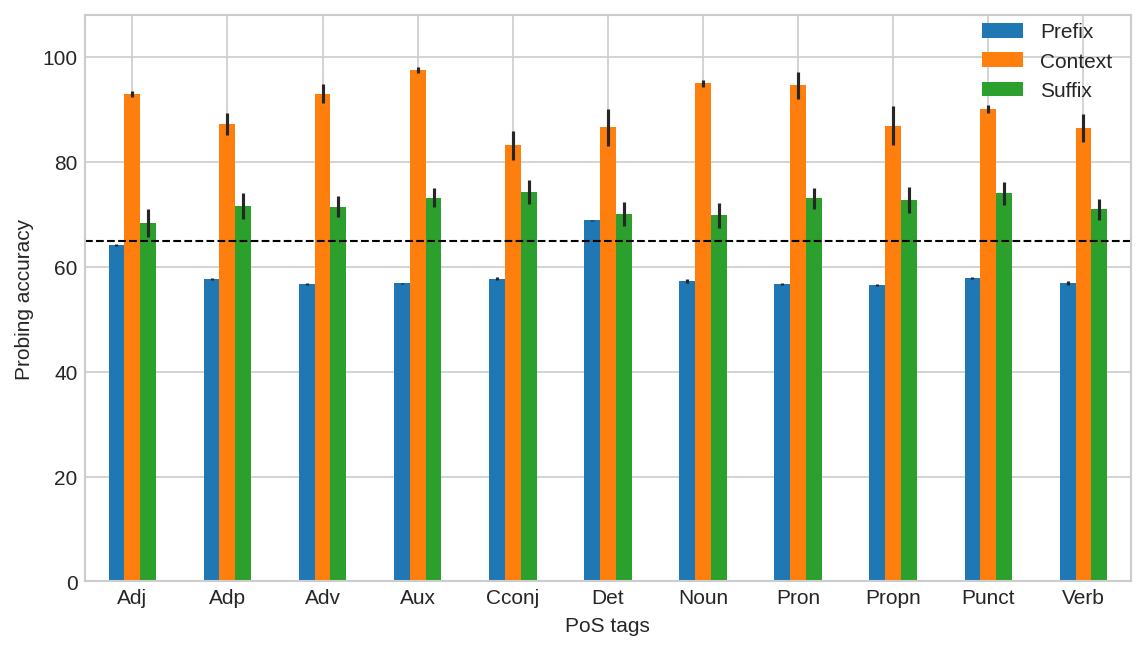
\includegraphics[width=\columnwidth]{figures/probing-all.png}
\caption{Probing accuracy based on tokens PoS tags and their positions in the sentences, from left to right: \emph{prefix}, \emph{context}, \emph{suffix}   }\label{tab:res_per_PoS}
\end{figure}

\begin{table}[ht]
  \centering
  \scalebox{0.85}{
  \begin{tabular}{lcccc}
    \toprule
    
    \multicolumn{5}{l}{\textit{Subject-verb across object relative}}\\
        Subsets &  \makecell{Mask \emph{context} tokens  \\ except \texttt{cue que} }  & Mask \texttt{cue} &Mask \texttt{que}& Mask \texttt{cue$\oplus$que} \\
    \phantom{ab} Overall    & 16.7$_{\pm 0.7}$ & 10.6$_{\pm 1.3}$ & 2.6$_{\pm 0.3}$& 13.5$_{\pm 0.6}$  \\\cline{1-5}
    \phantom{ab} 5 heuristics & 5.0$_{\pm 0.5}$&2.4$_{\pm 0.4}$&0.5$_{\pm 0.1}$&4.0$_{\pm 0.3}$\\
    \phantom{ab} 4 heuristics &15.3$_{\pm 1.0}$&10.1$_{\pm 1.6}$&3.0$_{\pm 0.4}$&12.5$_{\pm 0.6}$ \\
    \phantom{ab} 3 heuristics &28.1$_{\pm 0.8}$&19.8$_{\pm 3.0}$&5.7$_{\pm 0.4}$&24.3$_{\pm 1.1}$\\
    \phantom{ab} 2 heuristics &44.1$_{\pm 1.4}$&21.1$_{\pm 3.2}$&7.0$_{\pm 0.8}$&35.4$_{\pm 1.3}$\\
    \phantom{ab} 1 heuristics &44.7$_{\pm 1.9}$&25.3$_{\pm 2.3}$&3.2$_{\pm 0.6}$&30.8$_{\pm 1.9}$\\
    \phantom{ab} 0 heuristics &42.6$_{\pm 2.0}$&31.1$_{\pm 1.9}$&6.7$_{\pm 1.0}$&34.3$_{\pm 1.9}$\\
     \midrule
    
    \multicolumn{5}{l}{\textit{Object-past participle}} \\

    \midrule
    
    \phantom{ab} Overall      & 8.4$_{\pm 1.0}$ & 25.6$_{\pm 0.8}$  &17.9$_{\pm 0.5}$ &30.1$_{\pm 0.3}$ \\\cline{1-5}
    \phantom{ab} 5 heuristics  & 3.6$_{\pm 0.1}$& 7.8 $_{\pm 0.3}$&6.7$_{\pm 0.2}$ & 10.5$_{\pm 0.5}$\\
    \phantom{ab} 4 heuristics &7.9$_{\pm 1.1}$ & 24.0$_{\pm 0.7}$ & 15.3$_{\pm 0.4}$&27.6$_{\pm 0.4}$\\
    \phantom{ab} 3 heuristics &11.6$_{\pm 1.7}$&24.8$_{\pm 1.4}$&19.4$_{\pm 1.0}$&28.5$_{\pm 0.4}$\\ 
    \phantom{ab} 2 heuristics &12.6$_{\pm 3.3}$&40.5$_{\pm 1.6}$&39.8$_{\pm 1.4}$&53.8$_{\pm 0.5}$\\
    \phantom{ab} 1 heuristic &15.8$_{\pm 3.3}$&67.5$_{\pm 1.4}$&57.7$_{\pm 1.0}$&80.7$_{\pm 0.4}$ \\
    \phantom{ab} 0 heuristic&24.0$_{\pm 3.4}$&59.0$_{\pm 3.1}$&64.0$_{\pm 1.1}$&88.4$_{\pm 1.3}$\\
   
    
    \bottomrule
  \end{tabular}}
  \caption{Average causal effect of interventions on Transformer's NA task performance, quantified by \textbf{drop} in accuracy before and after different interventions, and further broken down based on prediction difficulty measured by the number of heuristics. The term \emph{cue} here refers to the antecedent and its modifiers (determiners and adjectives) in O-PP agreement, and to the subject and its modifiers in S-V agreement.}
    \label{tab:full_causal_res}
\end{table}

\begin{table}[ht]
  \centering
  \begin{tabular}{llcc}
    \toprule
    \multicolumn{2}{l}{Constructions}  &$\mathcal{M}$ & $\mathcal{M}_{NoPos}$ \\
    \midrule
    \multicolumn{2}{l}{Perplexity}   & 27.0   & 27.4   \\
    \midrule
    \multicolumn{4}{l}{\textit{S-V agreement}} \\
    \phantom{ab} & overall  & 98.9\%$_{\pm 0.04}$   & 98.8\% $_{\pm 0.1}$ \\\cline{2-4}
    \phantom{ab} & 5 heuristics  &99.6\% $_{\pm 0.05}$ & 99.6\% $_{\pm 0.1}$ \\
    \phantom{ab} & 4 heuristics  &99.0\% $_{\pm 0.1}$ & 98.5\% $_{\pm 0.2}$ \\
    \phantom{ab} & 3 heuristics  & 98.4\% $_{\pm 0.1}$ & 98.1\% $_{\pm 0.2}$\\
    \phantom{ab} & 2 heuristics  & 97.7\% $_{\pm 0.1}$& 97.6\% $_{\pm 0.1}$\\    
    \phantom{ab} & 1 heuristic &96.8\% $_{\pm 0.1}$& 97.2\% $_{\pm 0.2}$\\
    \phantom{ab} & 0 heuristic &94.1\% $_{\pm 0.5}$ & 94.8\% $_{\pm 0.7}$\\
    \midrule
    \multicolumn{4}{l}{\textit{O-PP agreement}} \\
     & overall  & 94.6\% $_{\pm 0.2}$  & 94.3\% $_{\pm 0.3}$     \\\cline{2-4}
      & 5 heuristics  &99.2\% $_{\pm 0.1}$ & 99.0\% $_{\pm 0.1}$ \\
     & 4 heuristics  &96.5\% $_{\pm 0.1}$ & 95.9\% $_{\pm 0.2}$\\
     & 3 heuristics  & 91.6\% $_{\pm 0.4}$& 91.3\% $_{\pm 0.6}$\\
     & 2 heuristics  & 87.6\% $_{\pm 0.4}$& 87.5\% $_{\pm 0.6}$\\    
     & 1 heuristic &77.9\% $_{\pm 0.8}$& 78.1\%  $_{\pm 1.0}$ \\
     & 0 heuristic  &76.1\% $_{\pm 1.0}$& 75.6\% $_{\pm 1.3}$\\
    \bottomrule
  \end{tabular}
\caption{Autoregressive Transformer LM's accuracy on two NA tasks with and without positional embeddings. \label{tab:TM_nopos}
}
\end{table}

\begin{table}[ht]
  \centering
  \begin{tabular}{llcc}
    \toprule
    \multicolumn{2}{l}{Constructions}  &$\mathcal{M}^{MLM}$ & $\mathcal{M}_{NoPos}^{MLM}$ \\
    \midrule
    \multicolumn{4}{l}{\textit{S-V agreement}} \\
    \phantom{ab} & overall  & 99.3$_{\pm 0.2}$   & 84.9 $_{\pm 0.8}$ \\\cline{2-4}
    \phantom{ab} & 5 heuristics  &99.7 $_{\pm 0.1}$ & 96.7 $_{\pm 0.1}$ \\
    \phantom{ab} & 4 heuristics  &99.3 $_{\pm 0.1}$ & 87.3 $_{\pm 0.3}$ \\
    \phantom{ab} & 3 heuristics  & 99.0 $_{\pm 0.2}$ & 77.1 $_{\pm 0.5}$\\
    \phantom{ab} & 2 heuristics  & 98.6 $_{\pm 0.1}$& 60.1 $_{\pm 1.1}$\\    
    \phantom{ab} & 1 heuristic &98.1 $_{\pm 0.3}$& 46.5 $_{\pm 2.1}$\\
    \phantom{ab} & 0 heuristic &95.5 $_{\pm 0.3}$ & 29.4 $_{\pm 1.8}$\\
    \midrule
    \multicolumn{4}{l}{\textit{O-PP agreement}} \\
     & overall  & 95.1 $_{\pm 0.2}$  & 72.5 $_{\pm 2.3}$     \\\cline{2-4}
      & 5 heuristics  &99.4 $_{\pm 0.05}$ & 92.2 $_{\pm 0.1}$ \\
     & 4 heuristics  &96.7 $_{\pm 0.1}$ & 79.3 $_{\pm 0.7}$\\
     & 3 heuristics  & 92.2 $_{\pm 0.3}$& 55.6 $_{\pm 1.6}$\\
     & 2 heuristics  & 88.4 $_{\pm 0.5}$& 35.4 $_{\pm 1.8}$\\    
     & 1 heuristic &82.2 $_{\pm 0.7}$& 30.3  $_{\pm 4.1}$ \\
     & 0 heuristic  &75.1 $_{\pm 1.1}$& 22.1 $_{\pm 2.5}$\\
    \bottomrule
  \end{tabular}
\caption{Masked Transformer LM's accuracy on two NA tasks with and without positional embeddings. \label{tab:MLM_nopos}
}
\end{table}

\clearpage

\customsection{Grammar and sampling details} \label{app:dataset-generation}

SLOG expands upon the COGS vocabulary, which consists of 503 nouns and 113 verbs, to additionally include \textit{wh}-words (\textit{who, what}) and \textit{that} used as a relative pronoun. In SLOG, for the sake of simplicity, we only consider restrictive relative clauses introduced by \textit{that} regardless of the animacy of the head NPs. For indirect object-extracted instances, we use the preposition stranding structure, such as \textit{the boy that Emma give a cake to}, rather than \textit{the boy to whom Emma gave a cake}.

The dataset includes the 30,000 examples from the initial COGS training set, and new examples that fall into one of the following categories: 
\begin{itemize}[itemsep=0pt, parsep=0pt, topsep=0pt]
    \item Relative clauses within object NPs, equal in number to instances with PP modifications
    \item Subject and object \emph{wh}-questions matching the quantity of their corresponding declarative sentences
    \item An equal number of four-level-nesting recursion constructions as the depth-2 instances in initial COGS
    \item A primitive example for each ditransitive verbs and verbs accepting complement clause (CP) arguments
\end{itemize}

\noindent Finally, the SLOG sampling process excludes sentences with duplicate nouns (e.g. \textit{Emma saw Emma.}).

\customsection{SLOG Full results and additional analyses} \label{sec:analysis_case}

We report the full results of the experiments discussed in Section~\ref{sec:slog_res} in Table~\ref{tab:res_cases}.

\customsubsection{Effect of the reformatted exact-match metric}
\label{app:metric}
All models exhibit higher overall accuracy with the reformatted exact-match evaluation compared to the initial metric, notably pretrained models with an over 10 percentage point increase (Table~\ref{tab:res_cases}). This suggests that the initial exact-match metric may have underestimated model performance.

\begin{table}[ht]
    \centering
    \scalebox{0.75}{
    \begin{tabular}{lccccccc}
    \toprule
    Generalization cases & \multicolumn{2}{c}{ \makecell[c]{Vanilla \\ Transformer}} & \multicolumn{2}{c}{T5}  & \multicolumn{2}{c}{LLaMa}  & AM-Parser \\
    \midrule
    Deeper PP recursion &\exactmatch{13.1$_{\pm 1.5}$} &13.1$_{\pm 1.5}$ &\exactmatch{15.7$_{\pm 0.7}$}&16.6$_{\pm 1.0}$ &\exactmatch{19.8$_{\pm 1.1}$}&20.6$_{\pm 1.0}$ &100.0$_{\pm 0.0}$ \\
    Deeper tail CP recursion &\exactmatch{0.2$_{\pm 0.1}$} &0.9$_{\pm 0.3}$ &\exactmatch{0.8$_{\pm 0.2}$}&5.3$_{\pm 0.4}$ &\exactmatch{3.9$_{\pm 0.4}$} & 12.1$_{\pm 0.7}$&100.0$_{\pm 0.0}$ \\
    Deeper center embedding &\exactmatch{0.0$_{\pm 0.0}$}& 0.0$_{\pm 0.0}$ &\exactmatch{0.0$_{\pm 0.0}$}&0.0$_{\pm 0.0}$ &\exactmatch{0.0$_{\pm 0.0}$}& 0.0$_{\pm 0.0}$&99.5$_{\pm 0.4}$ \\
     Shallower PP recursion& \exactmatch{98.7$_{\pm 0.8}$} & 98.7$_{\pm 0.8}$& \exactmatch{90.2$_{\pm 2.2}$}&93.1$_{\pm 1.9}$ & \exactmatch{97.3$_{\pm 0.9}$}&98.9$_{\pm 0.6}$ &100.0$_{\pm 0.0}$ \\
    Shallower tail CP recursion & \exactmatch{32.6$_{\pm 3.6}$} &55.2$_{\pm 4.2}$ &\exactmatch{44.8$_{\pm 2.8}$}&60.9$_{\pm 2.1}$ &\exactmatch{85.4$_{\pm 3.6}$} & 98.1$_{\pm 0.7}$&100.0$_{\pm 0.0}$ \\
    Shallower center embedding &\exactmatch{0.0$_{\pm 0.0}$} &0.0$_{\pm 0.0}$ &\exactmatch{0.0$_{\pm 0.0}$}&64.1$_{\pm 19.1}$ &\exactmatch{0.0$_{\pm 0.0}$}&50.7$_{\pm 5.7}$ &100.0$_{\pm 0.0}$ \\
    
    \midrule
    PP in subject NPs & \exactmatch{0.0$_{\pm 0.0}$} &0.0$_{\pm 0.0}$ &\exactmatch{0.0$_{\pm 0.0}$}& 0.8$_{\pm 0.5}$&\exactmatch{12.3$_{\pm 4.4}$}& 28.9$_{\pm 3.5}$& 57.6$_{\pm 8.1}$ \\
    PP in indirect object NPs &\exactmatch{42.5$_{\pm 2.2}$}& 42.5$_{\pm 2.2}$ &\exactmatch{50.1$_{\pm 1.7}$}& 53.8$_{\pm 1.4}$&\exactmatch{55.0$_{\pm 3.9}$}& 71.2$_{\pm 4.2}$ &90.4$_{\pm 8.1}$ \\
    RC in subject NPs & \exactmatch{0.0$_{\pm 0.0}$} &0.0$_{\pm 0.0}$ &\exactmatch{0.0$_{\pm 0.0}$}&0.2$_{\pm 0.2}$ &\exactmatch{3.4$_{\pm 1.6}$}& 29.5$_{\pm 3.4}$ &55.8$_{\pm 8.4}$ \\
    RC in indirect object NPs &\exactmatch{34.4$_{\pm 6.0}$}& 34.8$_{\pm 6.1}$ &\exactmatch{35.1$_{\pm 1.9}$}&36.6$_{\pm 2.1}$ &\exactmatch{48.6$_{\pm 1.9}$}& 55.0$_{\pm 2.1}$ &74.4$_{\pm 6.4}$ \\
    \midrule
    Indirect object-extracted RC &\exactmatch{4.7$_{\pm 5.6}$} &4.7$_{\pm 5.7}$ &\exactmatch{0.0$_{\pm 0.0}$}&0.0$_{\pm 0.0}$ &\exactmatch{0.1$_{\pm 0.3}$}& 2.5$_{\pm 3.2}$ &0.0$_{\pm 0.0}$ \\
    Indirect object \textit{wh}-questions  & \exactmatch{35.9$_{\pm 8.3}$}&42.4$_{\pm 13.5}$ &\exactmatch{0.0$_{\pm 0.0}$}&0.4$_{\pm 0.7}$ &\exactmatch{27.9$_{\pm 9.3}$} &73.5$_{\pm 18.4}$ & 41.4$_{\pm 42.4}$ \\
    \midrule
    Active subject \textit{wh}-questions &\exactmatch{96.7$_{\pm 2.6}$}& 97.1$_{\pm 2.4}$ &\exactmatch{90.5$_{\pm 4.0}$}&98.1$_{\pm 1.7}$&\exactmatch{92.8$_{\pm 6.4}$}& 93.3$_{\pm 6.0}$ &99.8$_{\pm 0.6}$ \\
    Passive subject \textit{wh}-questions &\exactmatch{27.4$_{\pm 1.7}$}& 31.9$_{\pm 5.4}$ &\exactmatch{20.3$_{\pm 3.8}$}&100.0$_{\pm 0.0}$ &\exactmatch{4.8$_{\pm 4.5}$}& 15.3$_{\pm 17.5}$ &100.0$_{\pm 0.1}$ \\
    Direct object \textit{wh}-questions &\exactmatch{2.8$_{\pm 3.4}$} &16.0$_{\pm 12}$ &\exactmatch{47.2$_{\pm 1.0}$}&98.5$_{\pm 0.9}$ &\exactmatch{0.5$_{\pm 0.5}$}& 8.6$_{\pm 5.7}$ &29.4$_{\pm 33.5}$ \\
    \textit{Wh}-questions with modified NPs &\exactmatch{17.6$_{\pm 0.9}$}& 17.8$_{\pm 1.3}$ &\exactmatch{20.5$_{\pm 1.0}$}&36.8$_{\pm 0.4}$ &\exactmatch{15.8$_{\pm 0.6}$}& 20.8$_{\pm 2.4}$ &55.6$_{\pm 12.5}$ \\
    \textit{Wh}-questions long movement &\exactmatch{4.0$_{\pm 7.8}$}& 4.9$_{\pm 9.5}$ &\exactmatch{23.3$_{\pm 4.3}$}&24.9$_{\pm 5.1}$ &\exactmatch{0.8$_{\pm 1.4}$}&3.0$_{\pm 4.7}$ & 0.0$_{\pm 0.0}$ \\
    \midrule
    
   
    \textbf{Overall} &\textbf{\exactmatch{24.2$_{\pm 1.0}$}}& \textbf{27.1$_{\pm 2.0}$} &\textbf{\exactmatch{23.4$_{\pm 1.1}$}}&\textbf{40.6$_{\pm 1.0}$} &\textbf{\exactmatch{27.6$_{\pm 1.0}$}}& \textbf{40.1$_{\pm 1.8}$}&  \textbf{70.8$_{\pm 4.3}$} \\
    
    \bottomrule
    \end{tabular}}
    \caption{Mean accuracy (\%) using exact-match is shown in gray, accuracy using reformatted exact-match described in Section~\ref{sec:slog_ex_setup} is shown in black. AM-Parser's graph-based output yields identical scores for both metrics hence only a single column is reported.
    }
    \label{tab:res_cases}
\end{table}

\customsubsection{RC Modifiers in unseen positions} \label{app:RC_modifiers_results}
\begin{table}[t]
    \centering
    \scalebox{0.8}{
    \begin{tabular}{lccccc}
      \toprule
       Generalization cases & \makecell[c]{Long pred-arg \\dependency?} & \makecell[c]{Vanilla \\Transformer} & T5 & LLaMa&\makecell[c]{AM \\parser}   \\
       \midrule
       \makecell[l]{ {\scriptsize Sub-case: Passive indirect objects} \\  \textbf{A fish} \textbf{was given} to  [ a cat that slept ]$_{\textcolor{blue}{\bf iobj}}$. } & \ding{55}  & 72.0$_{\pm 6.6}$  & 74.2$_{\pm 2.7}$   &97.1$_{\pm 1.2}$ & 99.5$_{\pm 0.6}$ \\
       \makecell[l]{ {\scriptsize Sub-case: Indirect object in PP datives  } \\   Emma \textbf{gave a fish} to  [ a cat that slept ]$_{\textcolor{blue}{\bf iobj}}$.} & \ding{55} & 27.0$_{\pm 9.8}$  & 38.9$_{\pm 5.3}$   &72.7$_{\pm 7.8}$ & 99.3$_{\pm 1.1}$  \\
      \makecell[l]{ {\scriptsize Sub-case: Indirect object in double object datives} \\    Emma \textbf{gave} [ a cat that slept ]$_{\textcolor{blue}{\bf iobj}}$ \textbf{a fish}.} & \ding{51} & 7.9$_{\pm 8.5}$ & 0.2$_{\pm 0.2}$   &0.3$_{\pm 0.3}$& 28.9$_{\pm 17.2}$ \\
      \makecell[l]{ {\scriptsize Subject} \\ \  [\textbf{A cat} that slept]$_{\textcolor{blue}{\bf subj}}$ \textbf{ate} a fish. } & \ding{51} & 0.0$_{\pm 0}$ & 0.2$_{\pm 0.2}$ &29.4$_{\pm 3.4}$&51.7$_{\pm 8.4}$\\
      \bottomrule
    \end{tabular}    
    }
    \caption{Performance of RC modification generalization broken down by construction.} 
    \label{tab:cat_1_RC_analysis}
\end{table}

Generalizing RC modifiers to unseen positions presents a similar challenge as PP modification cases, due to unobserved long-distance dependencies. As shown in Table \ref{tab:cat_1_RC_analysis}, all models exhibit a significant performance discrepancy between constructions involving unseen long predicate-argument dependencies and those that do not.

For novel positions that introduce long predicate-argument dependencies, RC modification in the indirect object appears more difficult than in the subject position, contrary to the case with PP modifiers. The primary error pattern (\ref{ex:iobj_RC_error}) demonstrates that models struggle to detect the RC boundary when the relative clause ends with a verb. They systematically misinterpret the indirect object \texttt{a fish} of the main verb \texttt{gave} as the direct object of the adjacent embedded verb \texttt{slept}.  

\customsubsection{Passive subject \emph{wh}-questions} \label{app:subj_q}
For subject \emph{wh}-questions, which exhibit no gap, T5 and AM-Parser perform near-perfectly on both active and passive subject questions. Vanilla Transformer and LLaMa also perform well on active subject questions, but achieve much lower performance on passive subject questions. This performance discrepancy is the most evident in sub-cases where passive subjects function as theme (e.g., (\ref{ex:subj_q_input}))---the vanilla Transformer has near-zero accuracy for these sub-cases, systematically failing to map \emph{wh}-words to `?' as in (\ref{ex:subj_q_error}):  

\begin{exe}
\ex \label{ex:subj_q_input}Input: What was eaten by Emma ?
\begin{xlist}
    \ex \label{ex:subj_q_gold} Gold:  \lform{eat.theme (x$_2$, ?) $\land$ eat.agent (x$_2$, Emma)}
    \ex \label{ex:subj_q_error} Output of Vanilla Transformer and LLaMa:  \lform{eat.theme (x$_2$,  \textcolor{red}{x$_4$}) $\land$ eat.agent (x$_2$, Emma)}
\end{xlist}
\end{exe}

\noindent As discussed in Section~\ref{subsec:am_parser_analysis}, this error pattern may result from the highly imbalanced label distribution in training output space. Both LLaMa and vanilla Transformer are inclined to repeat the substantially more common subsequence \lform{theme($x_i,x_j$)} over \lform{theme($x_i$,?)}. 

 \begin{exe}
\ex \label{ex:iobj_RC_error} Gold LF and model-predicted LF for \textit{Emma gave a cat that slept a fish}:
    \begin{xlist}
        \small{
        \ex \label{ex:iobj_a_dobj_gold_RC} Gold: \lform{give.agent ($x_1$,Emma) $\land$ give.\textbf{recipient} ($x_1,x_3)$ $\land$  give.theme ($x_1,x_7$)$\land$ cat($x_3$) $\land$ cat.nmod (x$_3,x_5$) $\land$ sleep.agent($x_5,x_3$) $\land$ fish($x_7$)}
    \ex \label{ex:iobj_a_dobj_pred_RC} Out: \lform{give.agent ($x_1$,Emma) $\land$ give.\textcolor{red}{theme} ($x_1,x_3)$ $\land$  cat($x_3$) $\land$ cat.nmod (x$_3,x_5$) sleep.agent($x_5,x_3$) $\land$ \textcolor{red}{sleep.theme($x_5,x_7$)} $\land$fish($x_7$) }
    }
    \end{xlist}
\end{exe}

\customsubsection{\emph{Wh}-questions with modified NPs} 
In \emph{wh}-questions with PP and RC modifiers, even though the SLOG training set only contains \emph{wh}-questions with unmodified NPs, all models generalize well (accuracy > 80\%) to direct object NPs with modifiers (e.g., \textit{Who ate a cake on the table?}). These are cases where the modification pattern is observed in training as a part of declarative sentences. In contrast, performance declines when models encounter \emph{wh}-questions with modifiers in the indirect object position (i.e., modification structure not observed as part of declarative sentences). Similarly, for \emph{wh}-questions with subject position modifiers, the performance is very low: both T5 and vanilla Transformers achieve near-zero accuracy, and LLaMa achieves around 5\%.

This observation mirrors the patterns discussed in \S\ref{subsec:long_distance_hard}, attributed to difficulties introduced by unseen subject-verb dependencies across PPs or RCs. In contrast, the structure-aware model exhibits significantly better performance in \textit{wh}-question with subject modification.

\customsection{SLOG: Results of variable-free LFs} \label{app:varfree_res}
\begin{table}[ht]
    \centering
    \begin{tabular}{lcccc}
    \toprule
    Generalization cases & \makecell[c]{Vanilla \\ Transformer} & T5  & LLaMa  \\
    \midrule
    Deeper PP recursion & 7.8$_{\pm 1.8}$ & 63.0$_{\pm 2.9}$ & 90.9$_{\pm 3.3}$ \\
    Deeper tail CP recursion & 1.0$_{\pm 0.5}$ & 46.2$_{\pm 2.6}$ & 44.1$_{\pm 7.9}$ \\
    Deeper center-embedding & 0.0$_{\pm 0.0}$ & 7.8$_{\pm 1.1}$ & 9.4$_{\pm 2}$ \\
    Shallower PP recursion & 98.2$_{\pm 1.6}$ & 99.6$_{\pm 0.9}$ & 100.0$_{\pm 0.0}$ \\
    Shallower tail CP recursion & 89.3$_{\pm 3.3}$ & 99.3$_{\pm 1.6}$ & 100.0$_{\pm 0.0}$ \\
    Shallower center-embedding & 0.1$_{\pm 0.2}$ & 99.8$_{\pm 0.3}$ & 99.8$_{\pm 0.4}$ \\

    \midrule
    PP in subject NPs & 0.2$_{\pm 0.3}$ & 73.2$_{\pm 9.0}$ & 93.4$_{\pm 4.8}$ \\
    PP in indirect object NPs & 29.3$_{\pm 10.7}$ & 97.4$_{\pm 2.1}$ & 98.1$_{\pm 1.9}$ \\
    RC in subject NPs & 0.1$_{\pm 0.1}$ & 60.8$_{\pm 6.3}$ & 73.9$_{\pm 13.5}$ \\
    RC in indirect object NPs & 4.0$_{\pm 1.9}$ & 71.9$_{\pm 0.8}$ & 73.6$_{\pm 3.9}$ \\
    \midrule
    Indirect object-extracted RC & 0.0$_{\pm 0.0}$ & 62.4$_{\pm 7.5}$ & 3.3$_{\pm 2.8}$ \\
    Indirect object \textit{wh}-questions & 34.1$_{\pm 31.1}$ & 93.4$_{\pm 4.8}$ & 83.8$_{\pm 11.3}$ \\
    \midrule
    Active subject \textit{wh}-questions & 99.0$_{\pm 0.5}$ & 99.8$_{\pm 0.3}$ & 96.2$_{\pm 2.6}$ \\
    Passive subject \textit{wh}-questions & 57.3$_{\pm 23.8}$ & 99.9$_{\pm 0.1}$ & 96.0$_{\pm 3.0}$ \\
    Direct object \textit{wh}-questions & 41.8$_{\pm 3.8}$ & 48.4$_{\pm 0.4}$ & 44.1$_{\pm 4.6}$ \\
    \textit{Wh}-questions with modified NPs & 18.1$_{\pm 2.3}$ & 68.0$_{\pm 1.9}$ & 69.4$_{\pm 6.8}$ \\
    \textit{Wh}-questions long movement & 7.4$_{\pm 3.7}$ & 45.6$_{\pm 4.6}$ & 35.7$_{\pm 6.5}$ \\
    \midrule
    Total & 28.7$_{\pm 4.1}$ & 72.7$_{\pm 1.1}$ & 71.3$_{\pm 3}$ \\
    \bottomrule
    \end{tabular}
    \caption{Mean accuracy (\%) on SLOG using the variable-free logical form of \citet{qiu-etal-2022-improving}.}
    \label{tab:res_cases_varfree}
\end{table}

Table~\ref{tab:res_cases_varfree} reports the accuracy on SLOG using variable-free logical forms. The AM-Parser is unable to handle the variable-free format and therefore is omitted. The hyperparameters for the three tested models are the same as the experiments described in Section~\ref{sec:slog_ex_setup}.

The variable-free LF, as discussed in Section~\ref{sec:data_generation} and \citet{wu2023recogs}, exhibits certain limitations and ambiguities which render direct comparisons with variable-based LF results inappropriate. Regardless, all three models achieve higher accuracy scores on the variable-free LFs compared to the COGS LFs, with pretrained models experiencing a particularly significant boost. This aligns with the observations of \citealt{qiu-etal-2022-evaluating}. 

Despite the change in LF, the overall trends and challenges remain consistent. The vanilla Transformer struggles with the same generalization cases, failing to extrapolate to deeper recursion depths and struggling with cases involving unseen long-distance dependencies. Pretrained models, while exhibiting better overall performance, continue to struggle with more structurally complex generalization cases in their respective categories. These include deeper center-embedding, indirect object-extracted RC and \emph{wh}-questions with long movement.



\customsection{Discussion and limitations}

While SLOG offers a targeted and well-controlled approach to assess structural generalization, it presents some limitations.

First, SLOG is a synthetic corpus and covers only a fraction of the diverse structures in English. Furthermore, previous research has demonstrated that the design of \ac{MR} can have a nontrivial effect on model performance in semantic parsing tasks \citep{guo-etal-2019-towards,herzig2021unlocking,qiu-etal-2022-evaluating}. For example, as noted by \citet{wu2023recogs}, the variable indexing scheme may introduce additional semantically irrelevant challenges when assessing structural generalization. SLOG's reformatted exact-match evaluation metric partially addresses this concern by taking into consideration several variations of MRs that are semantically equivalent including MRs that are equivalent up to constant renaming. However, a more comprehensive study of the effect of artifacts from the formalism is left to future work. 

Second, there also exist challenges specific to the evaluation of pretrained models. That is, distributional shift between training and generalization sets intended by SLOG, such as withholding the constructions \textit{PPs modifying subject NPs} from training, is difficult to strictly enforce when pretraining is involved \cite{kim2022uncontrolled}. This potential violation of distributional control makes the interpretation of the obtained results difficult; we cannot disentangle whether generalization success in pretrained models derives from genuine compositional capabilities or simply exposure during pretraining to the target constructions meant to be withheld from the evaluated models. Still, corpus analyses such as \citet{karlsson2007constraints} suggest that deep center-embedding beyond three levels is very rare in naturally occurring data, so it is possible that very deep embedded structures are withheld as intended even from models exposed to large amounts of pretraining data. We hope the additional structural generalization cases that SLOG offers can also help with future work investigating the interaction between structures available in pretraining data and structural generalization.

\end{document}

%unresolved issue: the "Bibliography" and "Appendix" are now included under the last \part in my table of contents: consider using a combination of the \phantomsection and \addcontentsline commands. (# but this still doesn't work)